%10MB

\documentclass[10pt,finnish,a5paper,twoside=semi]{scrartcl}

\usepackage{fontspec}
\usepackage{babel}
\usepackage{microtype}
\usepackage{multicol}
\usepackage{xcolor}
\usepackage{enumitem}
\usepackage{ragged2e}
\usepackage{graphicx}
\usepackage{wallpaper}
\usepackage{lipsum}
\usepackage{tcolorbox}
\usepackage[labelformat=empty]{caption}
\usepackage[export]{adjustbox}
\usepackage{calc}
\usepackage{pstricks}
\usepackage{contour}
\contourlength{2pt}

\definecolor{link}{HTML}{05A8F7}

\usepackage[colorlinks,linkcolor=black,urlcolor=link]{hyperref}

\RedeclareSectionCommands[tocraggedentrytext]{section}

\setlength{\RaggedRightParindent}{\parindent}
\RaggedRight
\setmainfont[Ligatures=TeX]{Arial}
\urlstyle{same}
\definecolor{kuru}{HTML}{f7941e}
\setcounter{secnumdepth}{0}
\setcounter{tocdepth}{2}
\addto\captionsfinnish{\renewcommand{\contentsname}{Tässä numerossa:}}
\addtokomafont{sectionentry}{\normalfont}
\addtokomafont{disposition}{\rmfamily}
\addtokomafont{caption}{\footnotesize}
\setkomafont{subsection}{\normalfont\itshape}
\setenumerate{leftmargin=*}
\setitemize{leftmargin=*}
\frenchspacing
\def\UrlBreaks{\do\/\do-}

\begin{document}
\thispagestyle{empty}

\ThisCenterWallPaper{1.10}{assets/no_auto_compression/kansikuva}

\vspace*{5.70cm}

{\noindent\color{kuru}\begin{tabular}{@{}c@{}}

\includegraphics[width=6cm]{assets/no_auto_compression/logo} \\
\\
\contour{white}{\large\bfseries 1/2024 Kurkisuon Rusakot ry}
\end{tabular}\par}

\clearpage

\ThisULCornerWallPaper{1}{assets/no_auto_compression/sisäkansikuva.jpg}

\noindent \textbf{Tassu 1/2024} \\
\noindent ISSN 0783-1536

\vfill

% \begin{multicols}{2}
\noindent\textbf{Päätoimittaja:}

Tanguy Gérôme

\href{mailto:tanguy.gerome@gmail.com}{tanguy.gerome@gmail.com}

\medskip

\noindent\textbf{Julkaisija:}

Kurkisuon Rusakot ry, Helsinki

\medskip

\noindent Tarkista lippukunnan ajankohtaiset yhteystiedot nettisivuilta:

\href{https://kurkisuonrusakot.wordpress.com/}{kurkisuonrusakot.wordpress.com}

\medskip

\noindent Etu- ja sisäkannen kuvat:

Tanguy Gérôme

\noindent Takakannen kuva:

Tuntematon kolkka

% \columnbreak
\vspace{0.64cm}

\clearpage\tableofcontents
% \end{multicols}

\clearpage\section{Lippukunnanjohtajan tervehdys}

%\medskip

\begin{multicols}{2}

%\columnbreak

\noindent äääää äääää äääää äääää äääää äääää äääää äääää äääää äääää äääää äääää äääää äääää äääää äääää äääää äääää äääää äääää äääää äääää äääää äääää äääää äääää äääää äääääääääääää

öööööööö öööööööö öööööööö öööööööö öööööööö öööööööö öööööööö öööööööö öööööööö öööööööö öööööööö öööööööö öööööööö öööööööö öööööööö öööööööö öööööööö öööööööö öööööööö öööööööö öööööööö öööööööö öööööööö öööööööö öööööööö öööööööö öööööööö! \\

\vspace*{0.50cm}

\null\hfill LPKJ Janne Suomalainen

\end{multicols}


\medskip
\noindent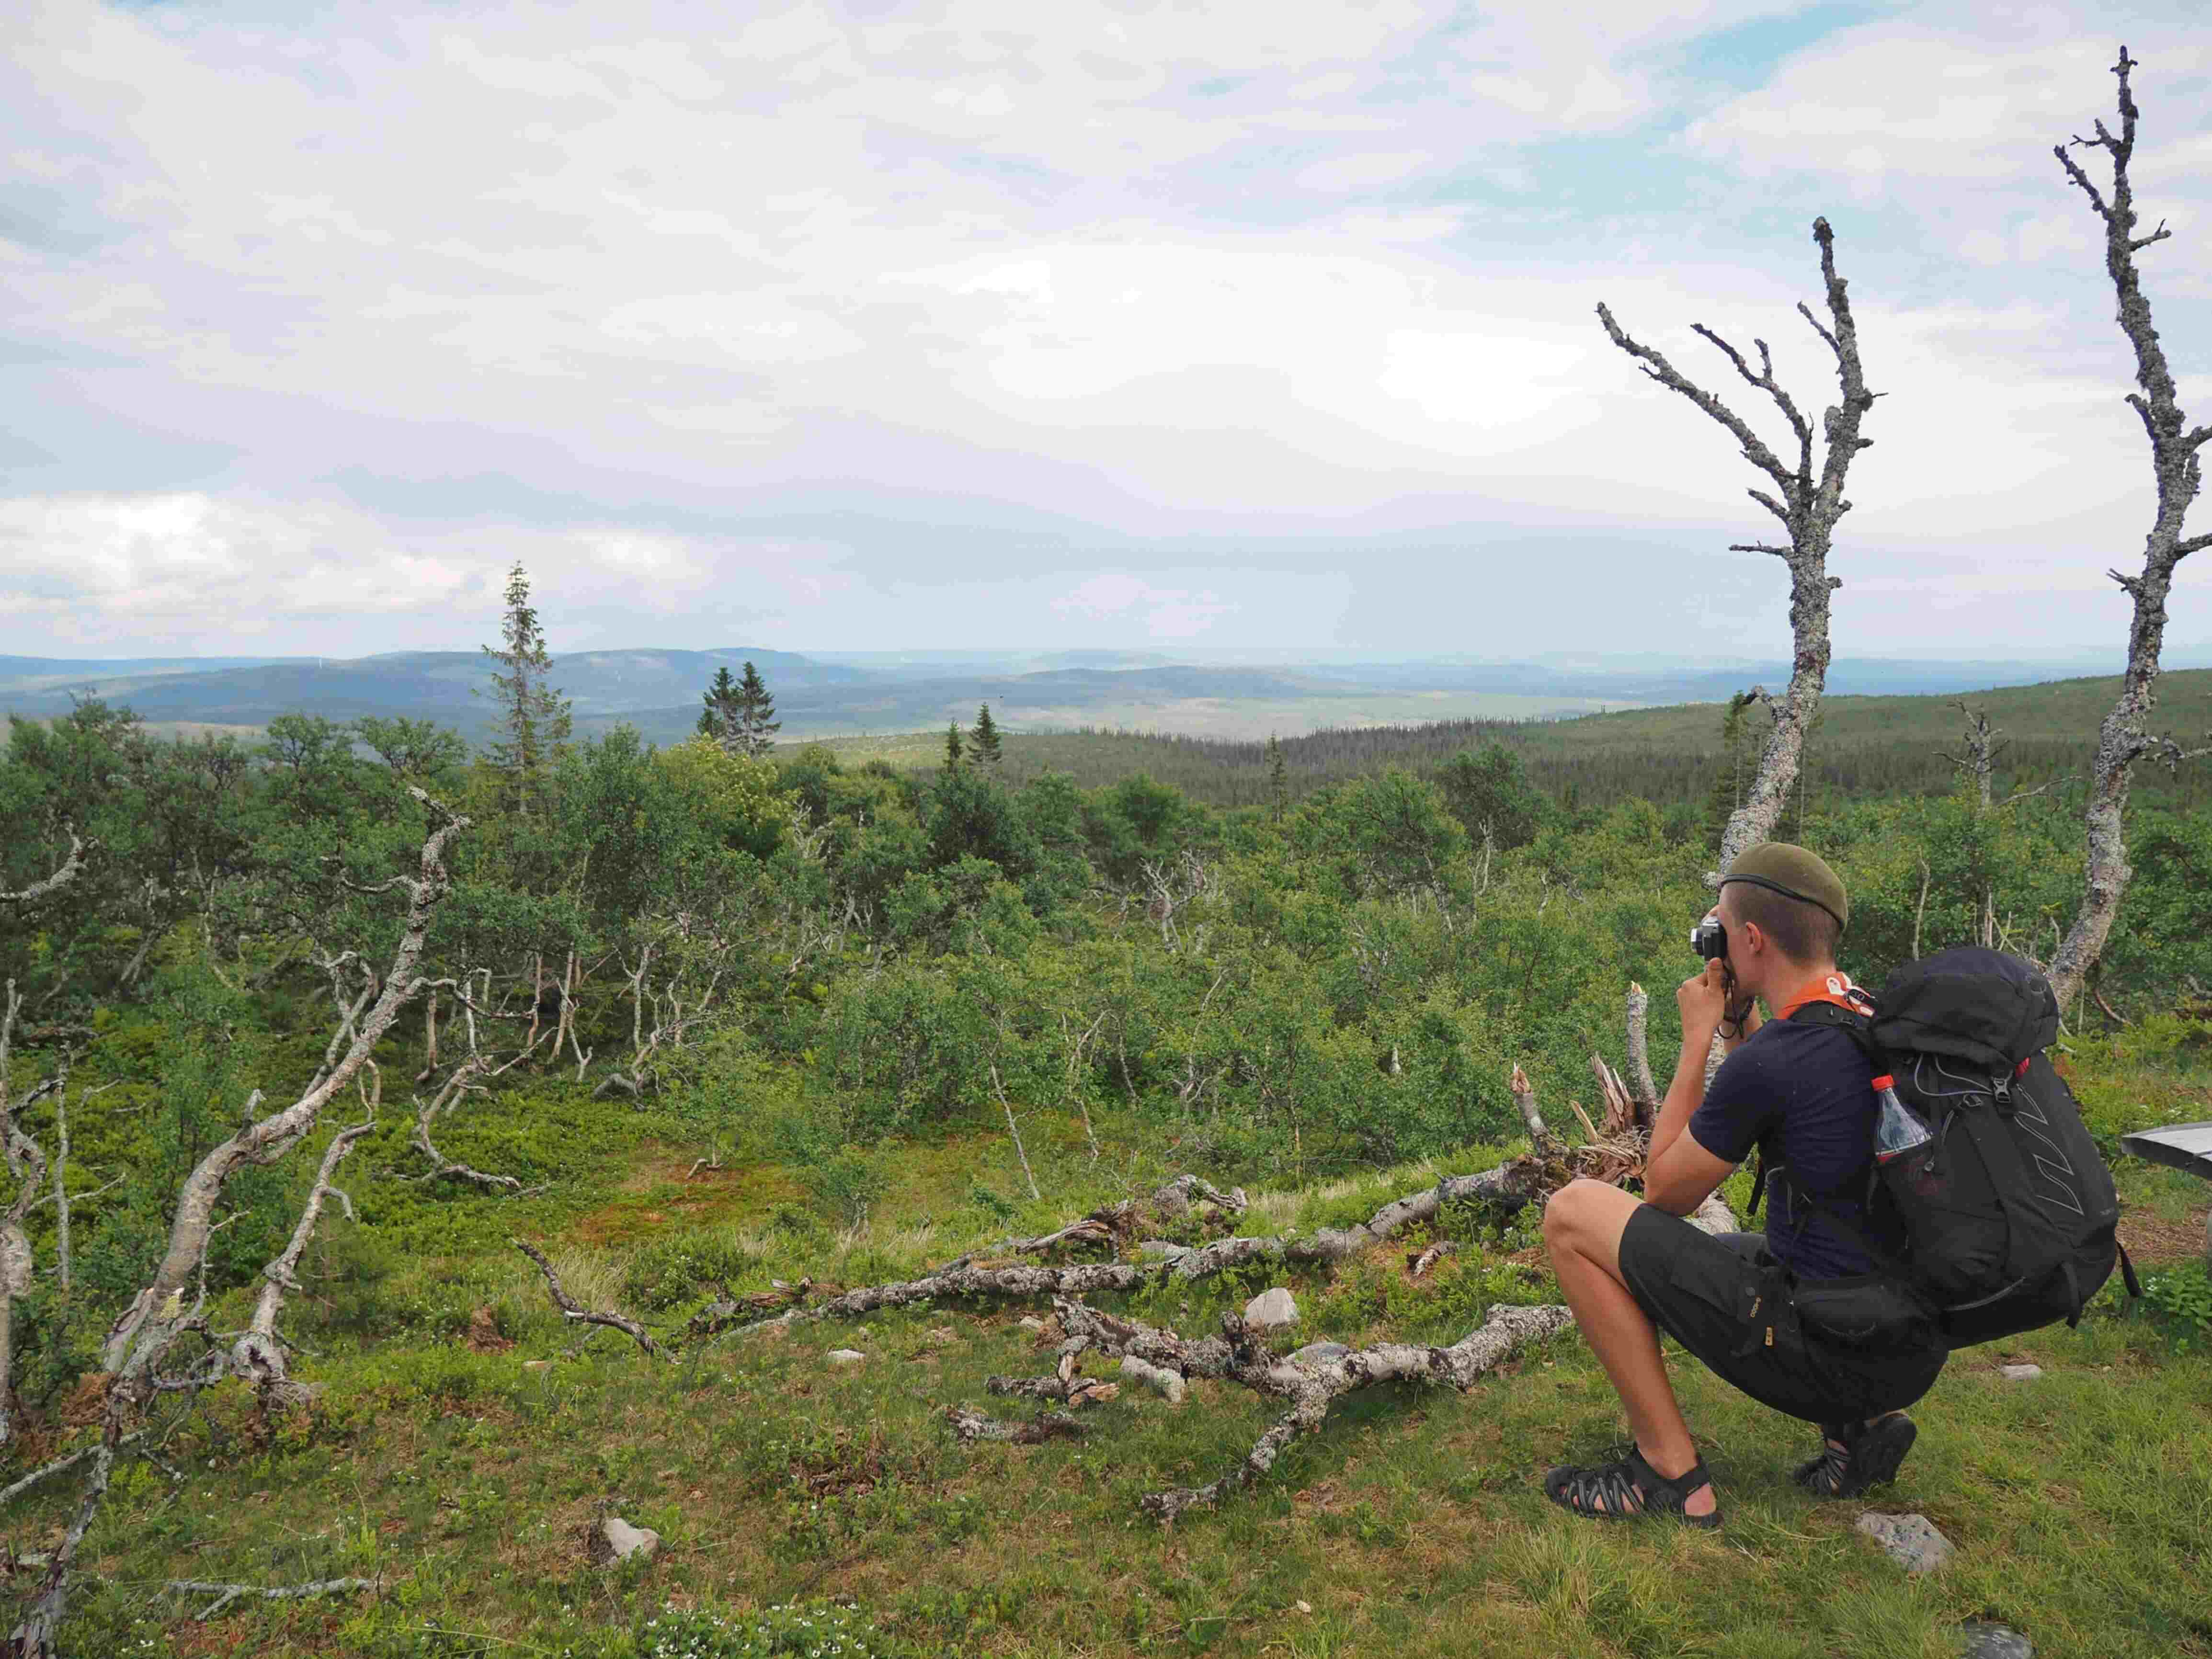
\includegraphics[width=\linewidth]{assets/lpkjtervehdys}

\medskip
\noindent\null\hfill Kuva: Tanguy Gérôme

\clearpage\section{Tassu ennen vanhaan}
\textit{Tassu on ilmestynyt säännöllisen epäsäännöllisesti lippukunnan perustamisvuodesta 1986
lähtien. Tällä palstalla muistellaan menneitä ja julkaistaan valittuja paloja takavuosien
lehdistä.}

\textit{Päätoimittaja sai paketin, jossa on vuosikymmeniä Tassun painoksia ja
yrittää digitalisoida ne lähiaikoina!}


% \clearpage\section{Lippukunnan syksy 2023 nopeasti}
% 	\subsection{ROK}
% 	\subsection{Operaatio olio -telttaretki 6.-8.10.}
% 	\subsection{Hiipivä Haamu 5.11.}
% 	\subsection{Samoajien retki ÄmÄm:n kanssa 10.-12.11.}
% 	\subsection{Pikkujouluretki \& joulujuhla 15.-17.12.}

\clearpage\section{Muistoja vuodelta 2023}
        \subsection{Johtajien kansallispuistokierros Ruotsissa}


\clearpage\section{Lippukunnan kevät 2024}

	\subsection{Lippukunnan yhteinen laskiaistiistai 13.2.}

\begin{multicols}{2}

	\vspace*{0.16cm}
	\noindent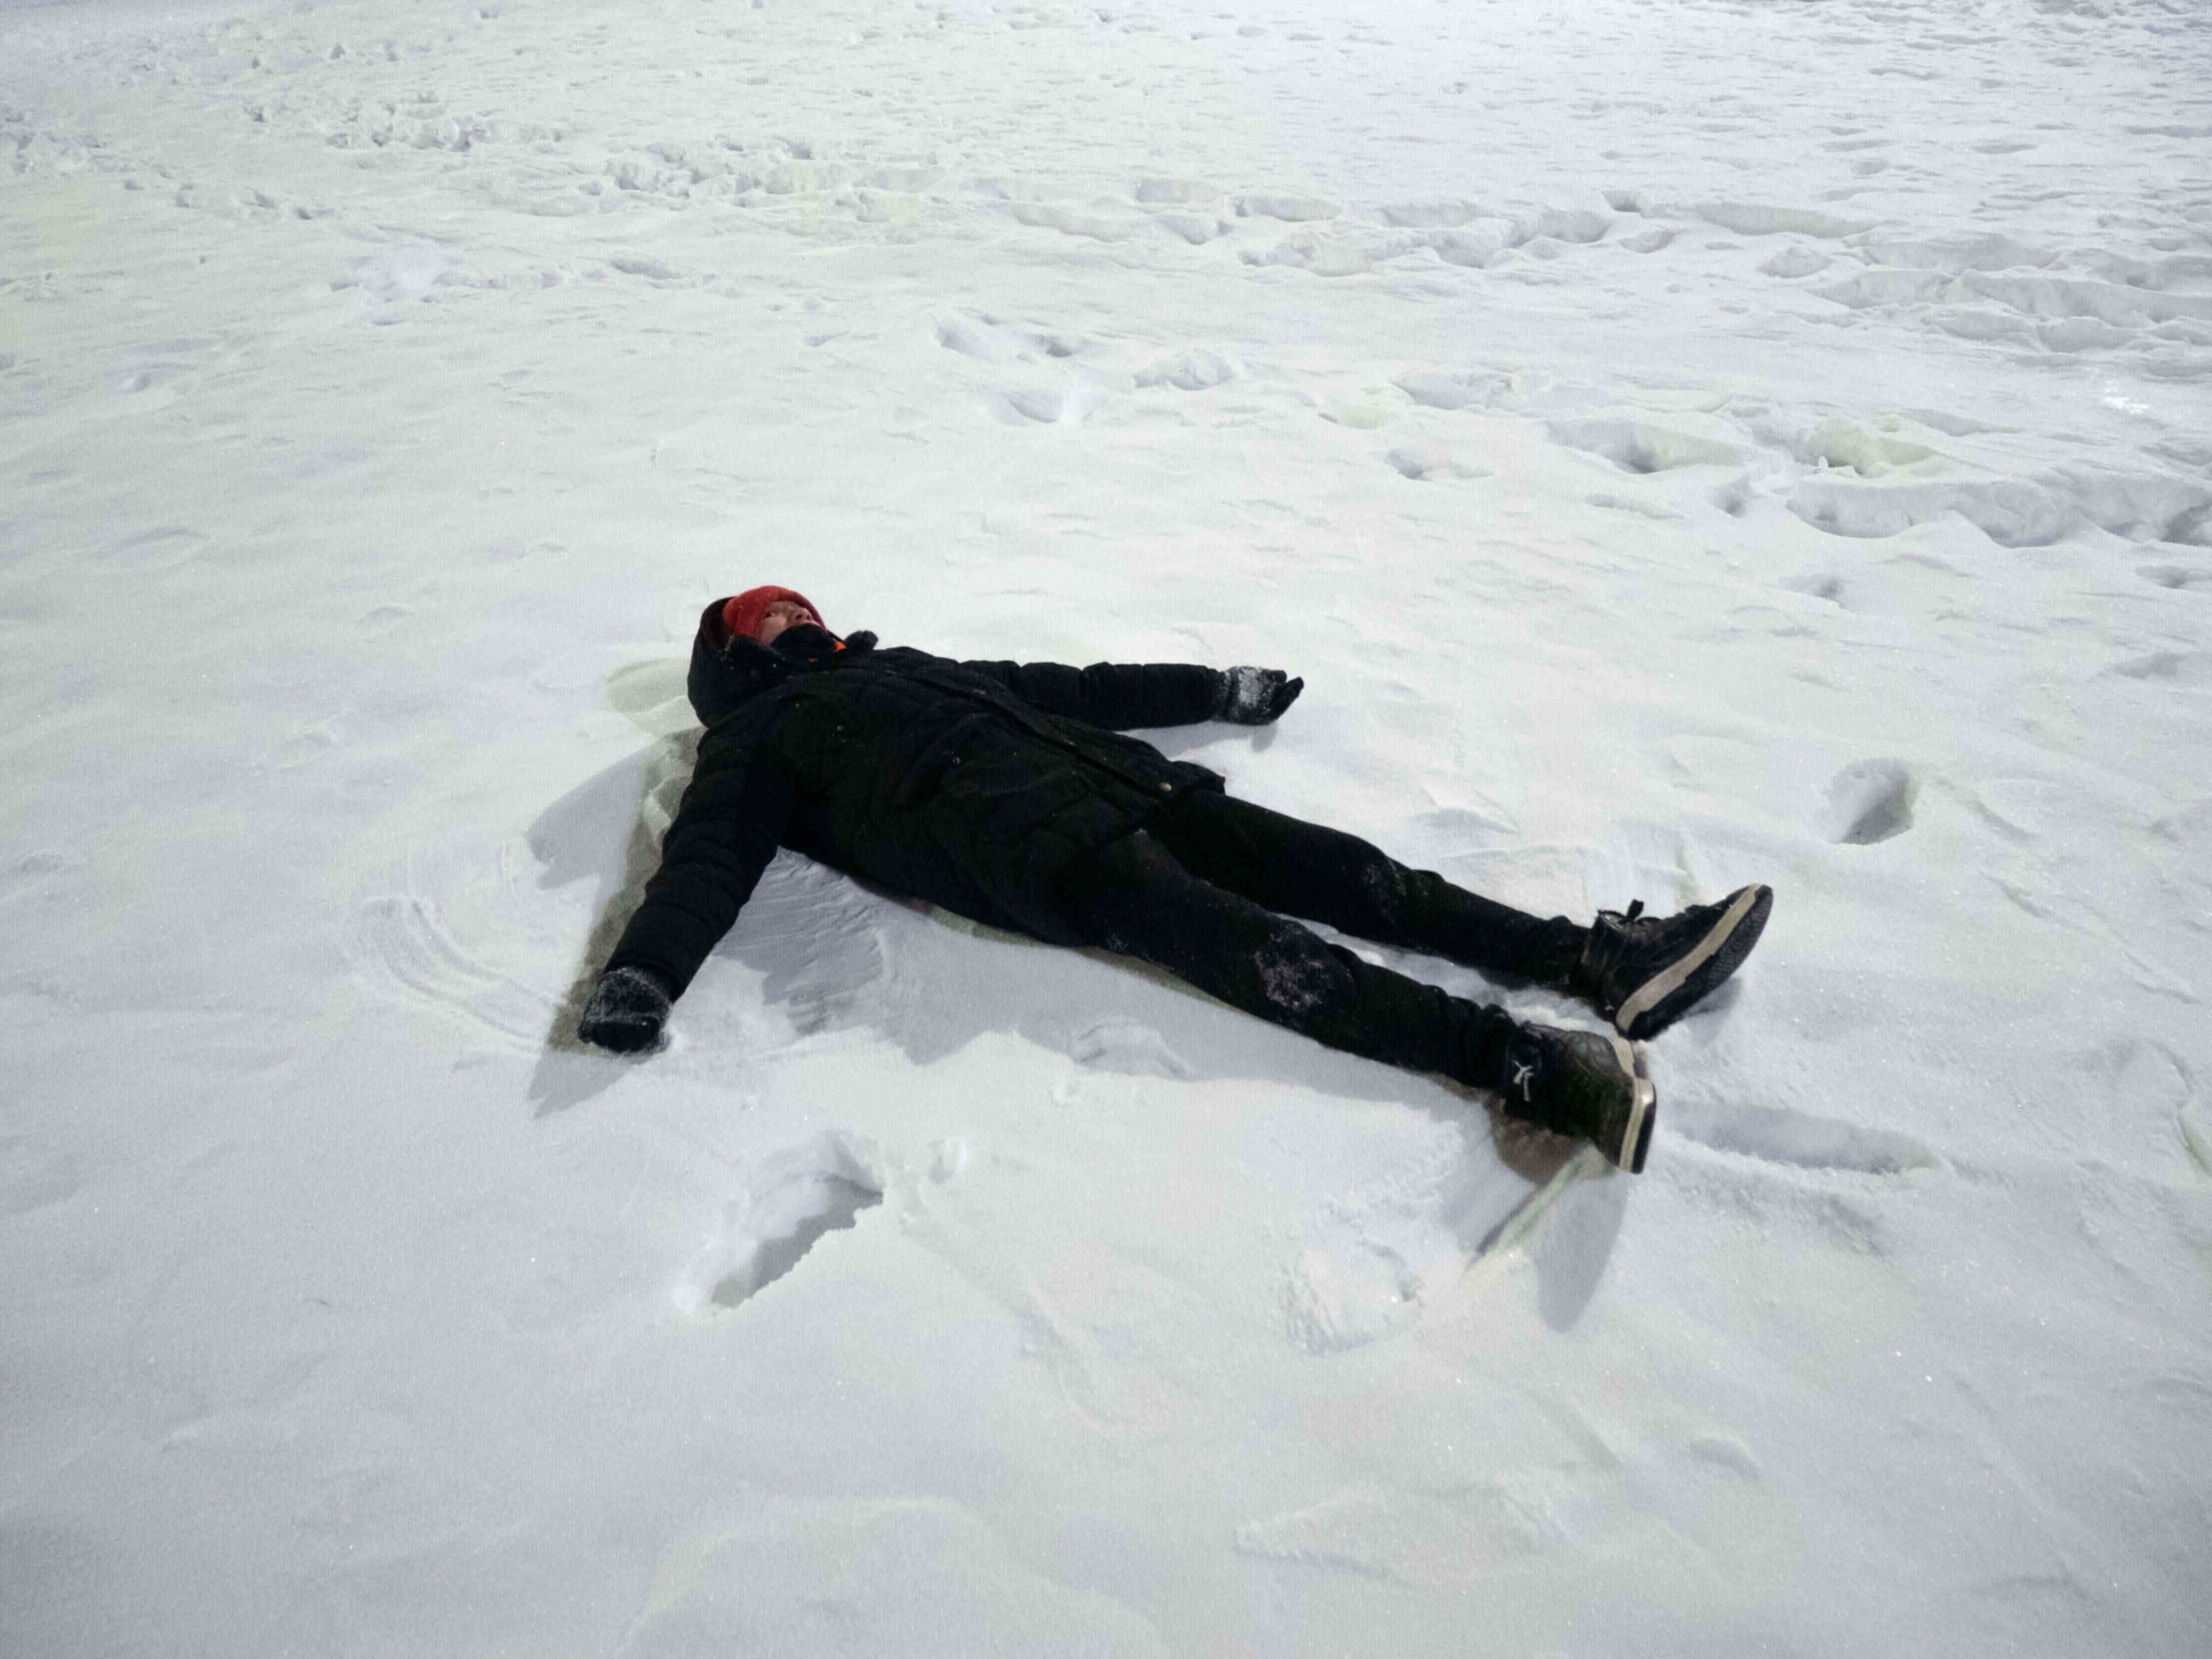
\includegraphics[width=\linewidth]{assets/laskiaistiistai2}

	\small Laskiaistiistai vietimme Kontulan \mbox{kelkkapuistossa}, jossa kaikki
	ryhmät kokoontuivat ja nauttivat kovaa lunta, joka sopi hyviin kelkkailuun, mutta ei niin
	lumienkeleiden tekemiseen \ldots

	\vspace*{1.28cm}
	\noindent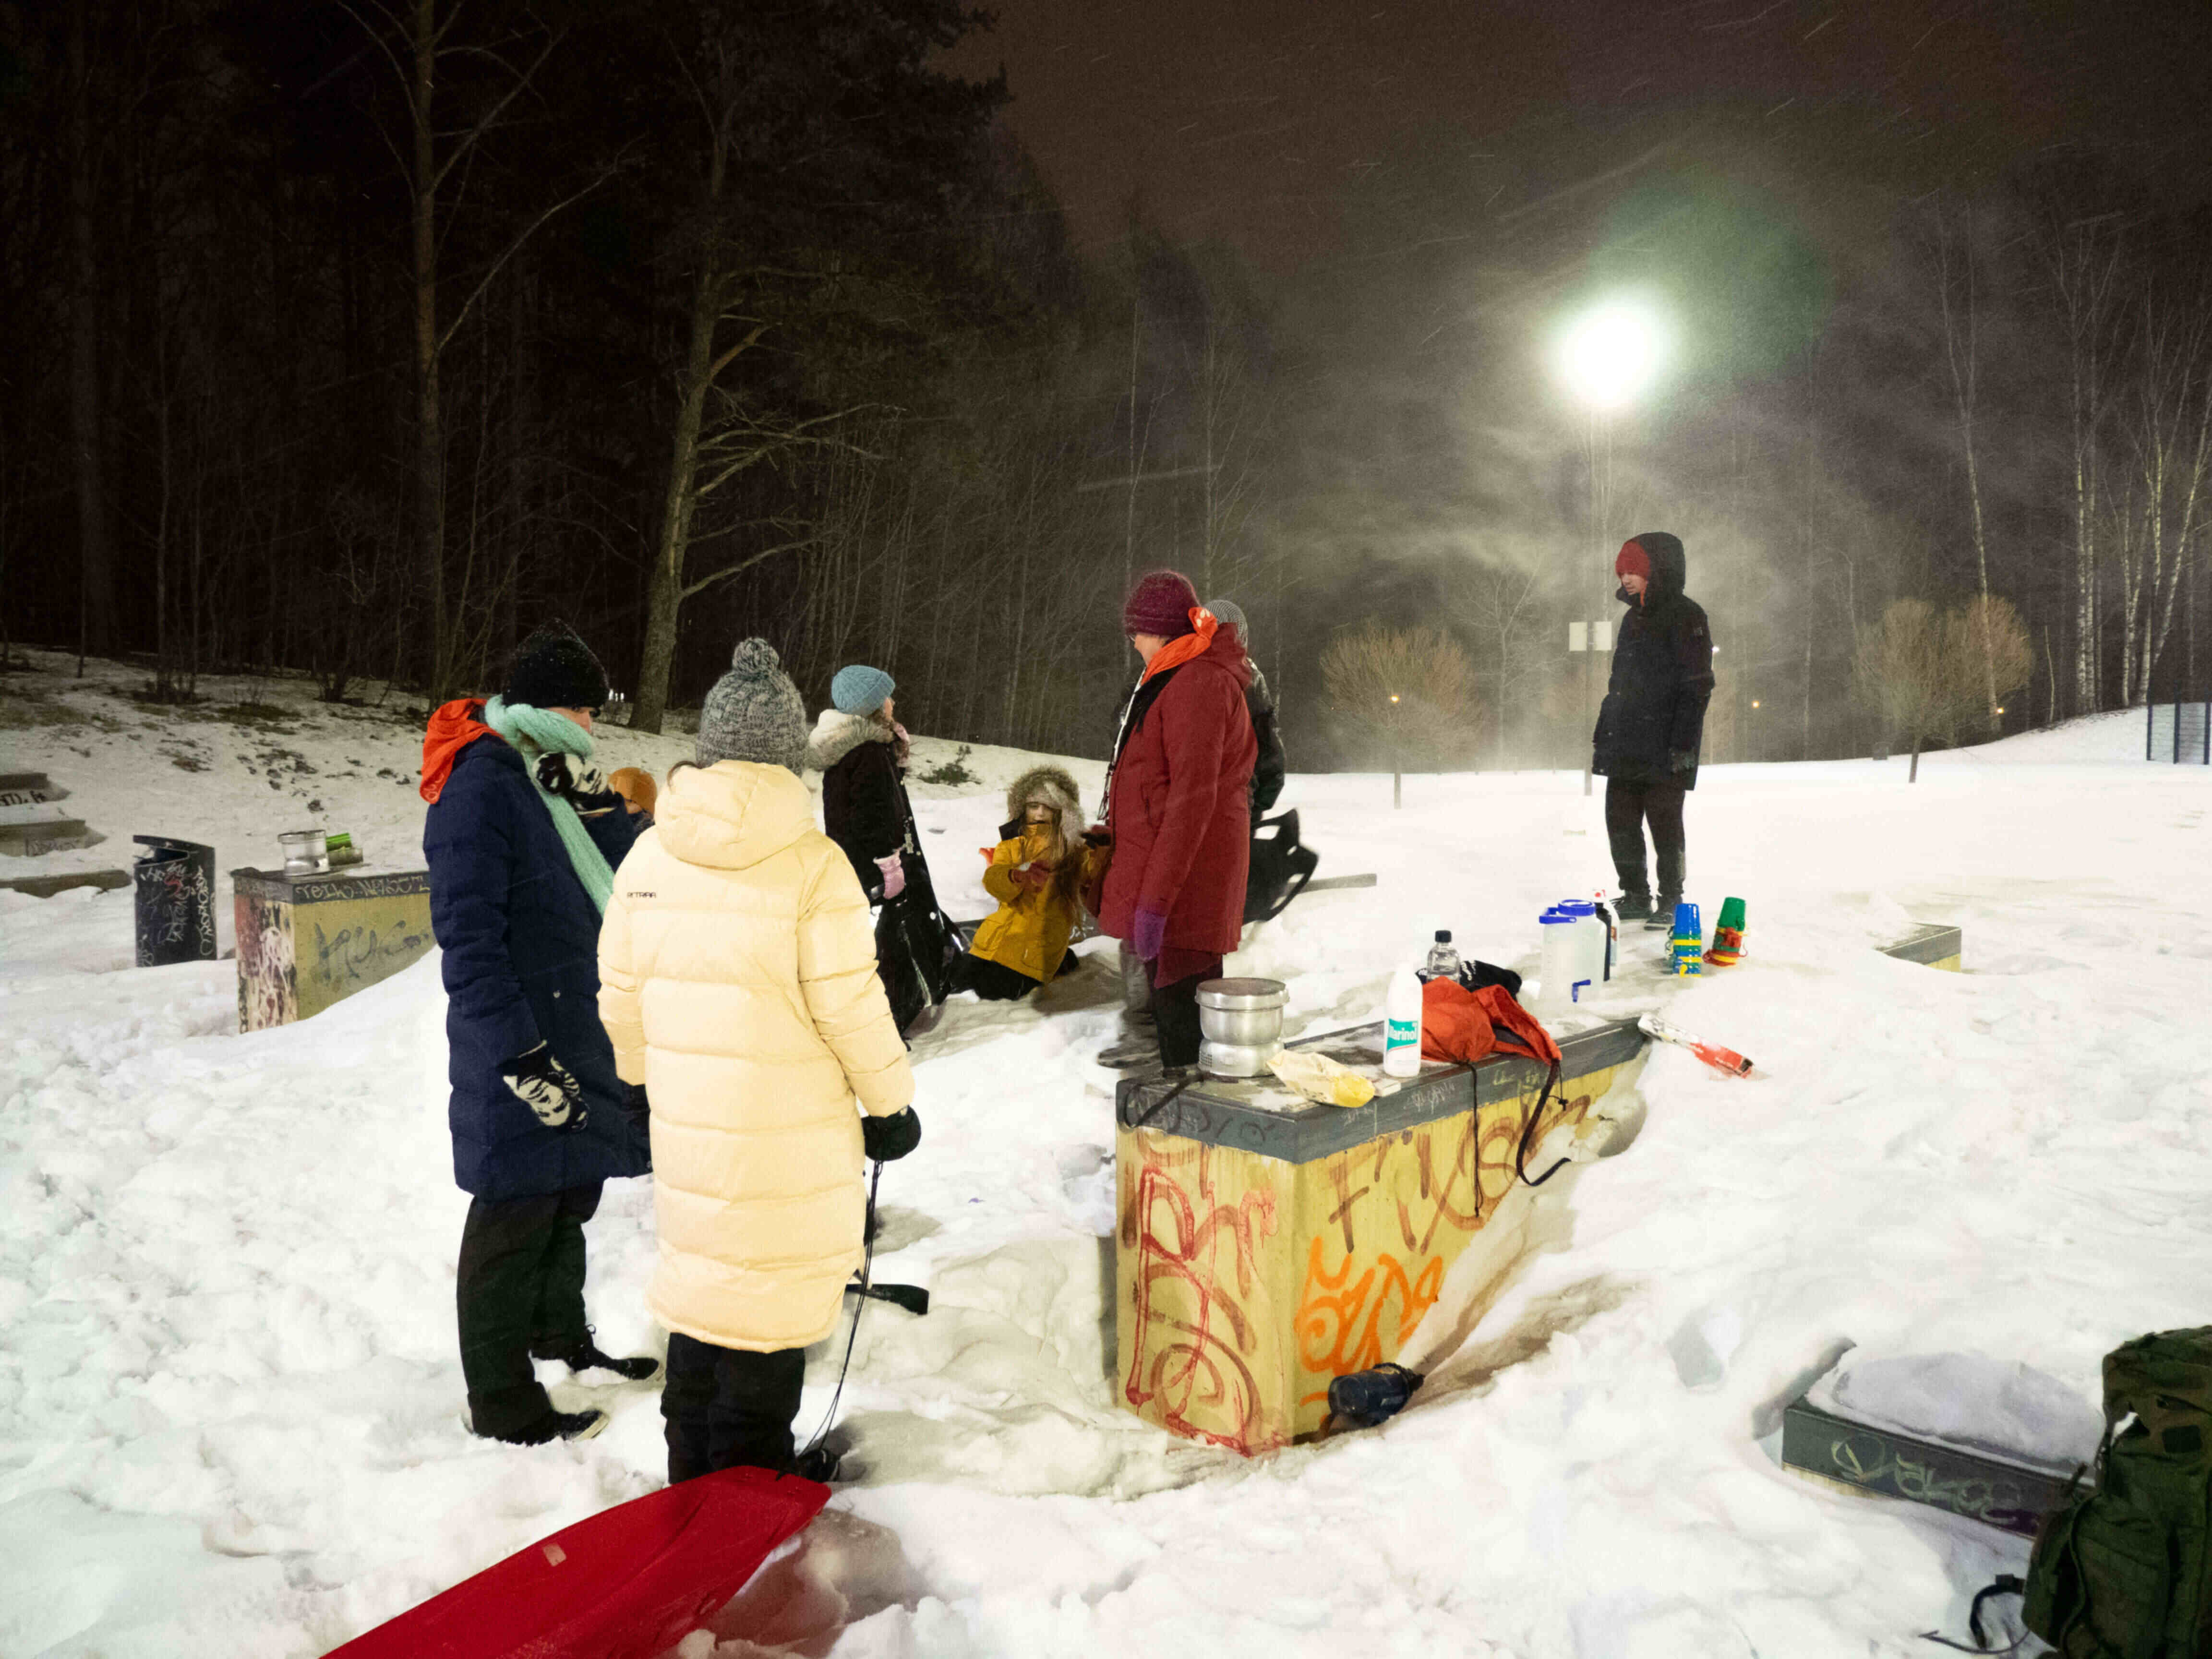
\includegraphics[width=\linewidth]{assets/laskiaistiistai1}

	\ldots ja lämmintä mehua ja keksejä!
	\columnbreak

	\vspace*{1.28cm}
	\noindent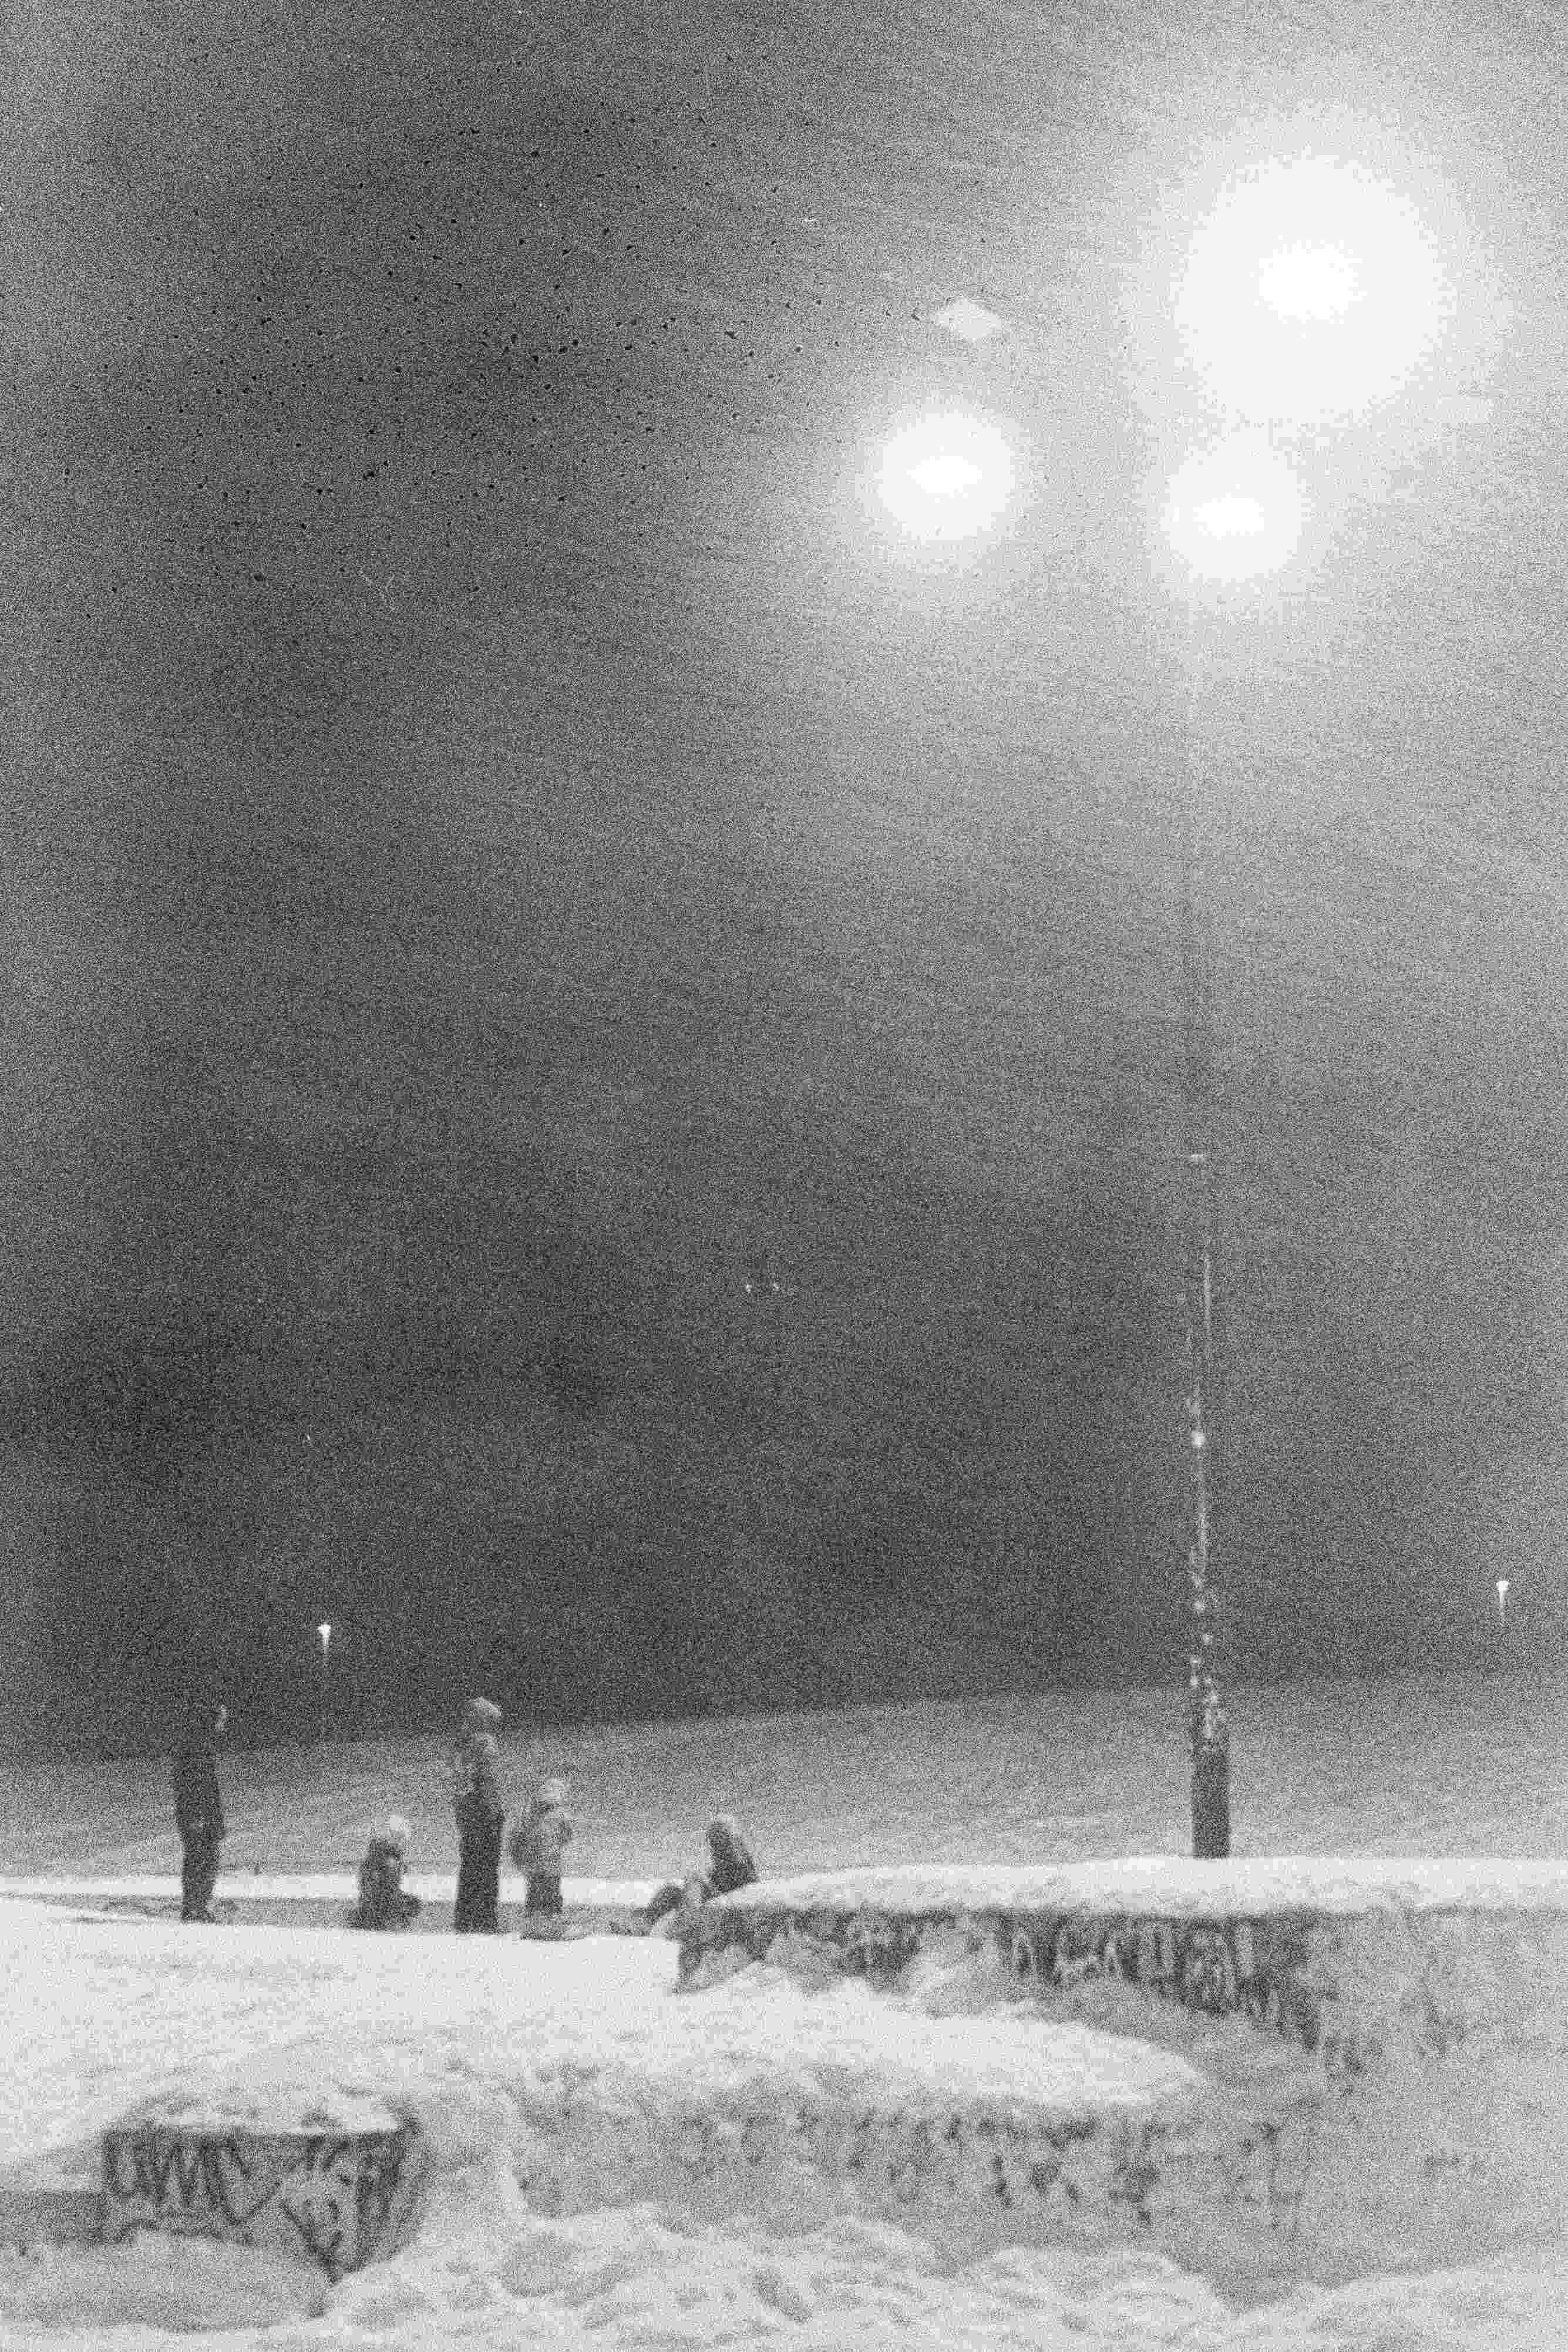
\includegraphics[width=\linewidth]{assets/laskiaistiistai4}

	\ldots todella tuuliset ja talviset kelit \ldots

	\vfill
	\medskip
	\noindent\null\hfill Tanguy Gérôme

\end{multicols}


\section{Vihreä nahkalilja 23.3.}

\begin{multicols}{2}

	\noindent Seitsemän rohkeaa rusakkoa, \mbox{Ahti}, Elias, Janne, Leo, Mikko,
	\mbox{Tanguy} ja Toivo, lähtivät uhmaamaan fyysistä ja henkistä kestävyyttään
	melkein keväisenä maaliskuun aamuna tavoitteenaan taittaa
	neljänkymmenen kilometrin matka vuorokaudessa – niin sanottu vihreä
	nahkalilja. Nahkaliljat ovat vyössä kannettavia partiomerkkejä, joiden
	tarkoituksena on tähdentää ulkoilun merkitystä ja innostaa partiolaisia
	ylläpitämään ja kehittämään peruskuntoaan. Rusakoissa tähdennys ja
	innostus on jäänyt viime vuosina vähemmälle, sillä edellisistä
	nahkaliljoista on ehtinyt vierähtää jo tovi: viimeksi nahkaliljoja on
	vaellettu 26.–27.10.2018, 8.–9.5.2015, 3.–4.5.2014 ja 4.–5.5.2013. Nyt
	kuitenkin innokas porukka on saatu kasaan ja reittimestari Ahti on
	suunnitellut käveltävän reitin Helsingin Mikaelinkirkolta ja takaisin
	paikoin Helsingin itäistä rantareittiä mukaillen – vähän niin kuin
	vuonna 2013, kun allekirjoittanut vaelsi Espoon Rantaraittia
	Kauklahdesta Helsingin keskustaan!

	Vaelluksen lähtö ja maali olivat Mikaelinkirkolla, jonne rusakot
	kokoontuivat aamuyhdeksäksi. Matkaan päästiin vasta \textbf{kello
	9.05}, koska seurue jäi odottamaan kahta nahkaliljaan ilmoittautunutta,
	jotka eivät kuitenkaan ilmestyneet lähtöön. Lähtöaika tarkistettiin
	reittimestarin kellosta ja merkittiin tarkasti muistiin. Niin ikään osa
	osallistujista käynnisti omat satelliitteihin tai muihin antureihin
	tukeutuvat matkamittarinsa, kun taas itse vaellusreitti oli
	perinteikkäästi piirretty karttatulosteelle.

	Liikkeelle lähdettiin kohti Emännänpuistoa ja alustavaksi
	taukostrategiaksi sovittiin, että viiden minuutin taukoja pidettäisiin
	aina viiden kilometrin välein. Harkittiinpa myös ajanvietteeksi laskea
	matkan aikana ylitettävät sillat, joista ensimmäiset tulivat vastaan
	varsin pian, kun ylitettiin Kontulantie ja metron raiteet.

	\vspace*{0.32cm}
	\noindent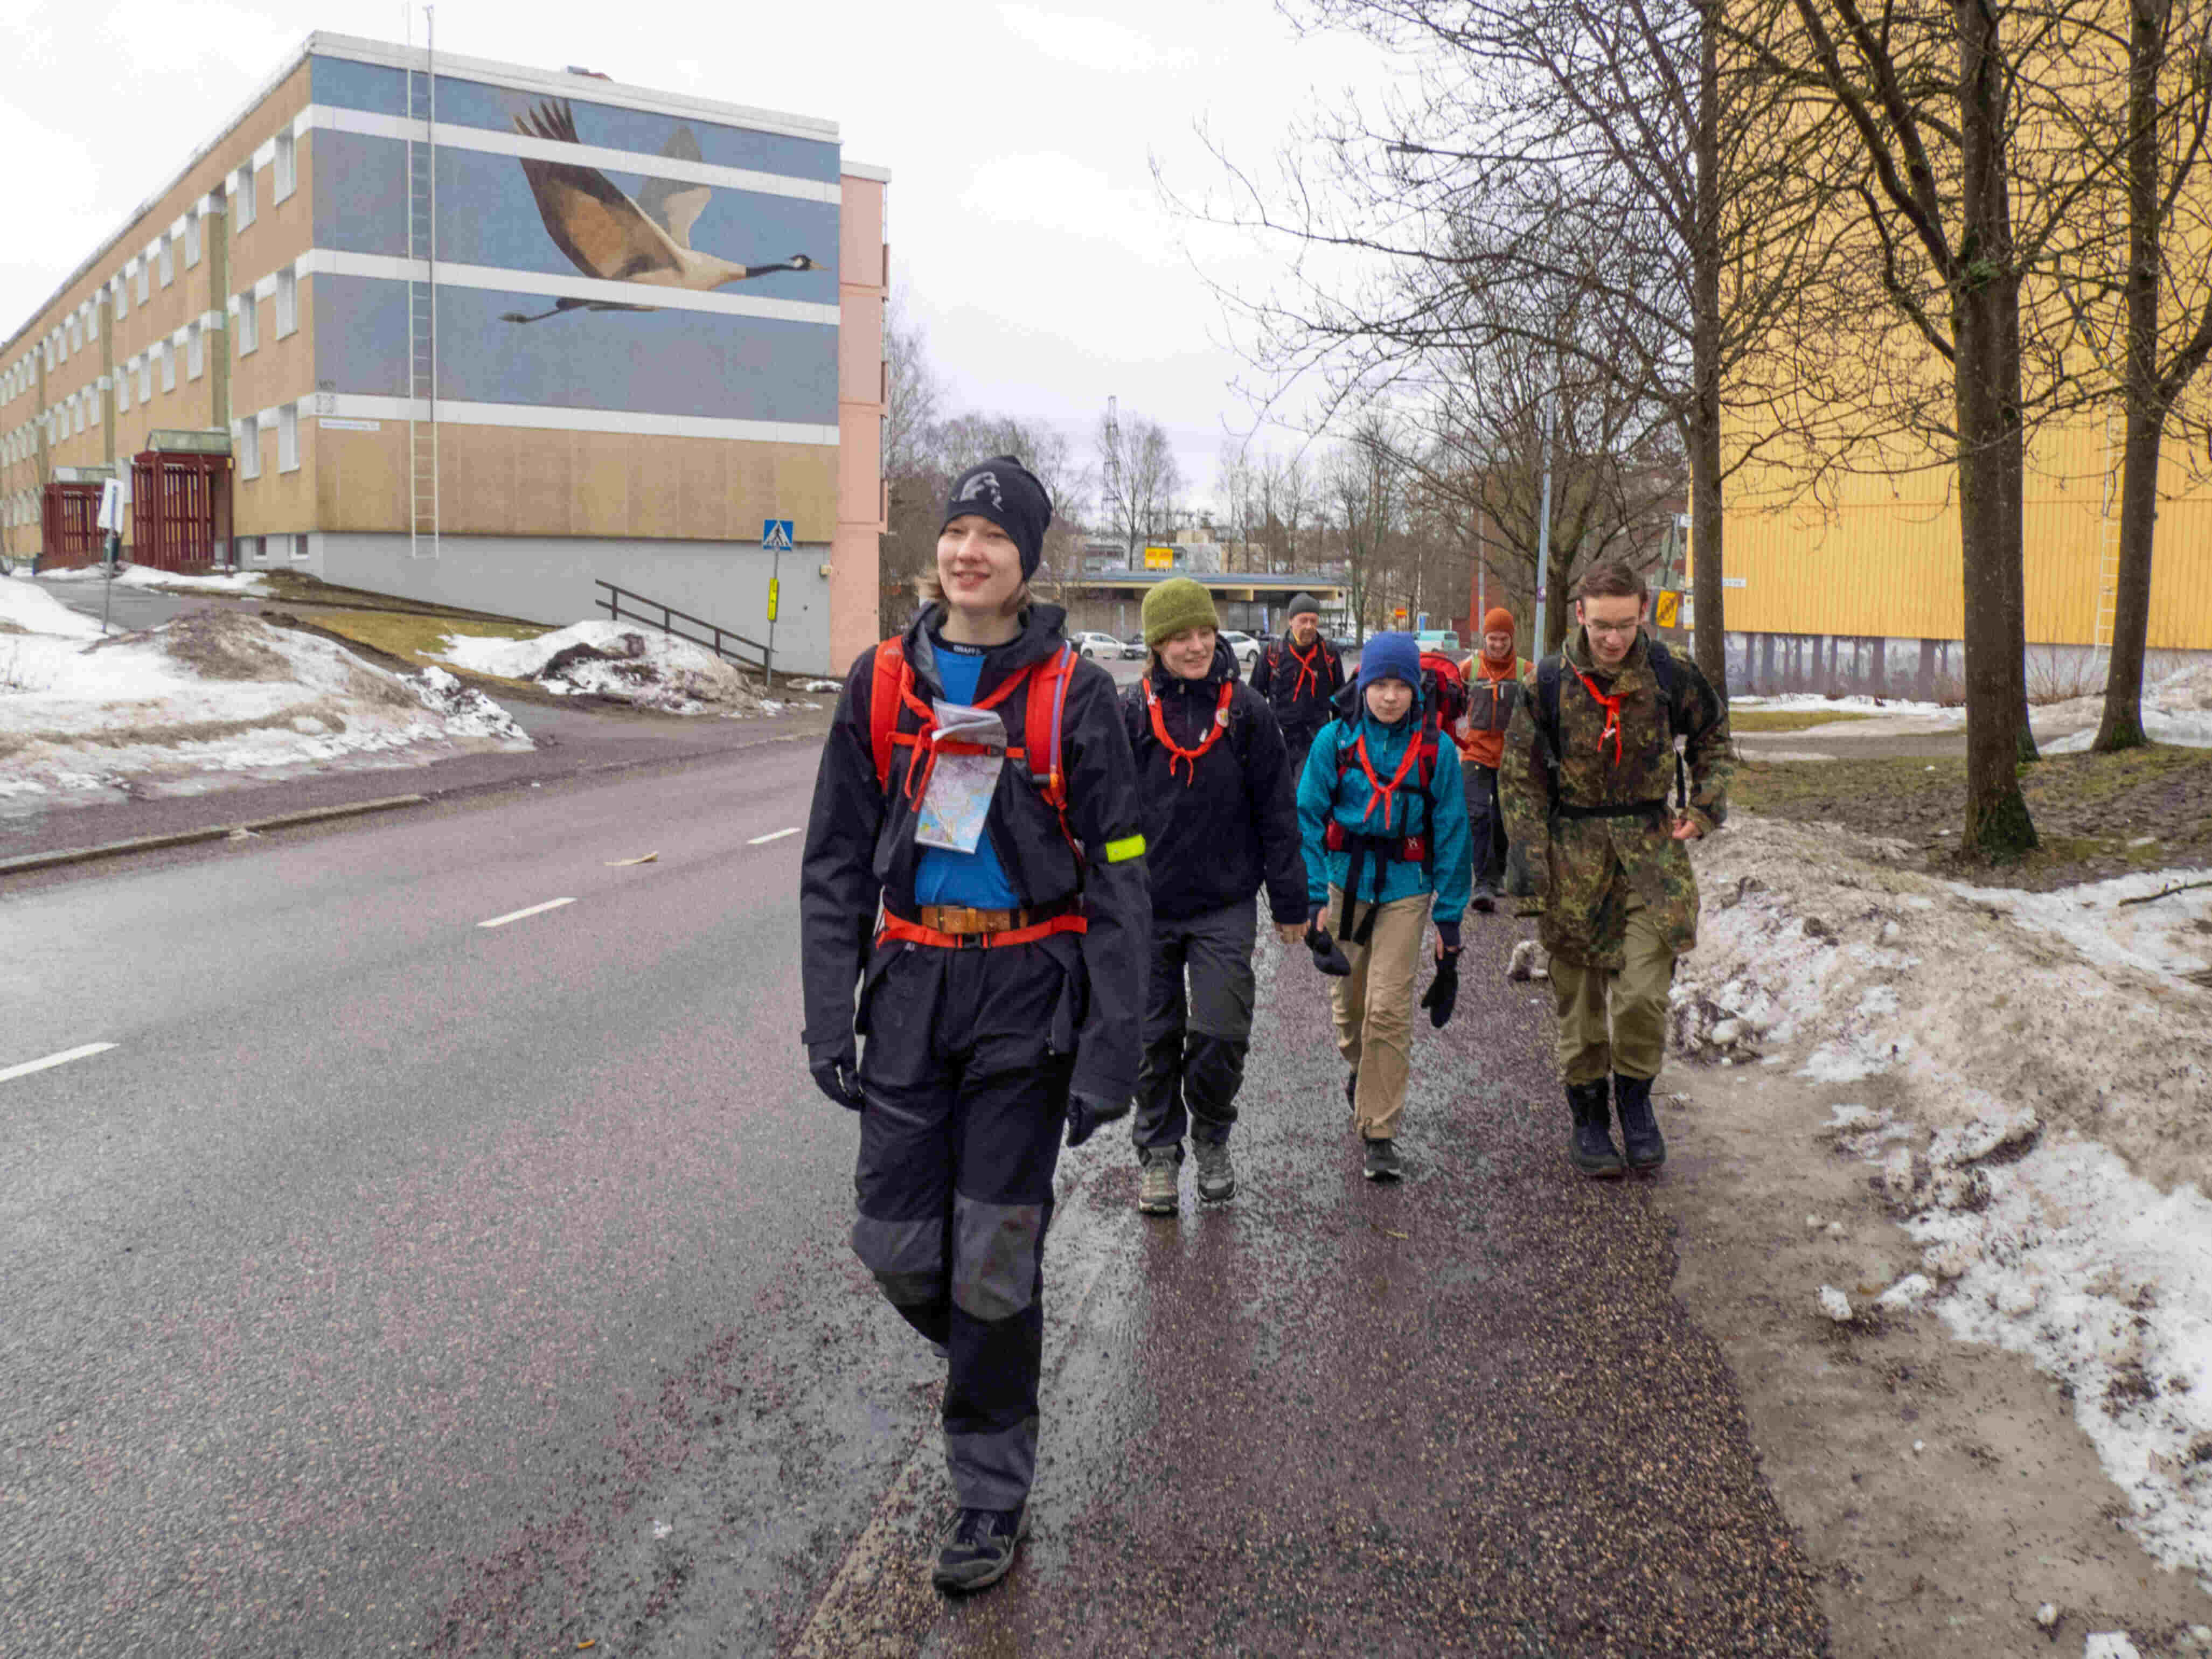
\includegraphics[width=\linewidth]{assets/nahkaliljavantaa}

	Pian oltiinkin jo Vantaan puolella, kun reittimestari ohjasi vaeltajia
	ansiokkaasti Vesalan läpi yli Keihäsrinteen liukkaiden mäkien. Vantaan
	kaupunginosista reitin aikana koettiin kaksi: Rajakylä ja Länsimäki,
	joista – jos ei muuta – saatiin kerättyä muutama silta lisää, ja joista
	ensimmäisessä sijaitsi reitin pohjoisin piste.

	Reitti kaartui jyrkästi etelään ja ensimmäinen poikkeama suunnitellulta
	reitiltä tehtiin tietoisesti \textbf{kello 9.40}, kun vaihdettiin
	puolta Länsimäentiellä pitkin Juoksuhaudanpuiston ylikulkukäytävää
	viheralueelle, jonka läpi menevä ulkoilutie oli varsin kostea.
	Kuntopolku aiheutti hilpeyttä osassa osallistujista, koska tie ei ollut
	kovinkaan pitkä. Vaelluksen ensimmäinen suunnittelematon poikkeama
	tehtiin \textbf{kello 9.52}, kun Keilapolun alikulkukäytävä ylitettiin
	kahteen kertaan.

	Pian oltiinkin takaisin Helsingin puolella. Likimain Mellunmäentien ja
	Naulakalliontien risteyksessä Tanguy huudahti ensimmäisen viiden
	kilometrin merkin, minkä jälkeen alettiin etsiä soveltuvaa
	taukopaikkaa. Sellainen löydettiin Naulakallionpuistosta, jossa
	pysähdyttiin evästämään ja ottamaan ryhmäkuva. Tauko päättyi
	\textbf{kello 10.14}.

	\vspace*{0.32cm}
	\noindent\includegraphics[width=\linewidth]{assets/nahkaliljaryhmä}

	Reitti jatkui kaakkoon, seisahdus Itäväylällä ja jo
	Linnavuorenpuistossa \textbf{kello 10.38} alettiin arpoa, kuinka monen
	sillan yli sitä oli mentykään. Kävelyalusta oli talven aikana
	ladutettu, eli tiiviiksi tampattua nyt jo märkää ja jäätynyttä lunta.
	Onneksi tie Vartiokylänlahden toisella puolella oli paljon
	käveltävämmässä kunnossa. Taktisesti seuraava tauko pidettiin jo
	Vuosaaren sillan kupeessa odottaen seuraavaa etappia läpi Puotilan,
	Marjaniemen ja Roihuvuoren. Eväät maistuivat hyvin eikä kenenkään askel
	painanut tavanomaista enempää. Tauolla pohdittiin läheisen rakennuksen
	seinässä ollutta vSv"-lyhennettä. (Toim. huom. oikea vastaus olisi
	ollut Vuosillan Veneilijät.)

	Vuosaaren sillalla ihmeteltiin uhkarohkeaa pilkkiosastoa, joka
	keväisestä maaliskuun lauantaista huolimatta eteni Vartiokylänlahdella
	\textbf{kello 11.16}. Mikko kuvasi toimintaa nasevasti yhdellä sanalla:
	"Luonnonvalinta." Jo useamman kerran reitti ohitti kaupungin hienot
	opaskyltit itäisestä rantareitistä, joka – nyt jälkikäteen ajatellen –
	voisi olla ihan hauska retki sekin.

	Marjaniemessä ihmetystä aiheutti Vanhalla Koivuniementiellä olleen
	asuinrakennuksen voimakkaasti heijastavat seinäpaneelit, joista
	varmasti naapurit olivat mielissään. Leikkipuisto Iso-Antin nimen
	alkuperää yritettiin tavata Tapio Rautavaaran sanoin "Isontalon Antti
	ja Rannanjärvi / Ne jutteli kaharen kesken". Todennäköisempää lienee
	kuitenkin, että leikkipuisto on saanut nimensä viereisestä Ison-Antin
	tiestä, josta \mbox{Helsingin kadunnimet (1992)} osaa kertoa seuraavaa:

	"Ison-Antin tie — Stor-Andersvägen, 1949. Nimi käytössä jo ennen 1946
	asussa Antintie — Andersvägen, Marjaniemen huvilayhdyskunnan
	perustaja-asukkaihin kuuluneen rakennusmestari Antti Hongiston mukaan,
	jota kutsuttu »Isoksi Antiksi»."

	Nimistökysymyksen jälkeen reitti jatkui länteen. Roihuvuoren rajalla
	alkoivat kuulua ensimmäiset merkit kävelyn aiheuttamasta rasituksesta,
	kun joidenkin vaeltajien jalat alkoivat painaa. Jyrkkä käännös etelään
	ja Tammisalon kanavan yli, Pyörökiventien varressa muuan mies lapioiden
	levitti lunta pihallaan ja pyysi seuruetta talkoisiin. Mikko kieltäytyi
	kohteliaasti kertoen miehelle matkaa olevan jäljellä vielä
	kolmekymmentäviisi kilometriä.

	Likimain viidentoista kilometrin tauko osui Kiiltomadonpuistoon – josta
	kertovasta kyltistä Toivon oli saatava kuva – \textbf{kello 12.22},
	jolloin osa seurueesta vaihtoi jalkaansa kuivat sukat ja kevensi
	varustustaan pilvien välistä pilkottelevan auringon lämmittävän
	vaikutuksen takia.

	Tauon jälkeen jatkettiin vielä etelään, kunnes saavutettiin reitin
	eteläisin piste, Kettu Repolaisen puisto, jossa reitti teki
	u-käännöksen palaten mantereen puolelle Laajasalon siltaa pitkin.
	Seuraava tauko tulikin tavanomaista nopeammin reilu kolme kilometriä
	myöhemmin, kun seurue pysähtyi istumaan Laivalahdenkaaren ja
	Kerttulinkujan kulmassa kasvavan hevoskastanjan alle noin \textbf{kello
	13.15}. Tauko kulki nimellä "Piolimatkankrouvi", vaikka todellisuudessa
	ei sitä ihan vielä ollutkaan. Tulipa seuruetta ihmettelmään muuan
	rouva, joka uteliaisuuttaan tuli kysymään, mistä lippukunnasta
	vaeltajat olivat.

	% \vspace*{0.16cm}
	\noindent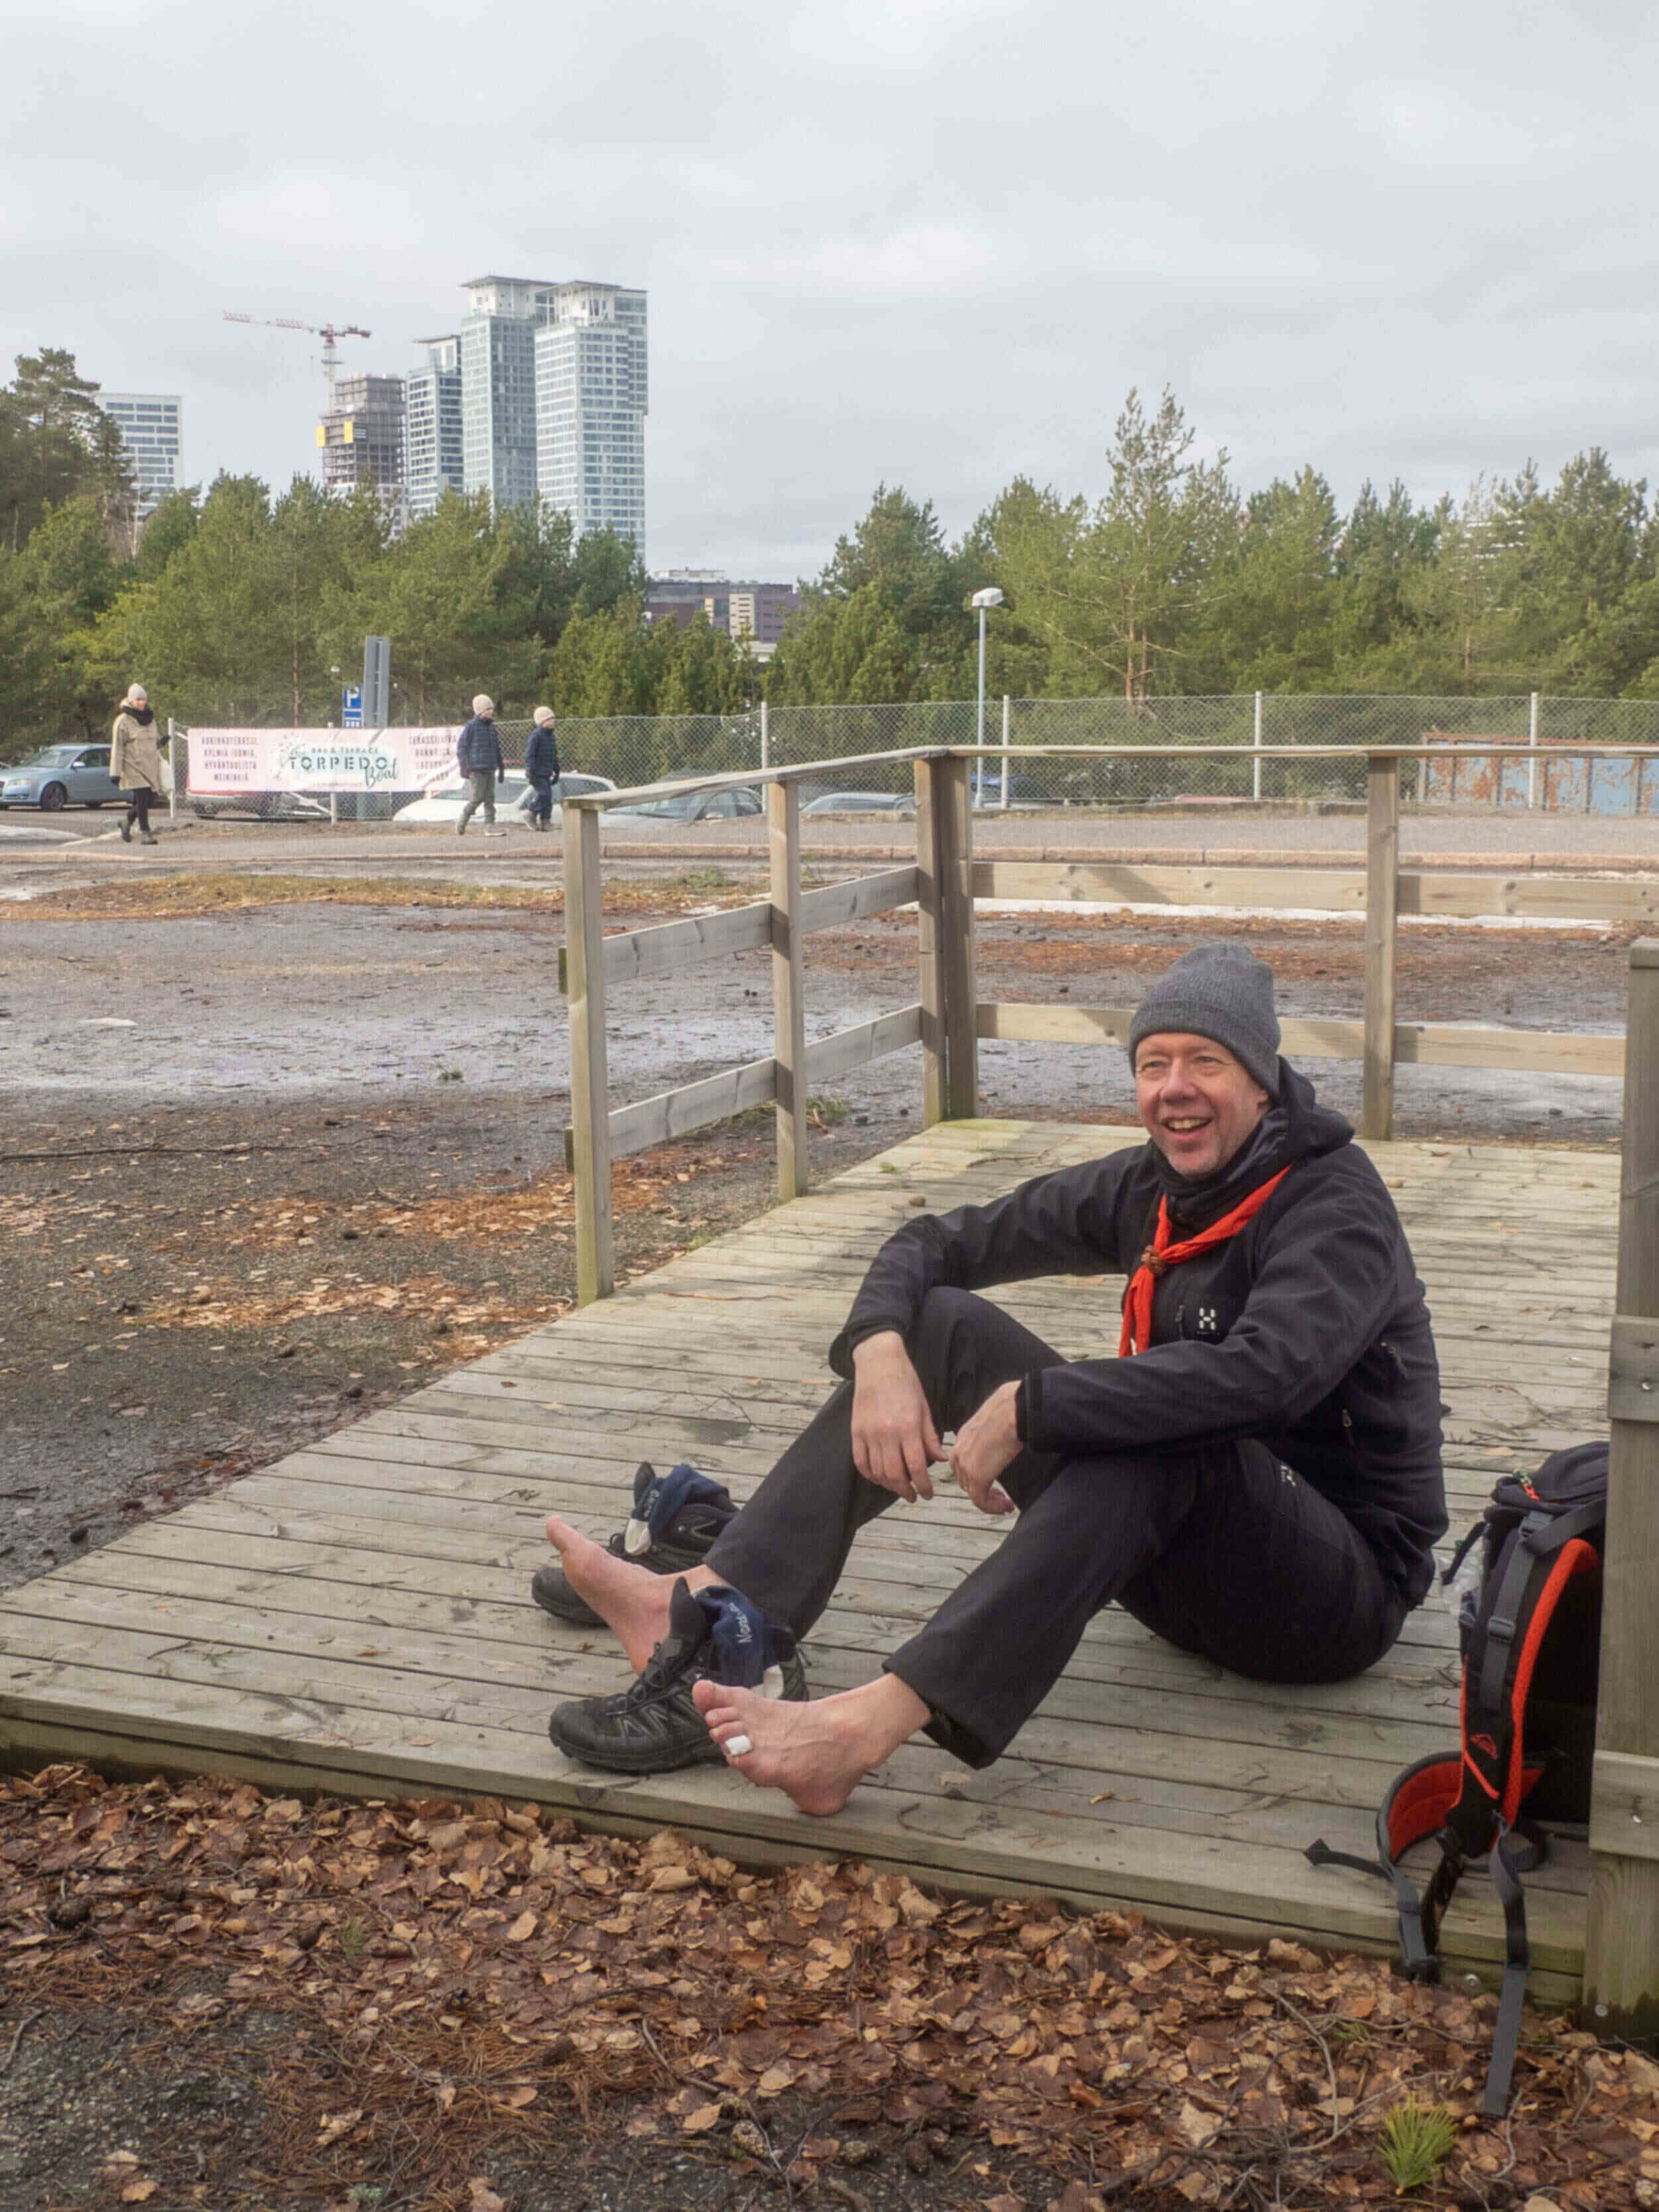
\includegraphics[width=\linewidth]{assets/nahkaliljamikko}

	Nopea taktinen tauko Hitsaajankadun Picnic-kahvilassa ja pian oltiin
	matkalla kohti kaupungin keskustaa. Varustusta lisättiin ennen
	Naurissaaren siltaa kolean länsituulen viilentäen vaeltajia. Läpi
	Kulosaaren, seuraava tauko ja seuraava rouva osuivat Mustikkamaalle
	\textbf{kello 14.28}. Kruunusiltojen työmaata ihmeteltiin ylitettäessä
	Isoisänsiltaa, josta reitti yhtyikin vuoden 2022 Hiipivä Haamu
	-salapoliisikilpailun ennakkotehtävien kaupunkikierrokseen.

	% \vspace*{0.16cm}
	\noindent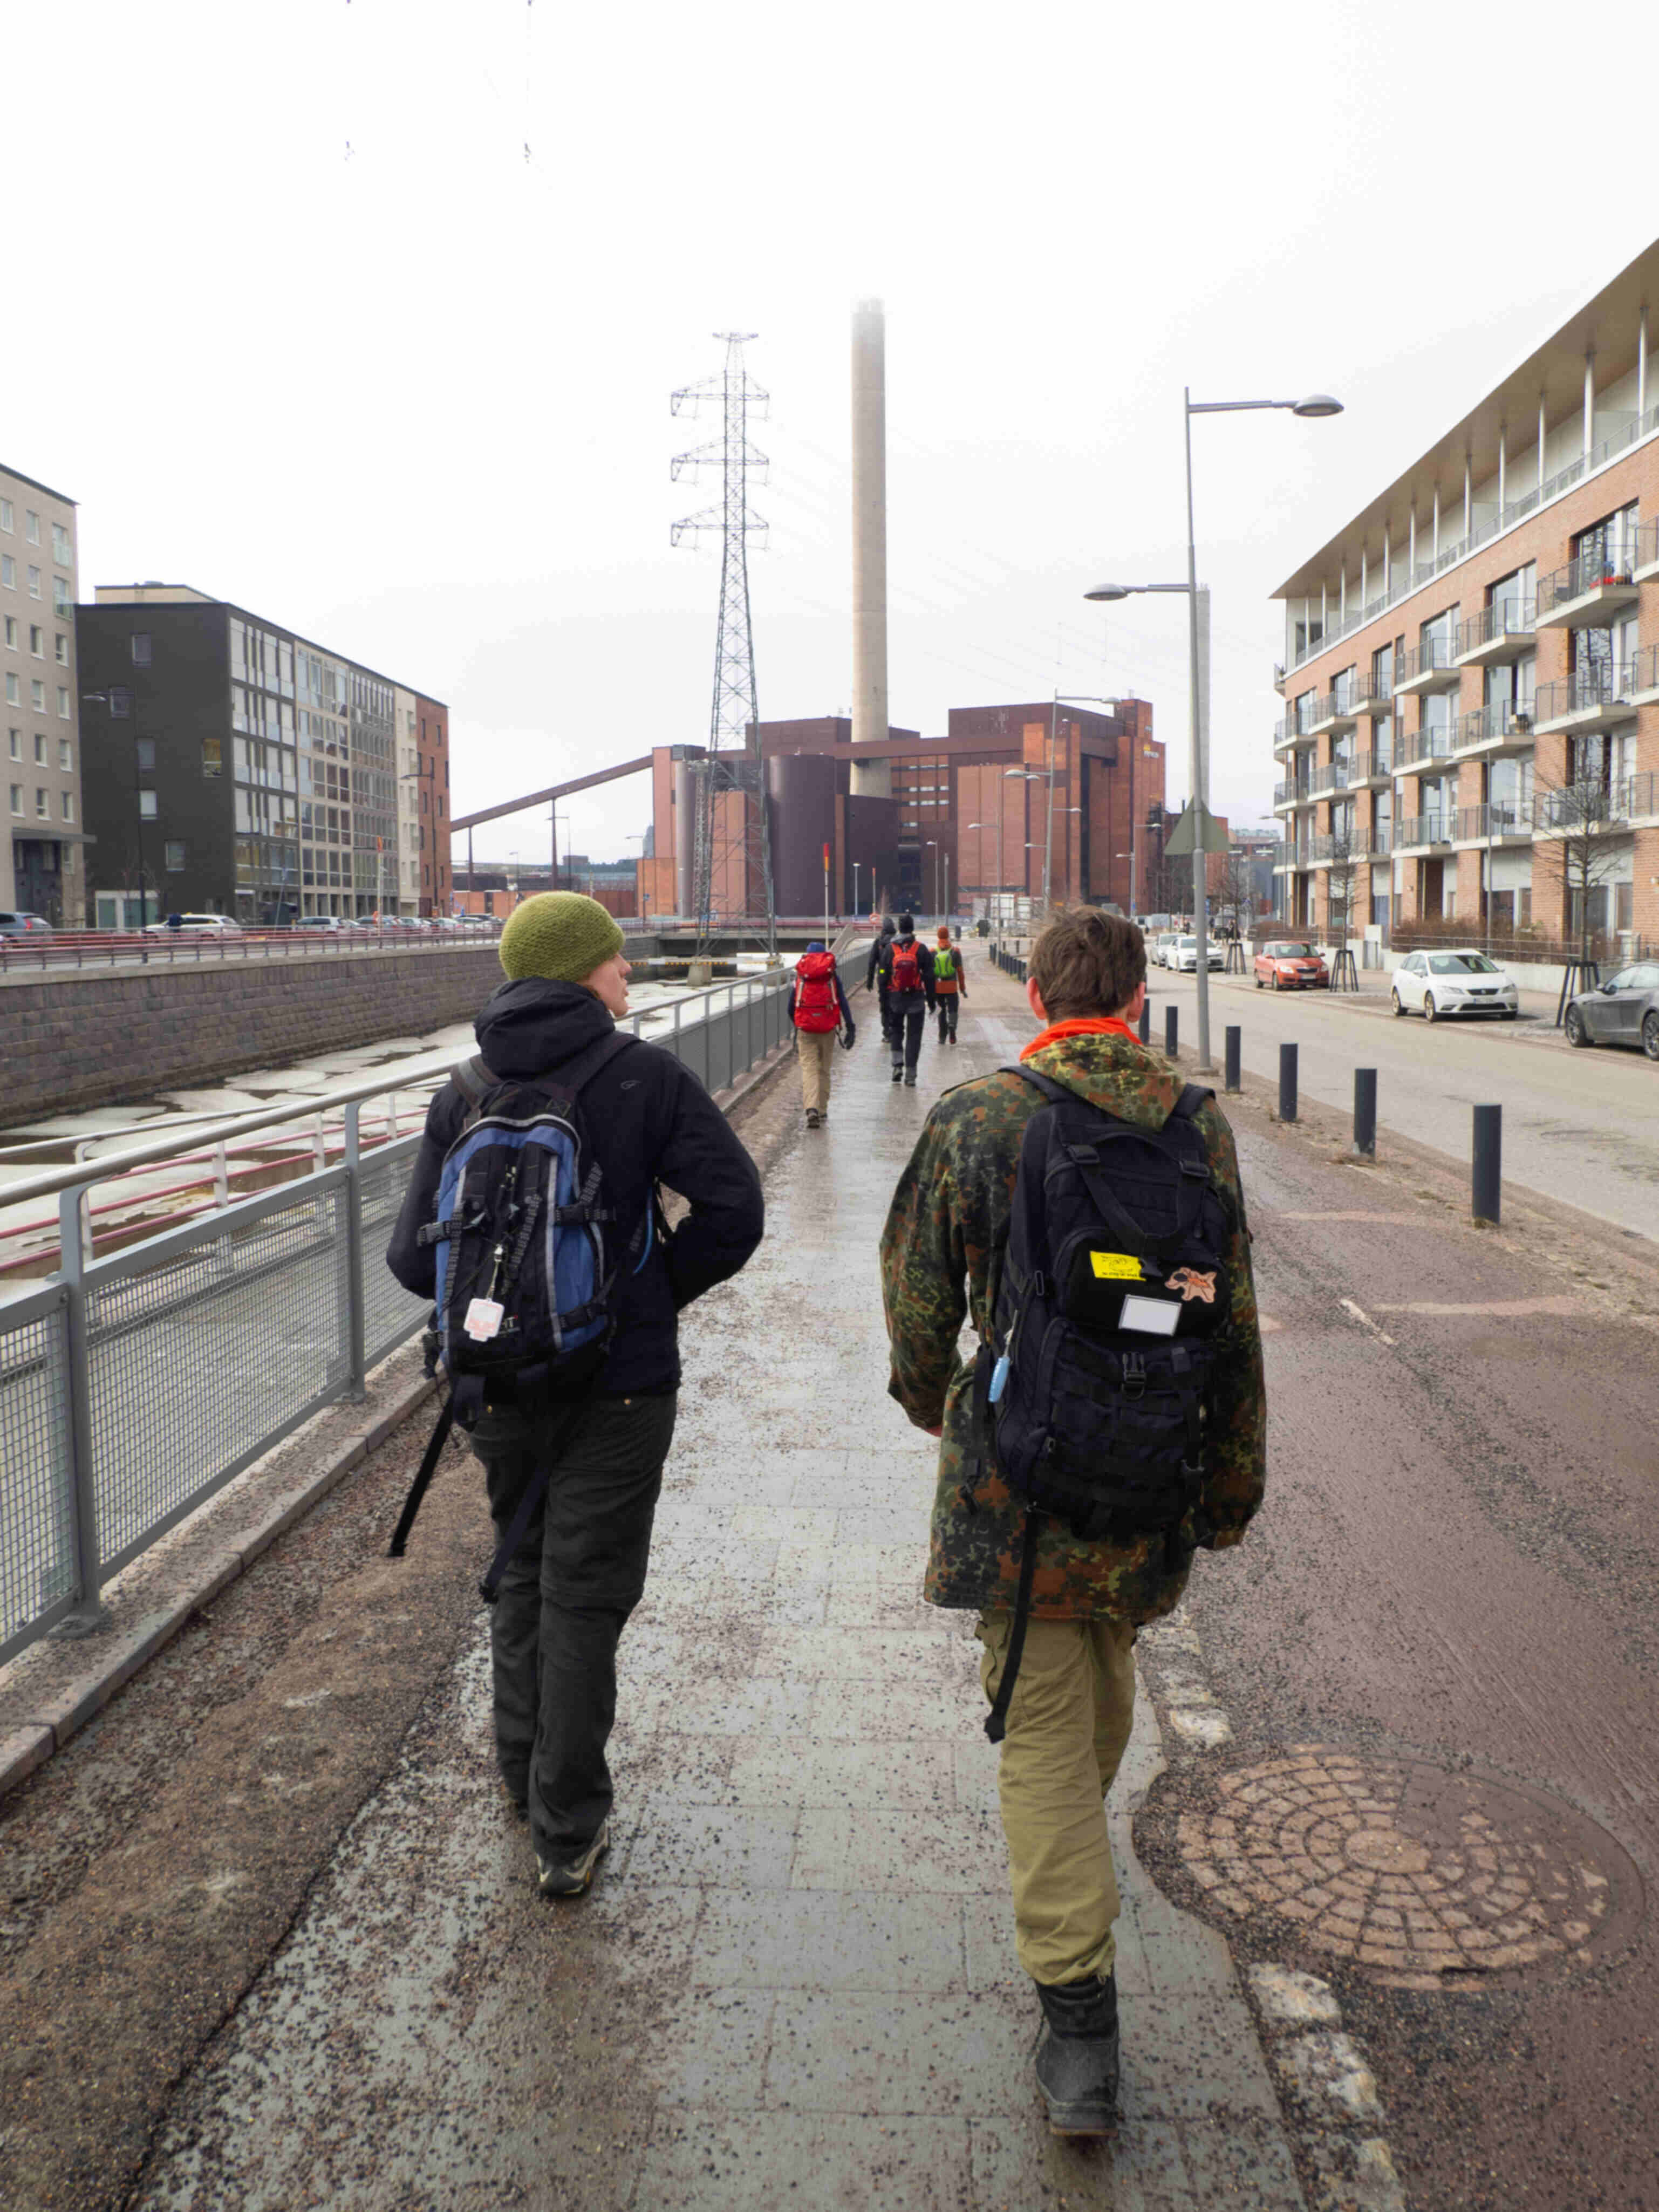
\includegraphics[width=\linewidth]{assets/nahkaliljakalasatama}

	Hakaniemen läpi päästiin juuri ja juuri jo mainitun liikennehankkeen
	työmaiden välistä pujotellen. Seureen etenemisvauhtia kuvasi hyvin
	Mikon kommentti, kuinka kukaan ei ollut vielä onnistunut vaeltajia
	ohittamaan. Kaisantunneli ei ollut ehtinyt vielä valmistua, mutta
	onneksi Linnunlaulun silta sai seurueen junaratojen länsipuolelle.
	Hakasalmen puistossa Töölönlahden rannalla Janne ja Tanguy nauttivat
	mämmiä \textbf{kello 15.44}. Kuivat sukat jalkaan ja vaellus jatkui.
	Jalkojen lisäksi myös nälkä alkoi painaa osaa vaeltajista. Linnuntietä
	maaliin oli yli kymmenen ja puoli kilometriä, mikä tarkoitti sitä, että
	vaadittu neljäkymmentä kilometriä tultaisiin todennäköisesti
	ylittämään.

	Töölönlahden kierron jälkeen suunta otettiin kohti maalia. Arvottiin,
	jahka oikaistaisiin takaisin Itäväylän vartta, mutta reittimestari
	pysyi vankasti reittisuunnitelmassaan. Sturenkatu ei tarjonnut
	erityisen kiinnostavaa maisemaa kävelylle, mutta Vallilan paahtimo
	herätti muistoja. Mäkelänkadun Subway tarjosi taktisen pysähdyksen,
	josta vauhtia sen enempää hidastamatta jatkettiin Arabianrantaan.

	\noindent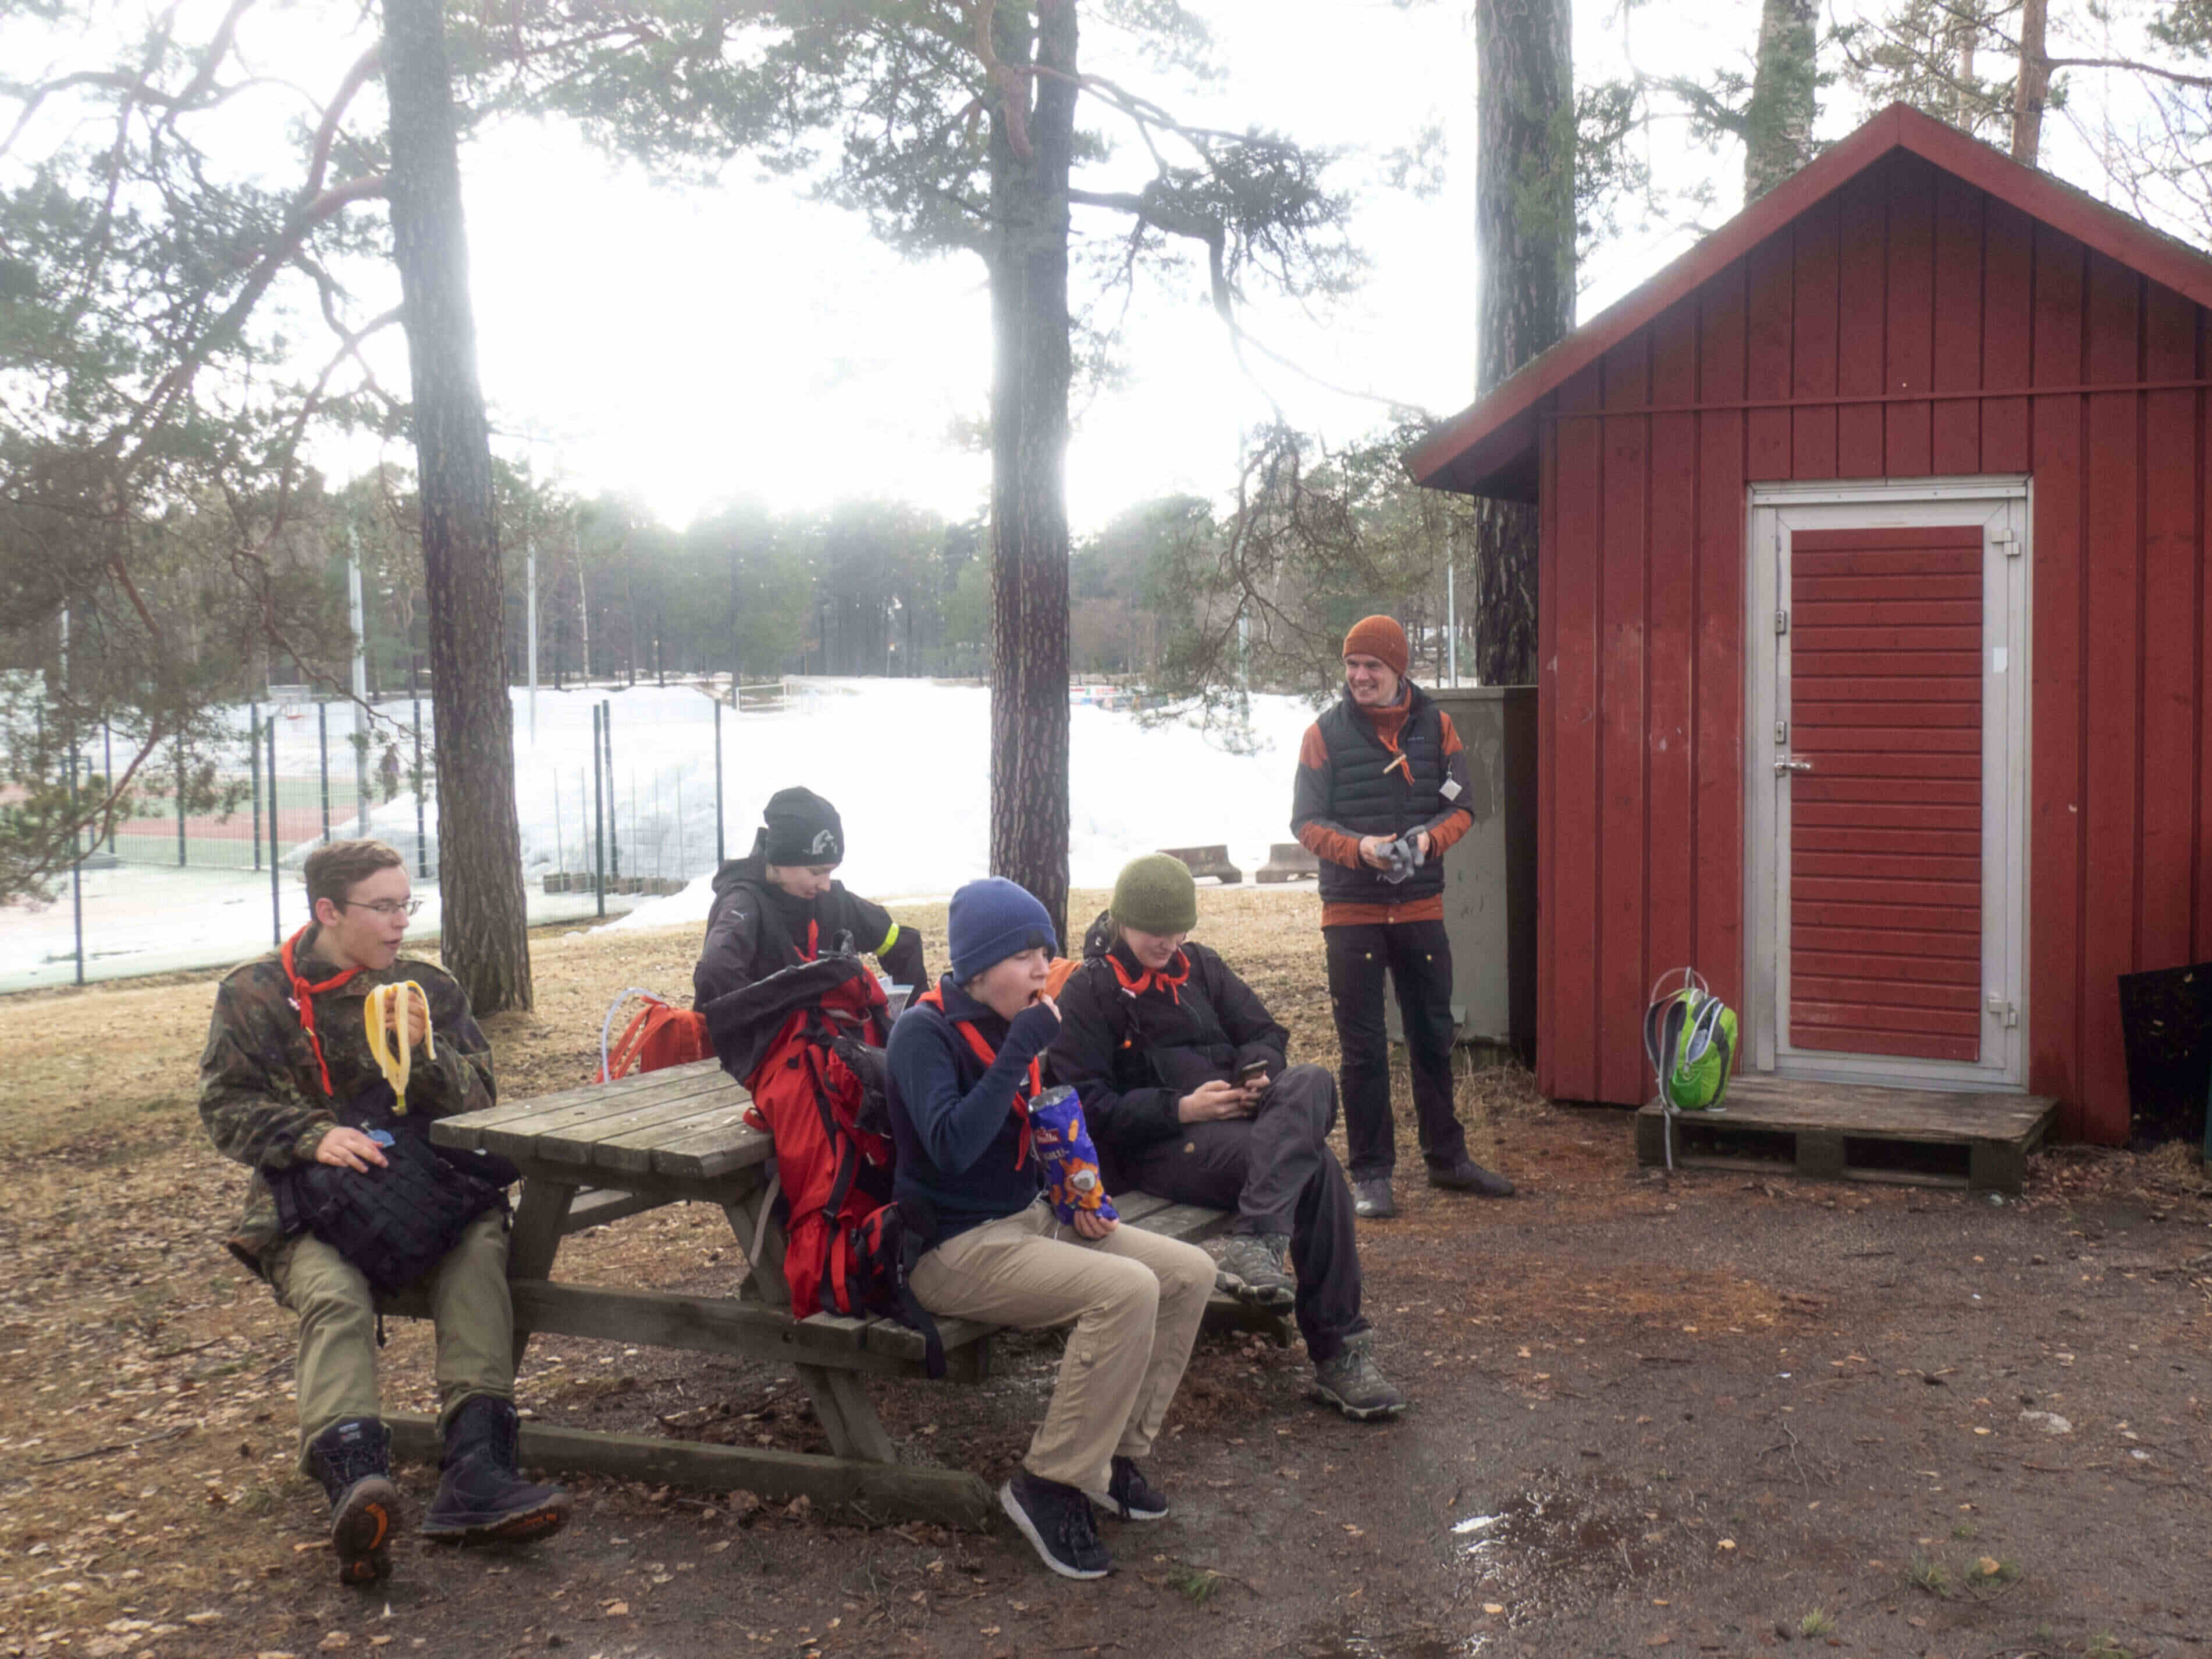
\includegraphics[width=\linewidth]{assets/nahkaliljamustikkamaa}

	Toukolan rantapuiston Laituri-ympäristötaideteos – tarkemmin,
	kuvataiteilija Merja Salosen laituri, jossa "näkyvät lapsuusmuistona
	mummolan järven hiekkapohjan aaltokuviot" – tarjosi seurueelle
	hengähdystauon ja istumapaikan \textbf{kello 17.01}. Tauon aikana muuan
	Toimen Tytöt -partiolippukunnan jäsen tuli ihmettelemään rusakoiden
	oransseja huiveja ja kertomaan, kuinka heidän partio-ohjelmansa
	riihityksessä oltiin hiihdetty kymmeniä kilometrejä vaikeakulkuisen
	puistikon läpi. (Toim. huom. TT muutti Töölöstä Arabianrantaan vuonna
	2008.) Tauko päättyi \textbf{kello 17.22}.

	Arvioitaessa Vanhankaupunginkosken ylitystä päädyttiin lyhimpään ja
	nopeimpaan ratkaisuun ylitettävien siltojen lukumäärän kustannuksella.
	Tässä vaiheessa vaeltajien välimatkat jo kasvoivat merkittävästi
	toisten jalkojen painaessa enemmän kuin toisten.

	Viikinportinkadun risteyksessä arvioitiin uudelleen nopeinta
	mahdollista reittiä maaliin, mutta jälleen reittimestari pysyi vankasti
	etukäteen valmistellussa reitissä. Tähän mennessä alkuperäinen
	taukostrategia oli riekaleina niin taukojen välimatkojen kuin niiden
	kestonkin suhteen; seuraava tauko pidettiin Viikintien varressa
	luonnonsuojelualueen kulmassa \textbf{kello 18.02}, jossa levättiin jo
	kevyenliikenteenväylällä maaten.

	Seurasi reitin tylsin osuus, Viikin suora, jolla itse kukin tunsi tai
	ei tuntenut jaloissaan aivan uusia tuntemuksia. Viikintieltä käänyttiin
	kohti Hallainvuorta ja Ilmolanraitilla pidettiin tauko \textbf{kello
	18.35}. Osallistujien mittarit näyttivät tässä vaiheessa neljänkymmenen
	kilometrin jo täyttyneen. Lippukunnan kolo oli jo kivenheiton päässä.
	Liukastelua vanhalla latupohjalla ja pian oltiin jo tutussa ja
	turvallisessa Kivikossa, kun seurue ylitti Kehä I:n Viikinpuistonsiltaa
	pitkin.

	Kivikon puolella pohdittiin, sikäli mikäli maaliin olisi välttämätöntä
	kaikkien kävellä, koska määritelty matka oli mitä todennäköisimmin jo
	saatu täyteen. Niinpä Elias erkani seurueesta kotimatkalle
	Kivikonlaidan varrella \textbf{kello 18.59}, Tanguy ja Toivo jäivät
	Kivijatatien bussipysäkille \textbf{kello 19.06} ja Leon autokyyti otti
	hänet mukaansa Panosaukion tuntumasta \textbf{kello 19.09}.

	\begin{center}
	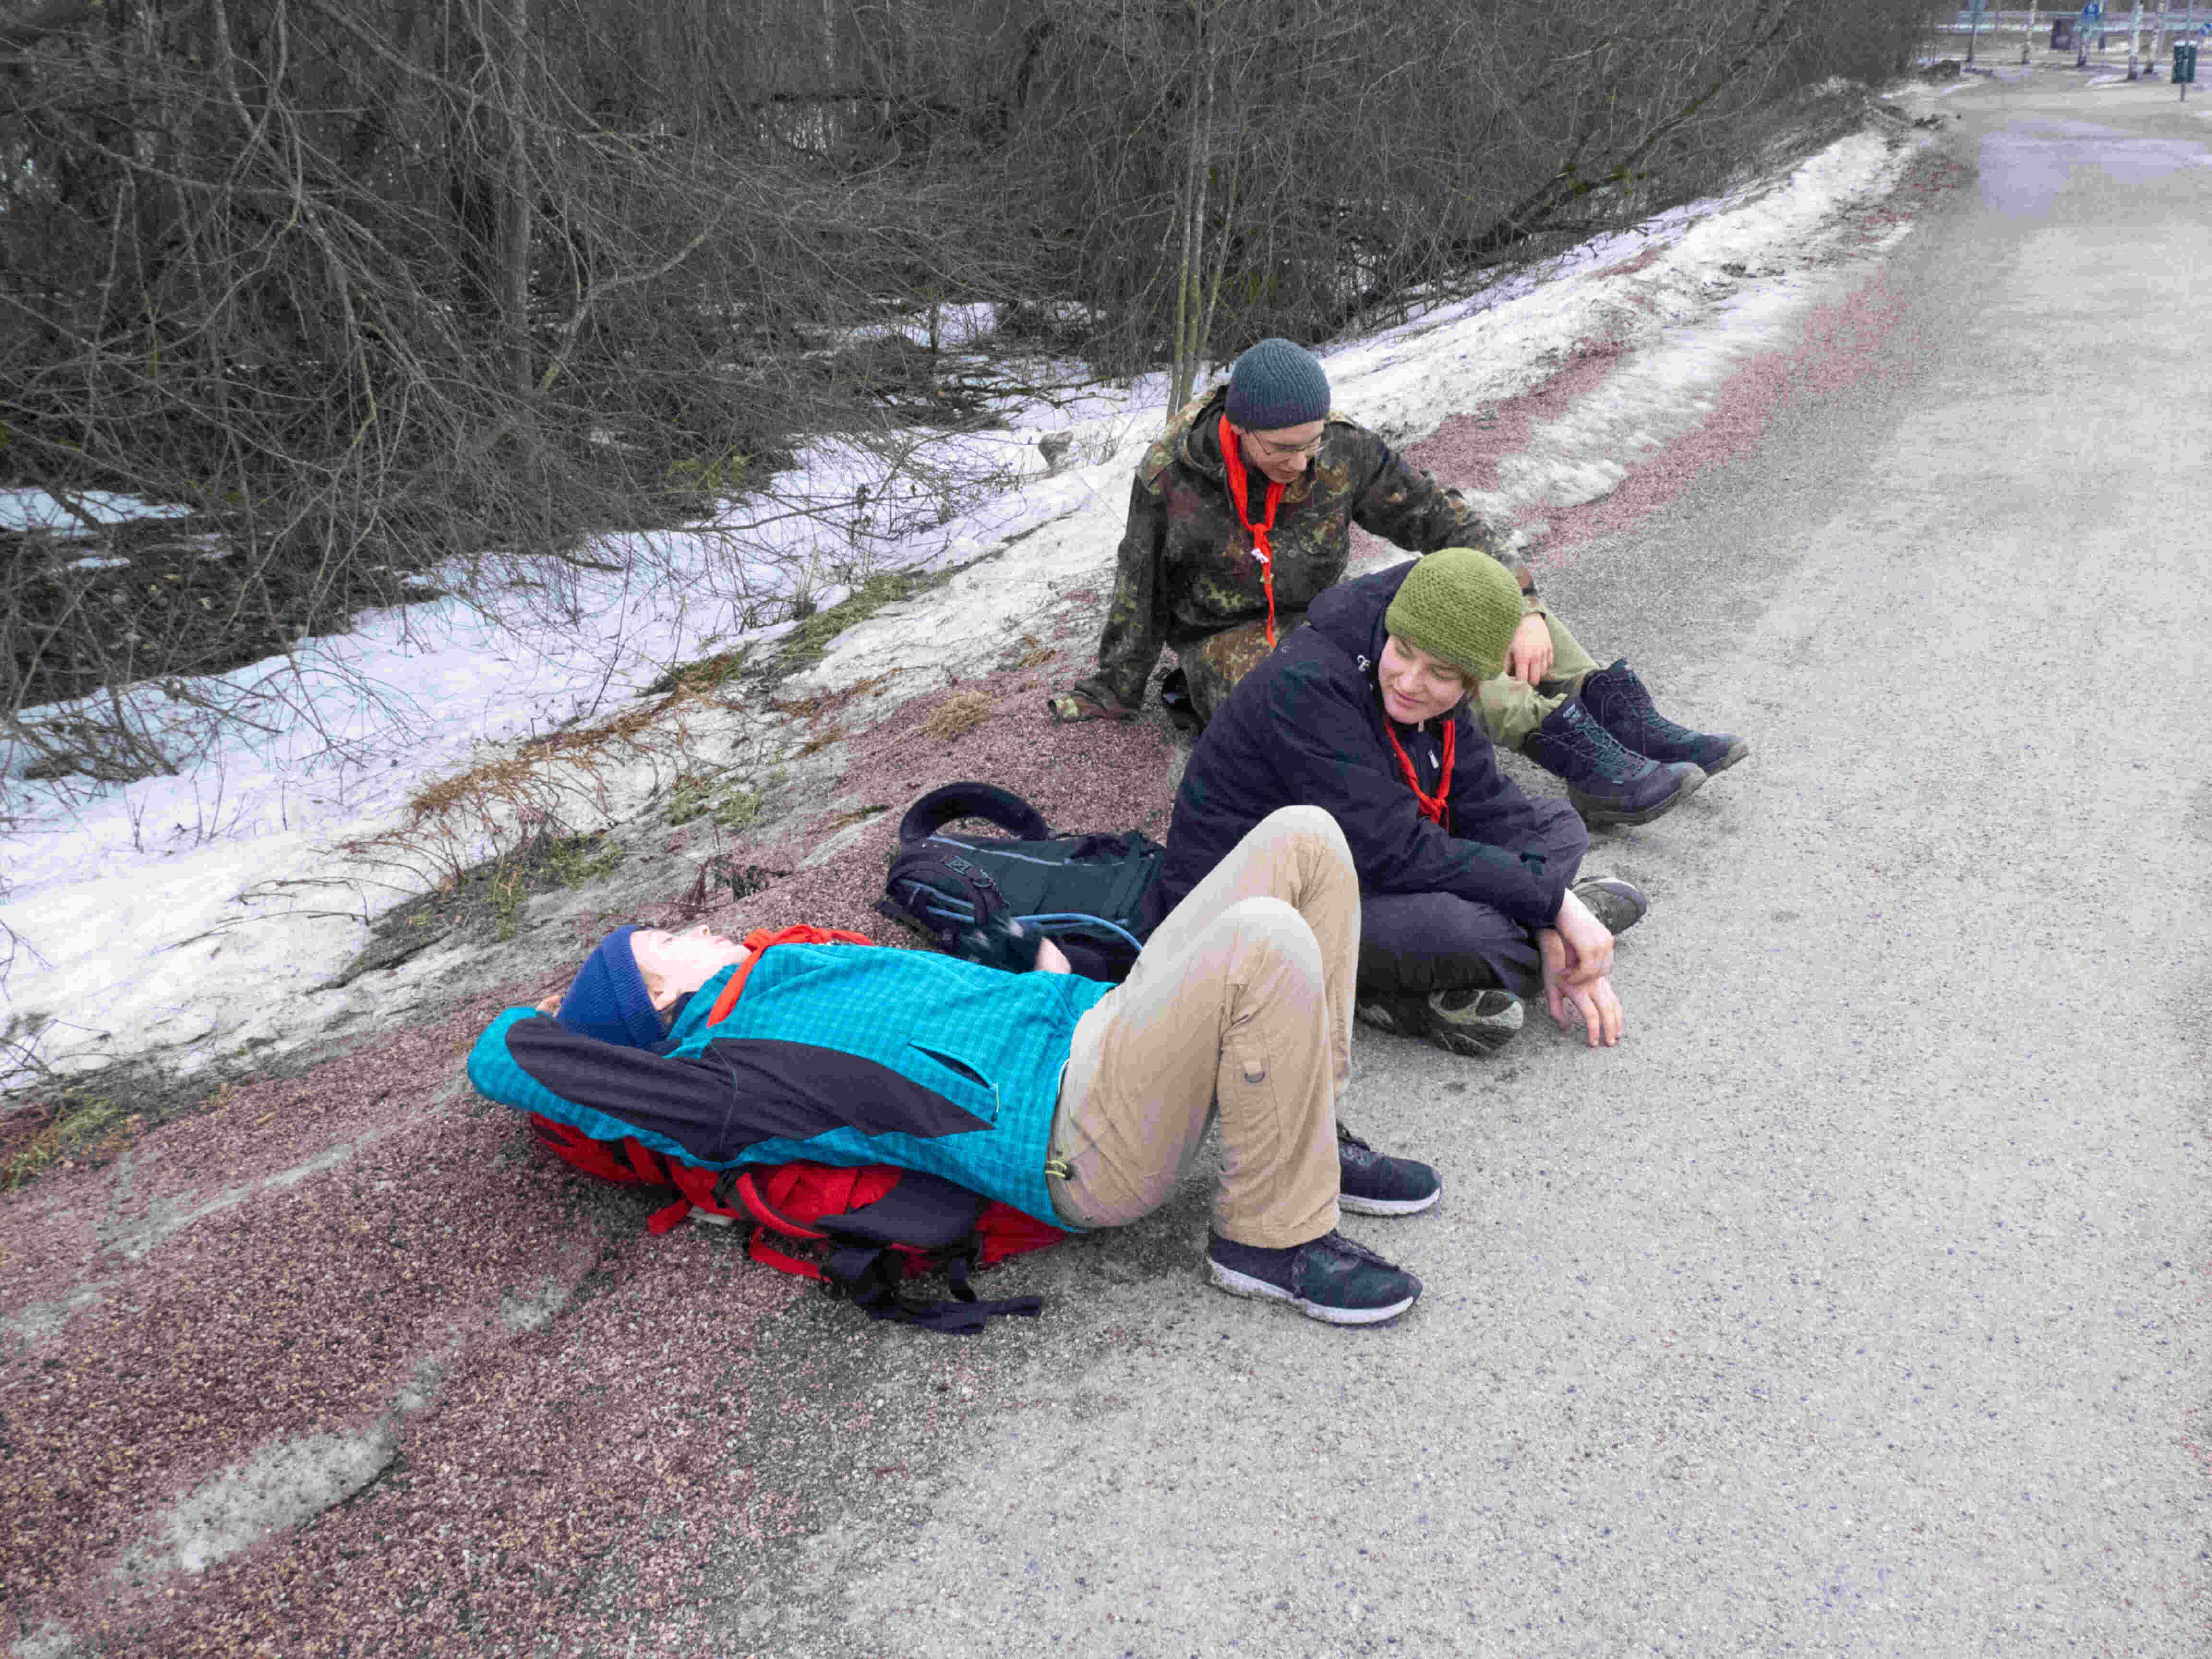
\includegraphics[width=\linewidth]{assets/nahkaliljaviikki}
	\end{center}

	Jäljelle jääneet vaeltajat Ahti, Janne ja Mikko kävelivät maaliin asti,
	jossa he olivat reittimestarin kellon mukaan \textbf{kello 19.32}. Koko
	matkan pituudeksi tuli tarkistusmittauksen jälkeen reilu
	neljäkymmentäkolme kilometriä, mikä tarkoitti noin 4,2 kilometrin
	tuntivauhtia – todella haipakkaa siis. Punaisen nahkaliljan
	viisikymmentä kilometriä ei siis ole haaste eikä mikään!

	Ilmatieteen laitoksen Kumpulan havaintoasemalla merkittiin
	vaelluspäivän sääksi puolipilvisestä pilviseen, lämpötila 2–5 astetta,
	länsituulta 3–7 metriä sekunnissa ja ilmankosteus 77–93 prosenttia –
	mitä erinomaisin nahkaliljakeli, sanoisin!\\

	\vspace*{0.50cm}

	\raggedleft Kuvat: Tanguy Gérôme\\
	\raggedleft Teksti: Janne Suomalainen

\end{multicols}

% Lopuksi, tässä on jokaisen osallistujan kolmen sanan tiivistelmä.
% Valitettavasti, päätoimittaja sekoitti hänen muistiinpanonsa.
% Teillä on tehtävä: kuka sanoi mitä.

% \begin{center}
% 	\begin{tabular}{ |c||ccc||c| }
% 		\hline
% 		Ahti & a. & & 1. & hauska hyvä sää \\
% 		\hline
% 		Elias & b. & & 2. & jalat irtoavat pois \\
% 		\hline
% 		Janne & c. & & 3. & kipu kärsimys ruoka \\
% 		\hline
% 		Leo & d. & & 4. & minä pidän kävely \\
% 		\hline
% 		Mikko & e. & & 5. & mulla on nälkä \\
% 		\hline
% 		Tanguy & f. & & 6. & oli hauska aloituksessa \\
% 		\hline
% 		Toivo & g. & & 7. & optimaalinen reipas keväinen \\
% 		\hline

		% Ahti & a. & & 1. & hauska & hyvä & sää \\
		% \hline
		% Elias & b. & & 2. & jalat & irtoavat & pois \\
		% \hline
		% Janne & c. & & 3. & kipu & kärsimys & ruoka \\
		% \hline
		% Leo & d. & & 4. & minä & pidän & kävely \\
		% \hline
		% Mikko & e. & & 5. & mulla & on & nälkä \\
		% \hline
		% Tanguy & f. & & 6. & oli & hauska & aloituksessa \\
		% \hline
		% Toivo & g. & & 7. & optimaalinen & reipas & keväinen \\
		% \hline

		% Ahti & minä & pidän & kävely \\
		% \hline
		% Elias & mulla & on & nälkä \\
		% \hline
		% Janne & optimaalinen & reipas & keväinen \\
		% \hline
		% Leo & kipu & kärsimys & ruoka \\
		% \hline
		% Mikko & hauska & hyvä & sää \\
		% \hline
		% Tanguy & oli & hauska & aloituksessa \\
		% \hline
		% Toivo & jalat & irtoavat & pois \\
		% \hline

		% Ahti & minä pidän kävely \\
		% \hline
		% Elias & mulla on nälkä \\
		% \hline
		% Janne & optimaalinen reipas keväinen \\
		% \hline
		% Leo & kipu kärsymys ruoka \\
		% \hline
		% Mikko & hauska hyvä sää \\
		% \hline
		% Tanguy & oli hauska aloituksessa \\
		% \hline
		% Toivo & jalat irtoavat pois \\
		% \hline
	% \end{tabular}
% \end{center}



\section{Kolkkien ja seikkalijoiden päiväretki 13.4.}

% \vspace*{-0.16cm}
\begin{center}
	\noindent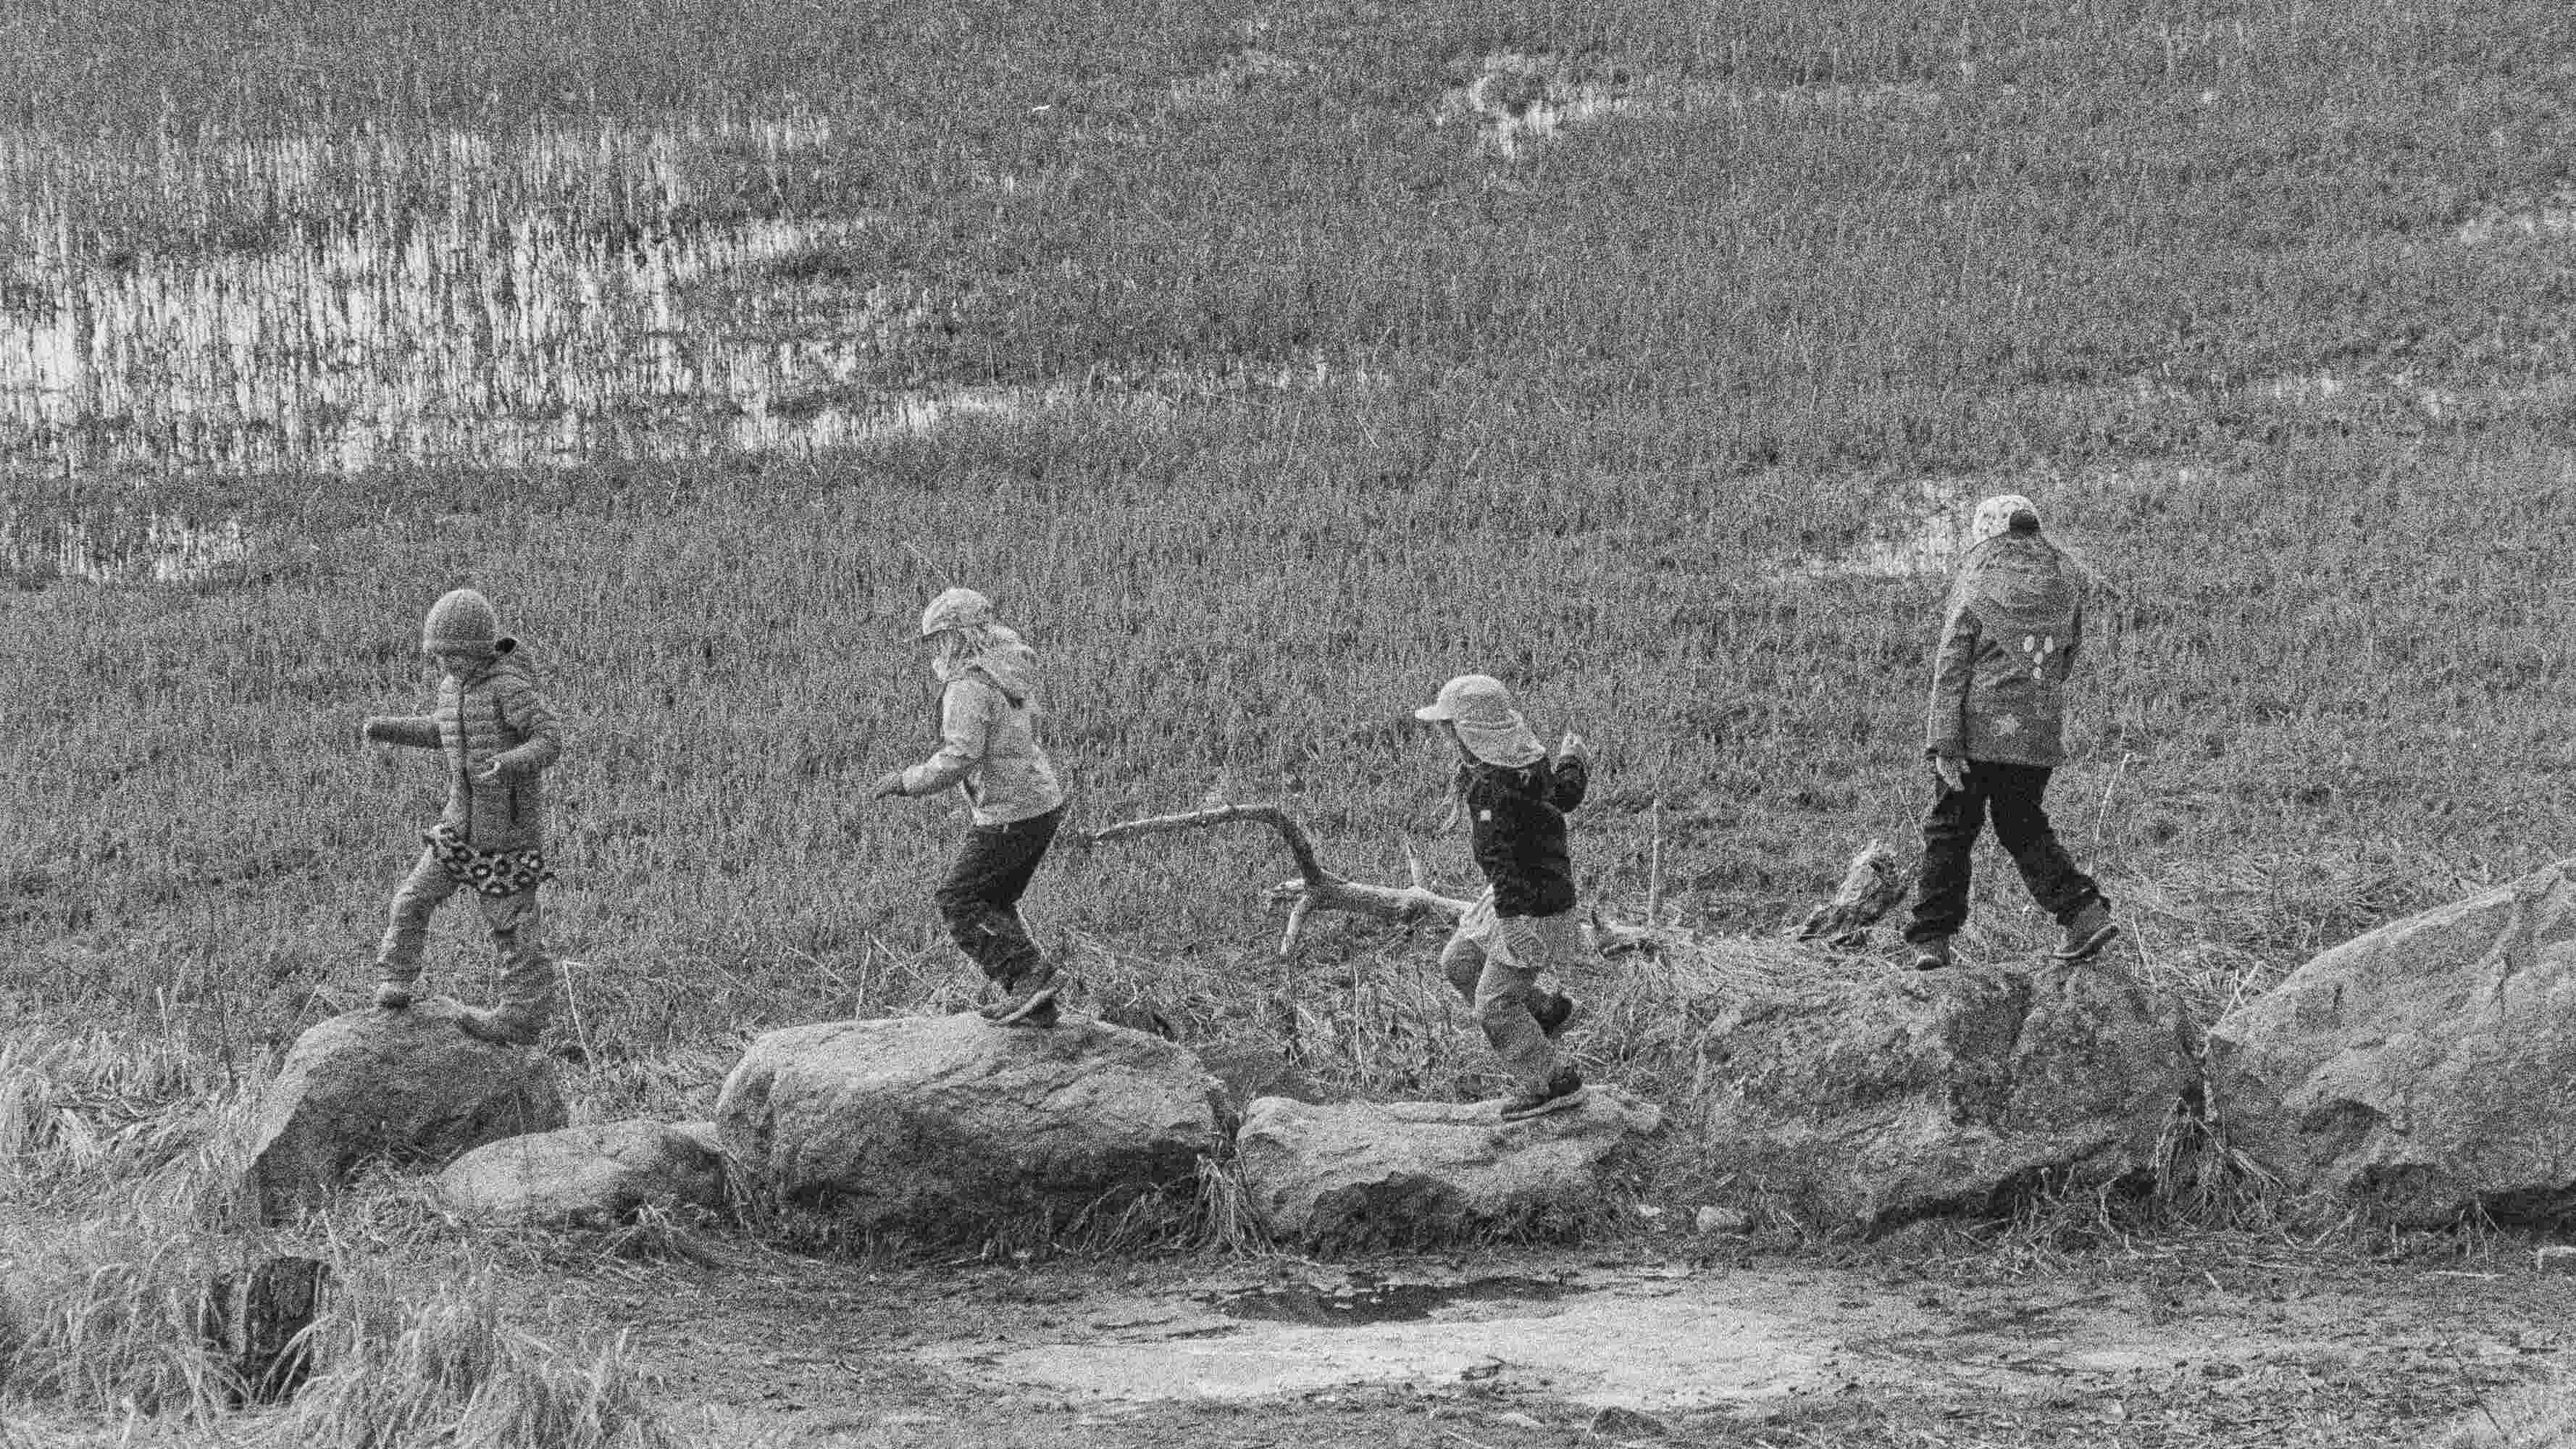
\includegraphics[width=0.8\linewidth]{assets/kolkkienpäiväretkibw3}
\end{center}
\vspace*{-0.16cm}

\begin{multicols}{2}

	\noindent Lippukunnan kolkat ja seikkailijat tekivät yhteisen päiväretken
	huhtikuisena lauantaina. Retkue kokoontui ohjeistetusti Kivikossa
	Järkälekujan bussipysäkillä, jonne Alisa, Annina, Elna, Janja, Janne,
	Johannes, Kuisma, Lillian, Nella, Sade, Tanguy ja Veera (harmillisesti
	ainoa retkelle ilmoittautunut seikkailija oli sairastunut) saapuivat
	kaikki niin hyvissä ajoin, että retkue pääsi suunniteltua aikaisemman
	bussin kyytiin – mitä nyt muutamaa kolkkaa piti kiiruhtaa lopettamaan
	terveysaseman kallioilla kiipeileminen.

	Bussista jäätiin Latokartanon pysäkillä, josta käveltiin reippaasti
	entisen puutarhan, nykyisen olutpanimon läheiselle parkkipaikalle.
	Parkkipaikalle olivatkin juuri parahiksi saapuneet myös Ilona, Jella,
	Leo ja Nonna, joiden autosta otettiin kantoon vesi ja tiskivadit.
	\mbox{Retki Viikinrannan} kevätluontoon voi \mbox{alkaa!}

	Pari sataa metriä myöhemmin jo pysähdyttiin entisen maatalousmuseon
	edessä ihmettelemään puuhun kiinnitettyä ohjeistusta:
	Pistelaskentapaikka Jyväskylän yliopistossa kehitetylle Muuttolintujen
	Kevät -mobiilisovellukselle, jonka "avulla sinulla on mahdollisuus
	tallentaa linnunlaulua ja tehdä lintuhavaintoja hyödyntäen modernia
	tekoälyä". Pikemmittä puheitta retkenjohtaja Annina otti puhelimen
	esiin ja aloitti viiden minuutin mittauksen, jonka aikana tuli olla
	aivan hiljaa. Vaikka viisi minuuttia tuntui ehkä joistakuista
	ikuisuudelta, meni aika kuitenkin nopeasti ilman ylimääräistä
	metelöintiä luonnon ääniä kuunnellen.

	\columnbreak

	(Toim. huom. havaintoaineisto on avointa ja löytyy valmiiksi kartalta
	esimerkiksi täältä:
	\href{https://yle.fi/aihe/a/20-10004726}{https://yle.fi/aihe/a/20-10004726}.
	Retken laskentapaikalle on merkitty 13.4. kalalokki, kuovi,
	sepelkyyhky, talitiainen ja varis – osa mahdollisesti meidän tekemän
	mittauksen ansiosta! Sunnuntaihin 14.4. mennessä sovelluksella oli
	kerätty yli kolme miljoonaa äänitystä Helsingissä ja Jyväskylässä
	tutkijoiden käyttöön.)

	Hiljaisuusharjoituksen jälkeen jatkettiin kohti Keinumäen lintutornia,
	jonka läheisyydessä oli määrä laittaa lounasta – kolkat kun suorittivat
	keväällä retkikokki-jälkeä. Viikin puupuiston tietämillä Tanguy
	ohjeisti retkeläisille lintubingon, jossa merkinnän ruudukkoon sai
	tehdä esimerkiksi linnun keltaisesta nokasta, uivasta linnusta ja
	laulavasta talitiaisesta. Ensimmäinen bingo saatiin jo ennen Keinumäkeä
	ja palkittiin asianmukaisesti rusinoilla.

	\begin{Figure}
		\noindent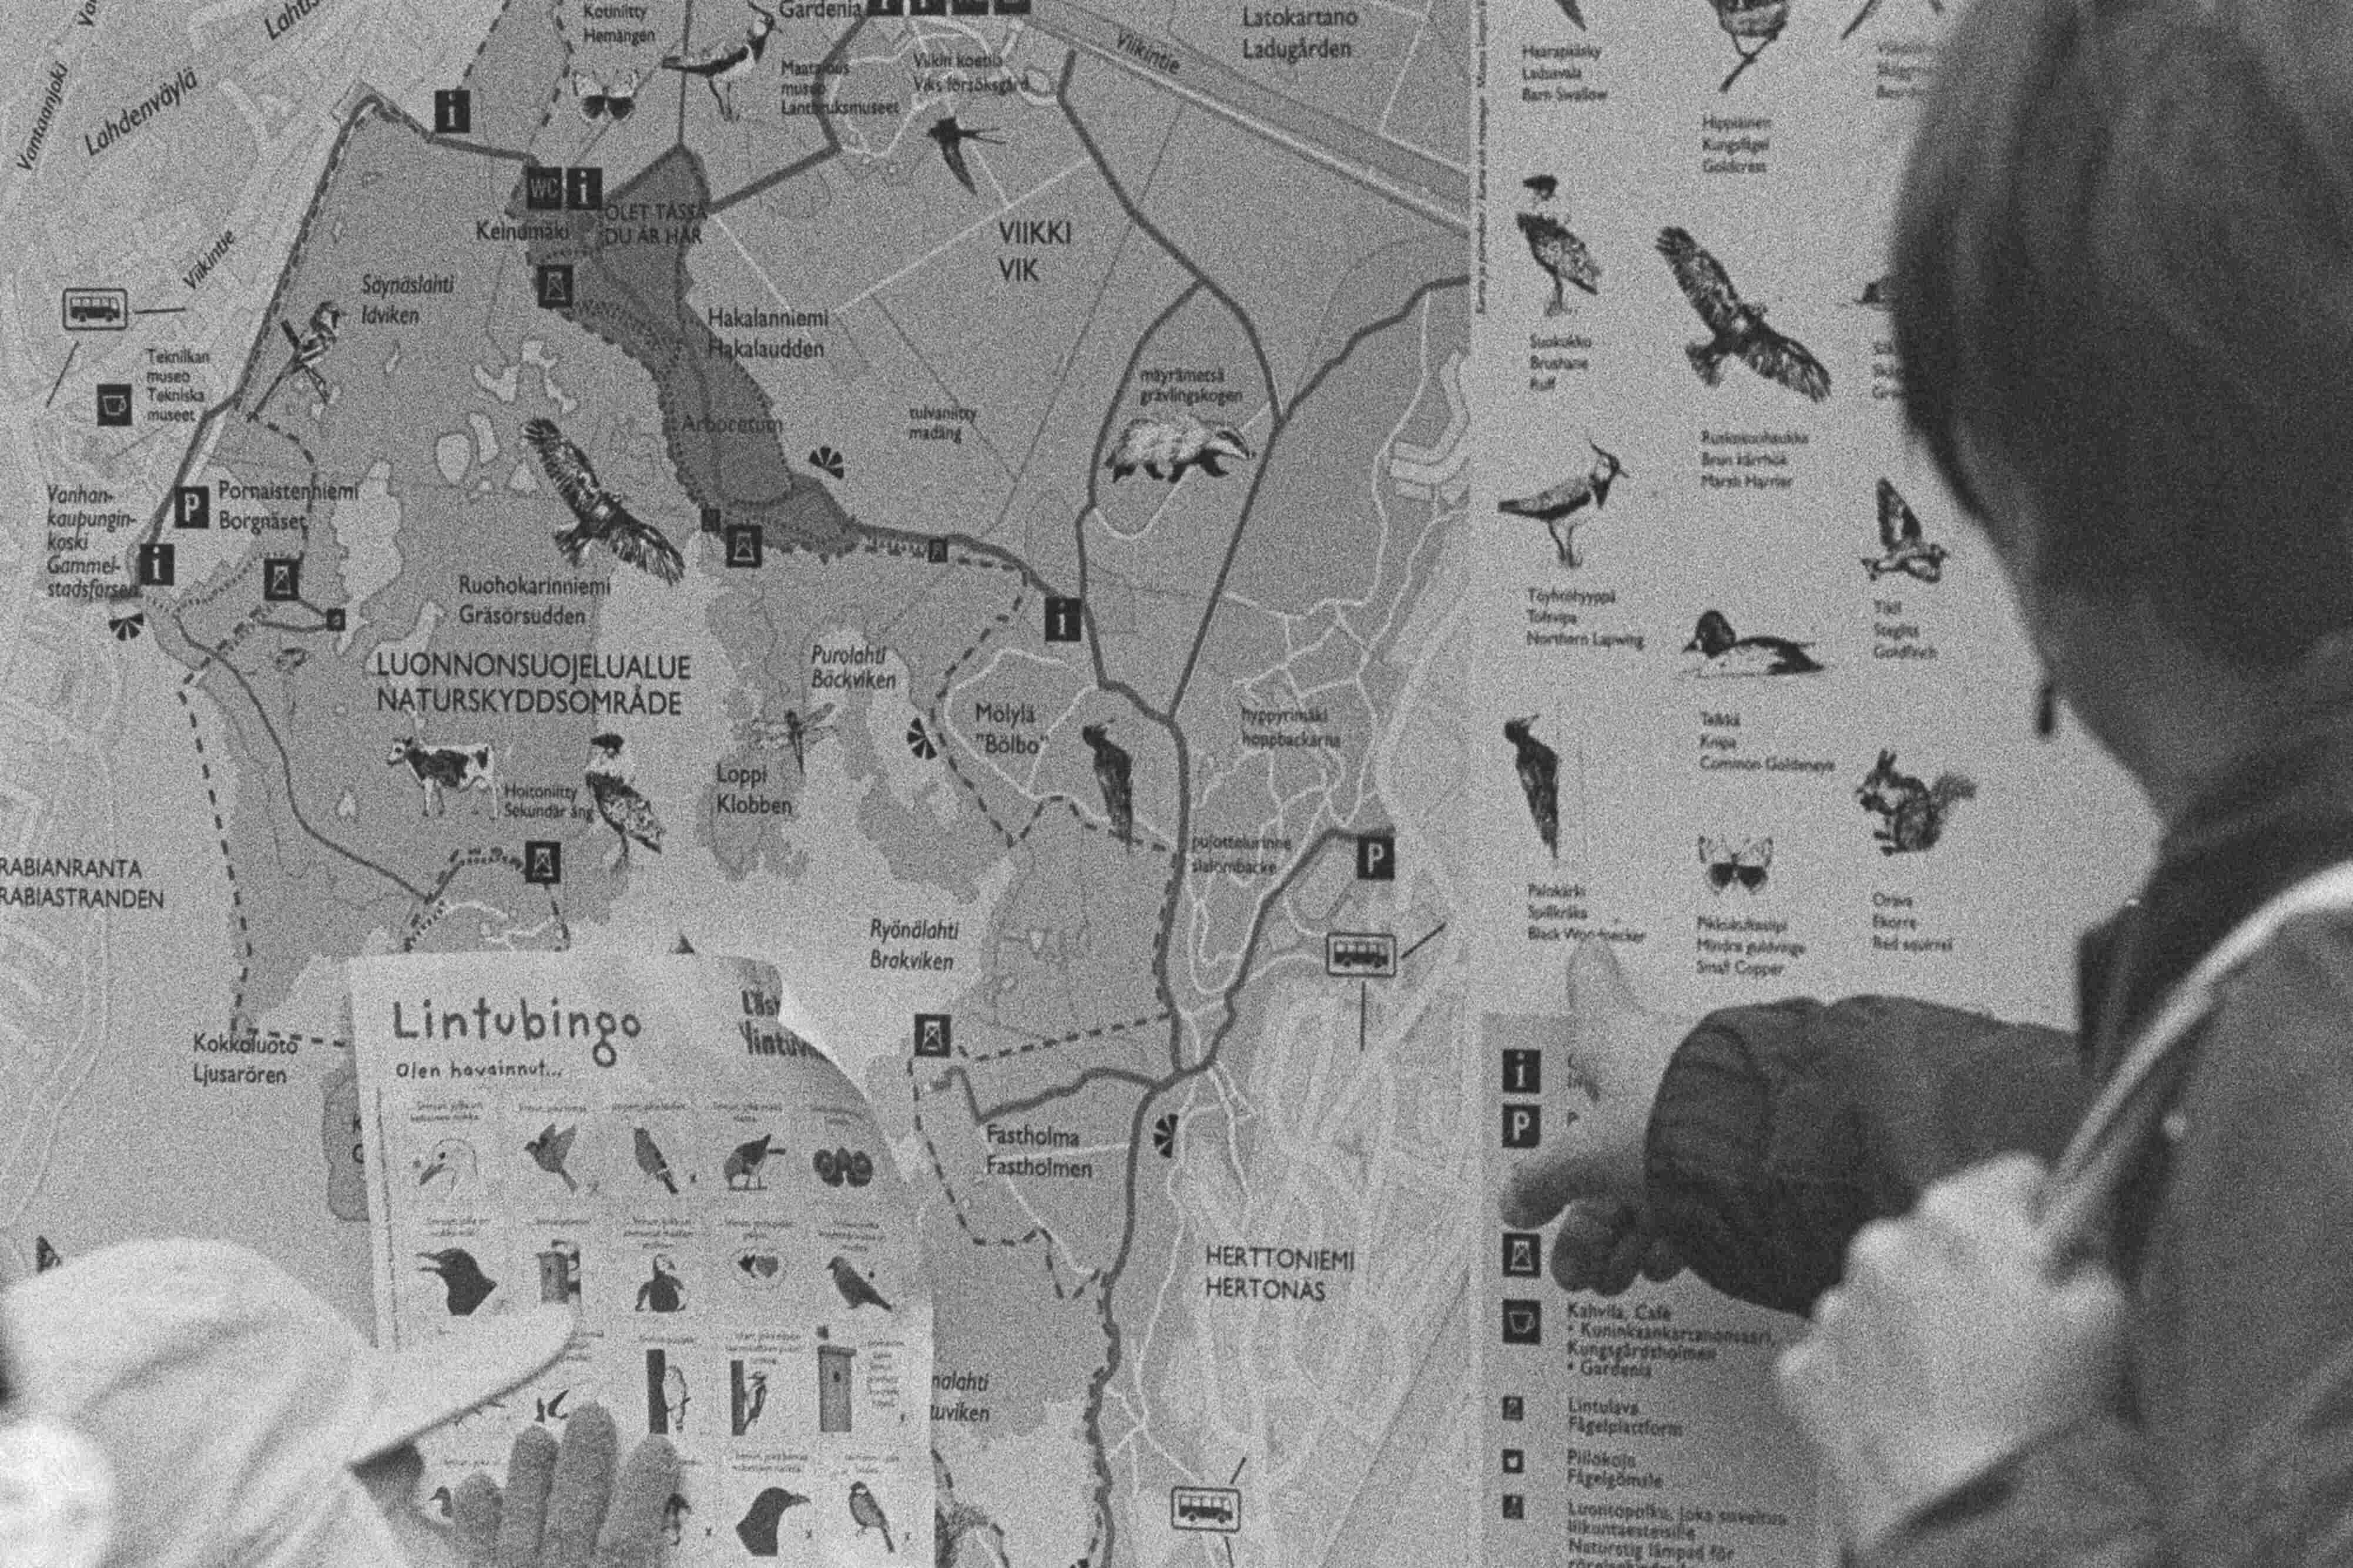
\includegraphics[width=\linewidth]{assets/kolkkienpäiväretkibw1}
	\end{Figure}

	Lyhyt pysähdys opastauluilla ja oltiin jo lintutornilla. Trangiat
	kaivettiin esiin ja aloitettiin ruoanvalmistus; kolkat olivat
	suunnitelleet retkelle kahden ruokalajin aterian valmiiksi kevään
	kokouksissaan. Pääruoaksi oli vegaanista nakkikeittoa ja jälkiruoaksi
	kaura-omenapaistosta vaniljakastikkeella. Keitto valmistui varsin
	jouhevasti, vaikka jotkut retkeläiset olivatkin innokkaammin
	leikkimässä kuin leikkaamassa nakkeja ja omenoita. Veden kiehumista
	odotellessa halukkaat pääsivät myös kiipeämään lintutorniin seuraamaan
	lintuja Vanhankaupunginlahdella. Kevätmuutto oli vasta aluillaan, minkä
	vuoksi lintuja ei havaittu aivan yhtä paljon kuin BirdLife Suomen
	Tornien taisto -kilpailussa vuonna 2023 (102 lintulajia/8 tuntia).

	% \vspace*{-0.32cm}
	\begin{center}
		\noindent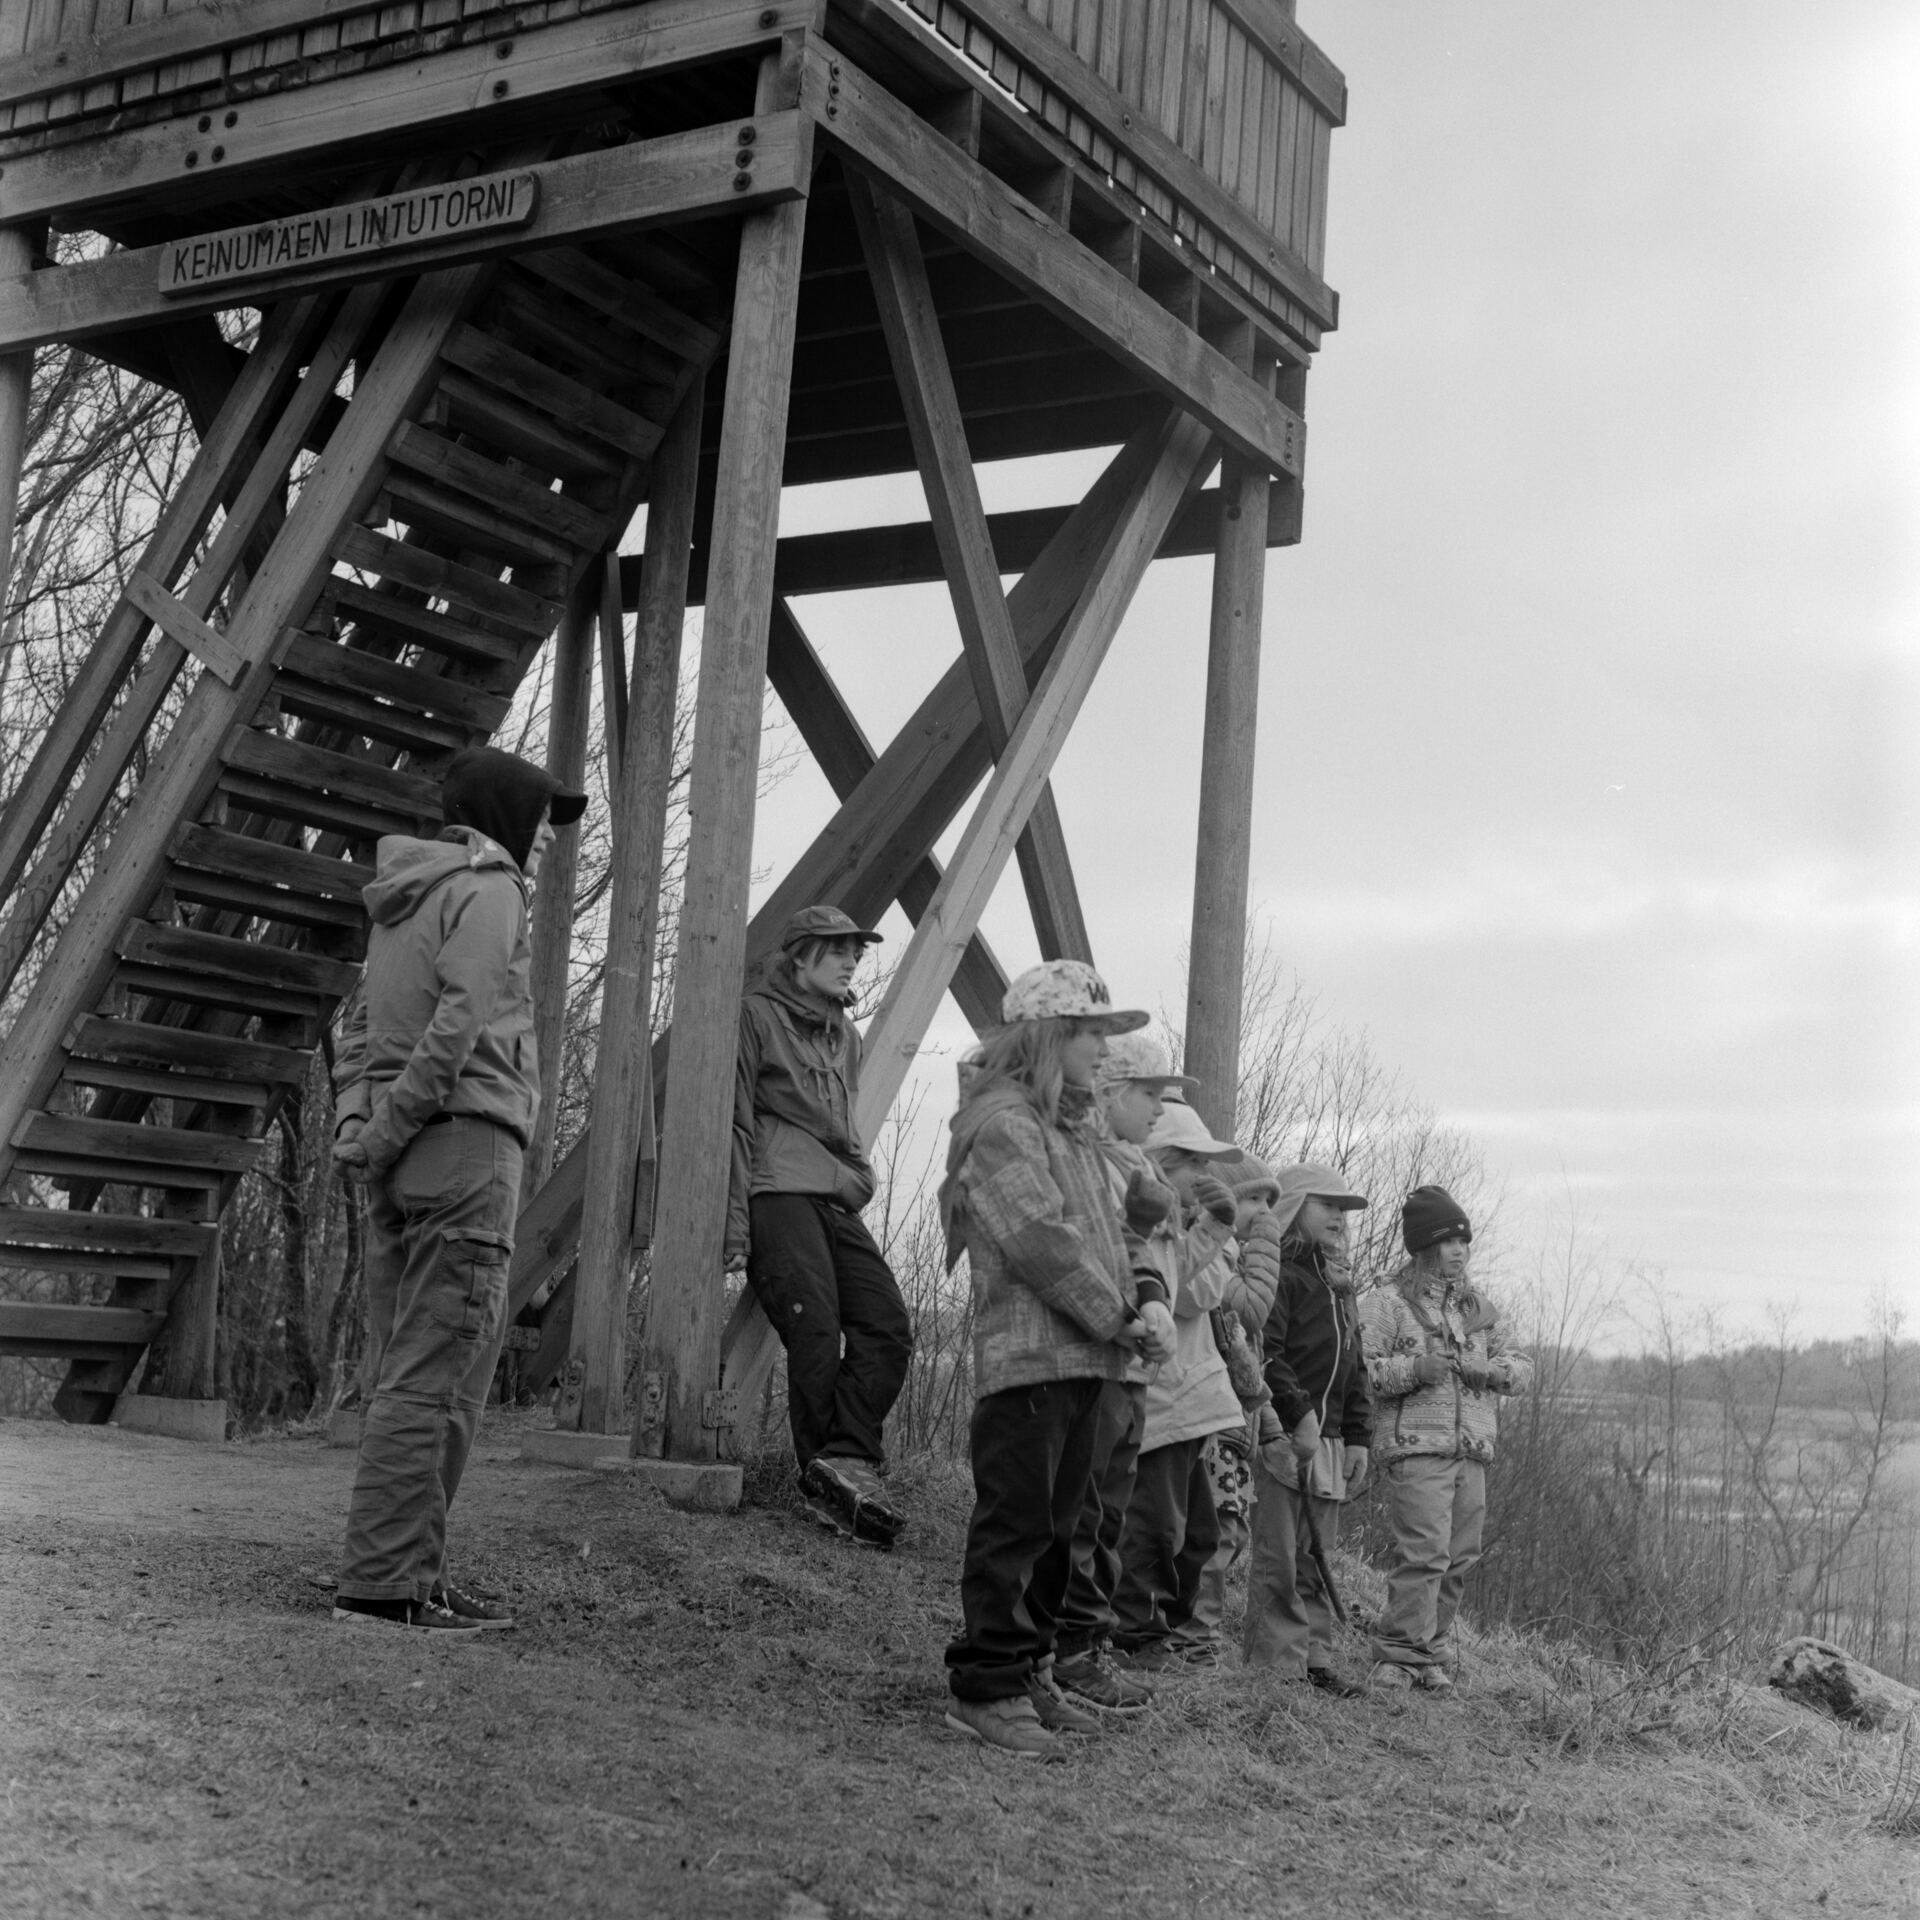
\includegraphics[width=0.8\linewidth]{assets/kolkkienpäiväretkibw15}
	\end{center}

	Keittojuuresten kiehuessa nälkä alkoi jo kurnimaan ja viimein saatiin
	oikein herkullista keittoa – lämmikkeeksi sulan meren yli puhaltaneen
	tuulen jäähdyttämille retkeilijöille. Onneksi jälkiruoka valmistui
	nopeammin. Paistosta oltiin koeajettu kolkkien kokouksessa jo
	aikaisemmin keväällä ja suurta makunautintoa kannatti odottaa. Retken
	alkupään viiden minuutin mittainen hiljaisuus oli tässä vaiheessa
	muuttunut jo hataraksi muistikuvaksi, kun retkeläisten äänenkäyttö
	hipoi häiritsevän voimakasta meteliä. 

	% \columnbreak

	% \vspace*{-0.64cm}
	\begin{center}
		\noindent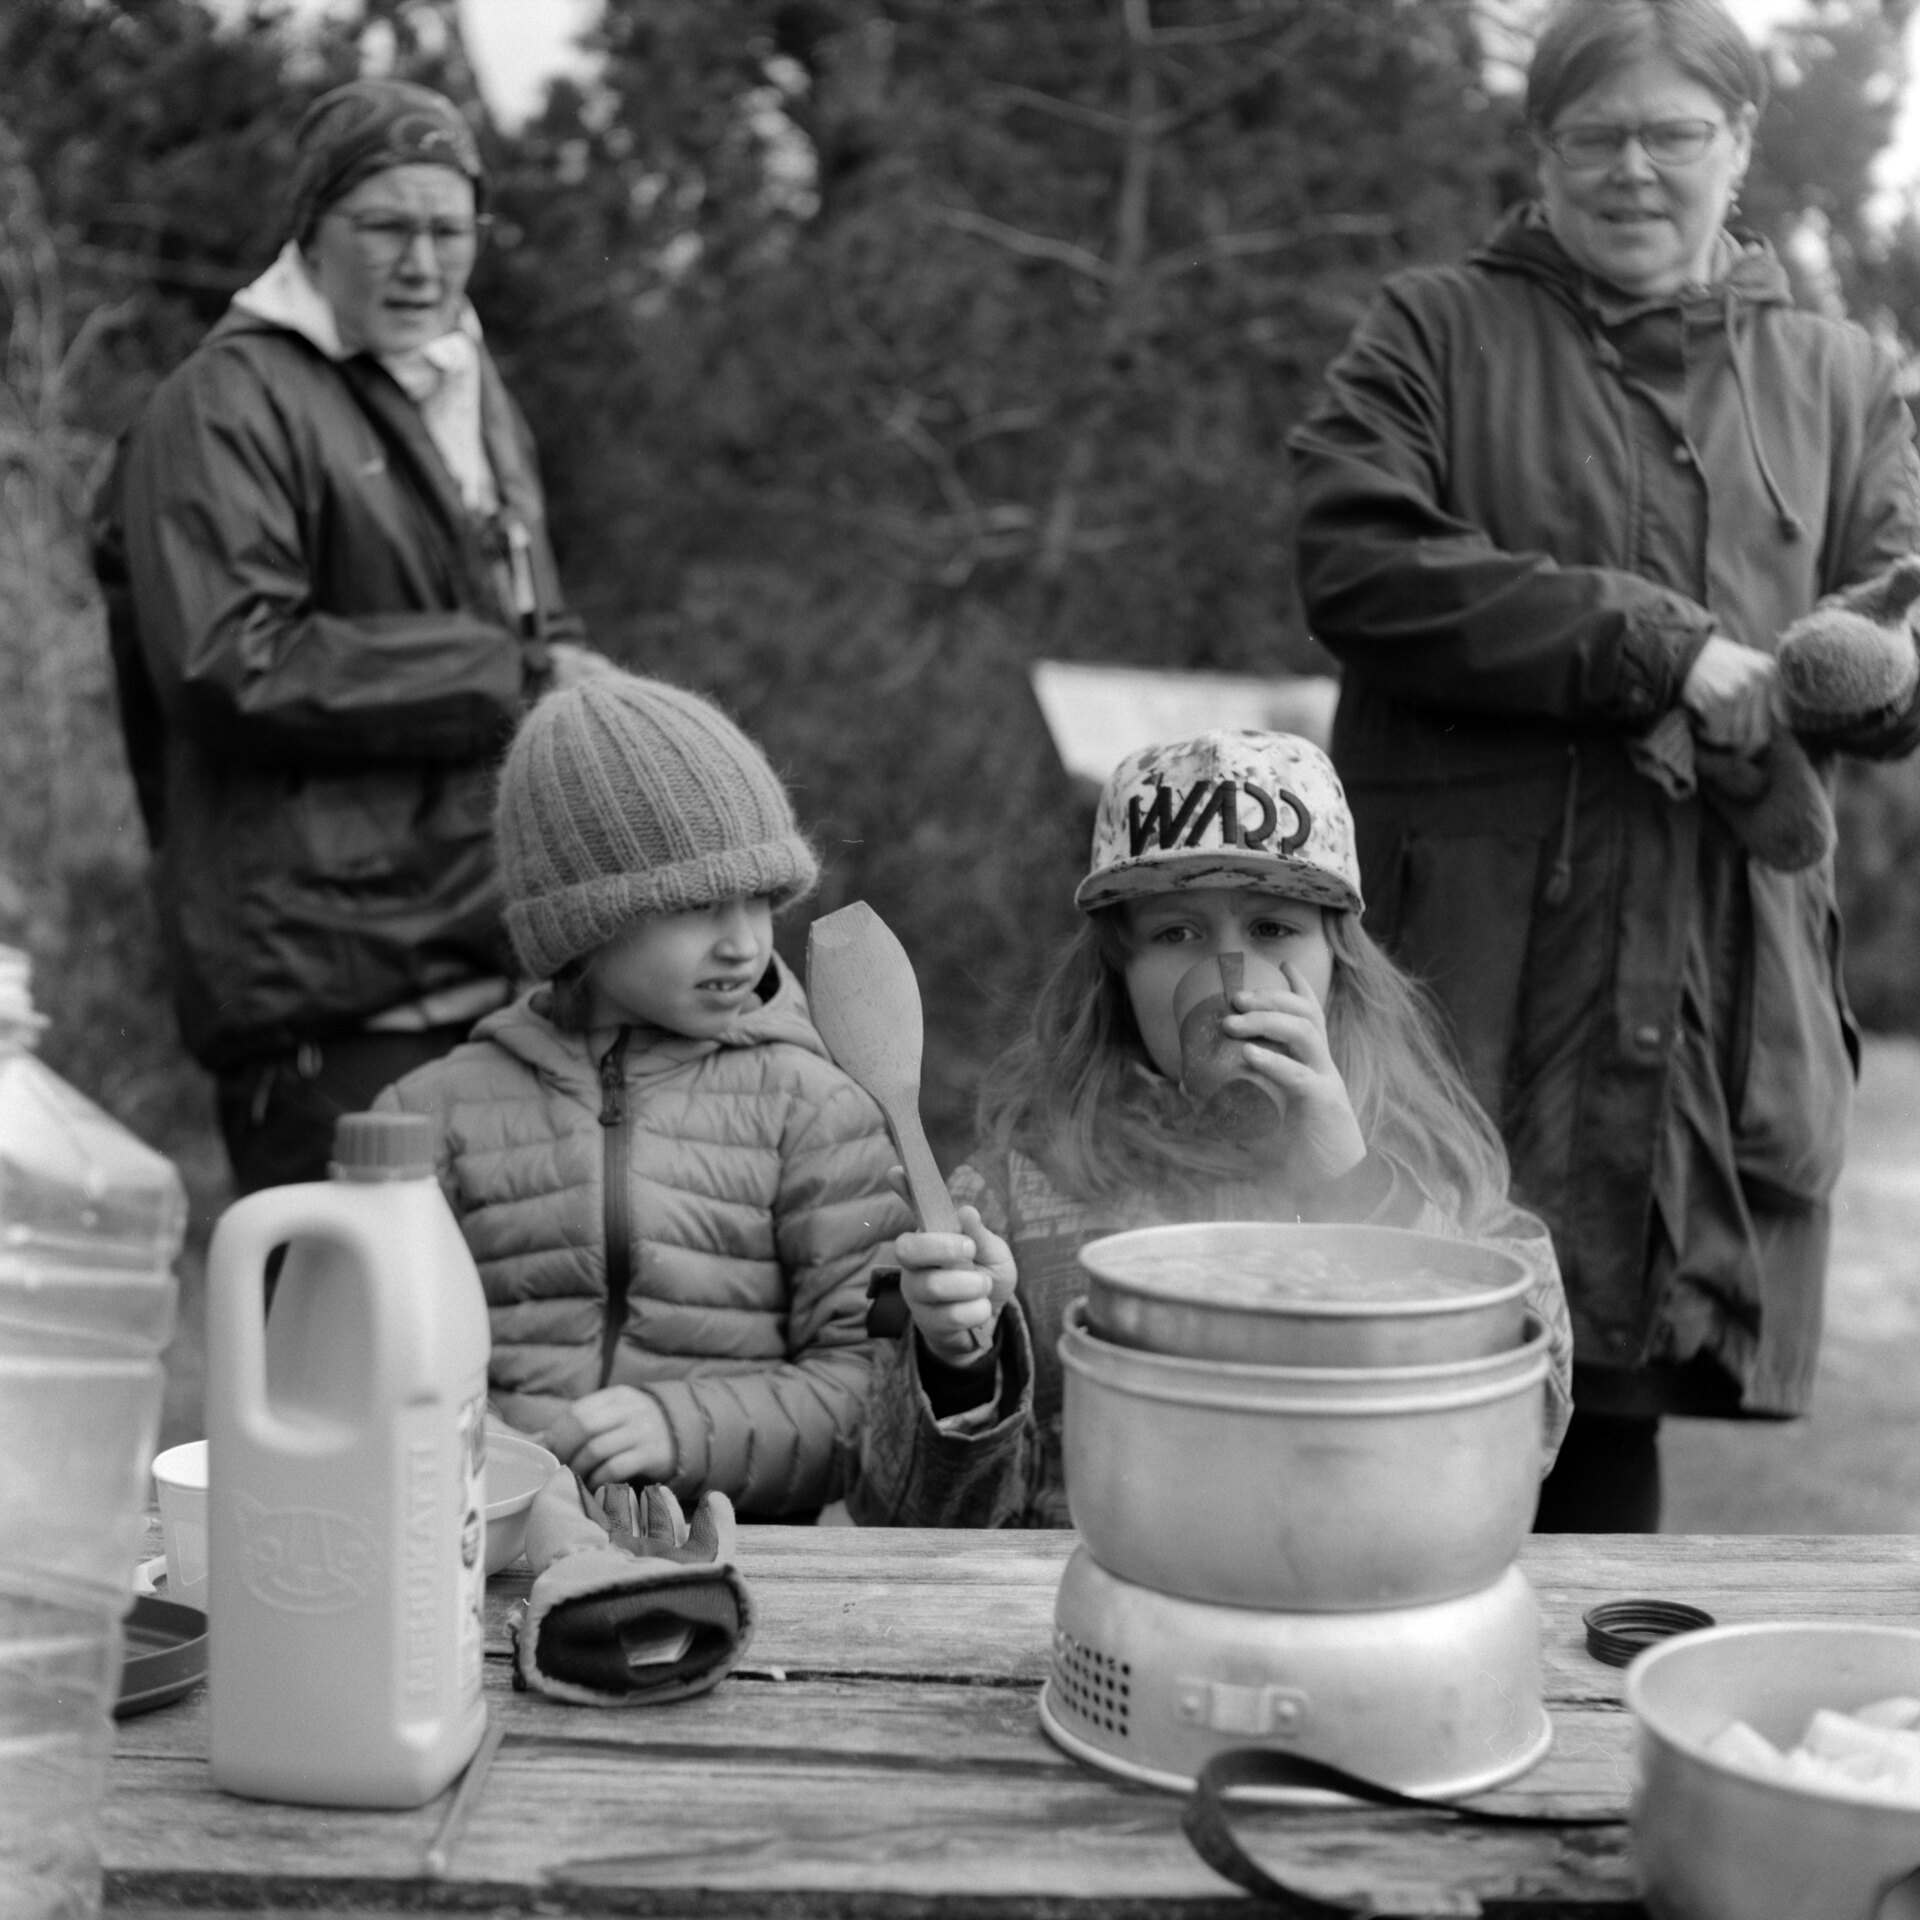
\includegraphics[width=0.8\linewidth]{assets/kolkkienpäiväretkibw14}
	\end{center}

	Retkikokki-jälkeen sisältyi luonnollisesti myös tiskaus. Kukin
	retkeläinen tiskasi omat astiansa ja trangiat, minkä jälkeen tehtiin
	ilmaisuharjoituksia Leon johdolla. Partiolaiset eivät jätä jälkeensä
	jälkiä, mikä toteutui retkellä lähes erinomaisesti. Ainoastaan yksi
	trangian polttimon kierrekorkki jäi jälkeen etsinnöistä huolimatta.

	% \columnbreak

	Johannes lähti isänsä kanssa valmistautumaan illan teatterinäytökseen
	ja muut siirtyivät retken rastitehtäviin. Rasteilla retkeläiset
	pääsivät oppimaan uusia kasvien ja jäkälien nimiä
	Jumbobonus-hippaleikissä, ilmaisemaan luovuuttaan ja kekseliäisyyttään
	tekemällä miniatyyri-installaation, verestämään muistiaan lintulajien
	muistipelissä sekä löytämään sisäisen valokuvaajansa ottamalla hauskoja
	valokuvia – joita voit nähdä seuravalla sivulla!

	% \vspace*{0.16cm}

	\vspace*{0.16cm}
	\begin{center}
		\noindent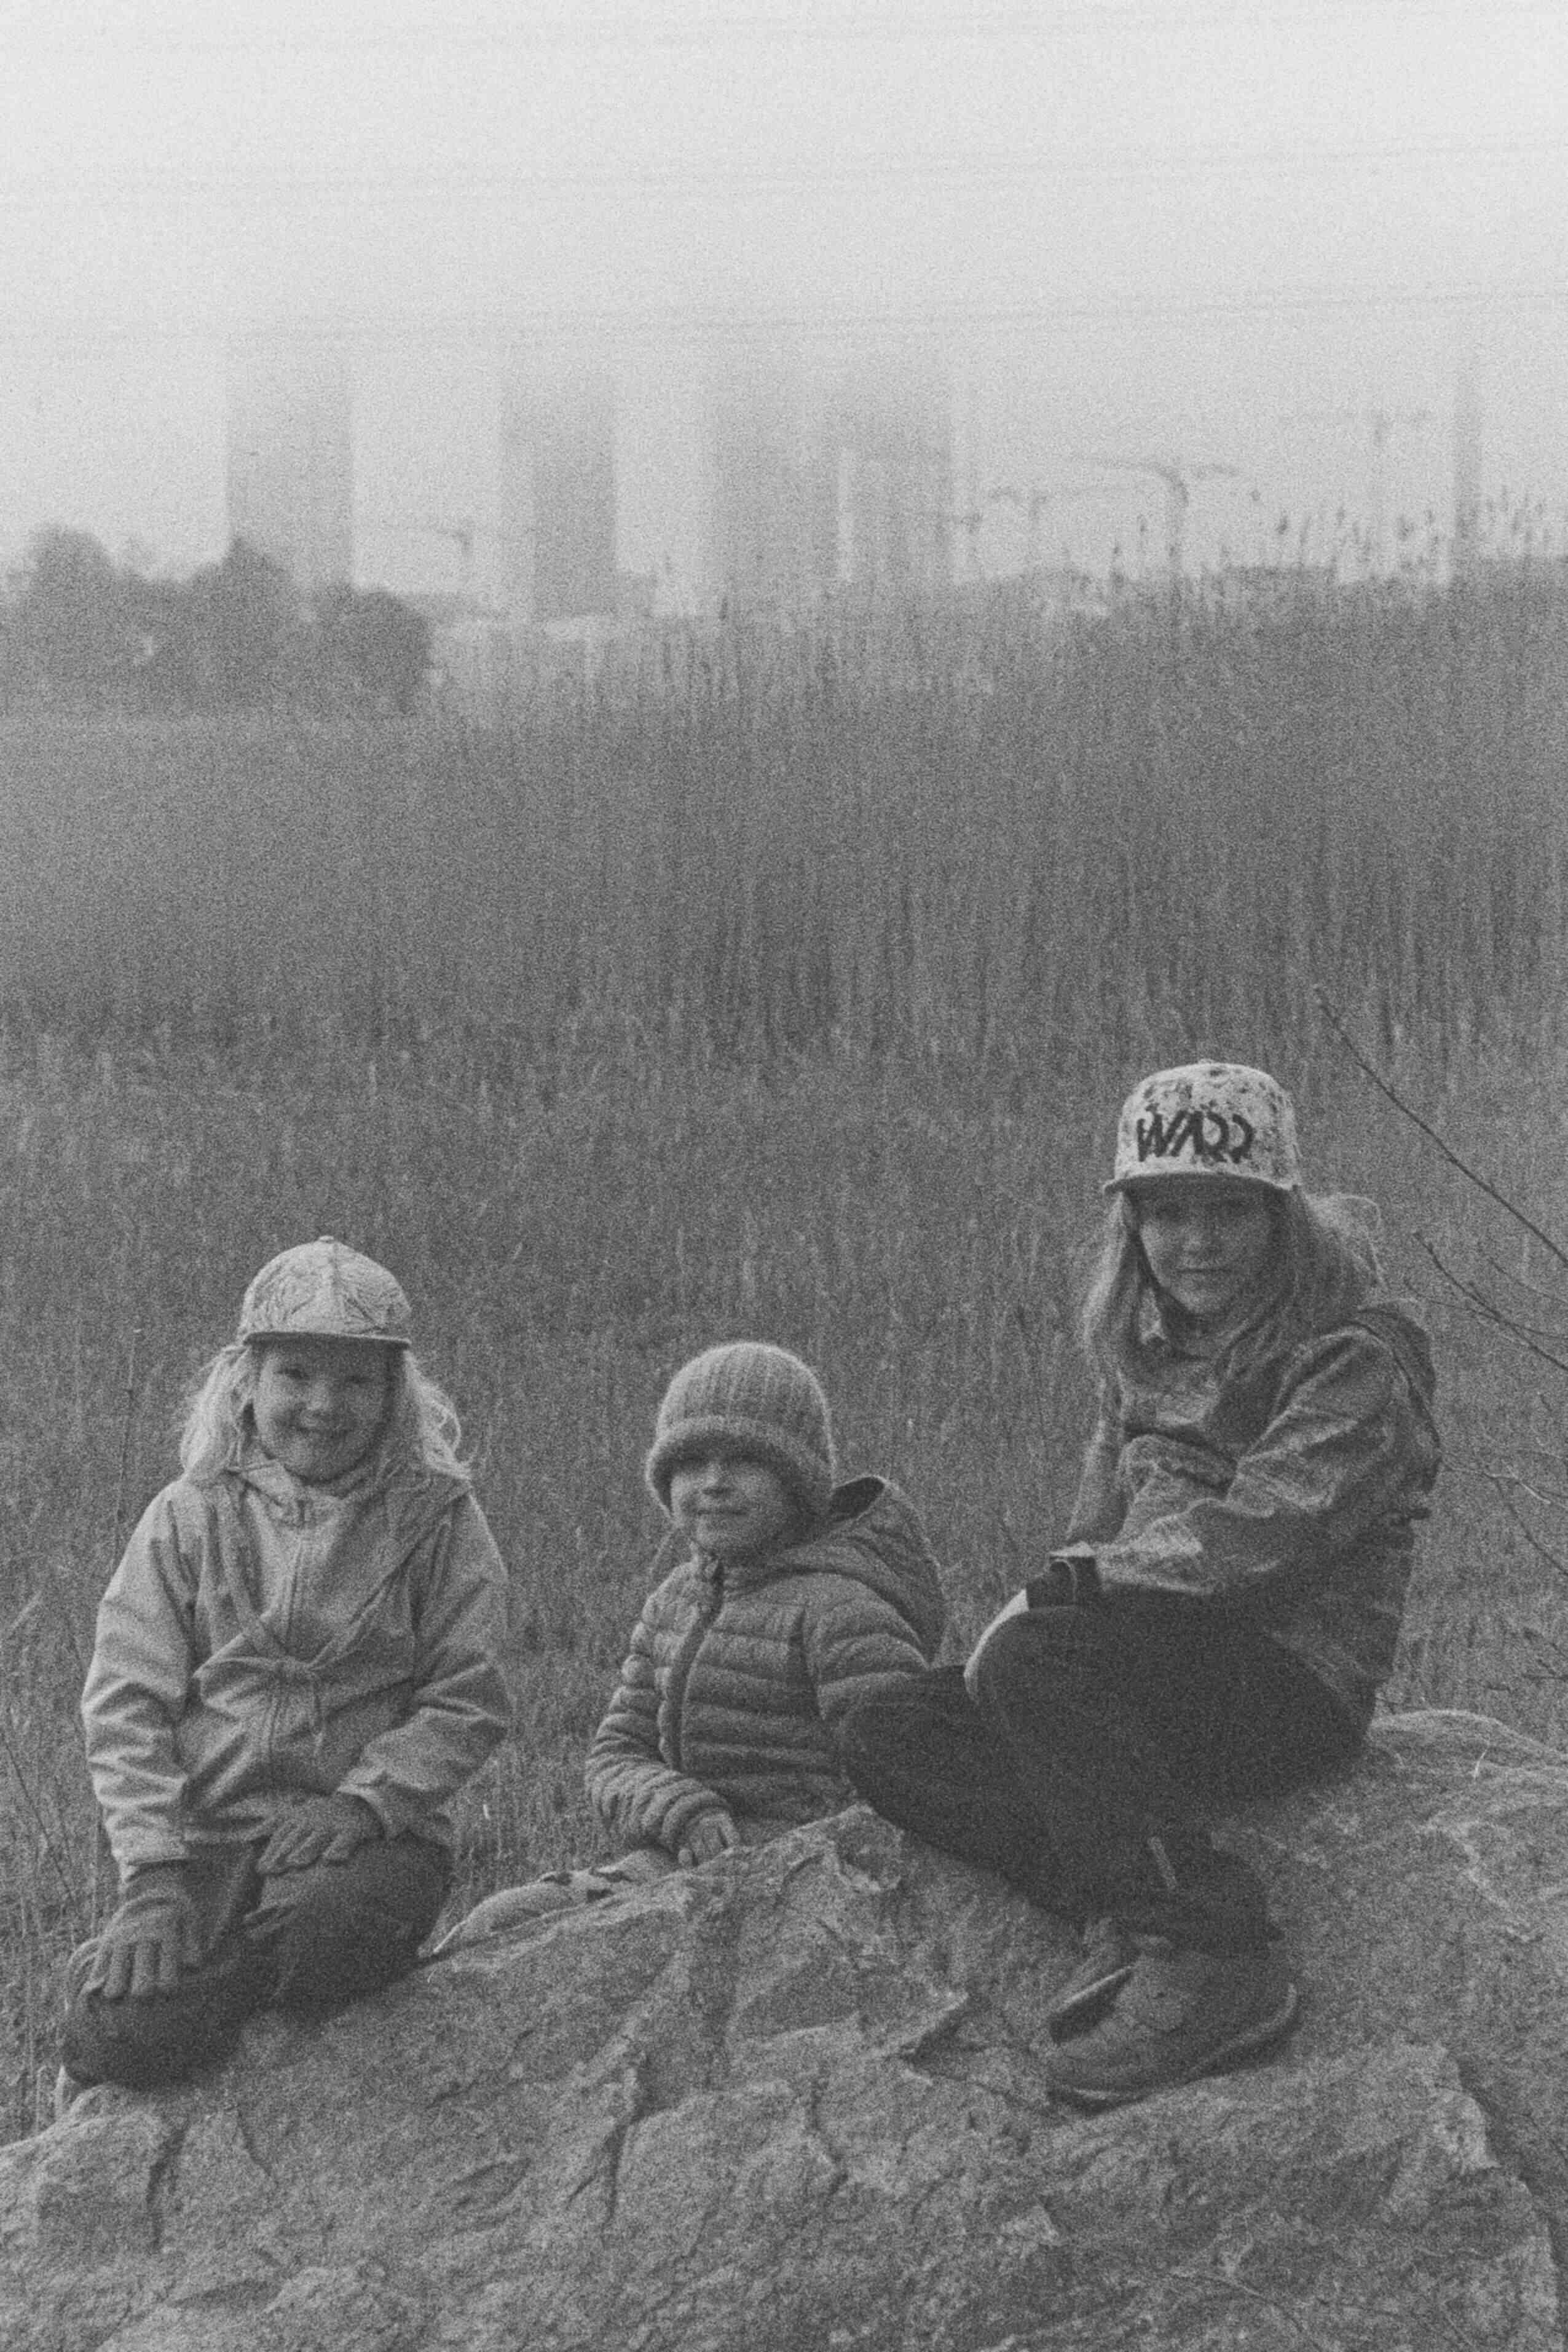
\includegraphics[width=0.8\linewidth]{assets/kolkkienpäiväretkibw13}
	\end{center}

	% \columnbreak

	Aikaa ei enää ollut lähteä kiertämään Viikin muita lintutorneja, vaan
	rastien jälkeen pidettiin lyhyt evästauko ja päätettiin suunnata
	takaisin kohti Viikin tiedepuiston bussipysäkkiä. Osa retkueesta jatkoi
	Nonnan kyydillä hänen kotiinsa Hiekkaharjuun illan johtajahuoltoa
	varten.




\end{multicols}
\vspace*{1.28cm}

\medskip
\noindent\null\hfill Kuvat: Tanguy Gérôme \& Janne Suomalainen\\
\noindent\null\hfill Teksti: Janne Suomalainen

% \vspace*{-0.64cm}

\clearpage

\textbf{Valokuvausrastin tulos:}

\begin{multicols}{2}

	\centering
	\noindent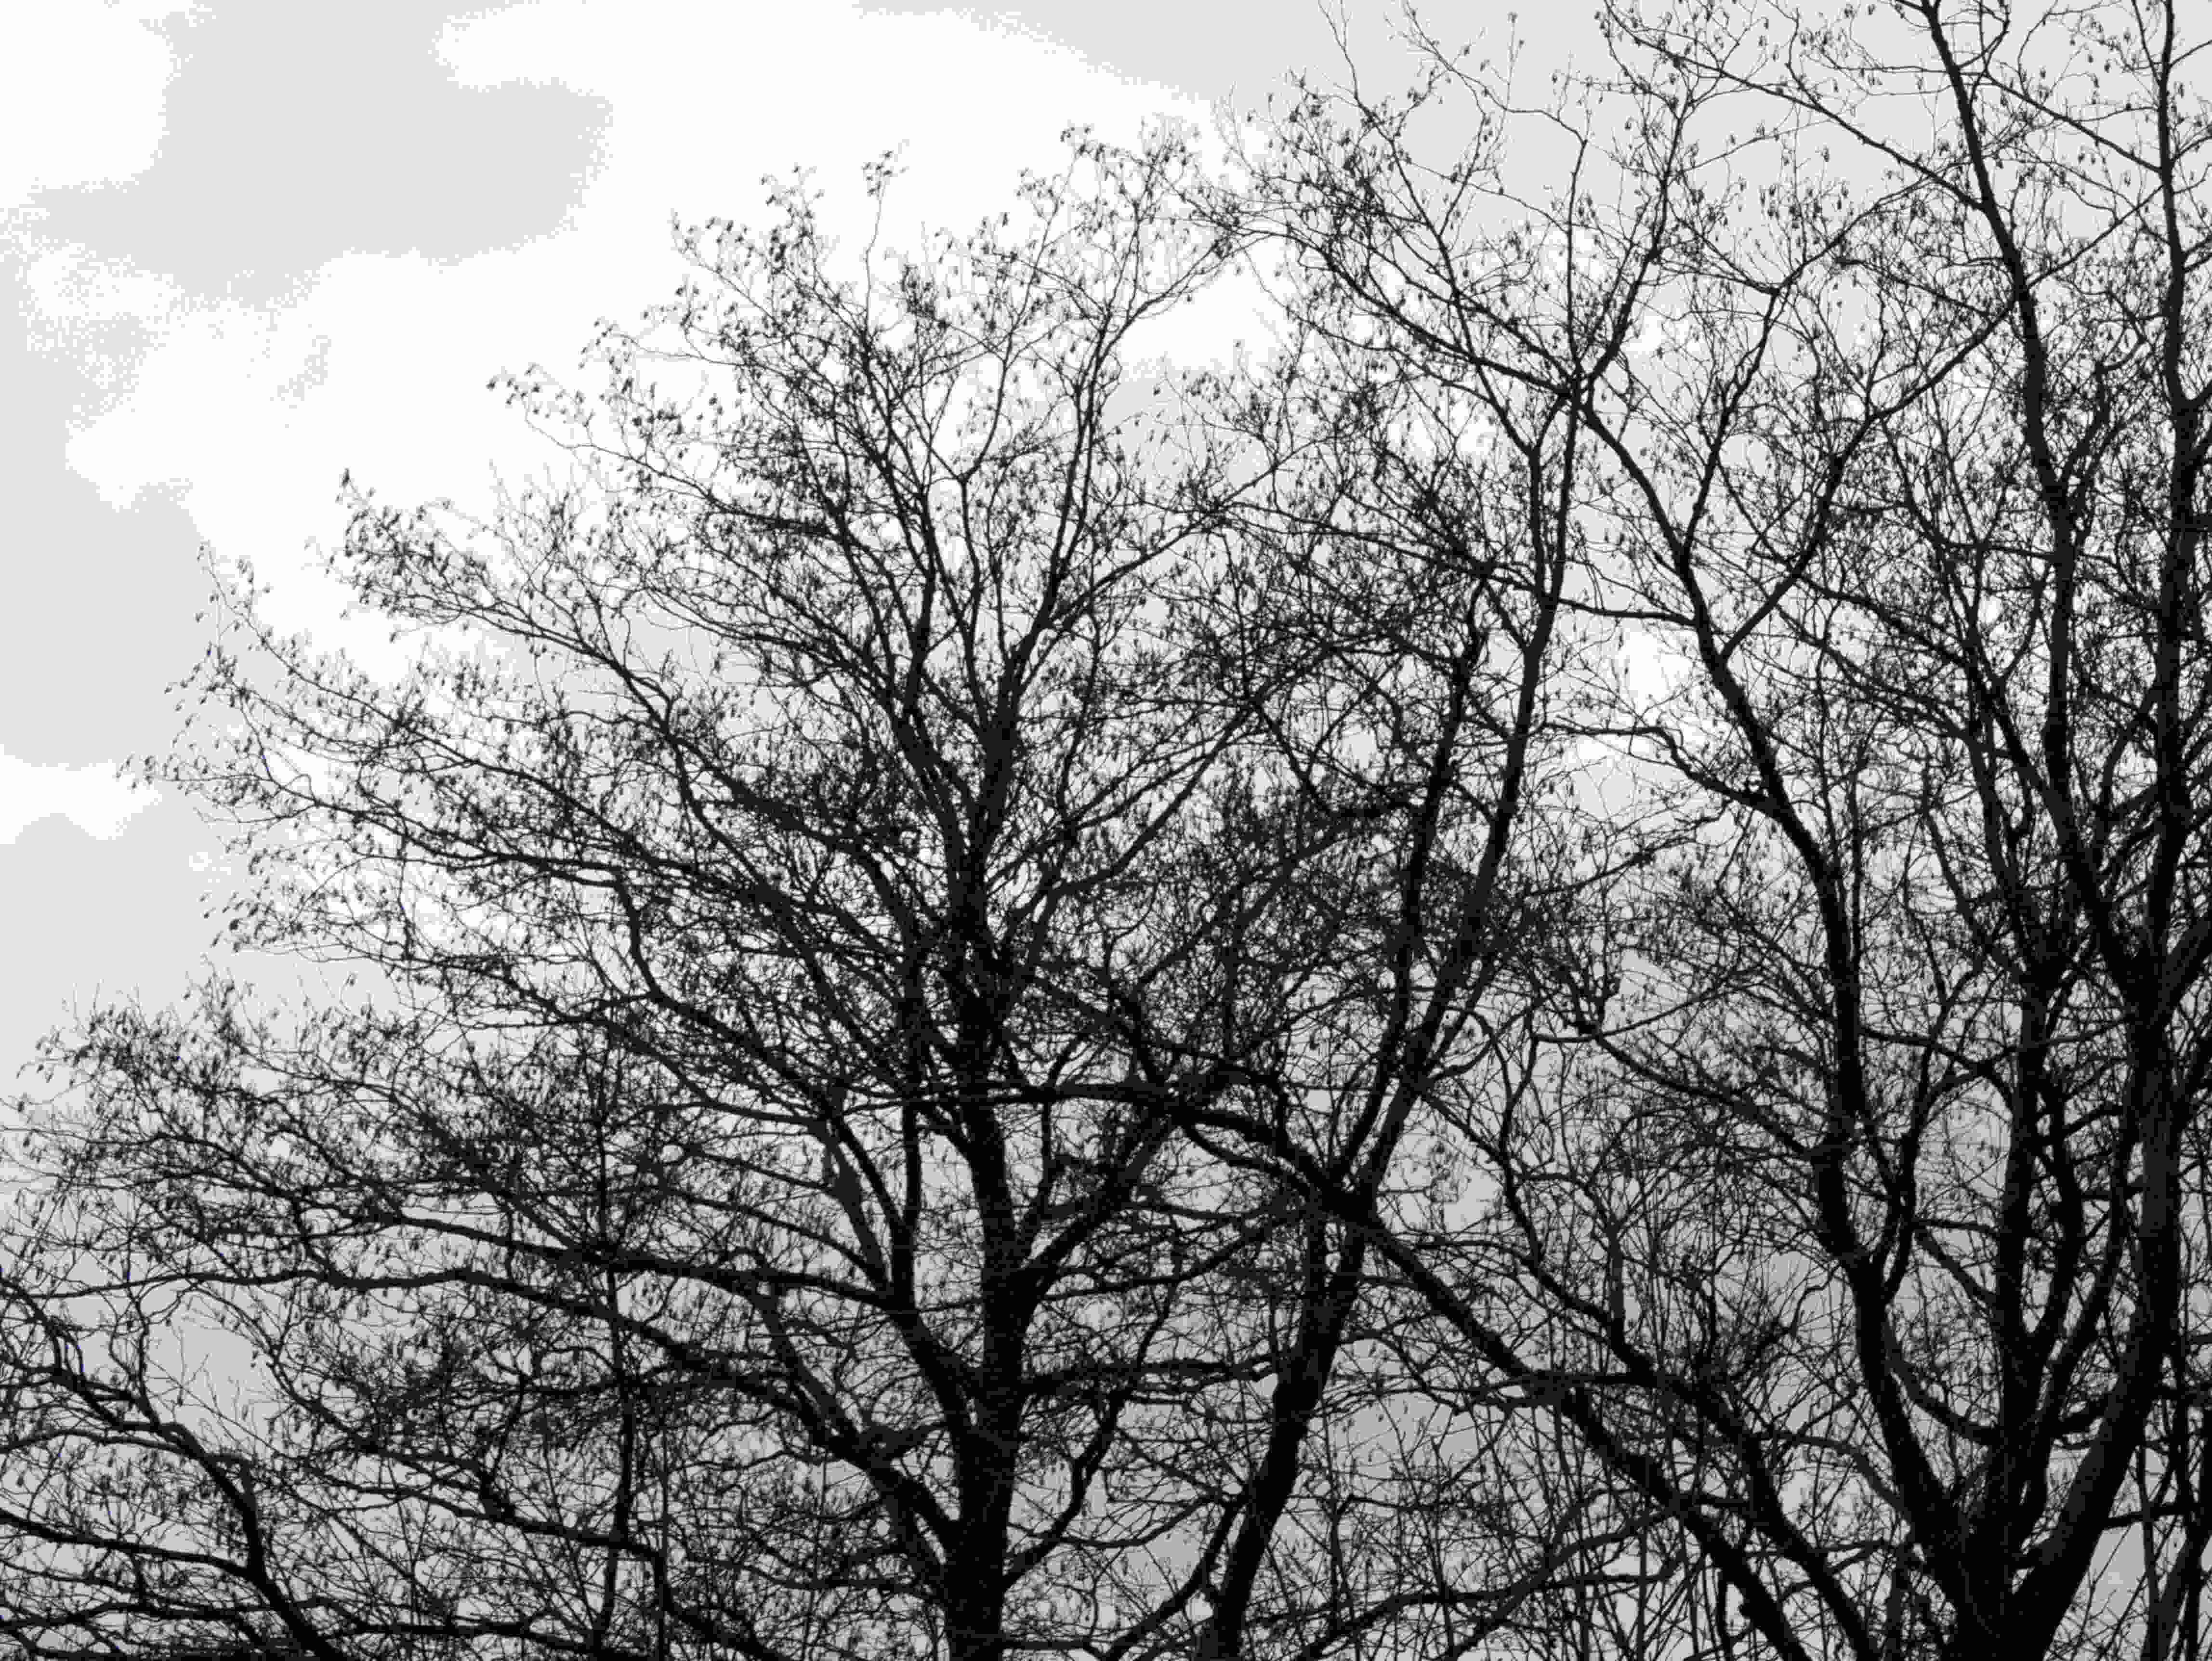
\includegraphics[width=0.9\linewidth]{assets/kolkkienpäiväretki4}
	\noindent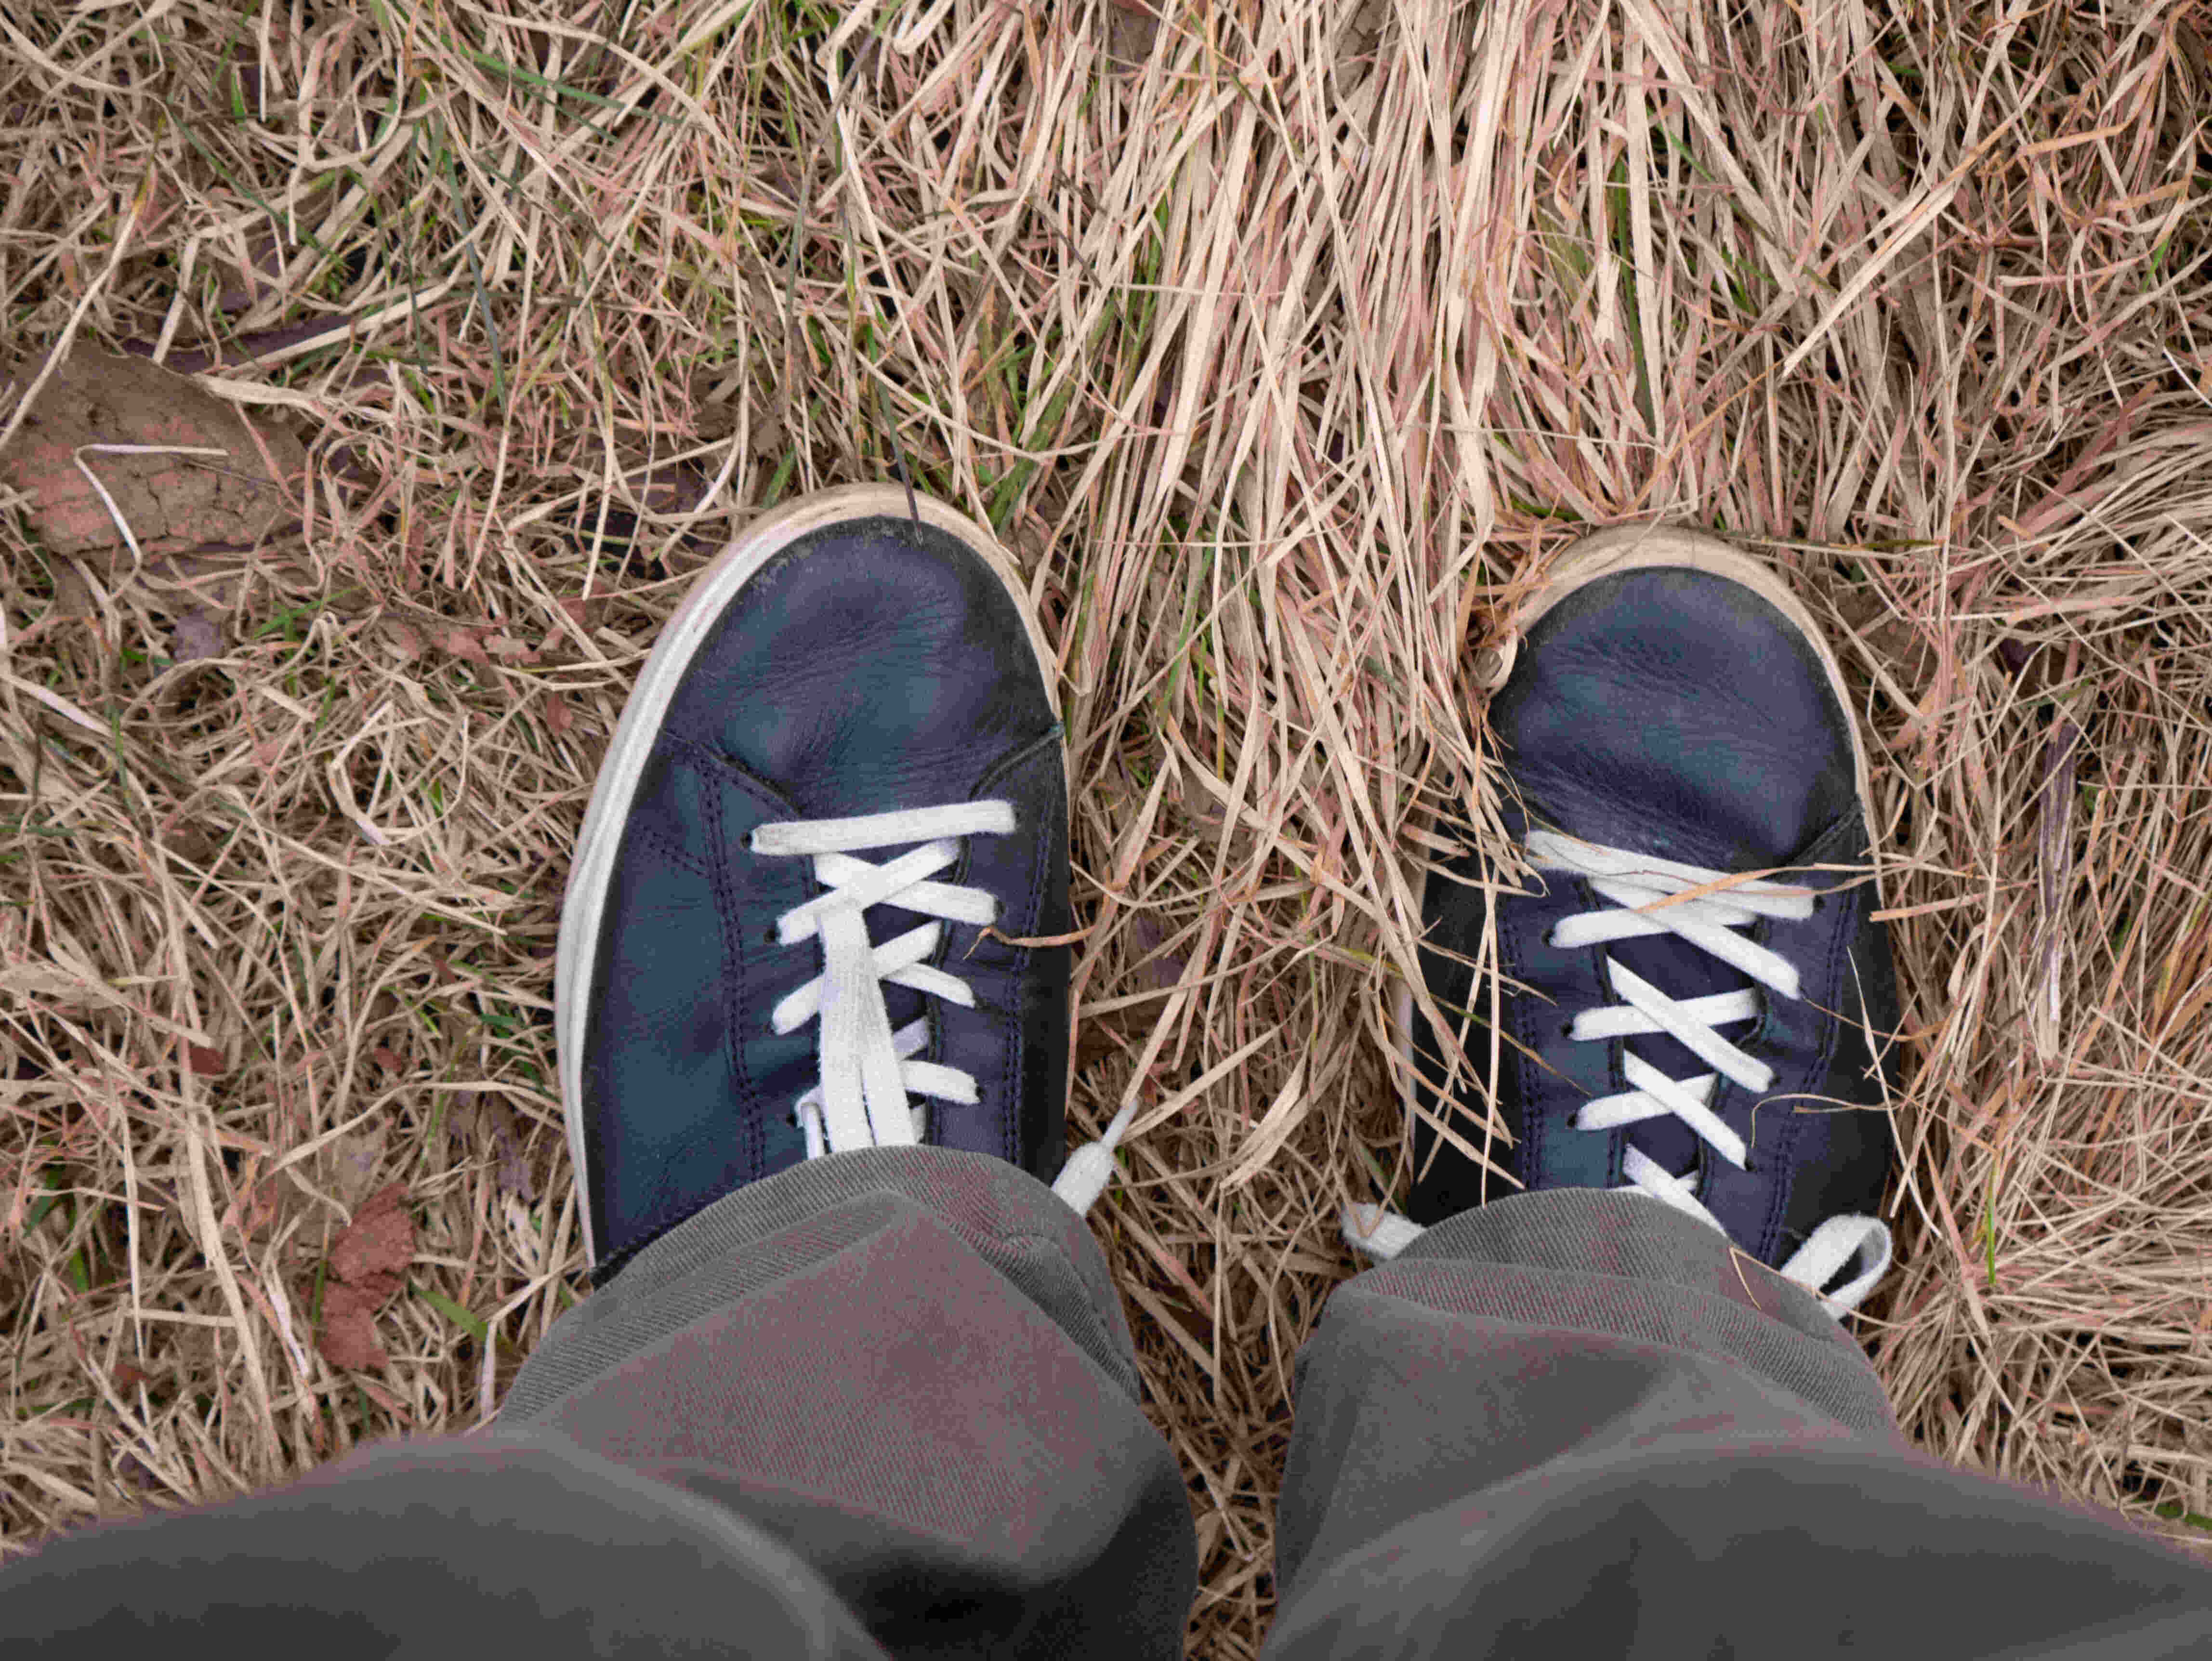
\includegraphics[width=0.9\linewidth]{assets/kolkkienpäiväretki5}
	\noindent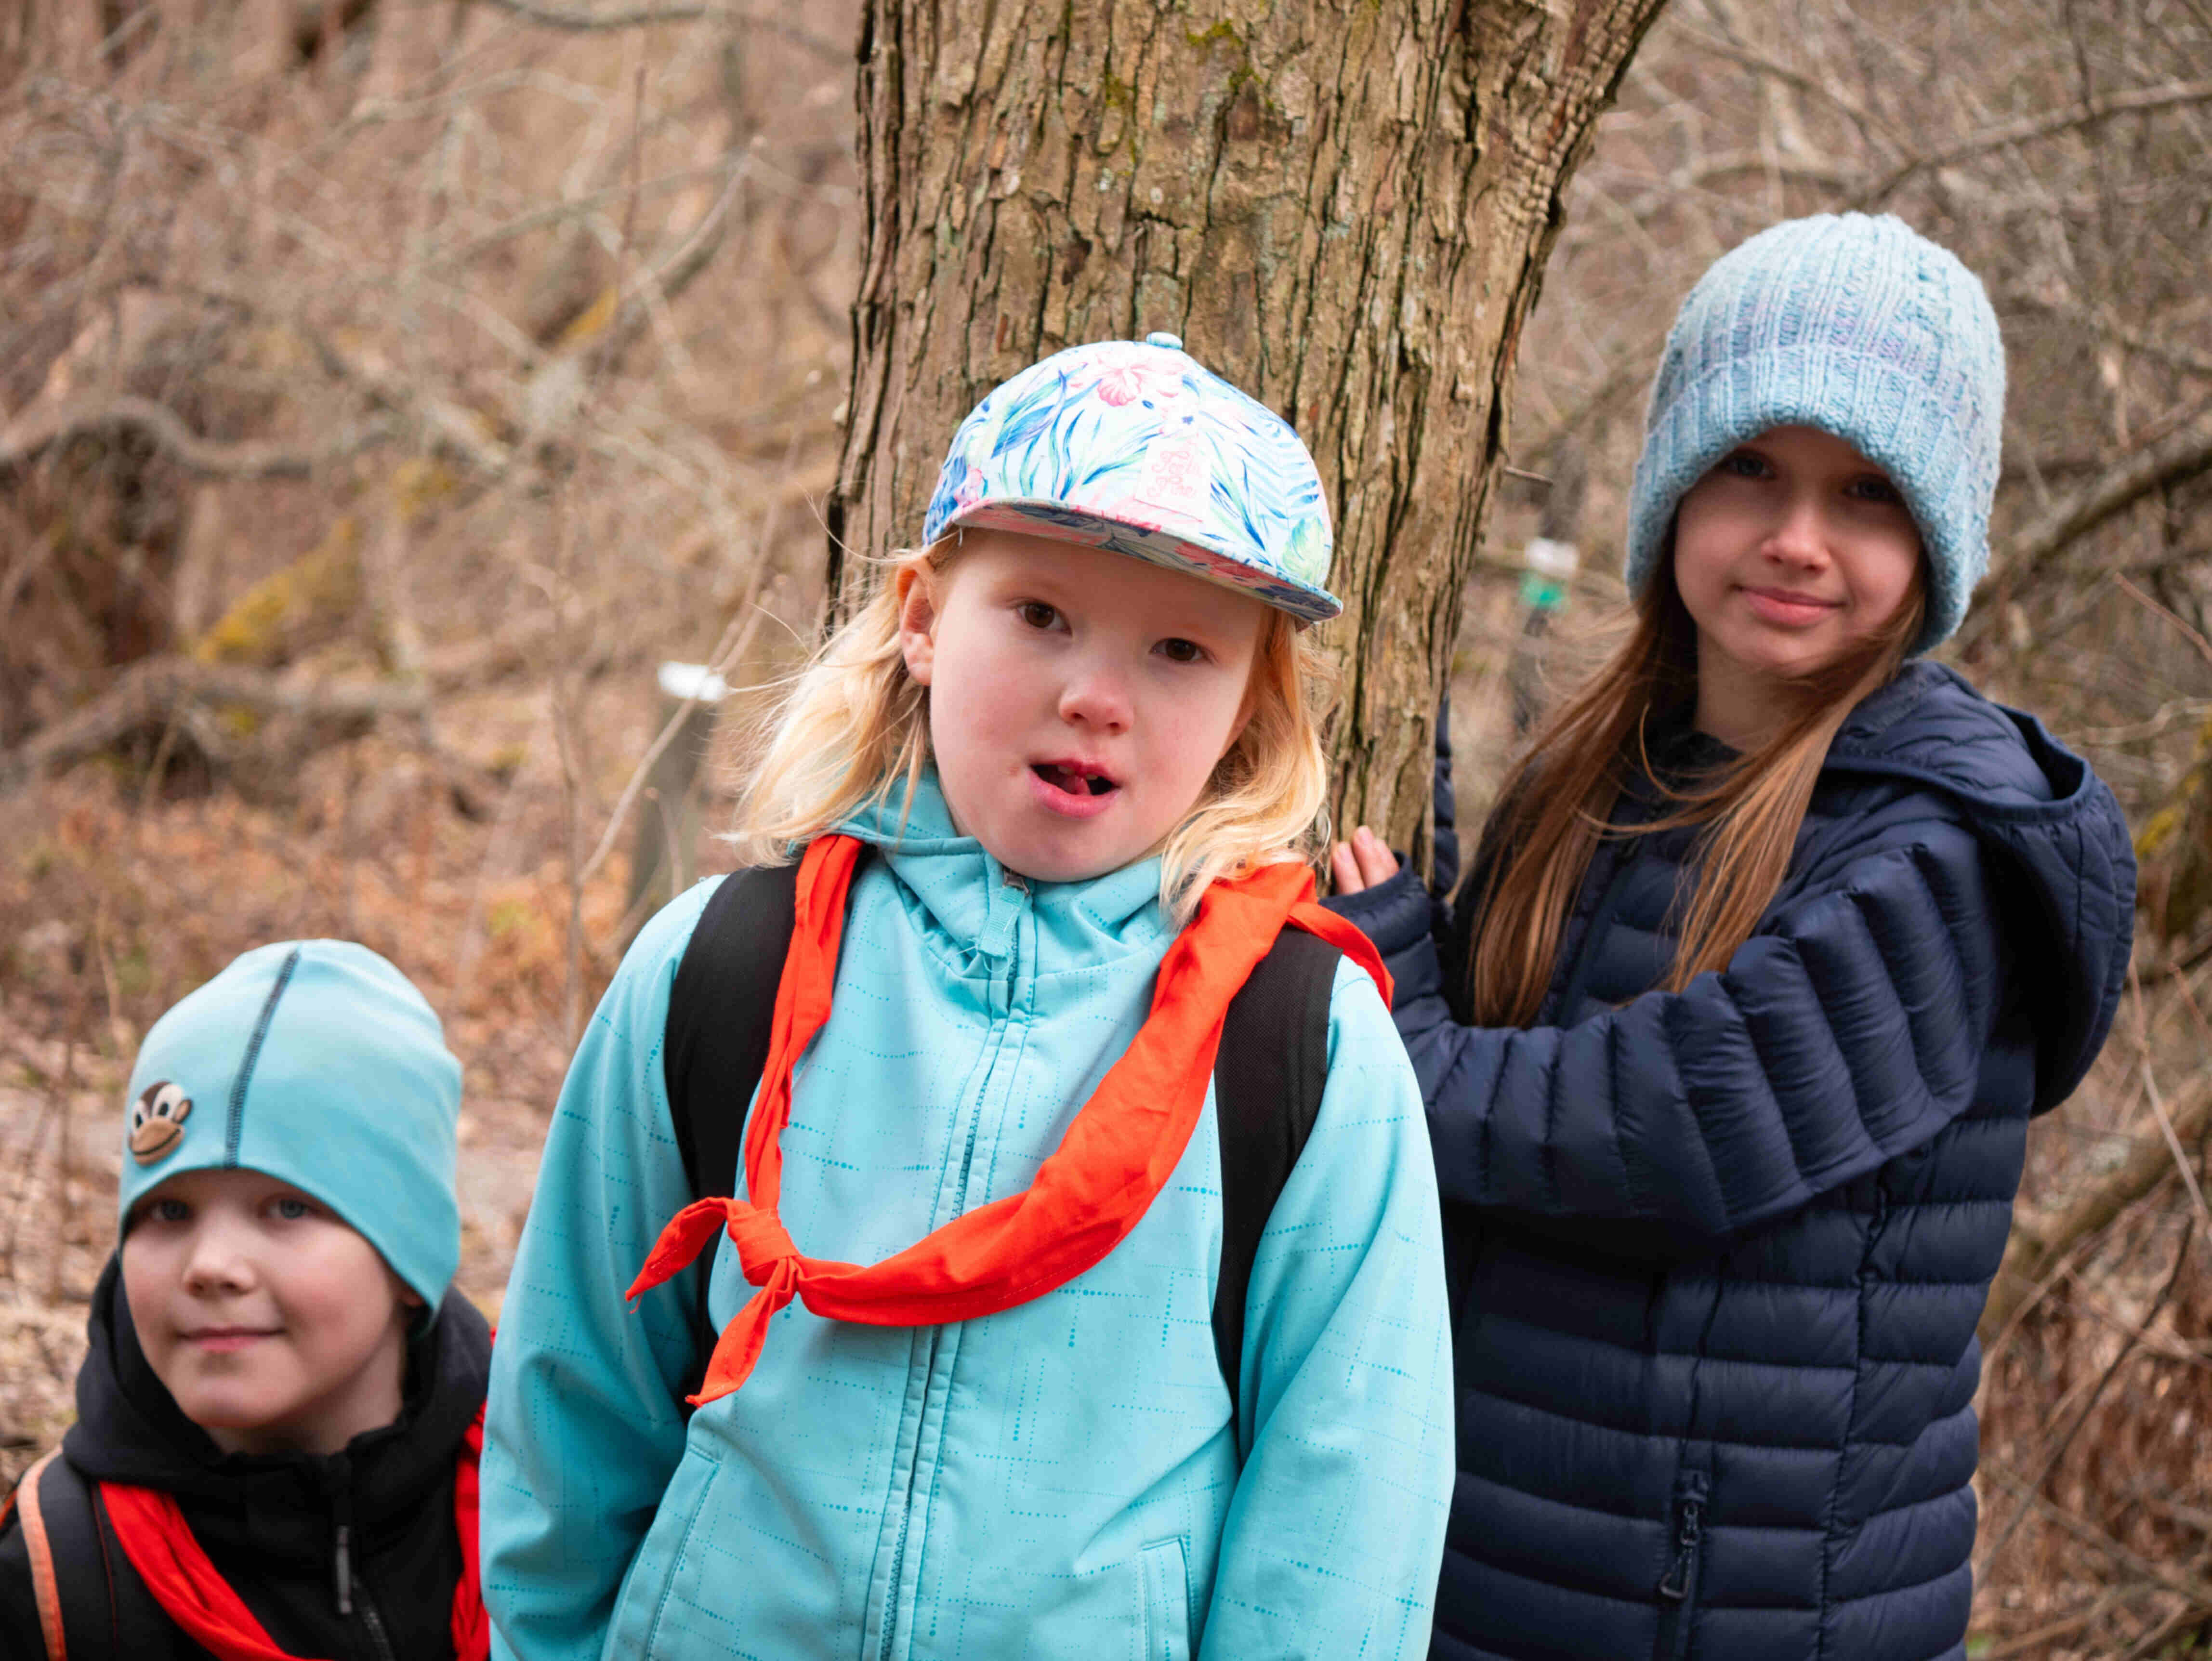
\includegraphics[width=0.9\linewidth]{assets/kolkkienpäiväretki6}
	\noindent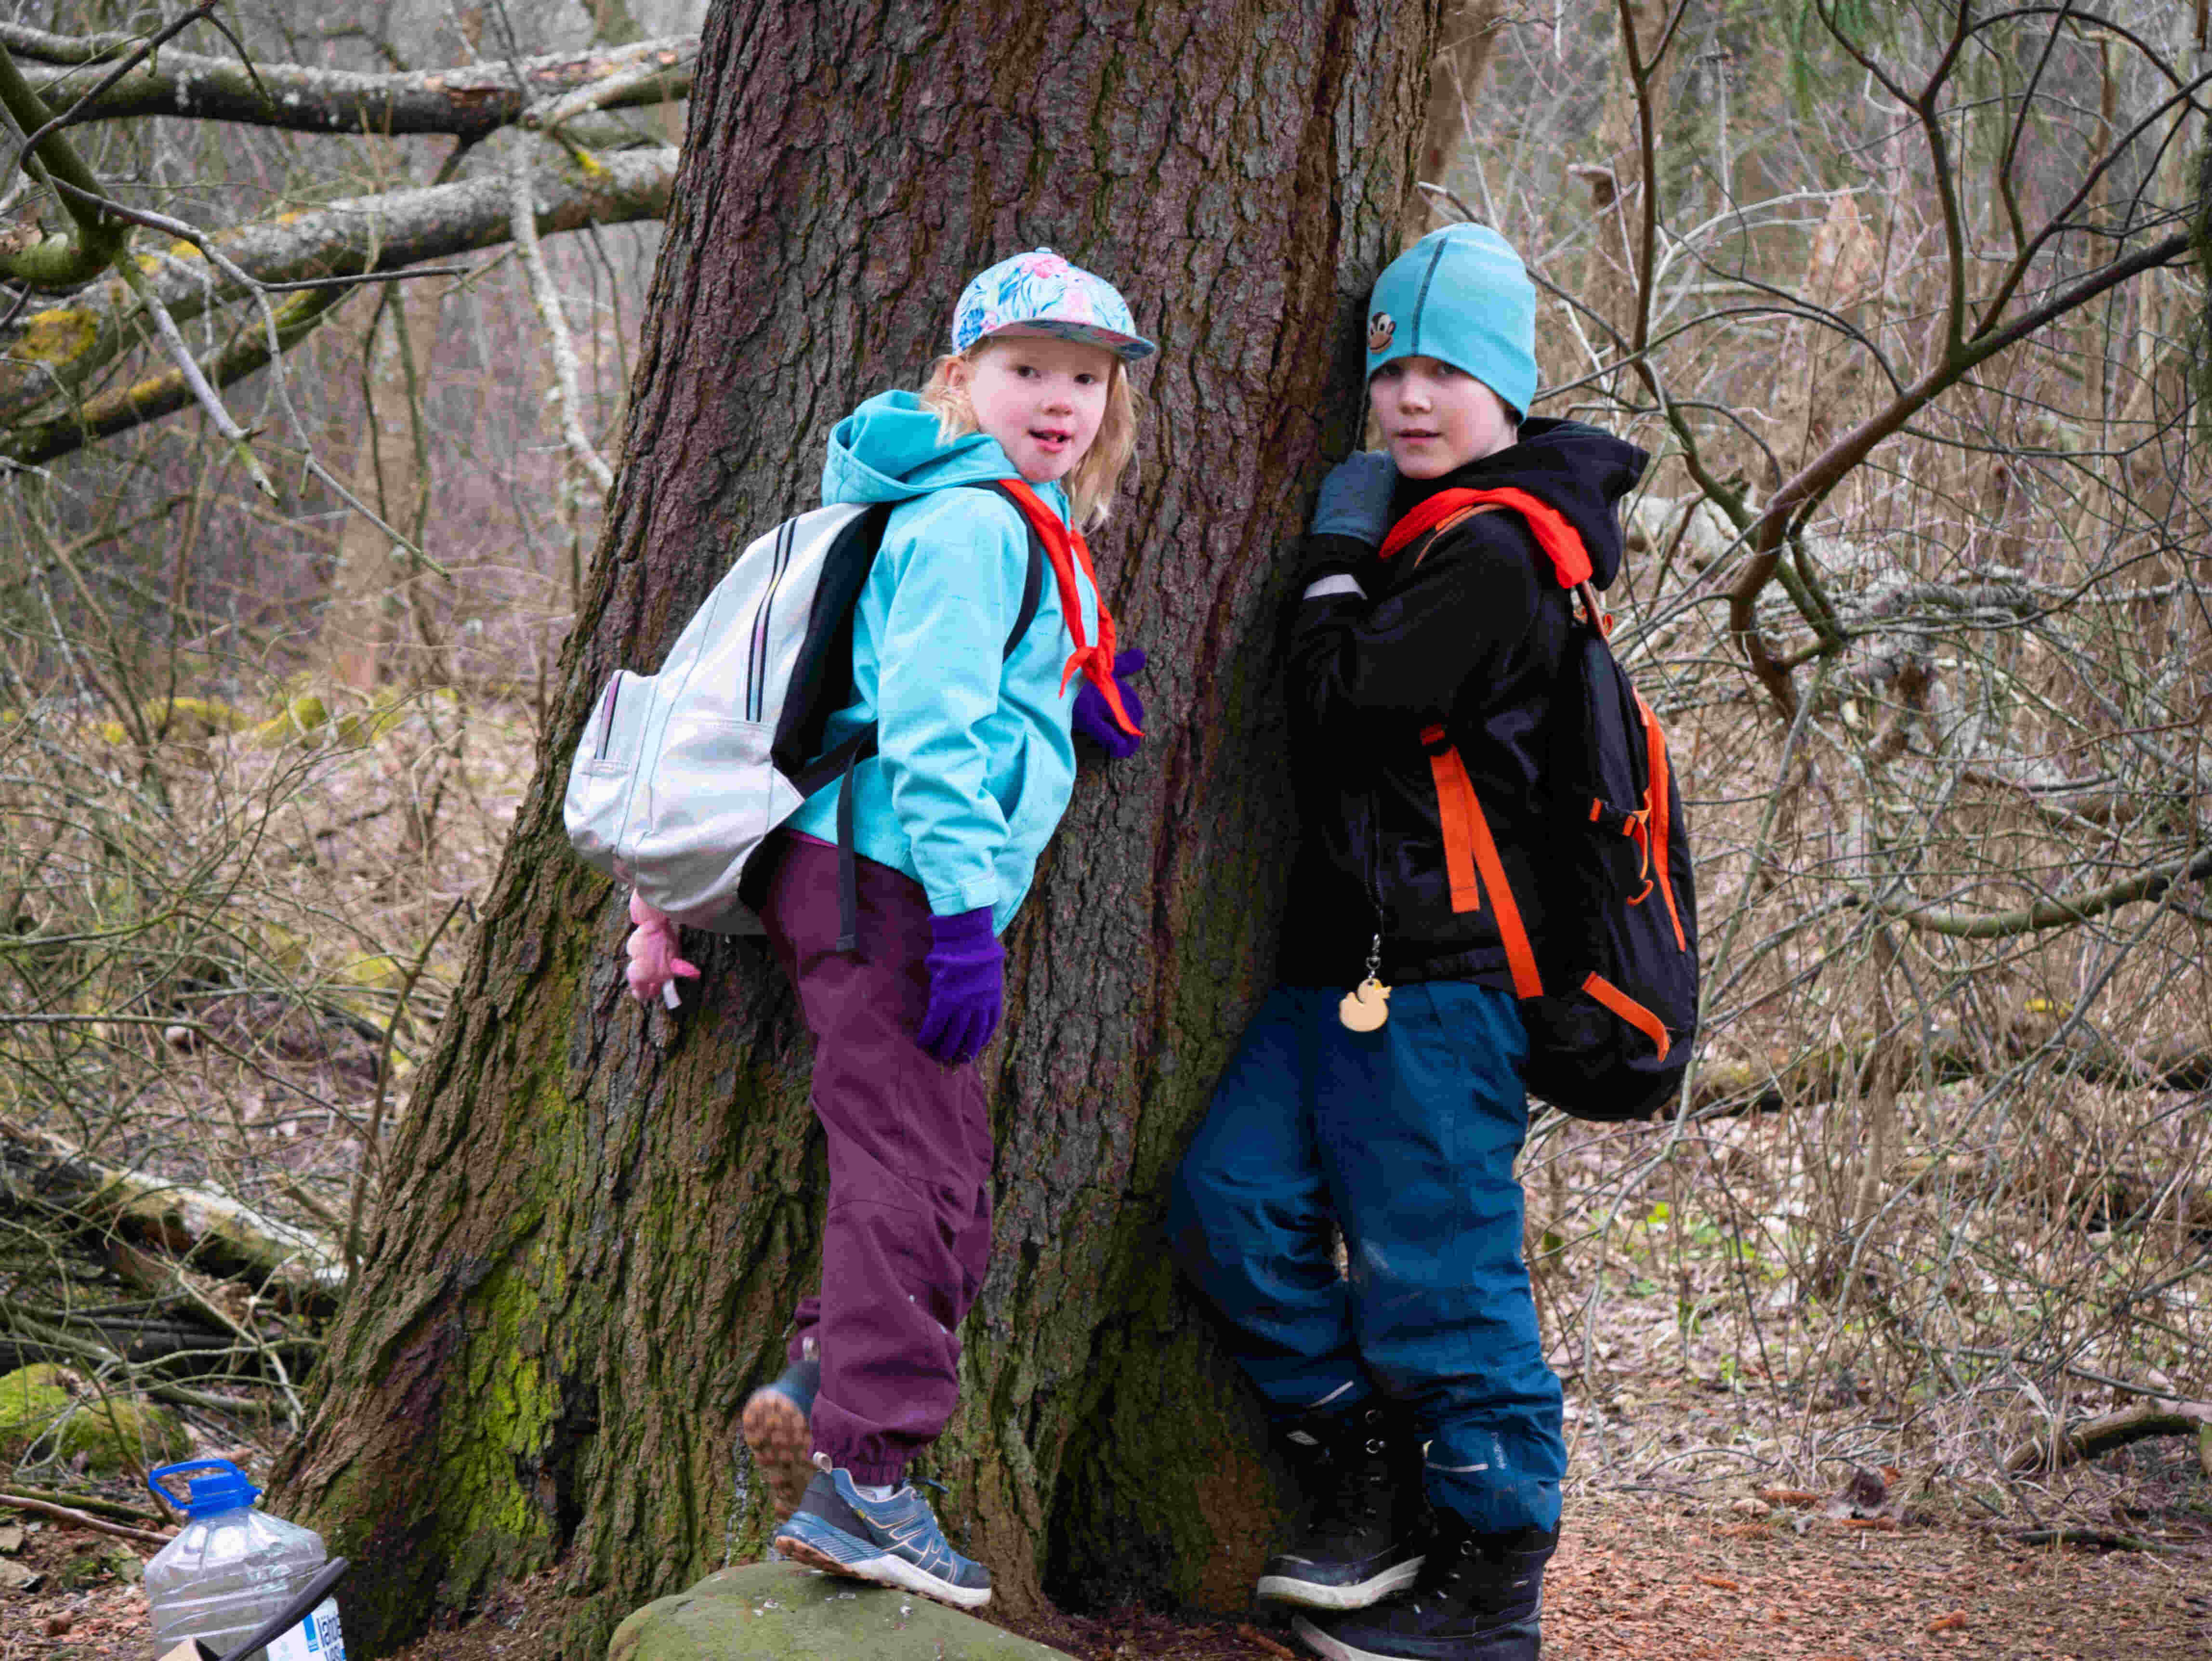
\includegraphics[width=0.9\linewidth]{assets/kolkkienpäiväretki7}
	% \noindent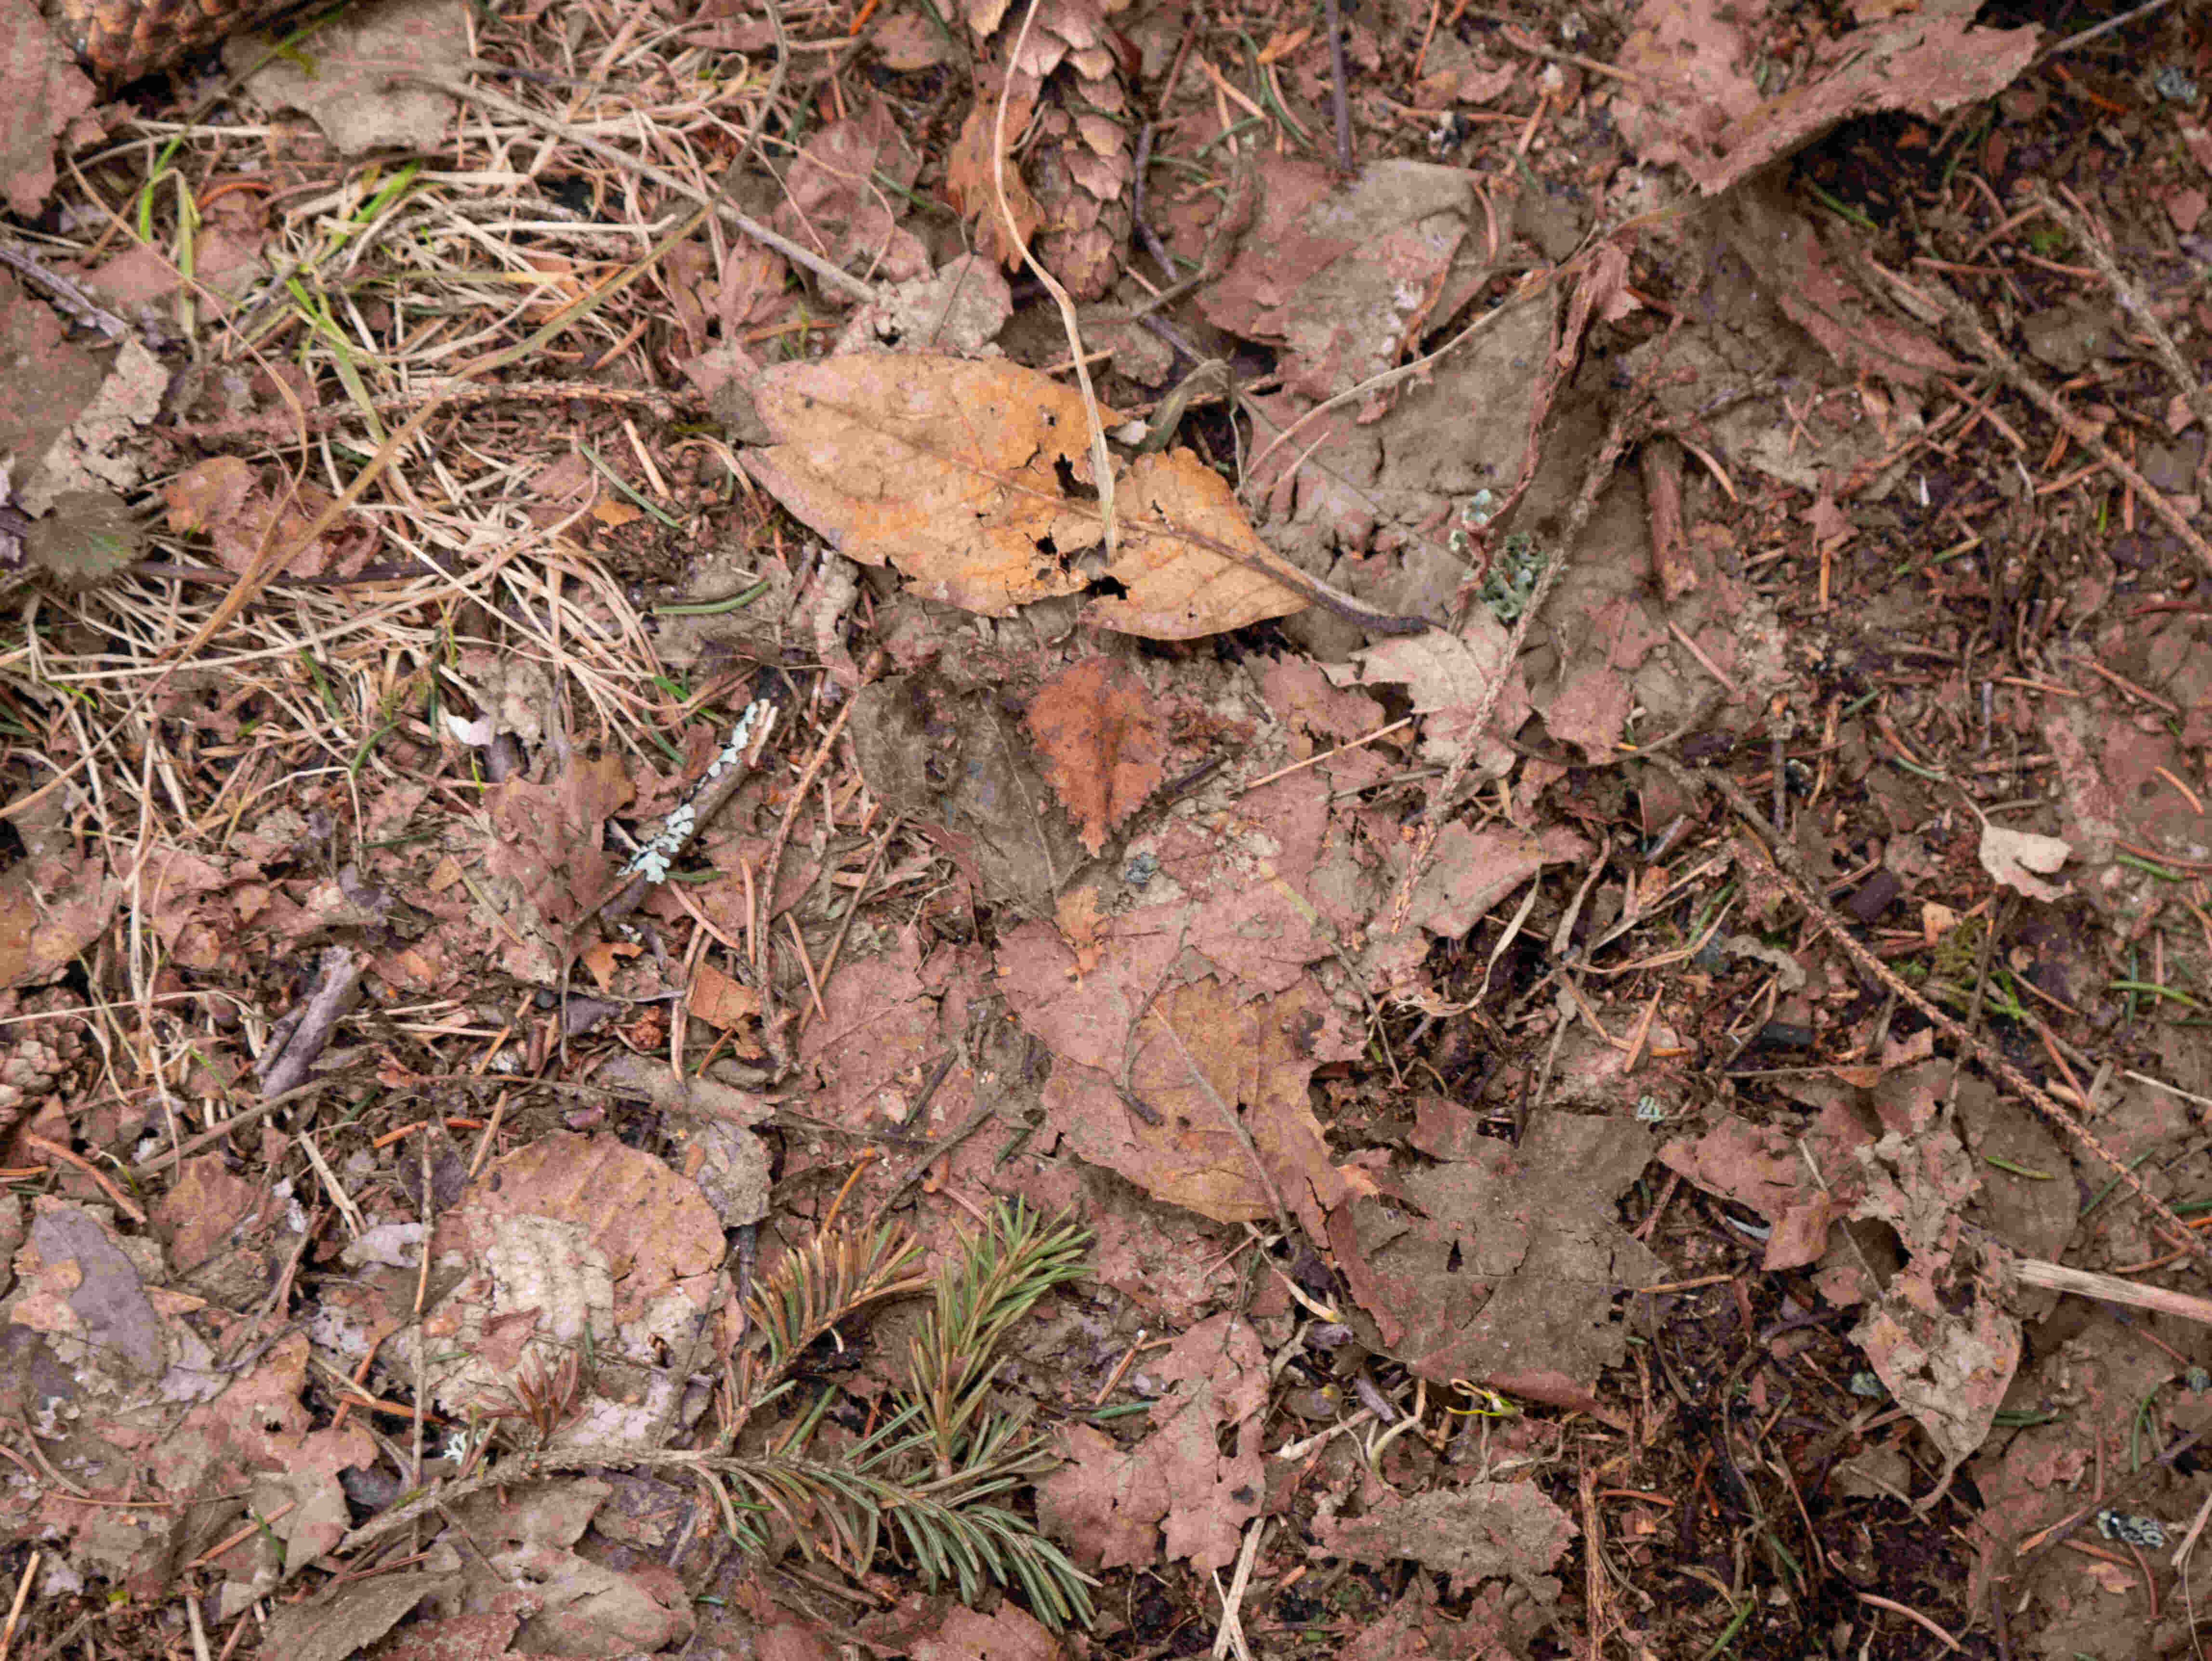
\includegraphics[width=0.9\linewidth]{assets/kolkkienpäiväretki8}
	\noindent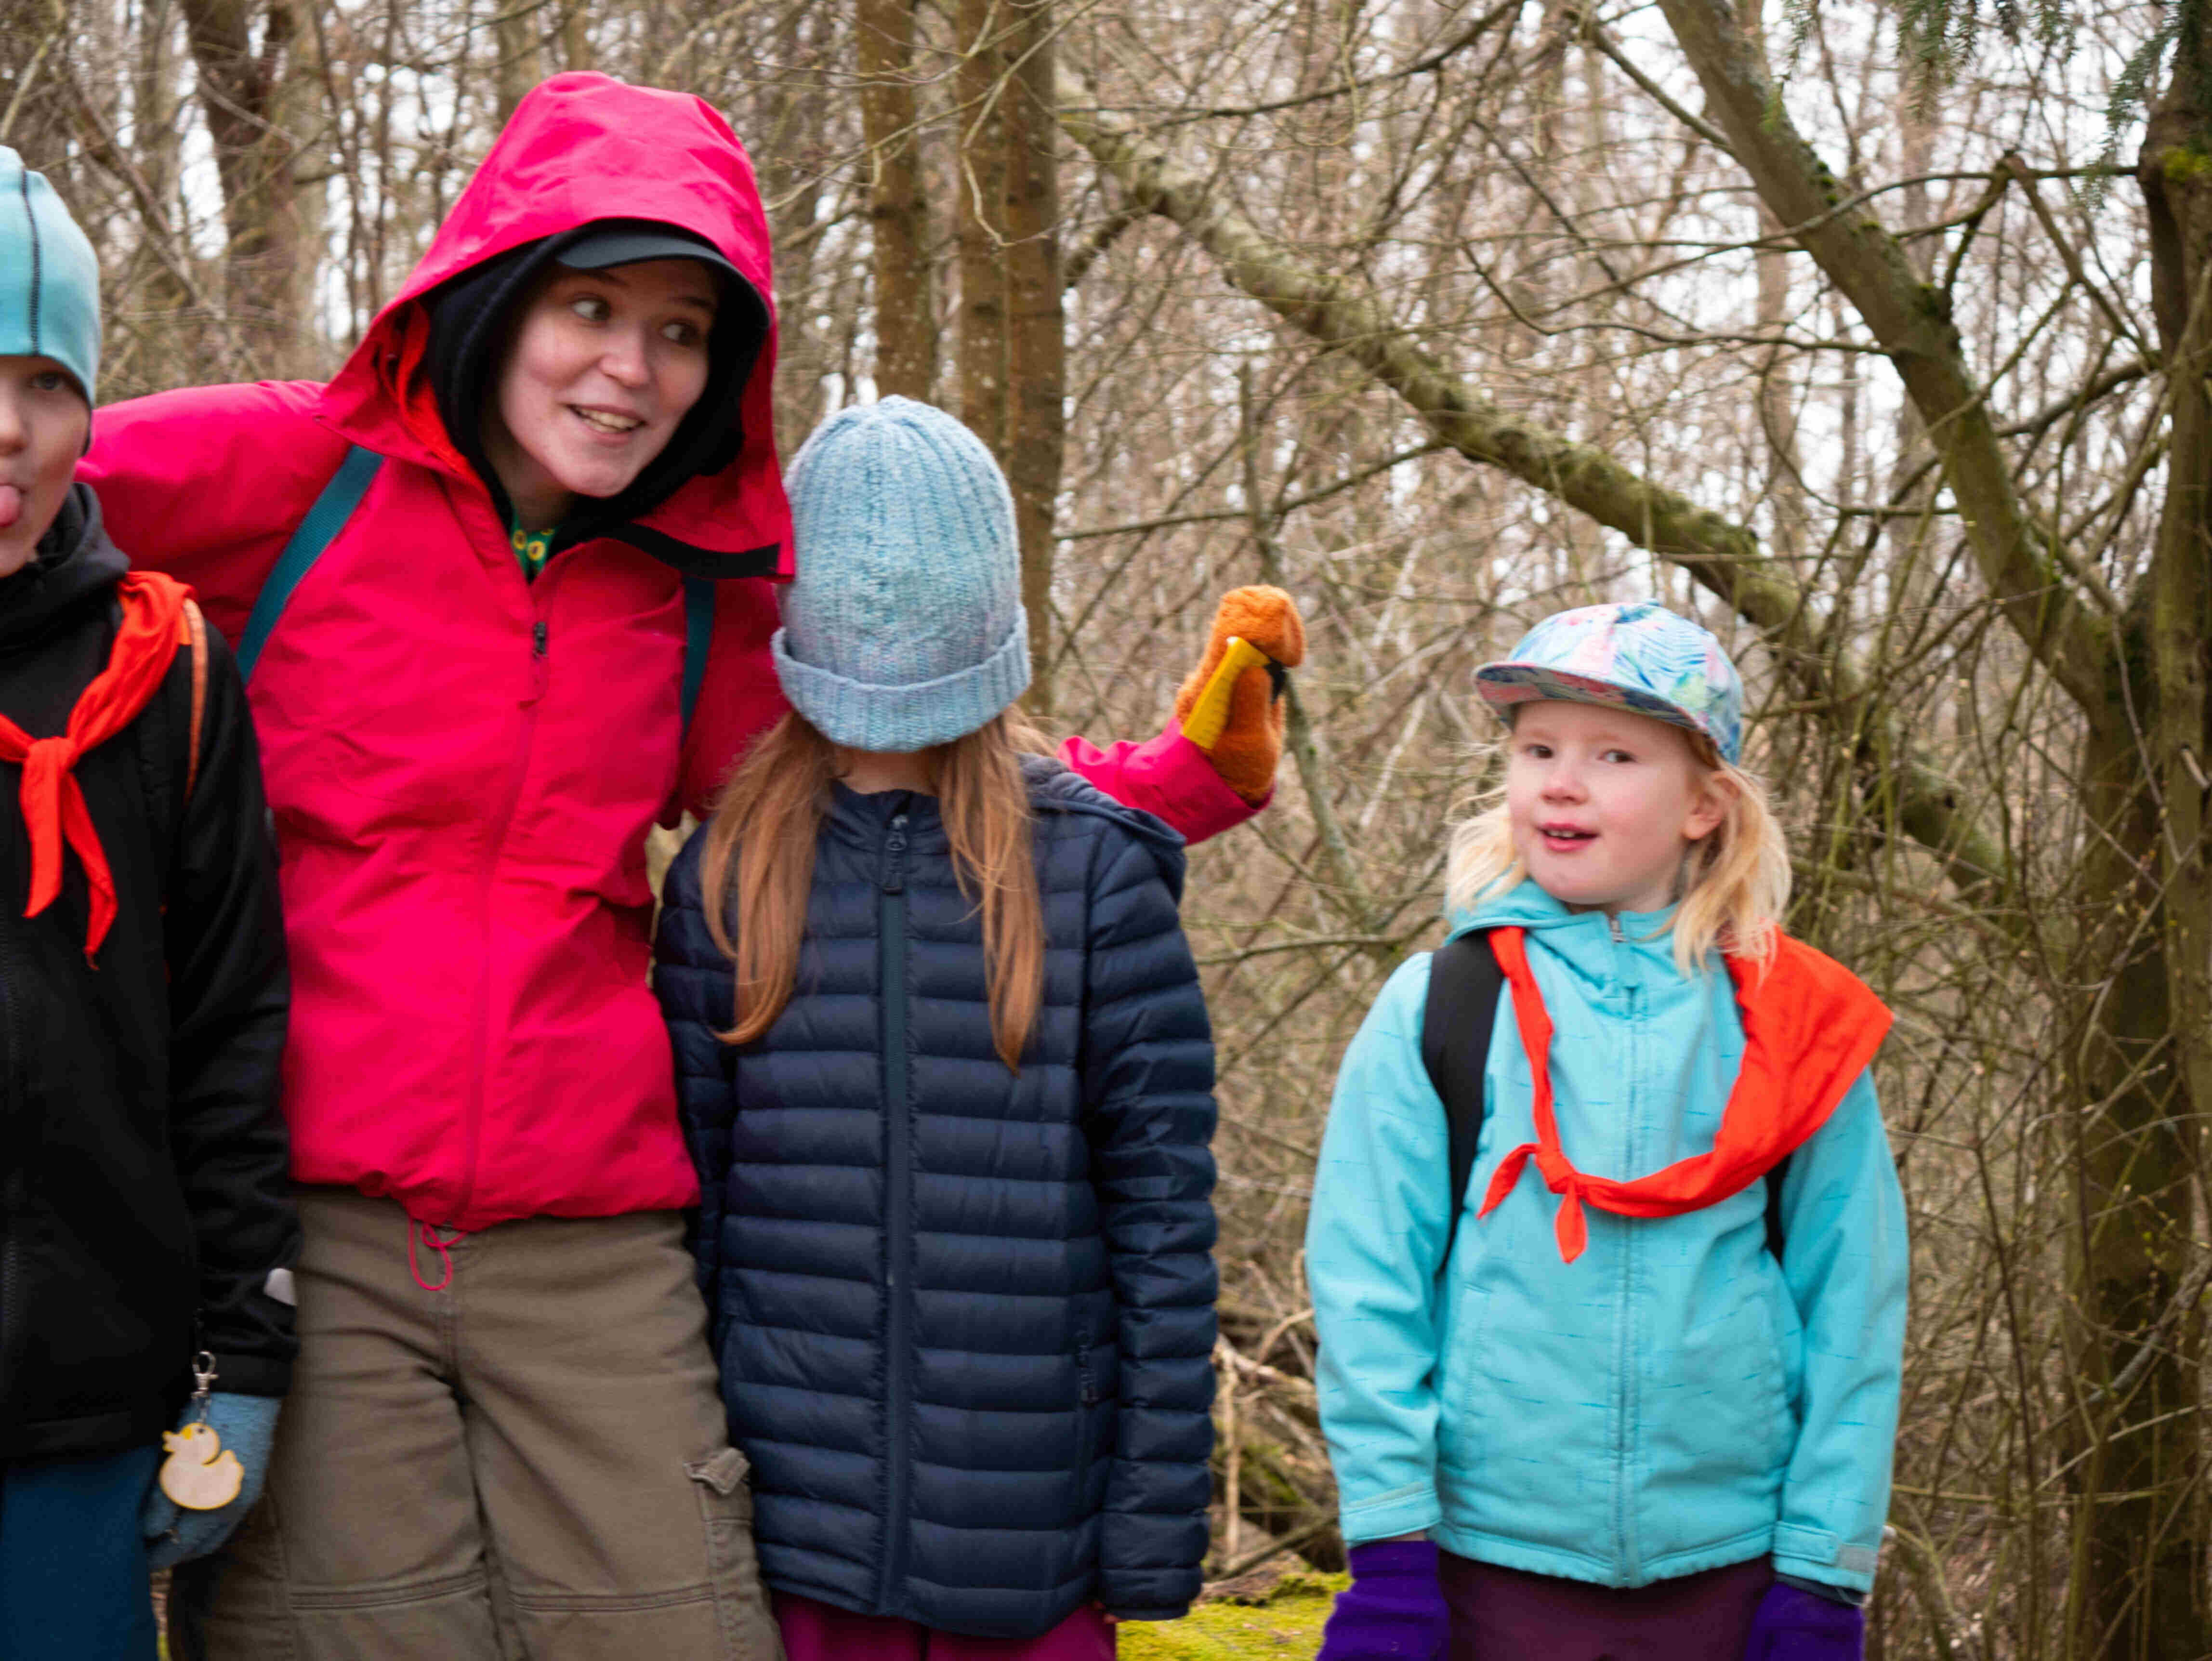
\includegraphics[width=0.9\linewidth]{assets/kolkkienpäiväretki9}
	\noindent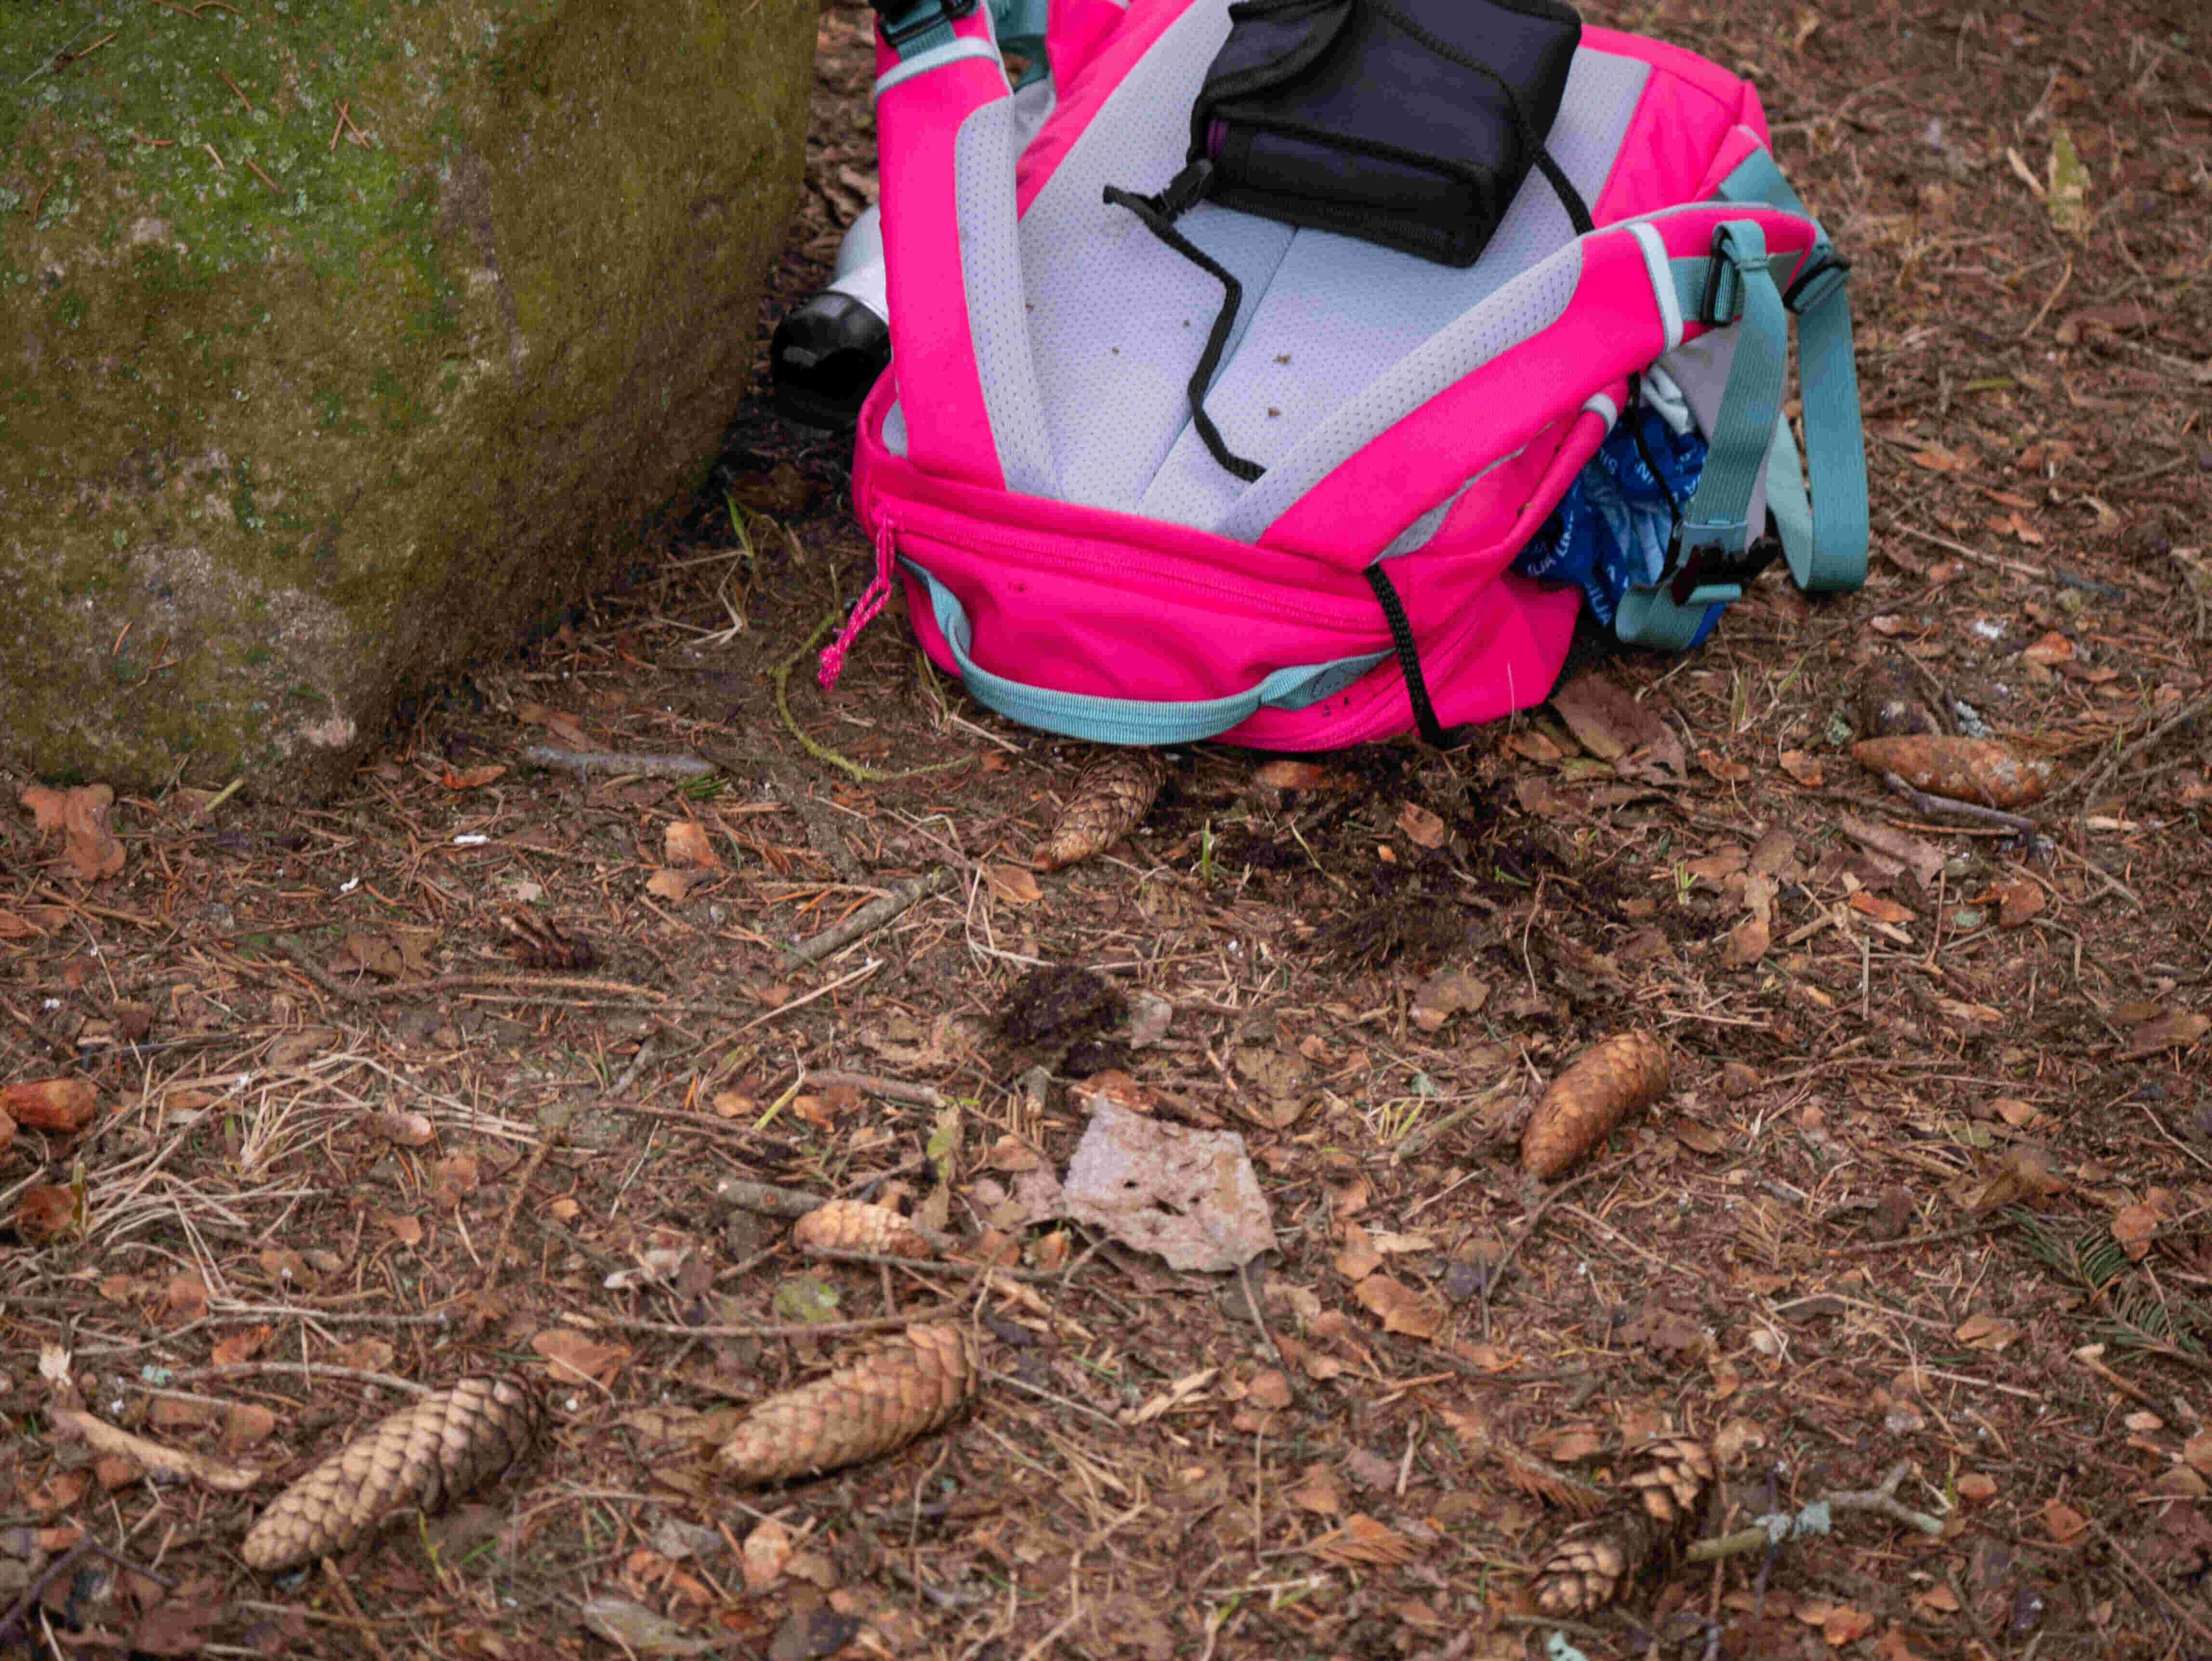
\includegraphics[width=0.9\linewidth]{assets/kolkkienpäiväretki10}
	\noindent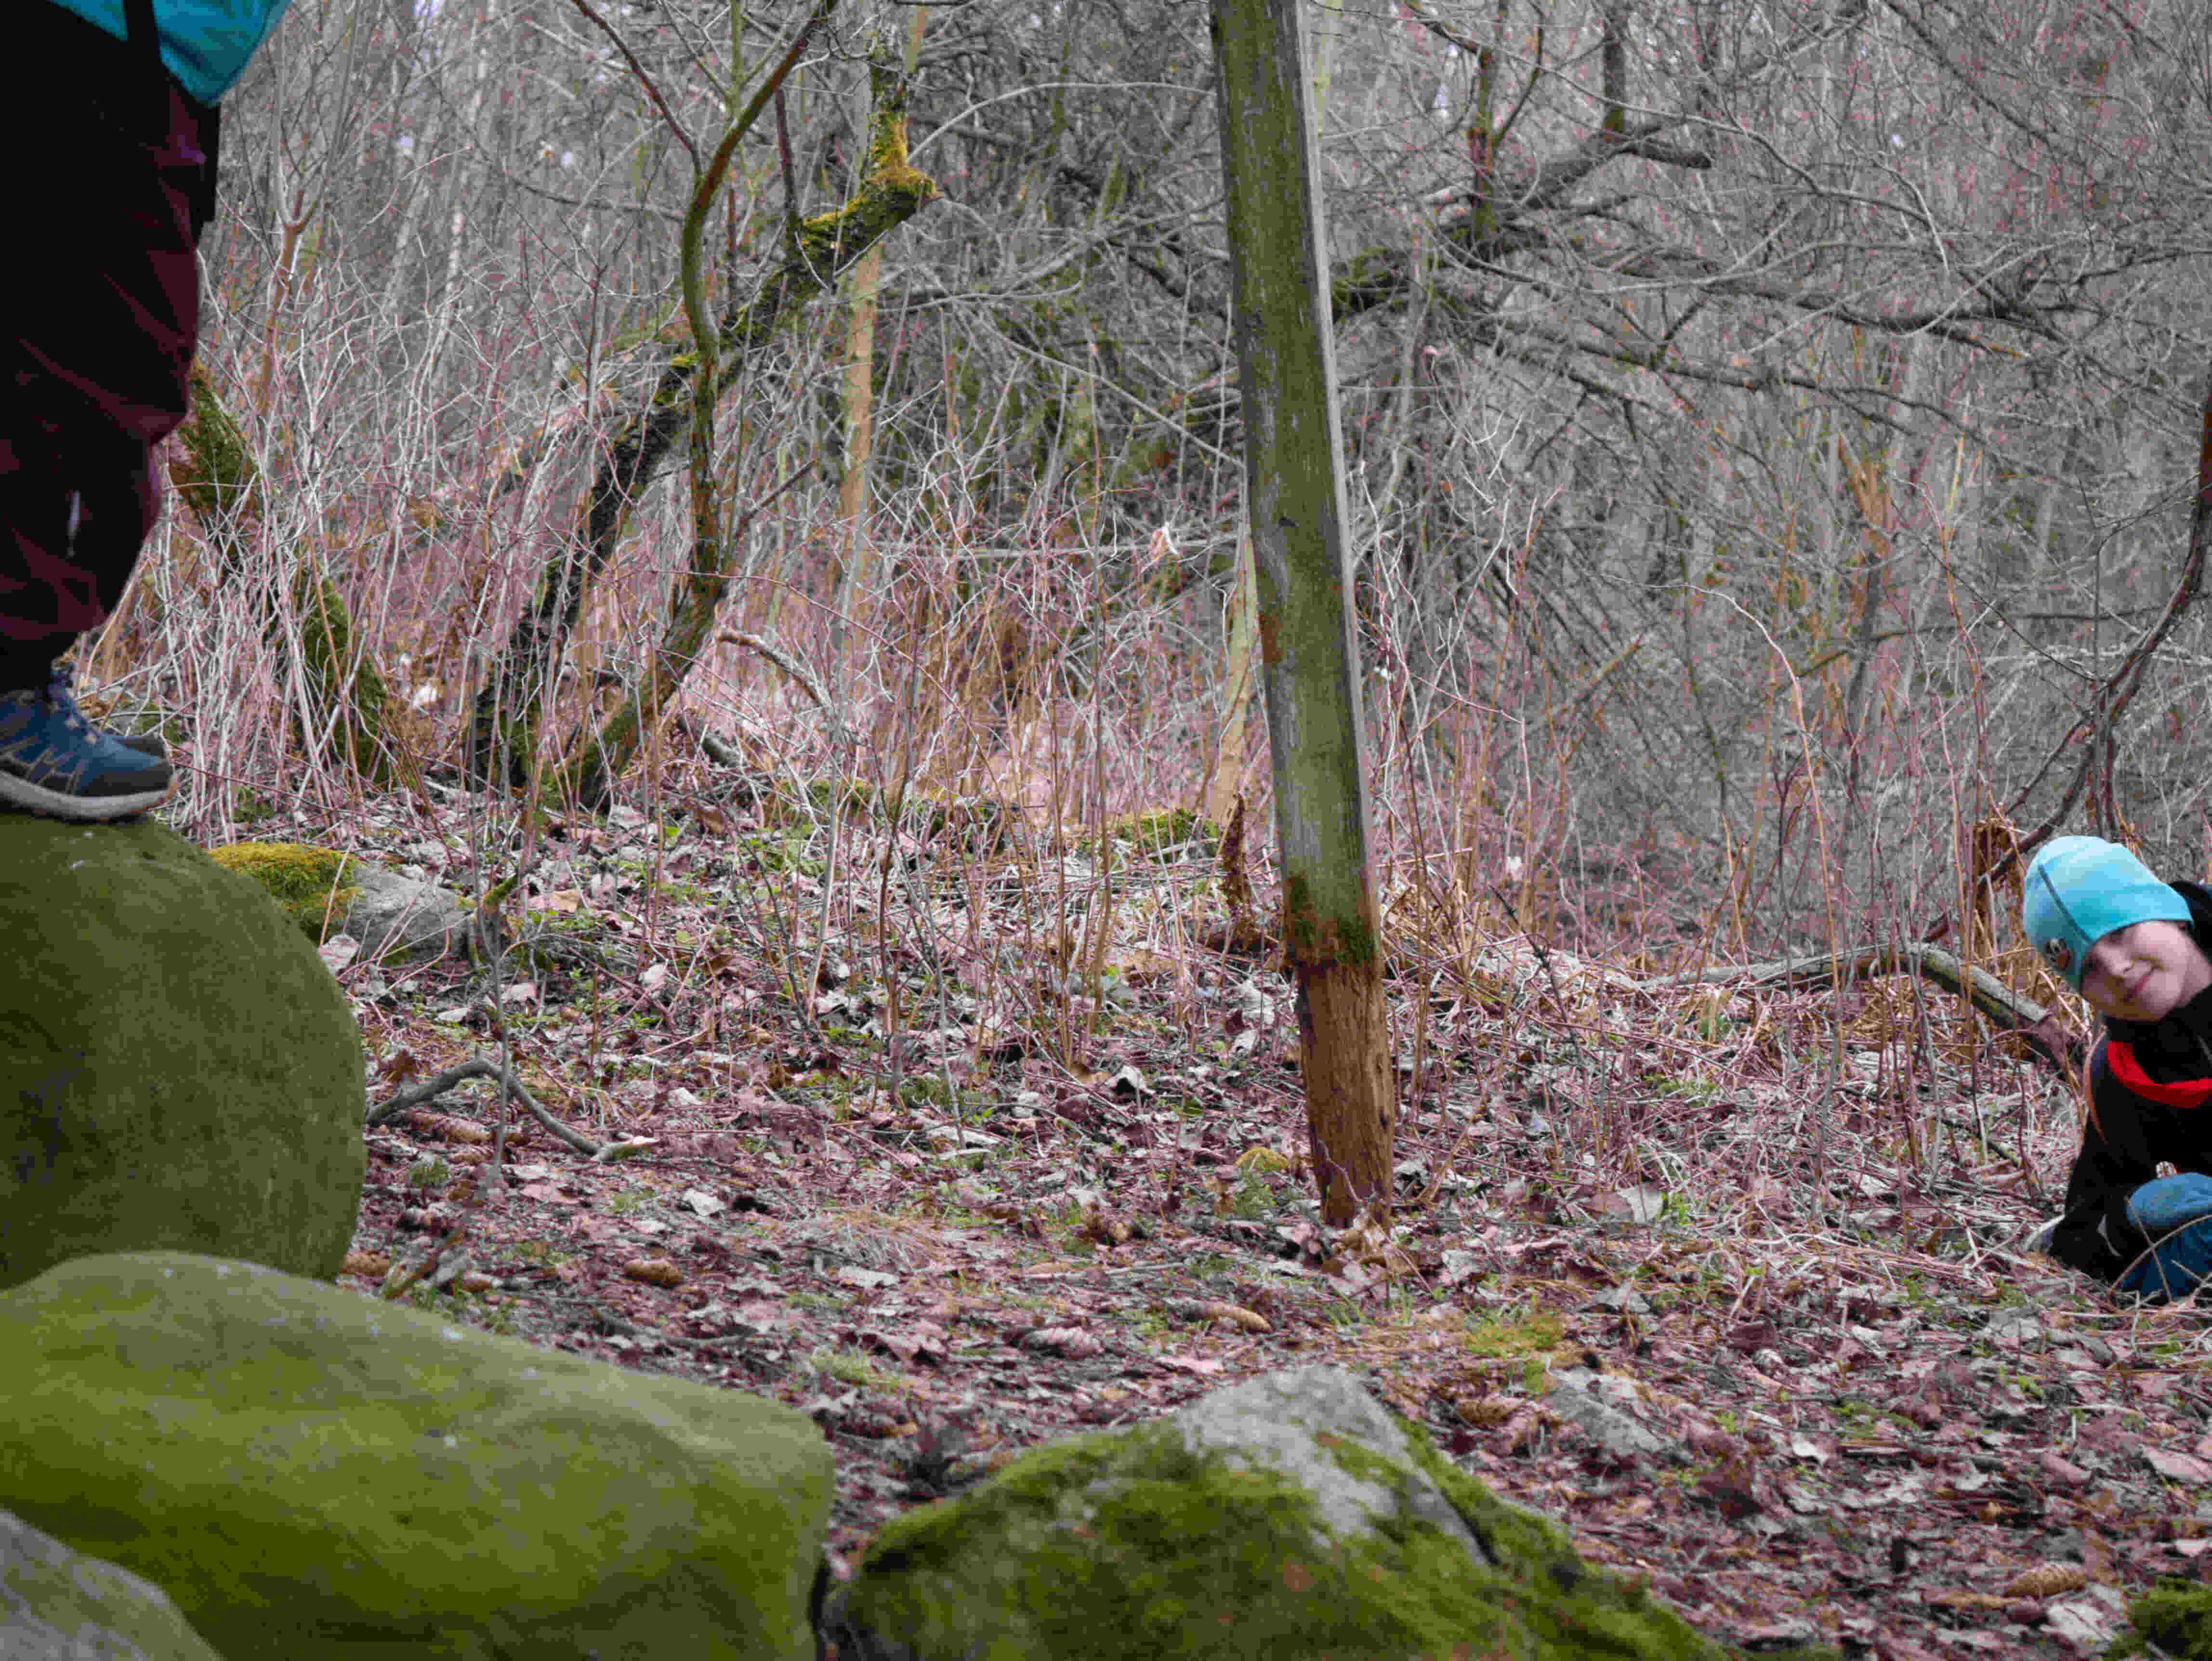
\includegraphics[width=0.9\linewidth]{assets/kolkkienpäiväretki11}
	\noindent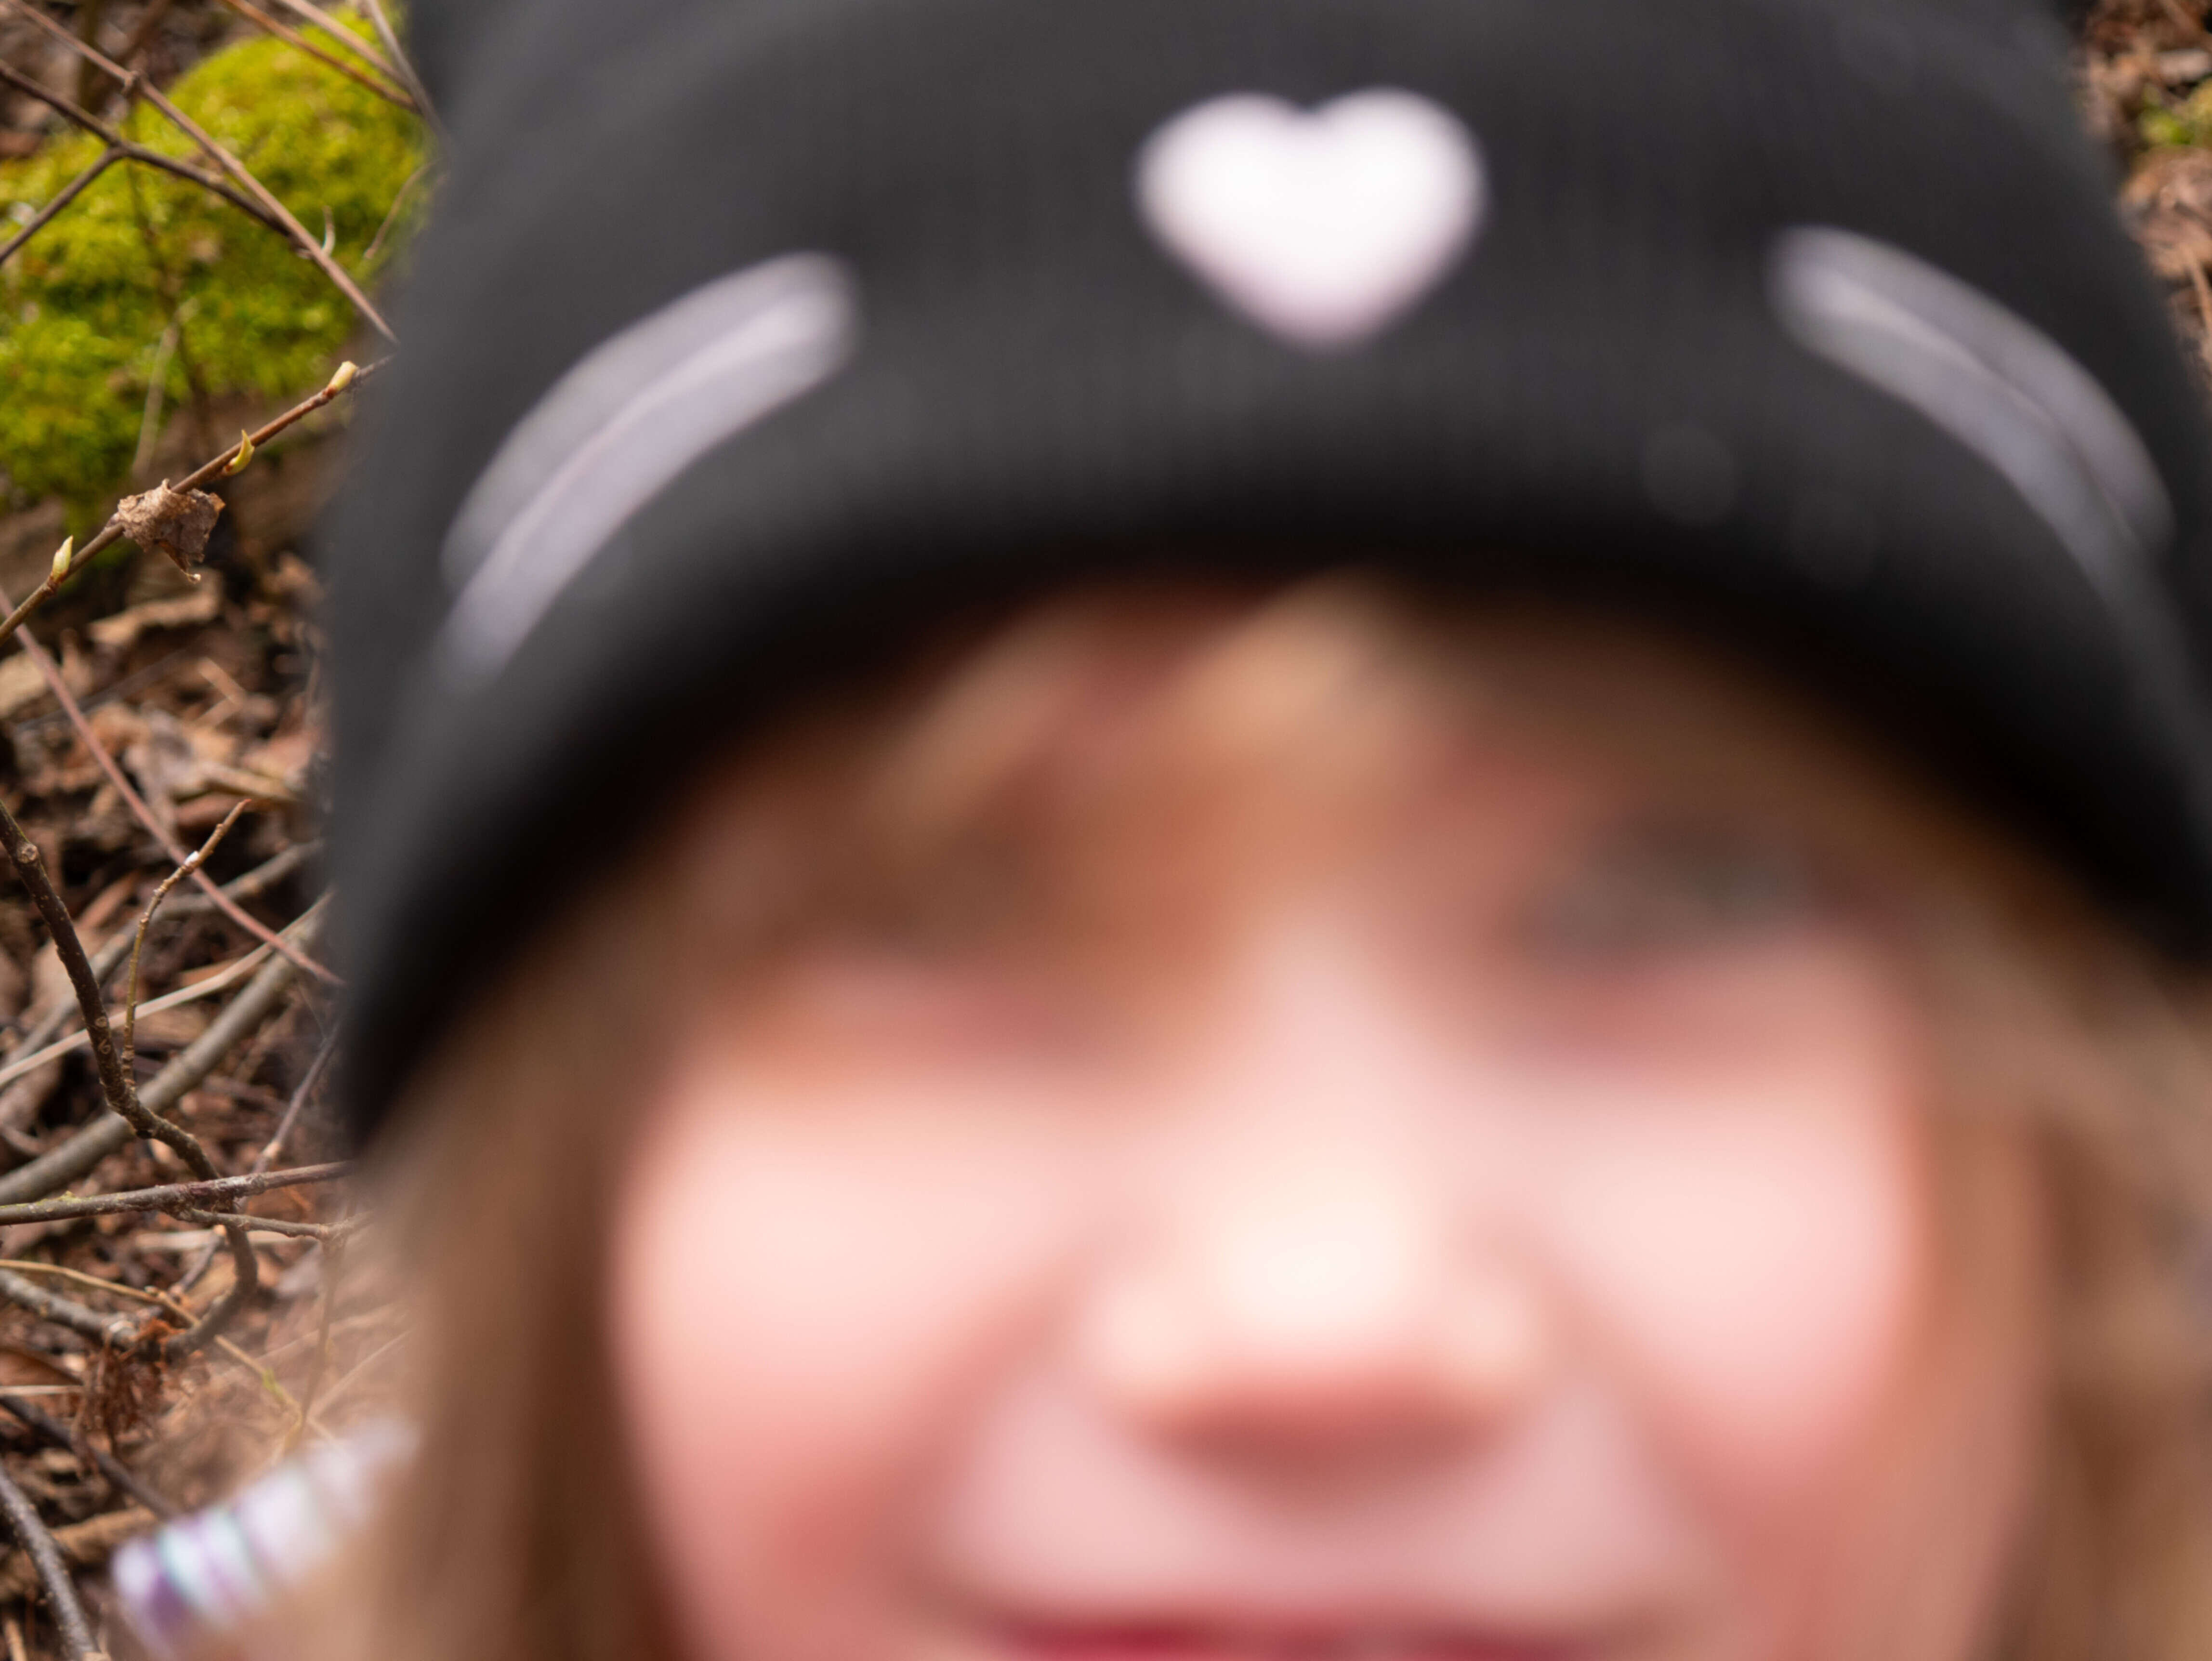
\includegraphics[width=0.9\linewidth]{assets/kolkkienpäiväretki12}

\end{multicols}



\section{Olion paluu 19.--21.4.}

\begin{multicols}{2}

	\noindent Jatkona viime syksyn \textit{Operaatio olio} "=telttaretkelle lippukunnan
	seikkailijavartio \textit{Makkaramokkulat} ja tarpojavartio \textit{Päärynähyttyset} lähtivät
	telttailemaan samoihin Sipoonkorven maastoihin retken jännittävässä jatko"-
	osassa \textit{Olion paluu}, jonka \textit{Vene}"-vartio oli jälleen menestyksekkäästi
	suunnitellut.

	Kaksitoista rusakkoa kokoontui retken lähtöön jo tutussa paikassa,
	Kontulan ostarin Kalkan Pizza"-Kebab"-Grillin edustalla
	perjantai"-iltapäivänä. Kun osa retkeläisistä hyppäsi bussiin kohti
	Viikkiä, osa siirtyi lippukunnan varastolle, jossa logistiikkamestari
	Mikko odotti valmiina hakemaan retken ruoat ja kyyditsemään ne kaluston
	-- ja kantajien -- kanssa telttapaikalle. Bussiosasto jatkoi Viikistä
	Sipoon Myyrakseen. 

	Bussiosastolla oli edessä tuskien taival: 2,4 kilometrin kävely
	pysäkiltä telttapaikan läheiselle parkkipaikalle. Toisaalta, ei
	auto-osastollakaan helppoa ollut kantaa kaikki retken ruoat ja yhteiset
	varusteet parkkipaikalta ylös leiriin. Vaikka matkaa oli vain 700
	metriä, oli leiripaikka viisitoista metriä korkeammalla merenpinnasta
	kuin parkkipaikka. Tehtävästä suoriuduttiin kuitenkin ansiokkaasti.

	Telttapaikalla aloitettiin leirityöt: Osa retkeläisistä alkoi pilkkoa
	puita yötä varten kun taas osa alkoi pystyttää telttaa. Teltan pystytys
	ei sujunut aivan määräajassa, mutta lopputulos oli särmä ja erittäin
	maastokelpoinen -- mitä nyt yhtä kaminan jalkaa etsittiin
	epätoivoisesti, vaikka se oli koko ajan teltan sisällä. Selvästi
	telttaa ei käytetä tarpeeksi, kun kulmasalkojen asentaminen on niin
	paljon voimaa vaativa työ.

	Tässä vaiheessa retkeä alkoi satamaan lunta ja lumentulo jatkuikin aina
	sunnuntaihin asti. Huhtikuista takatalvea ei jääty sen enempää
	ihmettelemään vaan retkeläiset siirtyivät teltan suojaan, jossa kamina
	syttyi melkein itsestään etukäteen valmisteltujen sytykkeiden avulla. 

	\vspace*{0.16cm}
	\noindent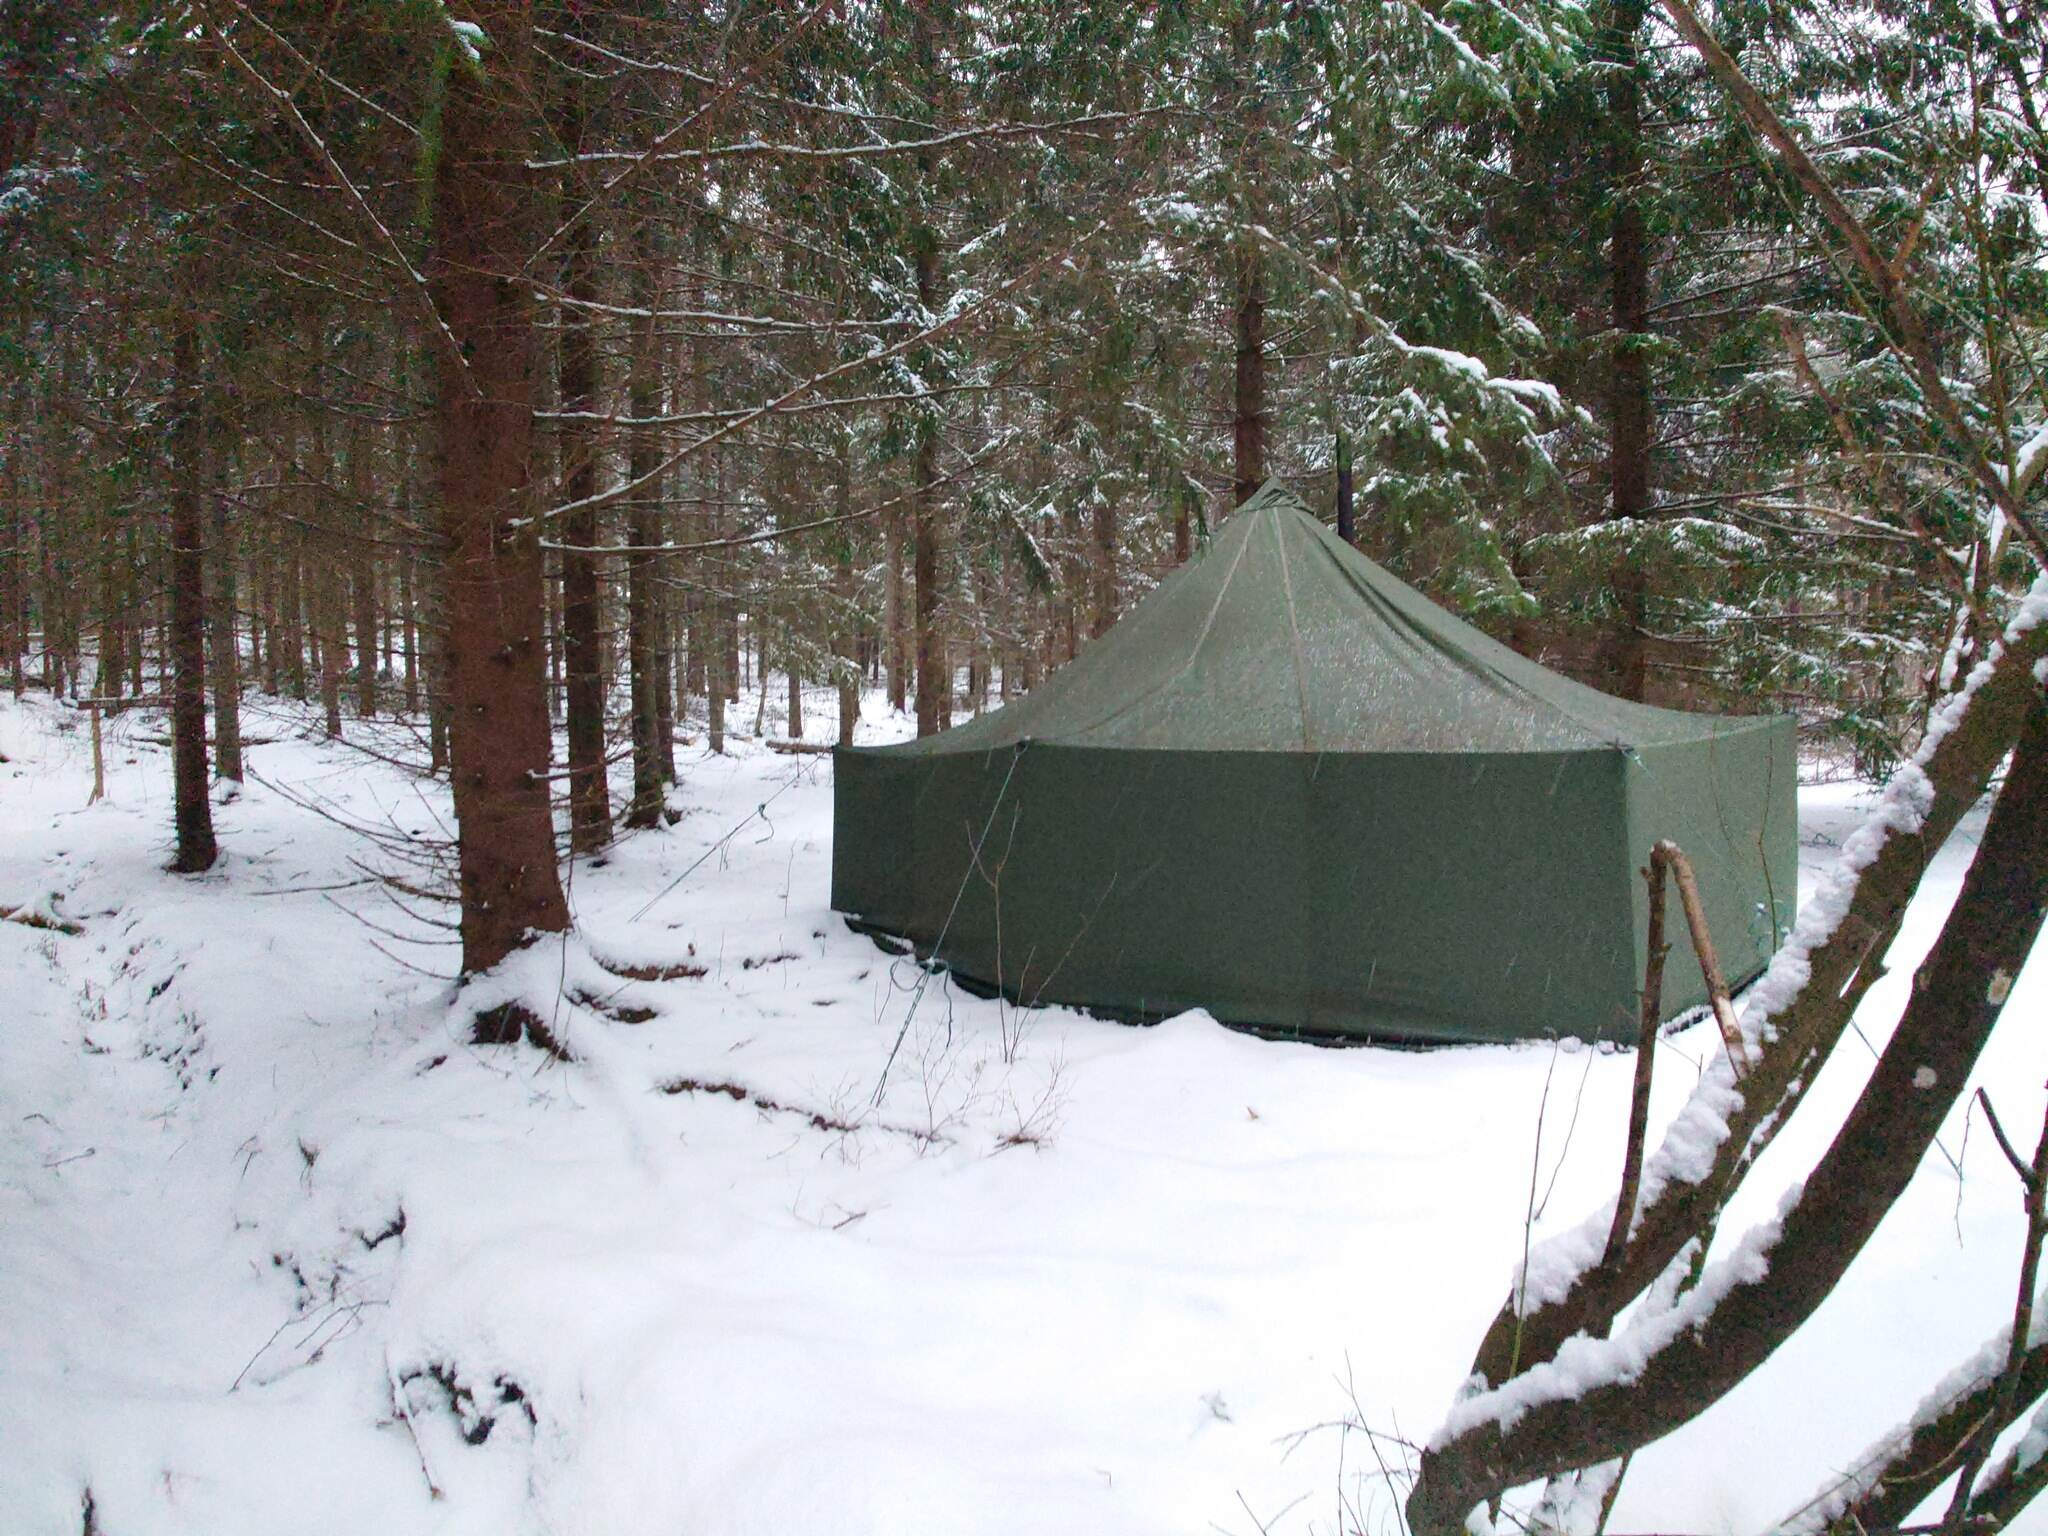
\includegraphics[width=\linewidth]{assets/olionpaluu2}

	Ennen nukkumaanmenoa sovittiin vielä kipinävuoroista: Ensimmäisinä
	kipinävuorossa valvoivat Elias ja Mikael, sitten Alden ja Toivo,
	Joella, Ninni ja Tesla, Ahti ja Kata, Johannes ja Touko, sekä
	viimeisenä Janne. ''Pakastaja Elvi'' ei päässyt yllättämään, vaikka
	kaminaa poltettiinkin säästöliekillä. Ainakin yhden kerran yön aikana
	''lohikäärme'' tuli kuitenkin tarpeeseen, kun kyteville puille piti antaa
	vähän lisäilmaa. Niin ikään osalla retkeläisistä oli aamuksi
	jännitystä, kun Ahti pisti pystyyn F1"-kisastudion.

	\vspace*{0.16cm}
	\noindent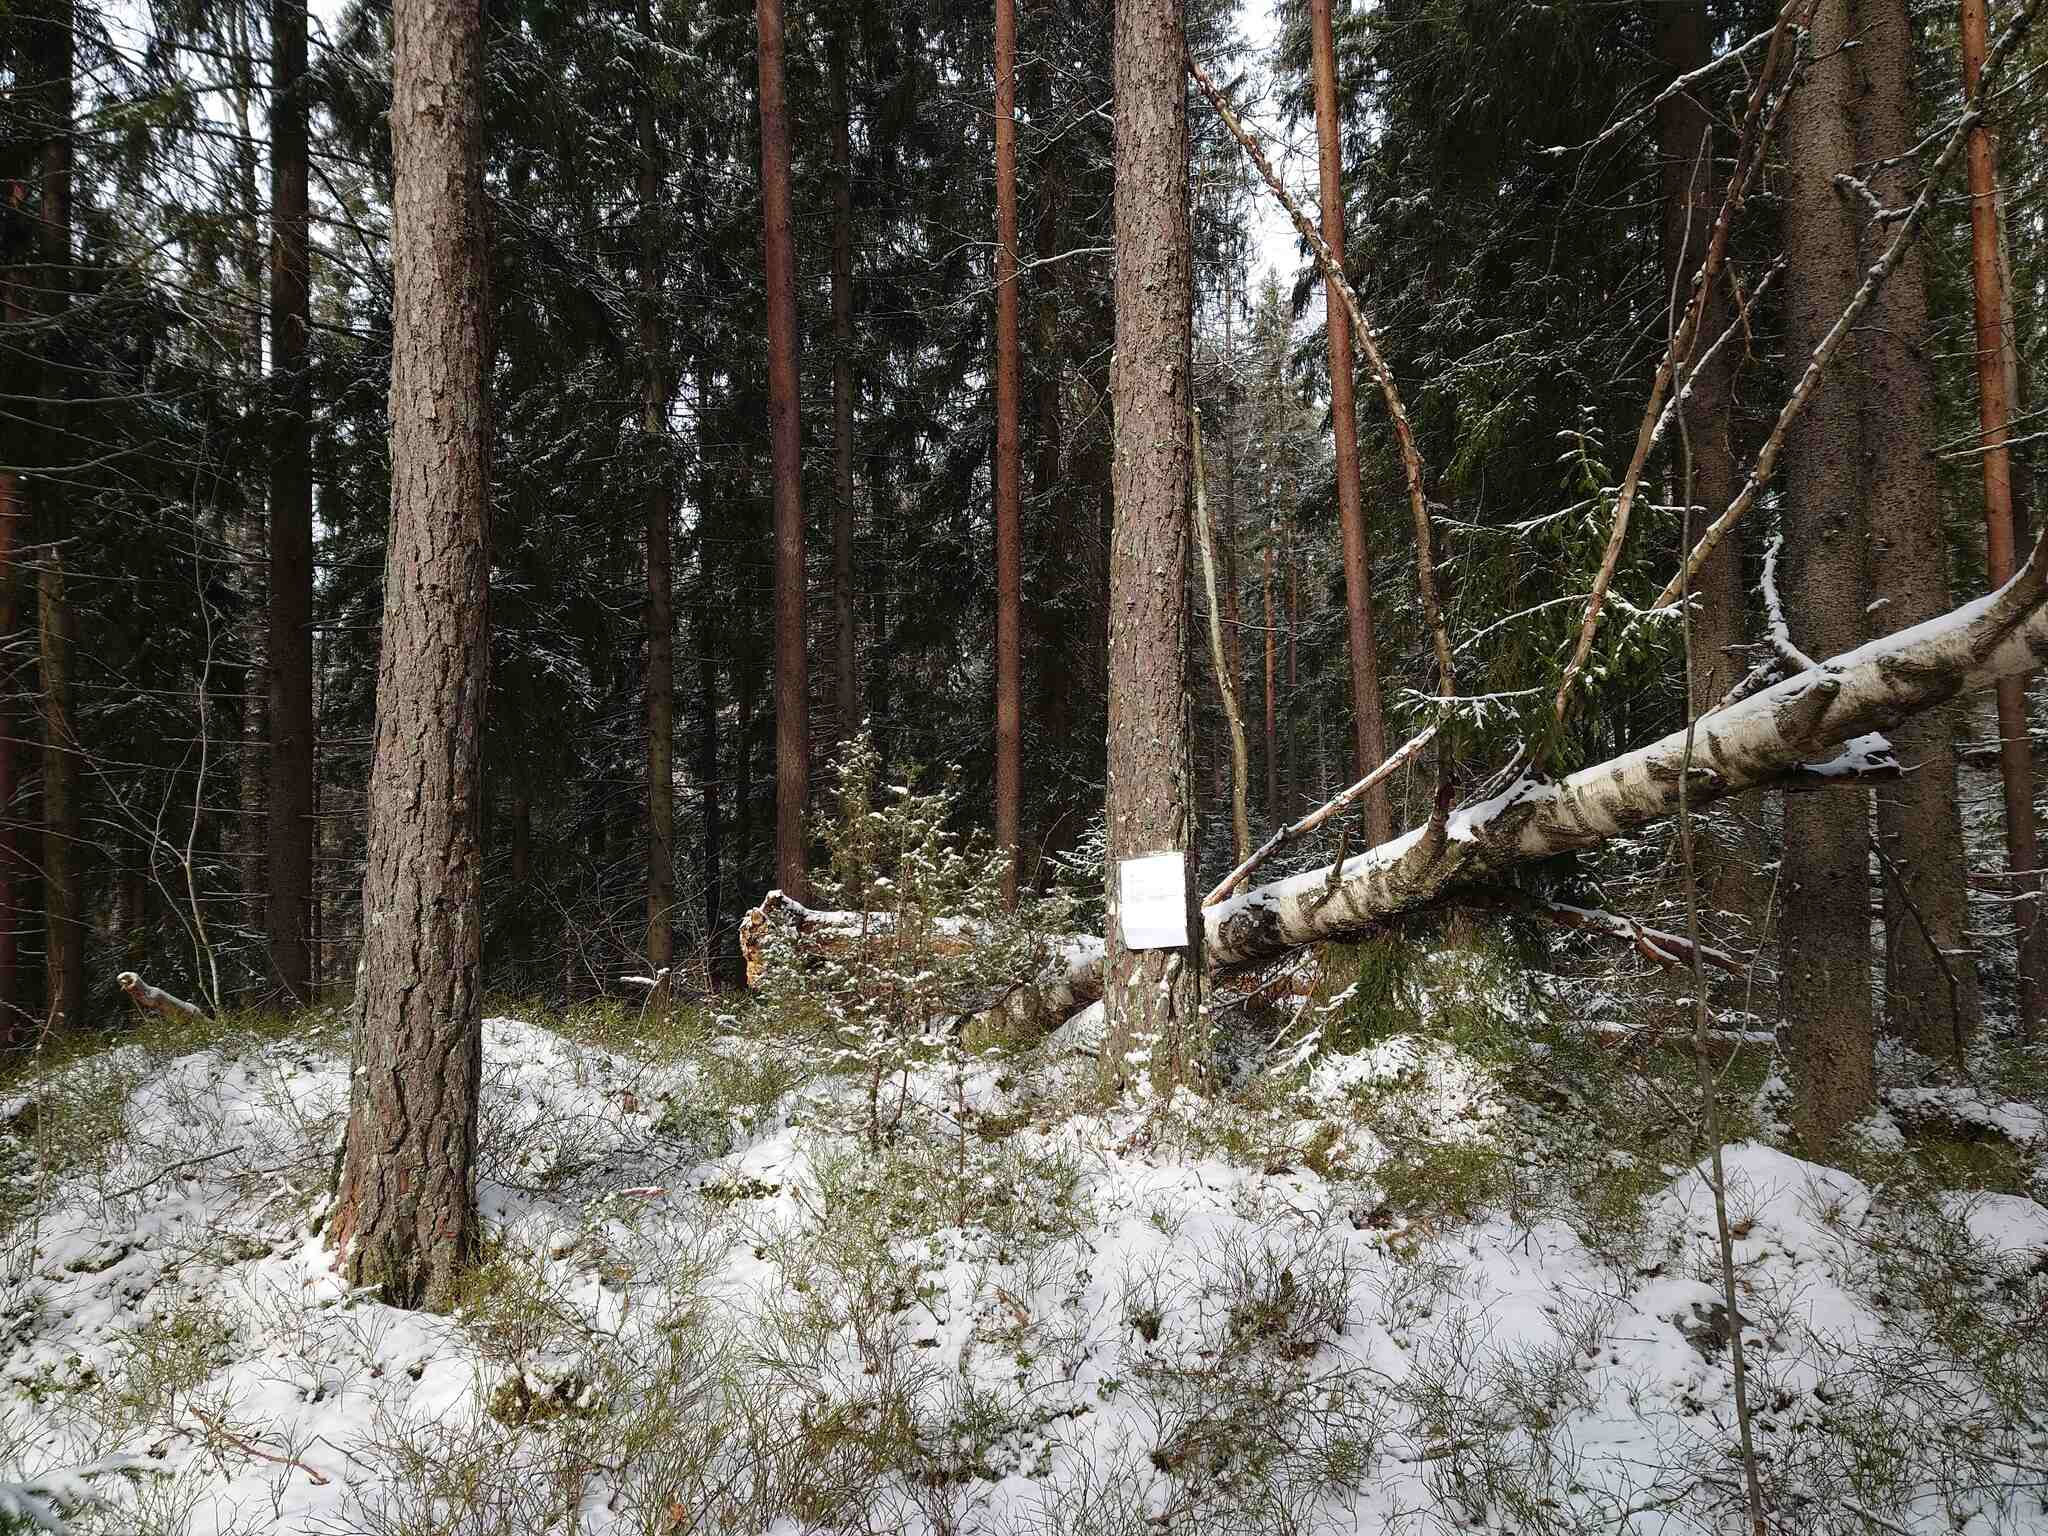
\includegraphics[width=\linewidth]{assets/olionpaluu4}

	Retkeläiset heräsivät valkeaan lauantaiaamuun: lunta oli tullut yön
	aikana useampi sentti ja lämpötila oli muutaman asteen pakkasen
	puolella. Väsyneet ja kohmeiset retkeläiset siirtyivät aamupuuron
	pariin. Ravittuina leikittiin sitten Katan johdolla kaikkien
	suosikkileikkejä kuten pölkkyä ja tervapataa -- jälkimmäistä tosin
	vahvasti kontaktiversiona. 

	Ja taas syötiin: trangioilla valmistui maukasta tonnikalanuudelia ja
	tofunuudelia. Onnistuipa osa retkeläisistä kastelemaan kenkänsä
	nuotiopaikan lätäkössä. Siis vatsat täynnä ja kenkä märkänä aloitettiin
	retken juoneen liittyvä suunnistus. Viiden rastin viuhkasuunnistuksessa
	oli kolme miehitettyä ja kaksi kylmää rastia. Kullakin rastilla
	vartioiden suoritukset pisteytettiin niin käpyjen keräämisessä,
	eläinten jälkien tunnistamisessa, näyttelijän taidoissa, ryhmäkuvan
	ottamisessa kuin laskuvarjon rakentamisessakin. Kultakin rastilta
	selvisi myös vihjeitä salaperäisestä oliosta. 

	Kuten pistetaulukosta voit tarkistaa, pistekilpailun voittajaksi
	selvisi yhden pisteen erolla Minä ja toi "=vartio -- onnittelut!

	Suunnistuksen jälkeen käytiin juoni nopeasti yhdessä läpi ja puolet
	retkeläisistä lähti maitojunalla kotiin. Jäljelle jääneet pilkkoivat
	lisää puita yötä varten ja lämmittivät itselleen kolme kattilallista
	hernekeittoa, joka saatiin melkein kokonaan viiteen pekkaan syötyä!

	\vspace*{0.08cm}
	\noindent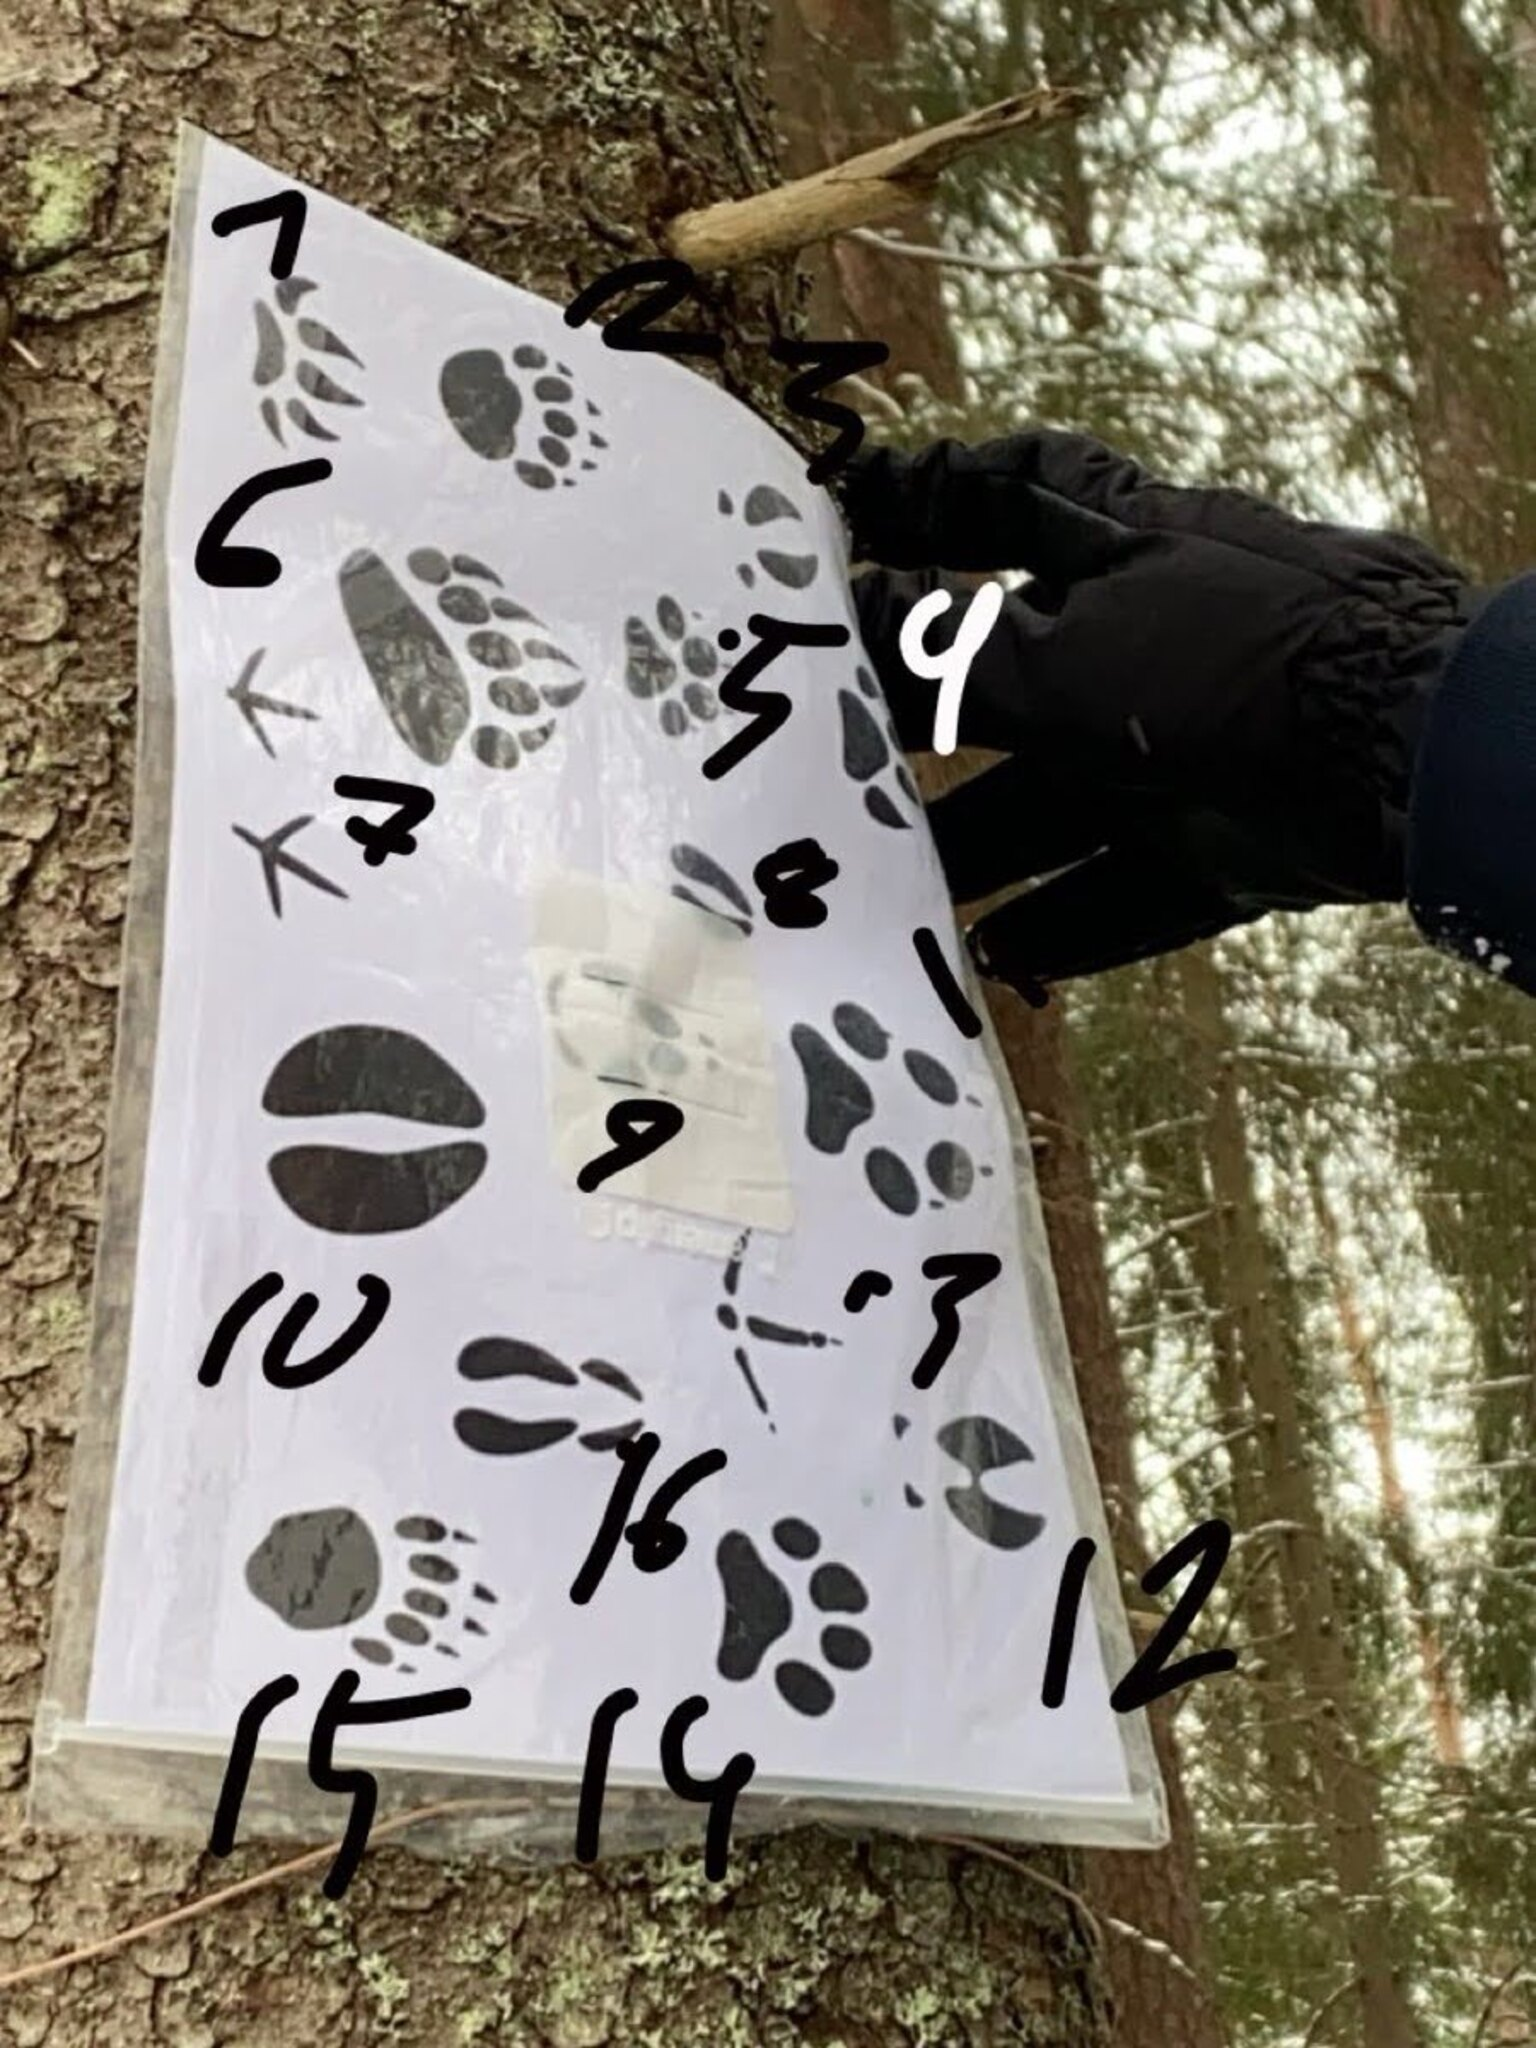
\includegraphics[width=\linewidth]{assets/olionpaluu3}

	Kaikki oli valmista yötä varten. Kello ei ollut vielä kahdeksaakaan,
	mutta retkue päätti siirtyä jo telttaan lämmittelemään ja
	kuivattelemaan varusteita -- ja sivuun telttapaikalle tulleilta muiden
	lippukuntien ryhmänohjaajakoulutettavilta, jotka myös olivat yöpymässä
	puolijoukkueteltalla. Kaminaa poltettiin vähän isommalla liekillä kuin
	ensimmäisenä yönä ja teltan lämmetessä alkoi itse kullakin silmäluomi
	painaa. Kipinävuoroista sovittiin, että ensimmäisenä valvoi Ahti,
	sitten Elias ja viimeisenä Janne. 

	\vspace*{0.08cm}
	\noindent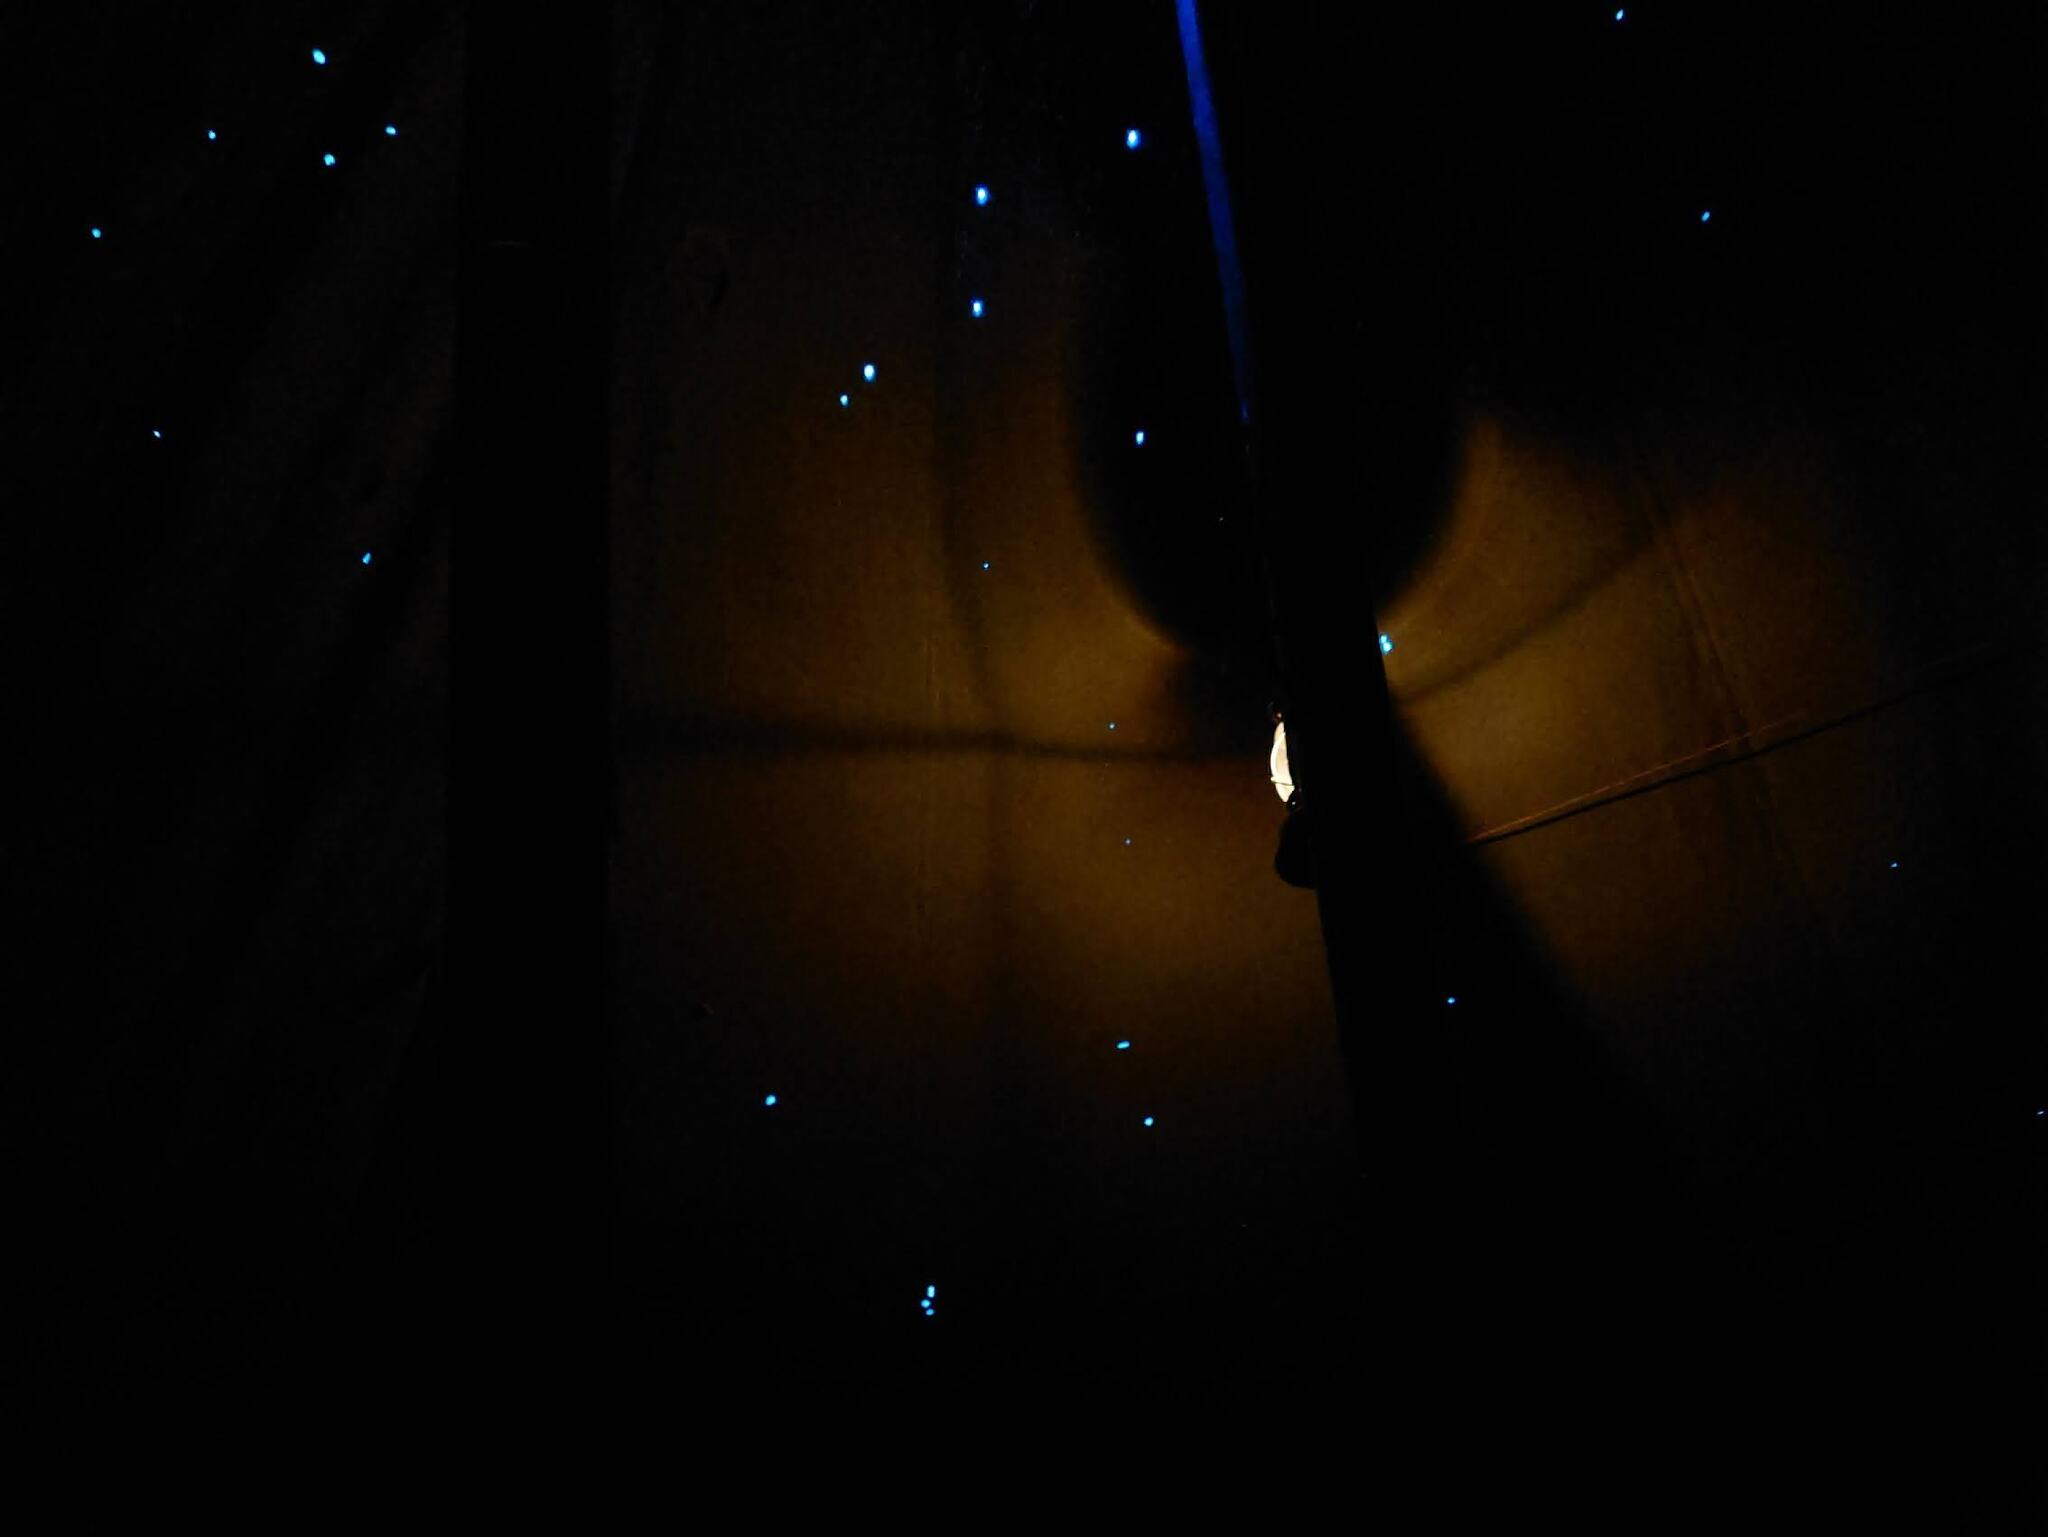
\includegraphics[width=\linewidth]{assets/olionpaluu1}

	Aamu alkoi reippaasti puuroveden kiehuessa kaminan päällä, kun teltan
	sisällä ei ollut tietoakaan ulkoilman kylmyydestä tai kosteudesta.
	Varusteet pakattiin vauhdikkaasti ja teltta pistettiin kasaan. Kaminan
	piippu oli yhdestä kohtaa niin tiukassa, että sen irroittamisessa meni
	tovi. Siitä huolimatta piipun palat saatiin sovitettua siististi
	kaminan sisälle (toim. huom. jotain, jossa allekirjoittanut epäonnistui
	surkeasti varastolla perjantaina).

	Kalustoa alettiin roudata takaisin parkkipaikalle. Alamäkeen kantaminen
	sujui vähän helpommin, mutta märkä teltta oli raskas ja polku paikoin
	liukas. Mikko olikin tullut parahiksi parkkipaikalle vastaan ja auto
	pakattiin kalustolla ja retkeläisillä. Hienosti mahtuivat kaikki mukaan
	ja kotimatka voi alkaa.

	Jää nähtäväksi, palaako olio vielä kolmannen kerran. Joka tapauksessa,
	jos viime syksynä satoi vettä kaatamalla ja nyt keväällä oli takatalvi,
	ei seuraavalle kerralle ole enää kovin montaa sään tuomaa haastetta
	jäljellä!

\end{multicols}

\vspace*{0.64cm}
\makebox[0.94\textwidth][c]{%
	\begin{tabular}{ l p{2cm} |r| r r r r r r }
		&&& \textbf{Rasti 2} & \textbf{Rasti 3} & \textbf{Rasti 4} & \textbf{Rasti 5} & \textbf{Rasti 6} & \textbf{Käytös} \\
		& Maks. & 62 & 10 & 17 & 10 & 10 & 15 \\
		\textbf{Sij.} & \textbf{Vartio} & \textbf{Yht.} \\
		\hline
		\textbf{1} & \textit{Minä ja toi}\newline Johannes ja Tesla & 42 & 10 & 8 & 6 & 7 & 11 & 0 \\
		\hline
		\textbf{2} & \textit{TT}\newline Toivo ja Touko & 41 & 10 & 5 & 8 & 7 & 11 & 0 \\
		\hline
		\textbf{3} & Alden ja Joella & 33 & 4 & 6 & 2 & 9 & 11 & 1 \\
	\end{tabular}%
}

\vspace*{0.64cm}
{\raggedleft Kuvat: Retkeläiset \& Janne Suomalainen\\ Teksti: Janne Suomalainen\\}





\clearpage
\subsection{Partioparaati 28.4.}

\vspace*{-0.32cm}
\begin{multicols}{2}

	\begin{center}
		\noindent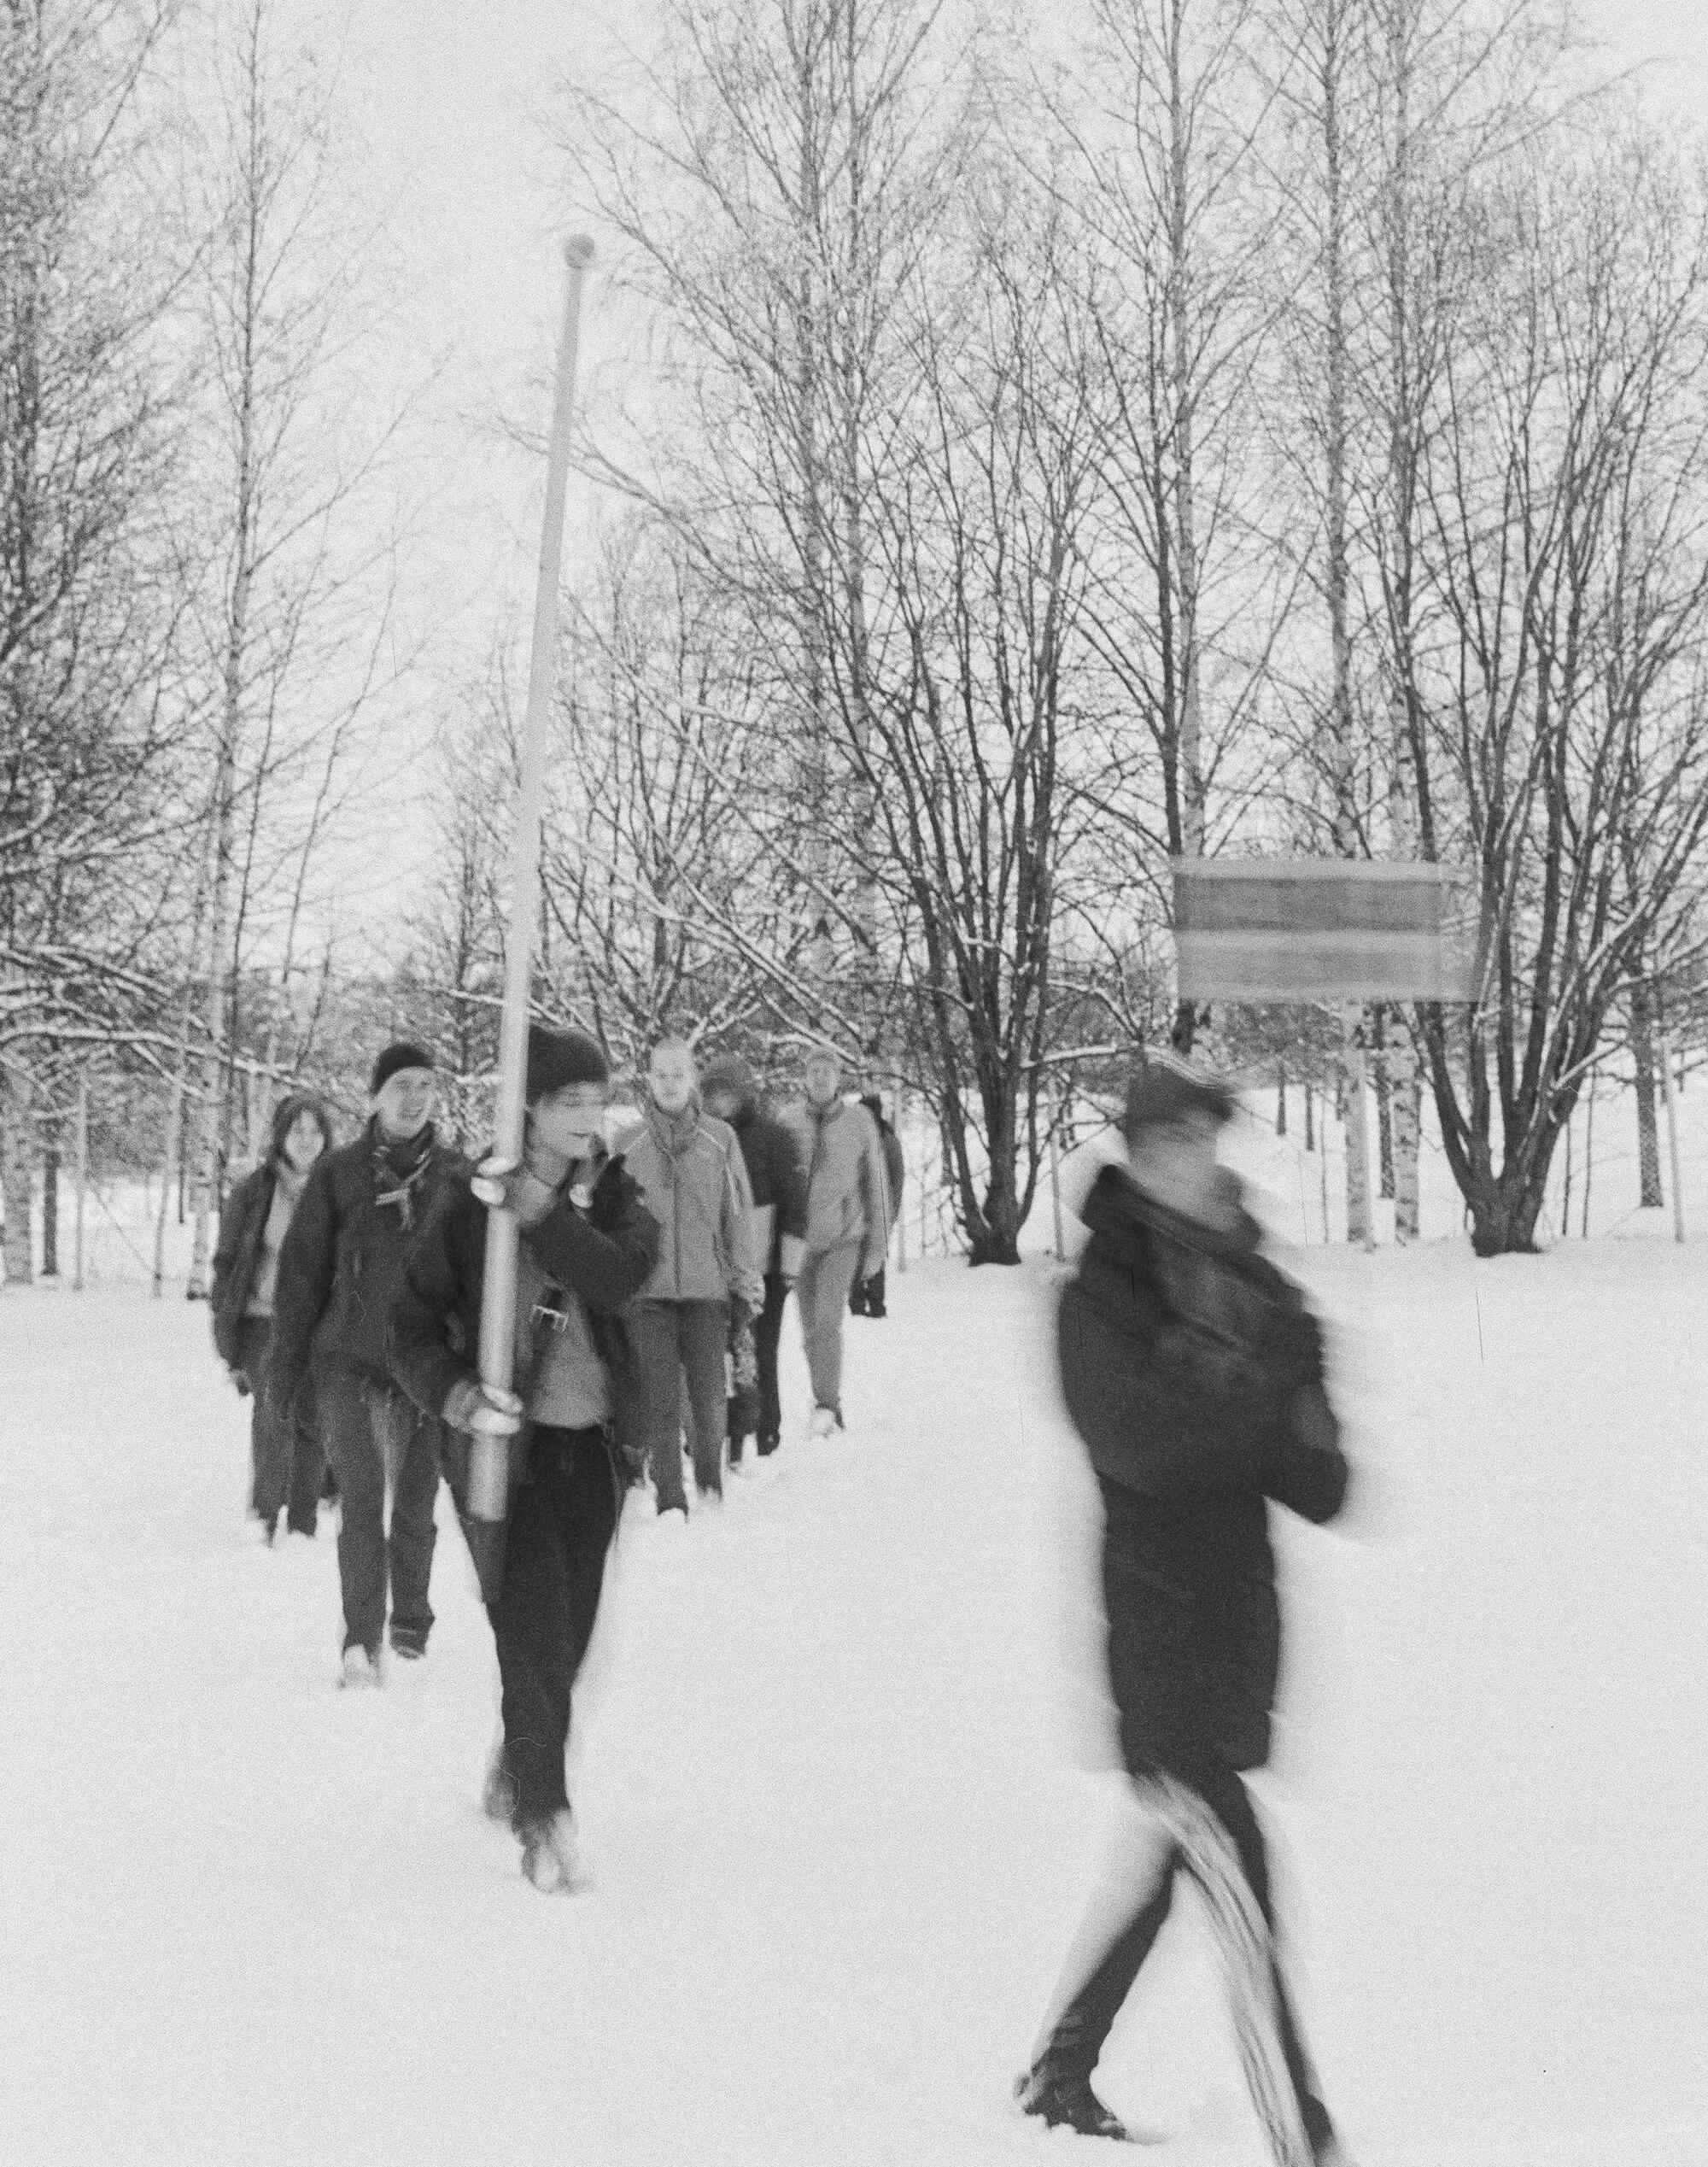
\includegraphics[width=0.9\linewidth]{assets/paraati1}
	\end{center}

	\vspace*{-0.32cm}
	\small KuRu:n paraatiosasto harjoiteli \mbox{paraati}protokollan
	viikkokokouksessa, vielä talvella säällä \ldots

	\begin{center}
		\noindent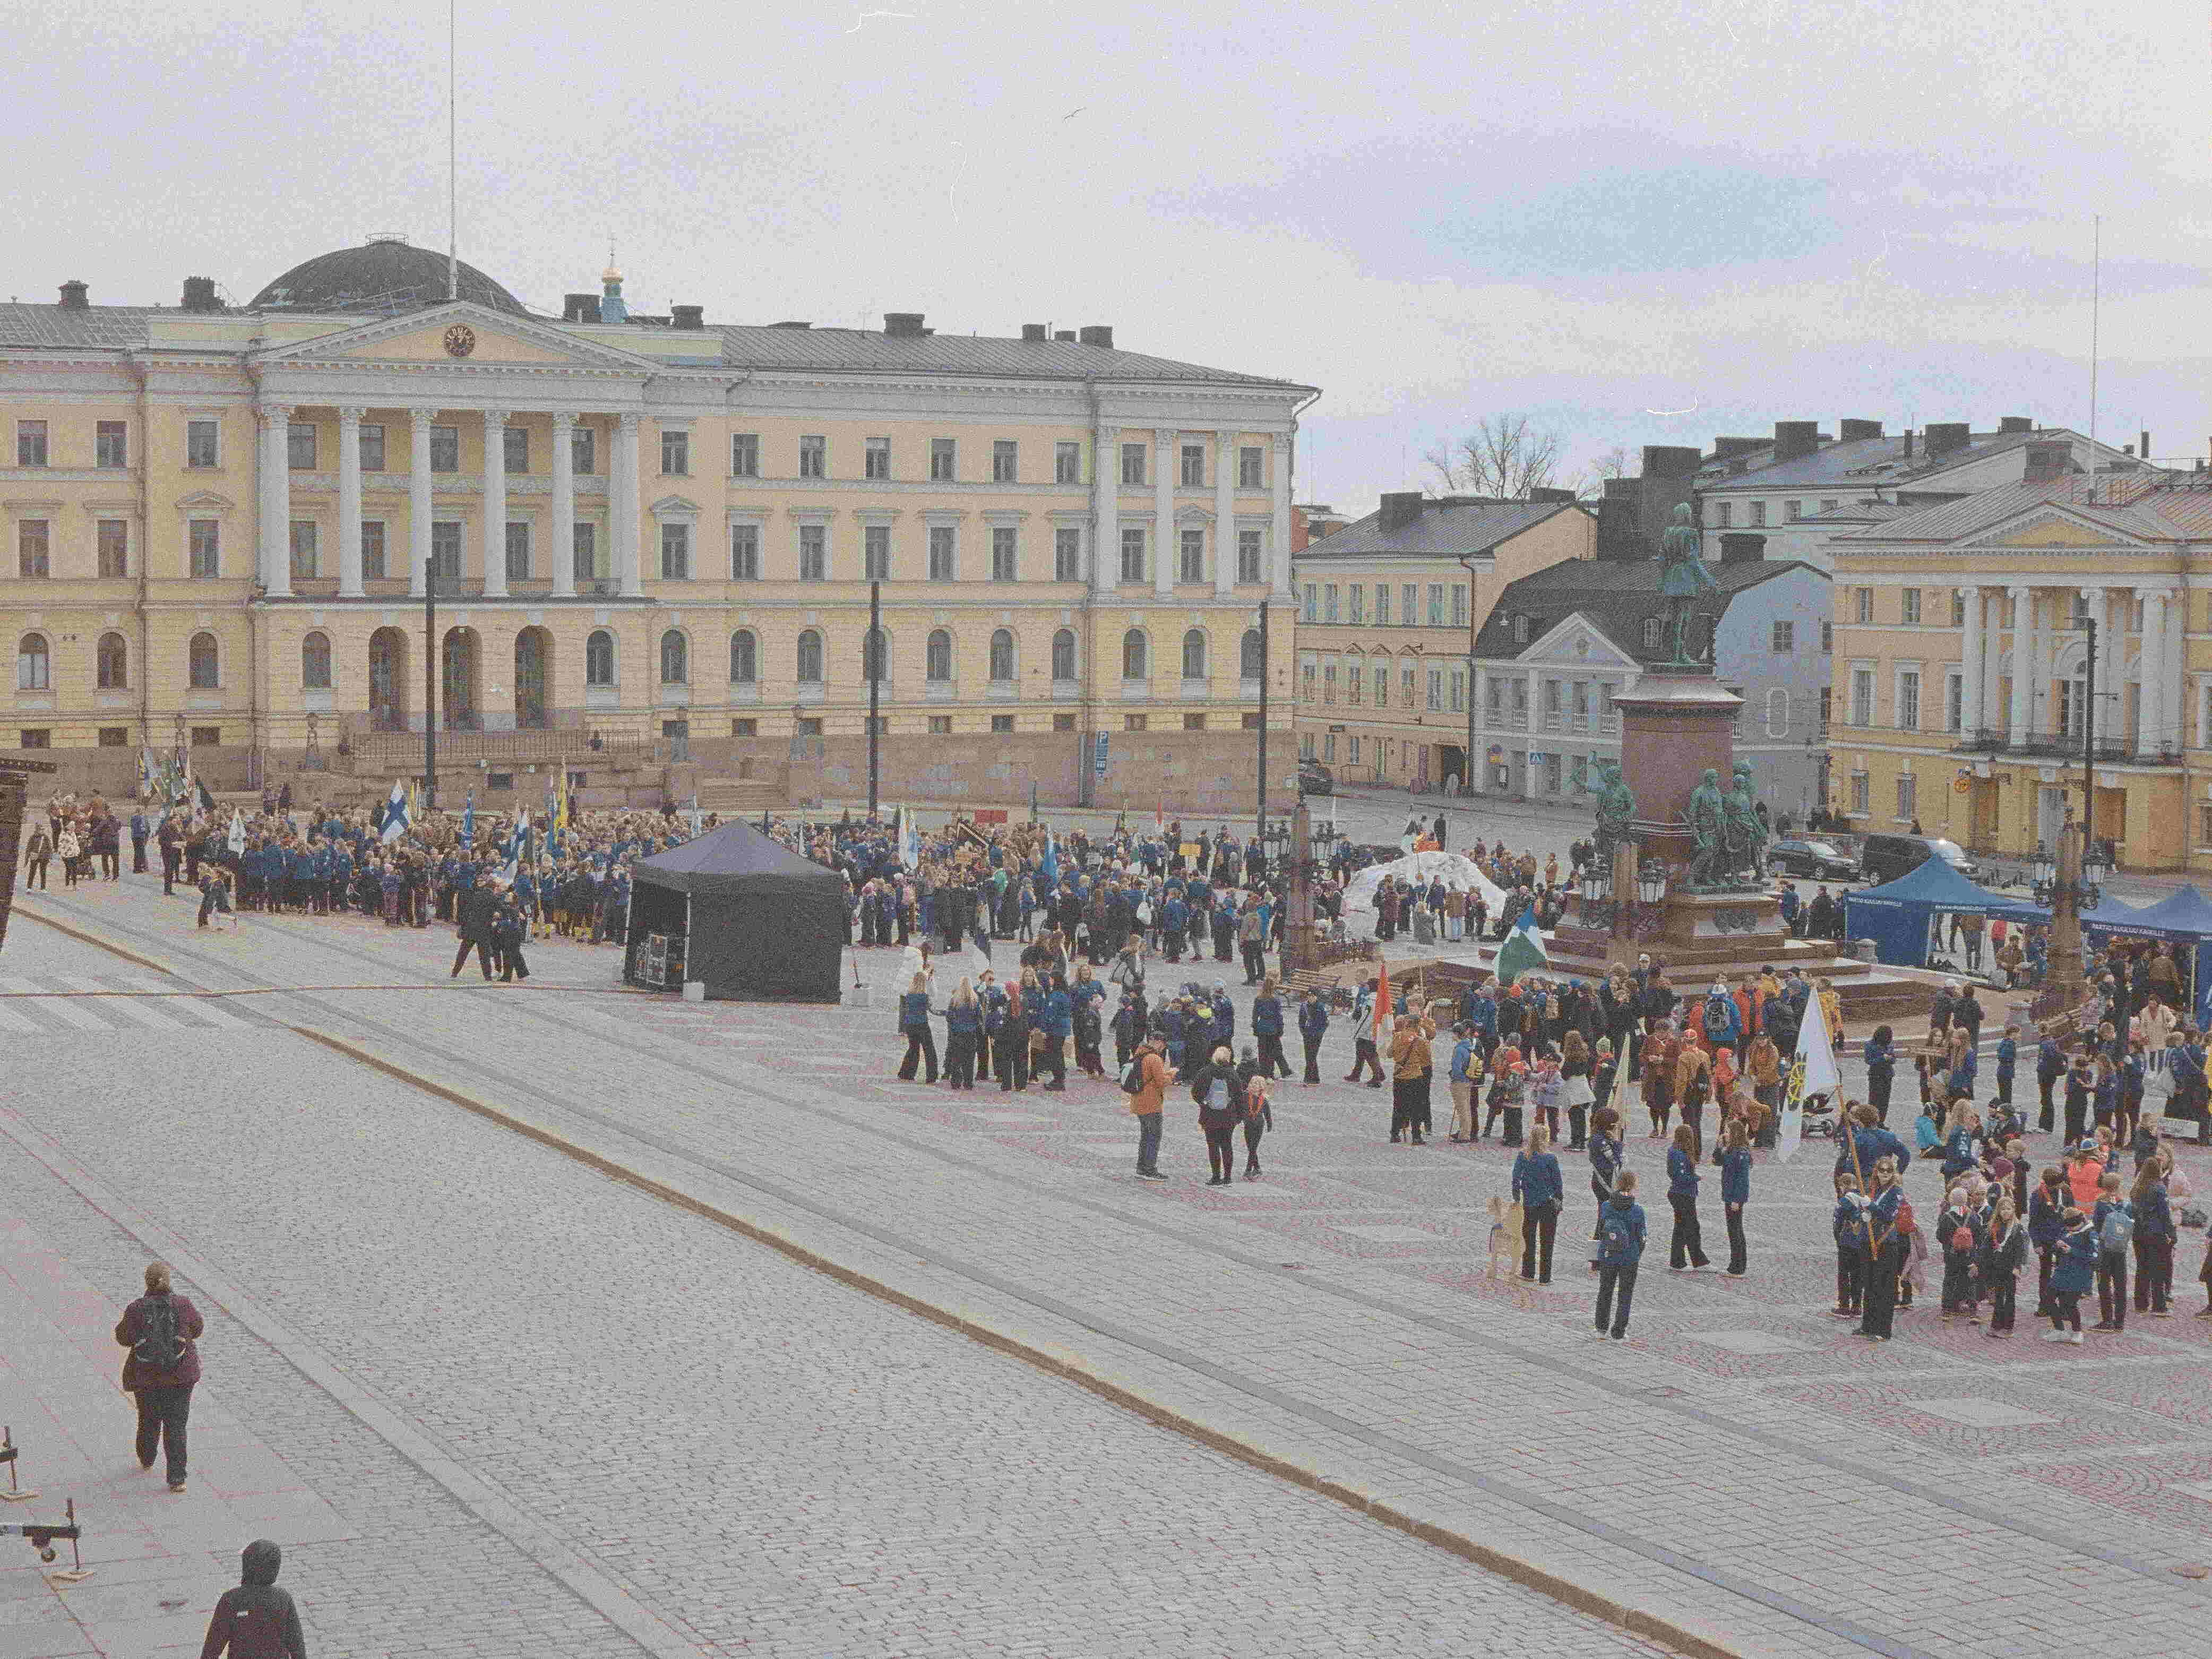
\includegraphics[width=0.9\linewidth]{assets/paraati4}
	\end{center}

	\vspace*{-0.32cm}
	\small Senaatintorilla löytyi yli kaksi tuhatta partiolaista Helsingistä, Espoosta, Vantaasta ja Kauniaisesta. Siellä marsittiin, nautitiin musiikista ja ajoittain auringosta.

	Paraatin päätteeksi, KuRu:n osasto sai vielä maistuva lounas läheisessä \mbox{pitseriassa}!

	\columnbreak

	\begin{center}
		\noindent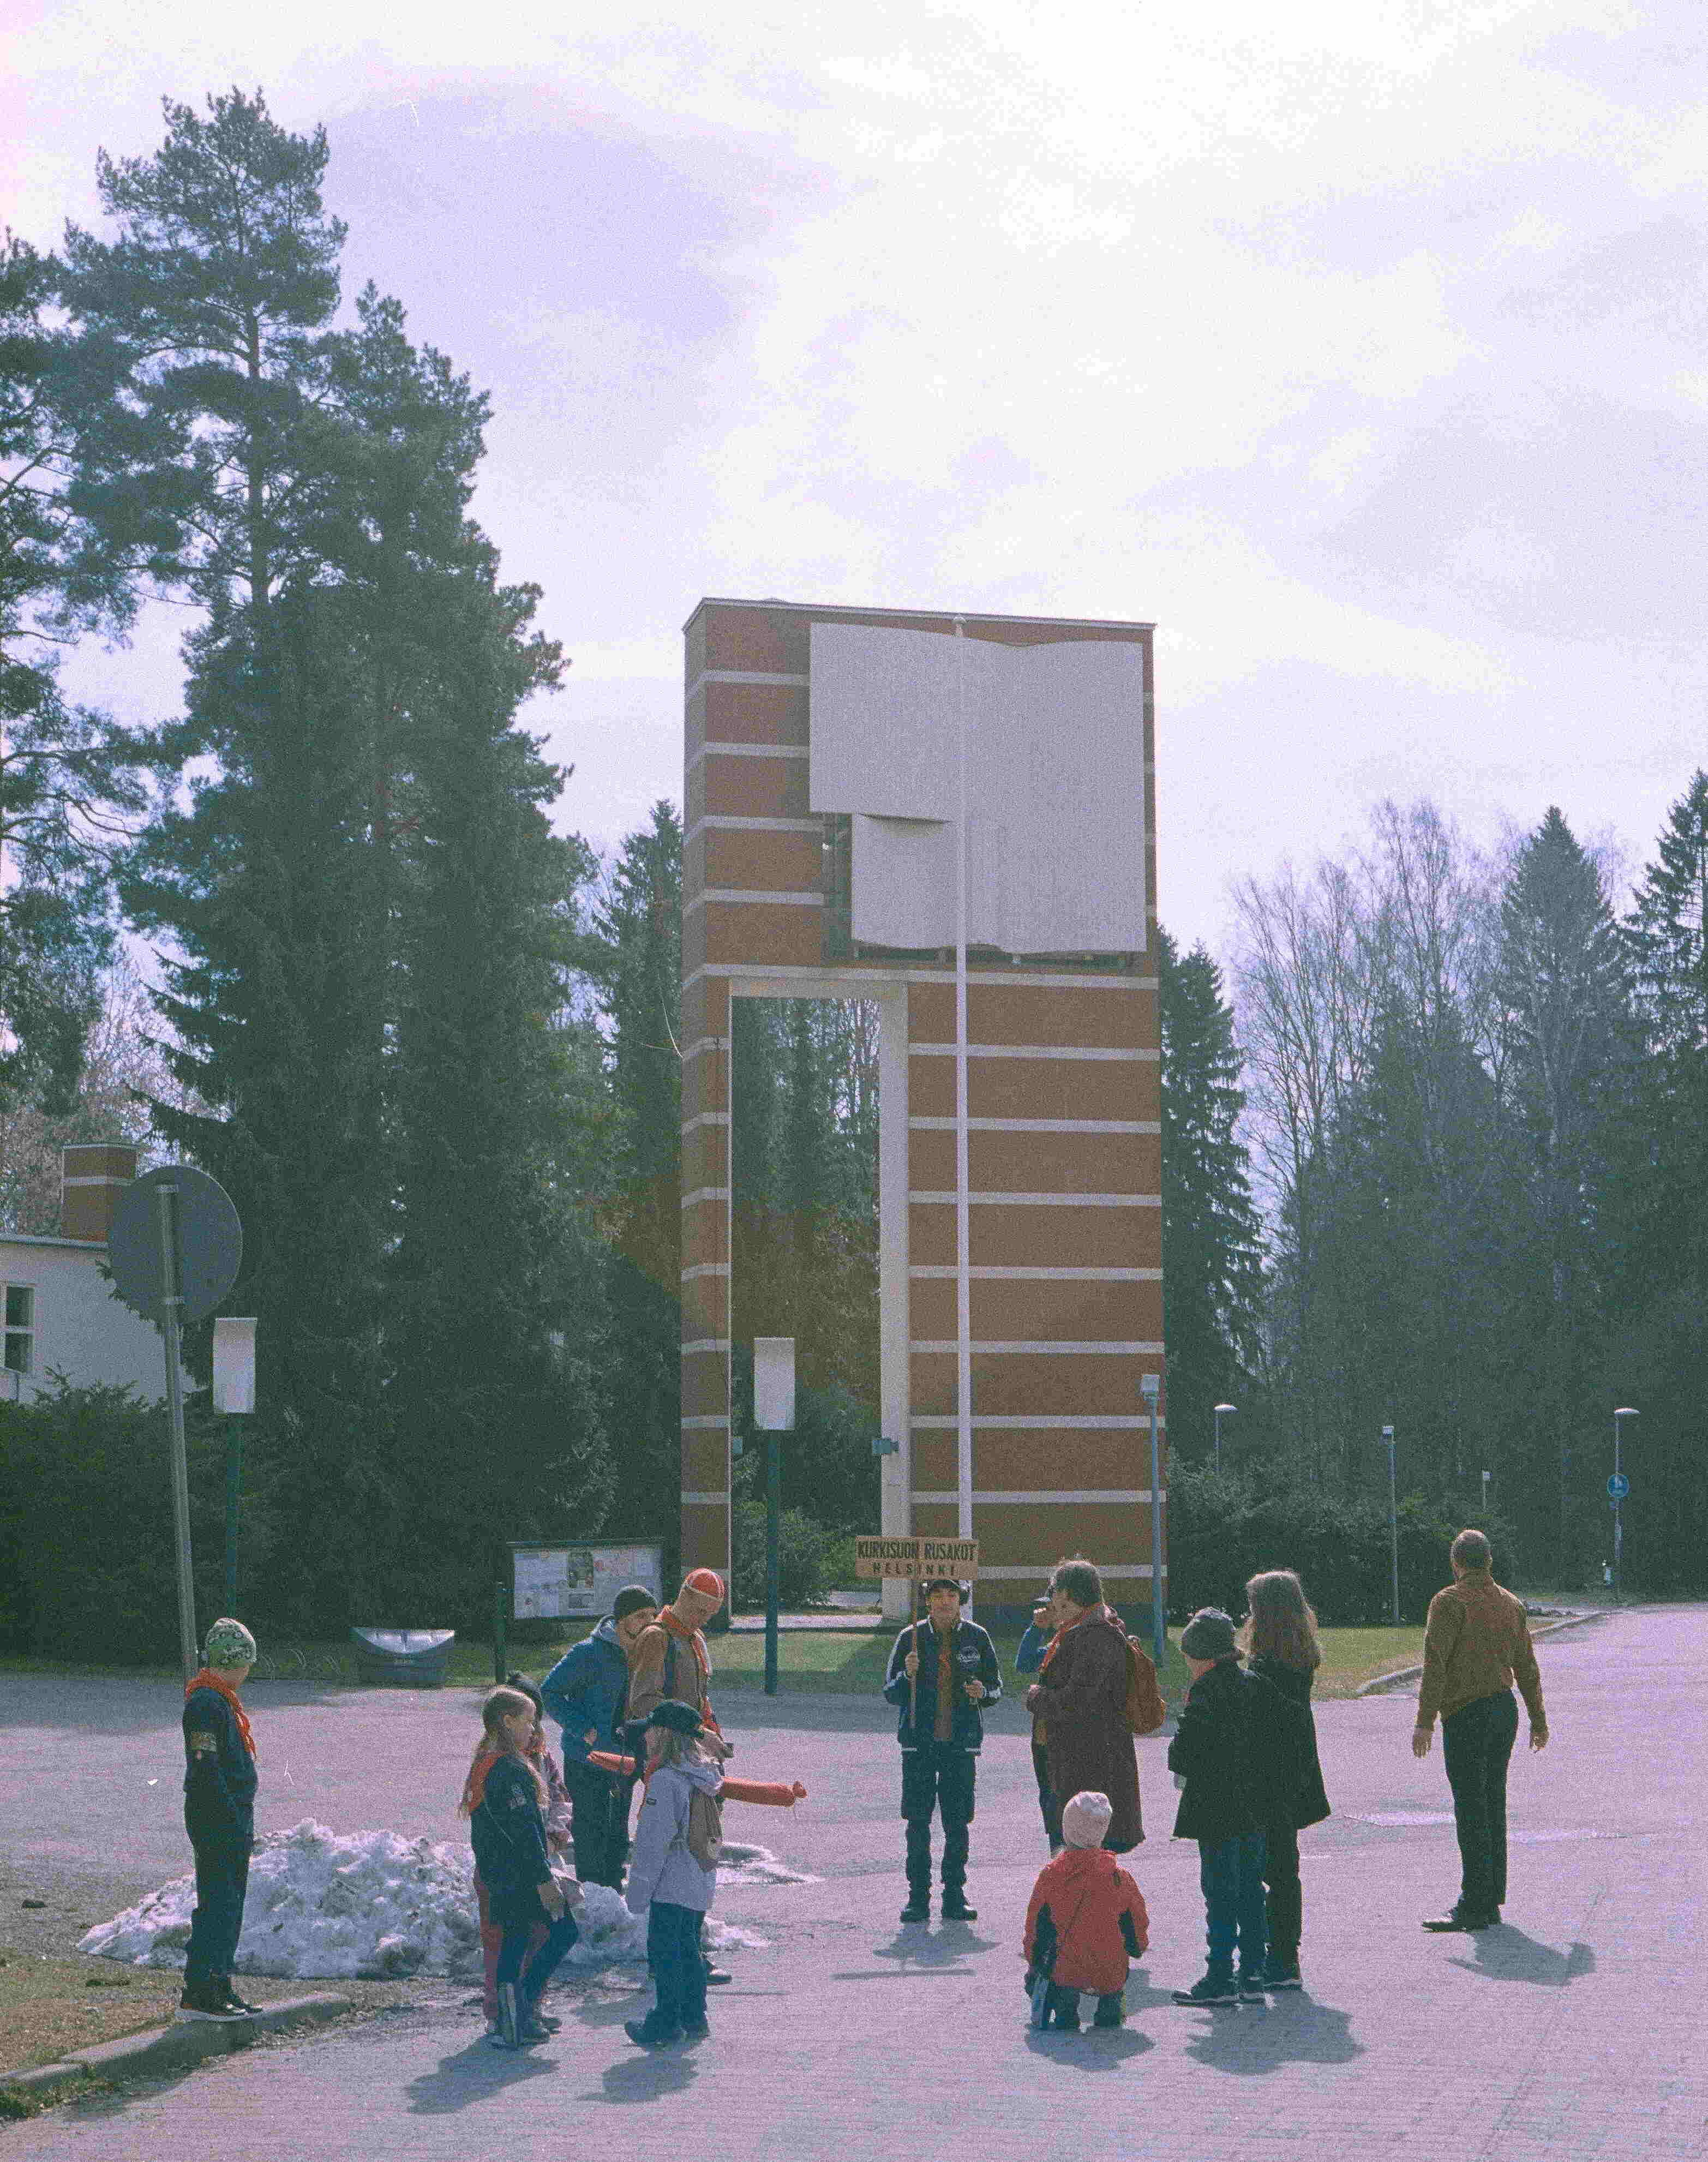
\includegraphics[width=0.9\linewidth]{assets/paraati2}
	\end{center}

	\vspace*{-0.32cm}
	\ldots ja pari päivää myöhemmin, kokoontui keväisessä kelissä ja matkusti kohti keskustan.

	\begin{center}
		\noindent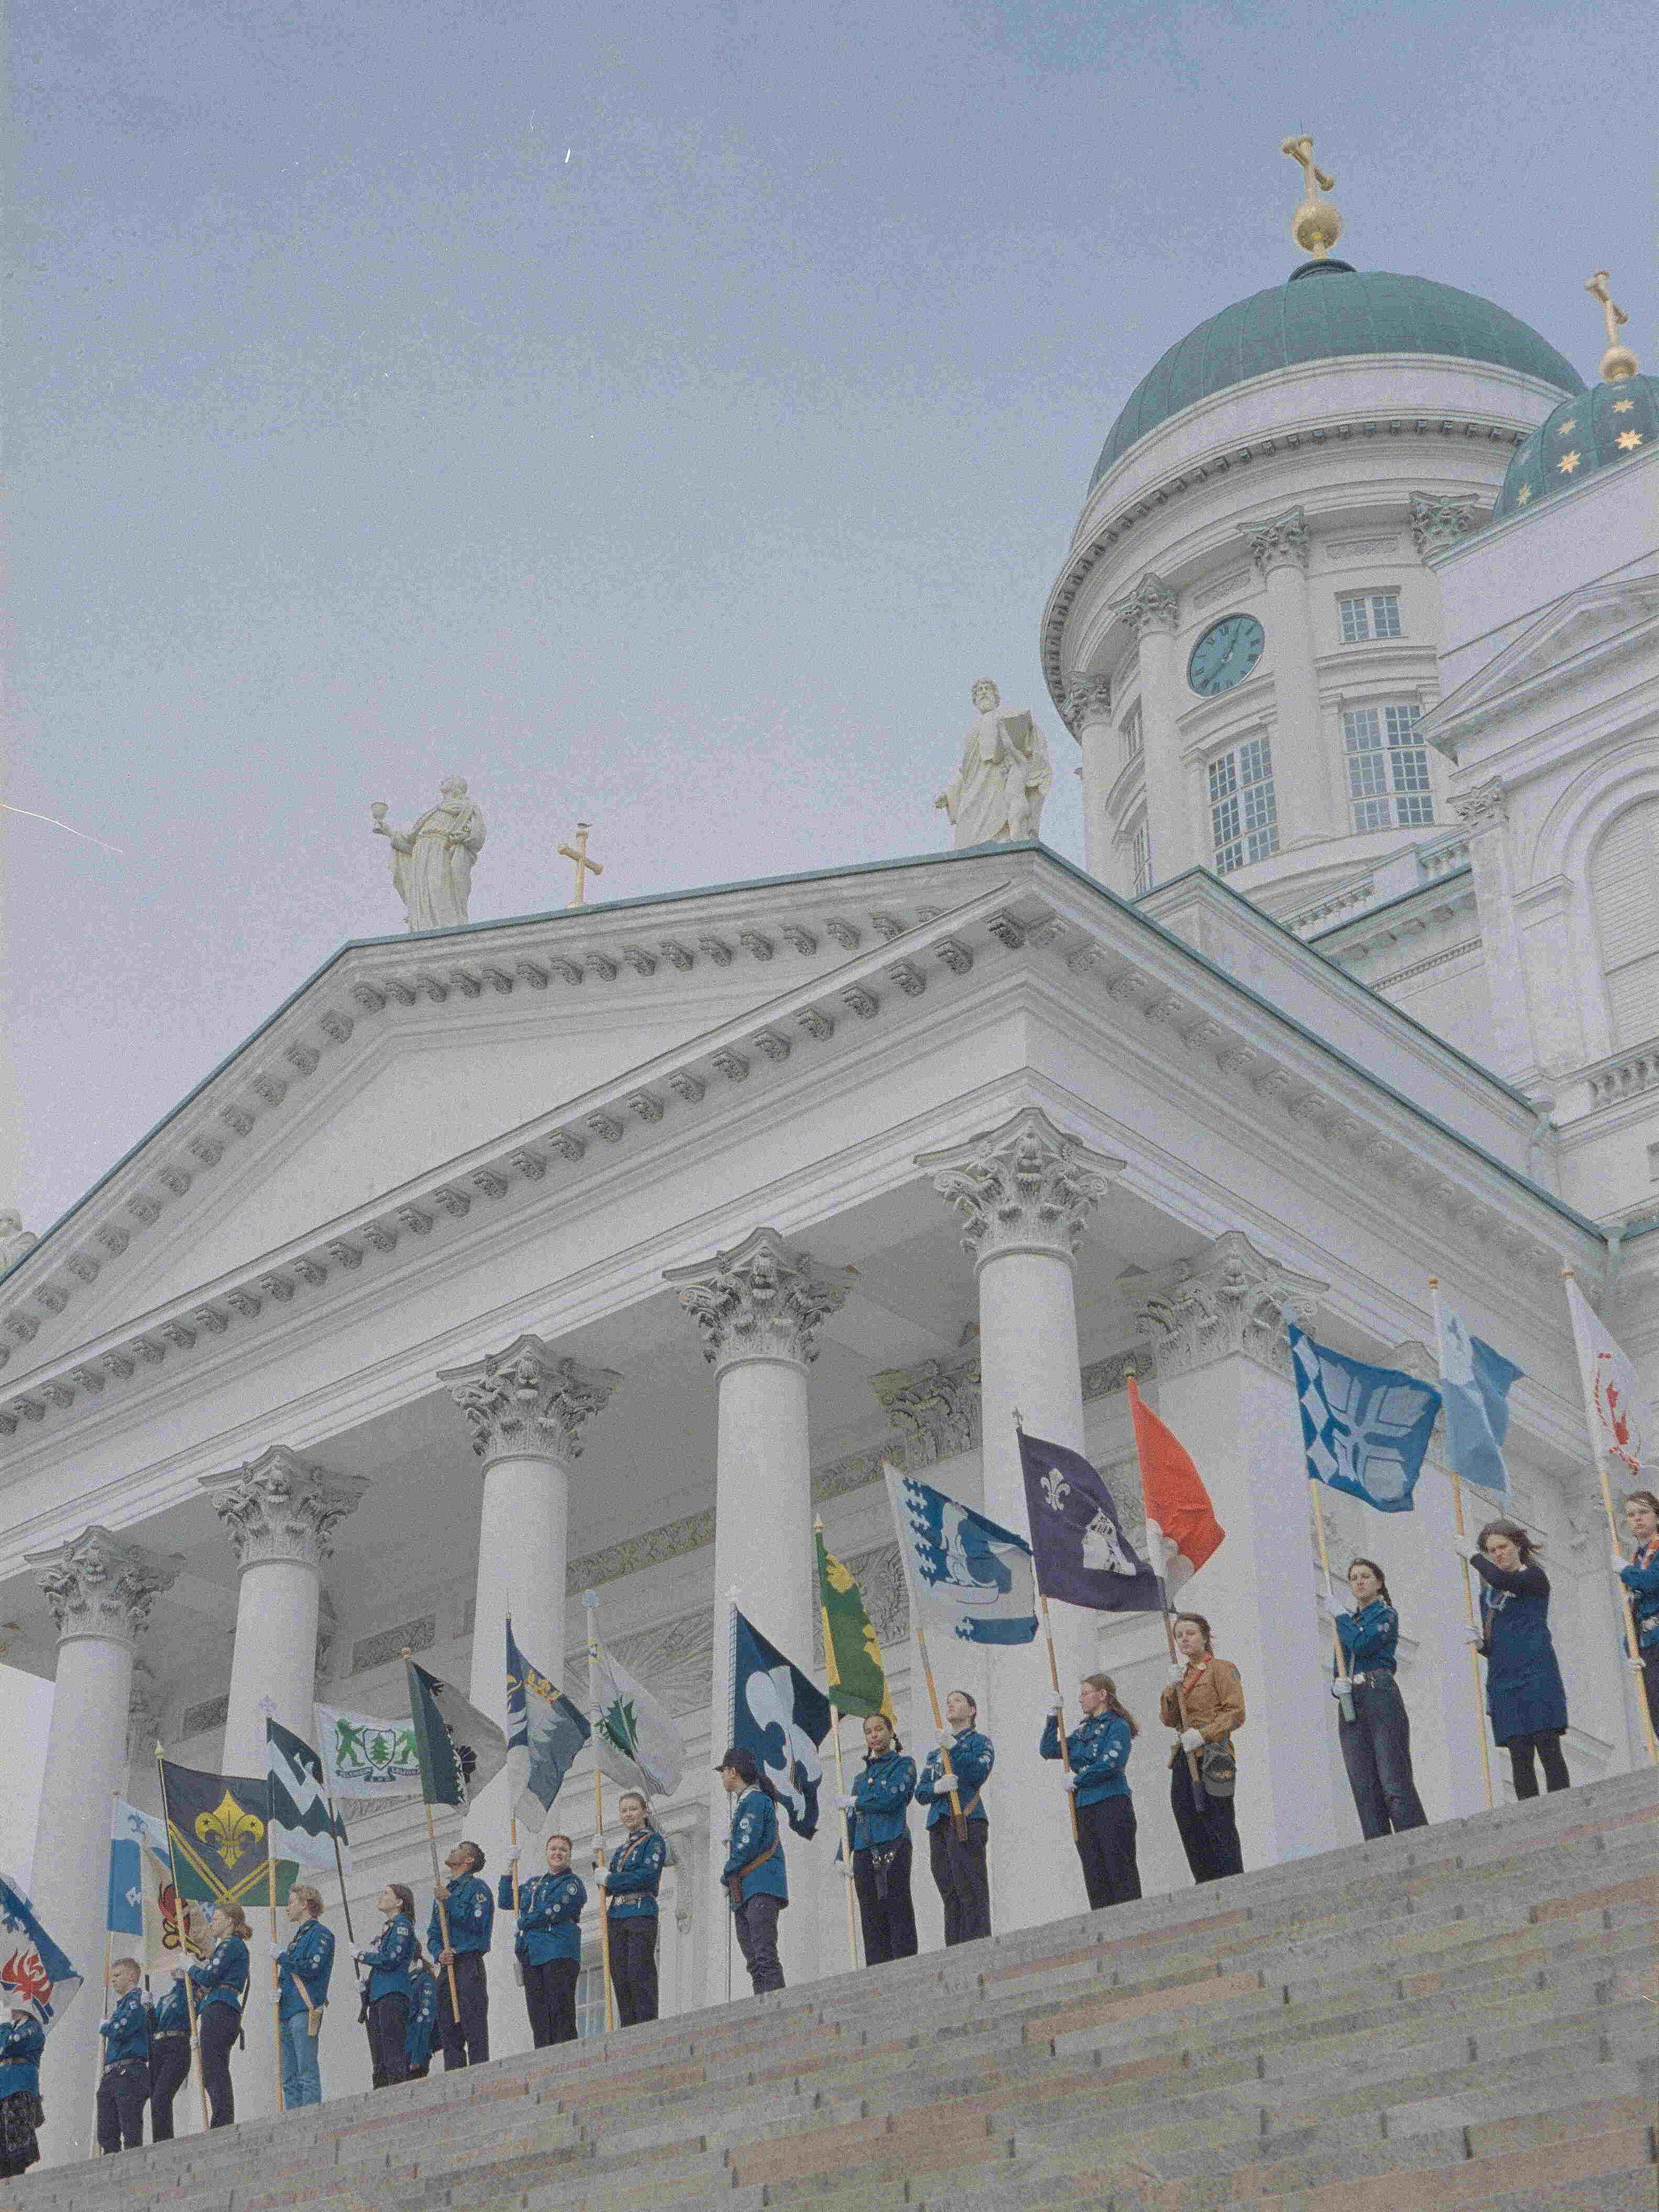
\includegraphics[width=0.9\linewidth]{assets/paraati3}
	\end{center}
	% \vspace*{-2.00cm}


\end{multicols}


\medskip
\noindent\null\hfill Tanguy Gérôme


% \clearpage
% \subsection{Veneen oma retki 3.–5.5.}

\clearpage
\subsection{Pyörävaellus 9.–12.5. KESKEN}

\begin{multicols}{2}


	\begin{center}
		\noindent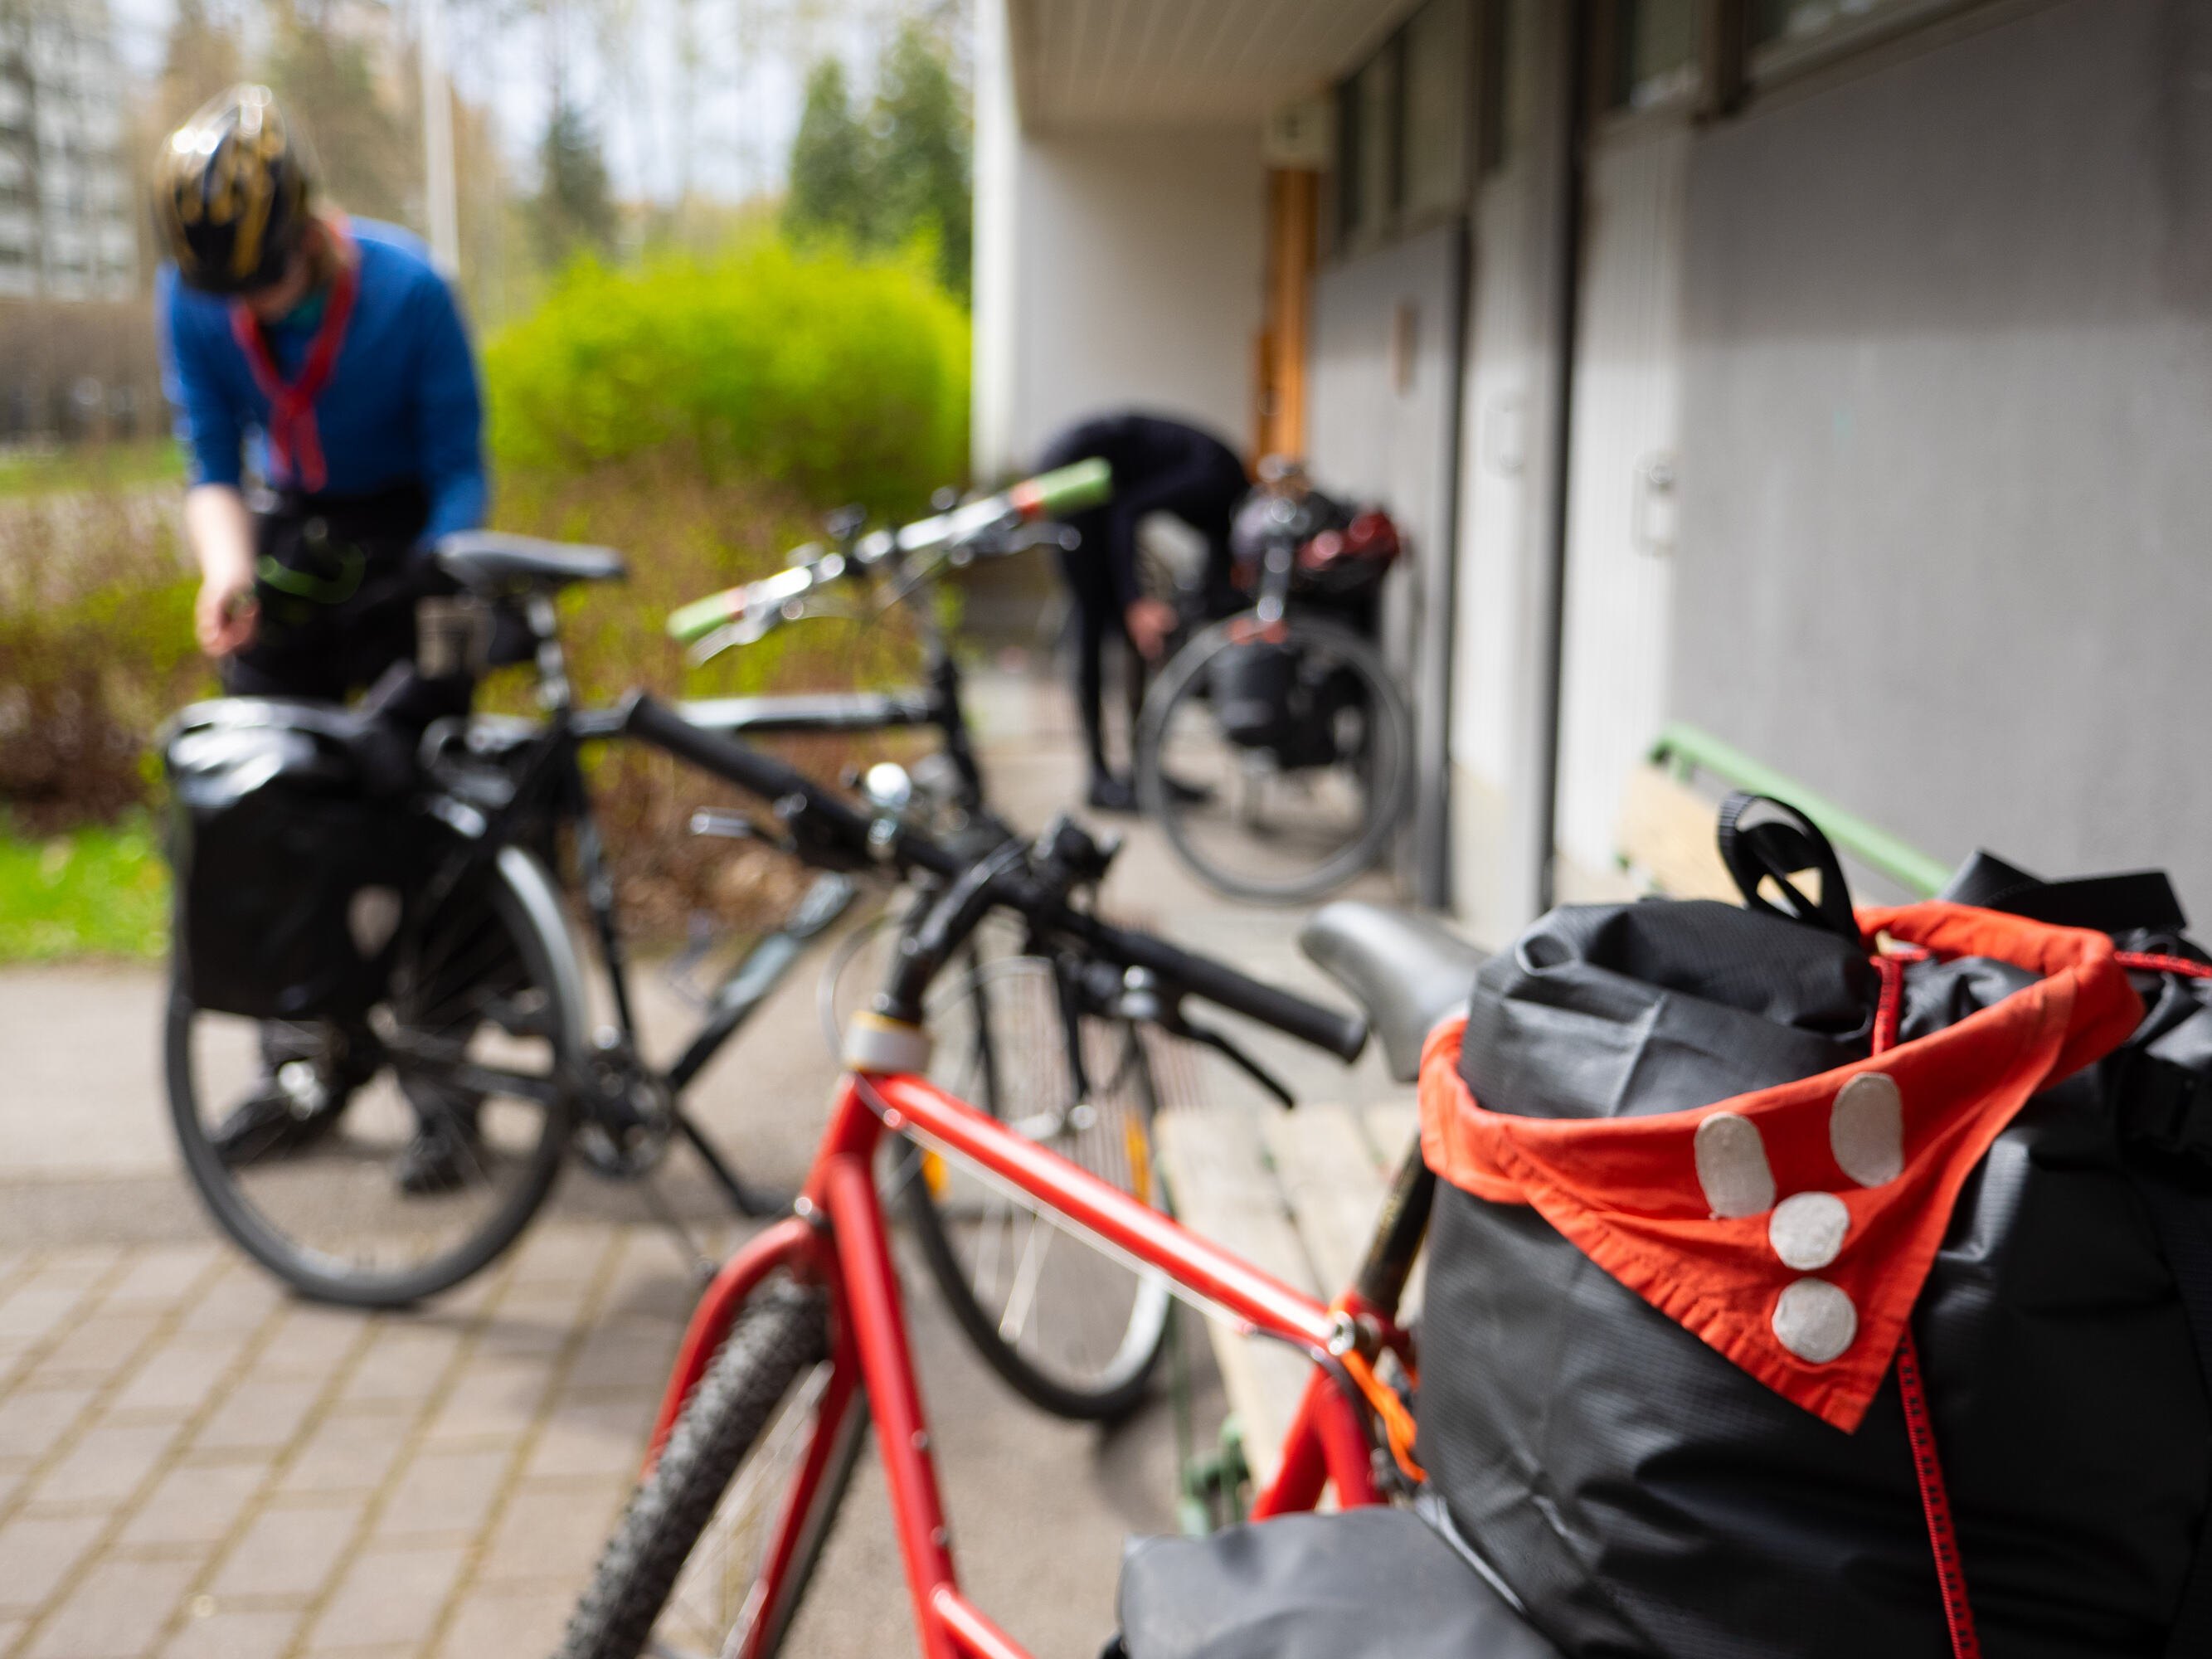
\includegraphics[width=0.94\linewidth]{assets/pyörävaellus1}
		\noindent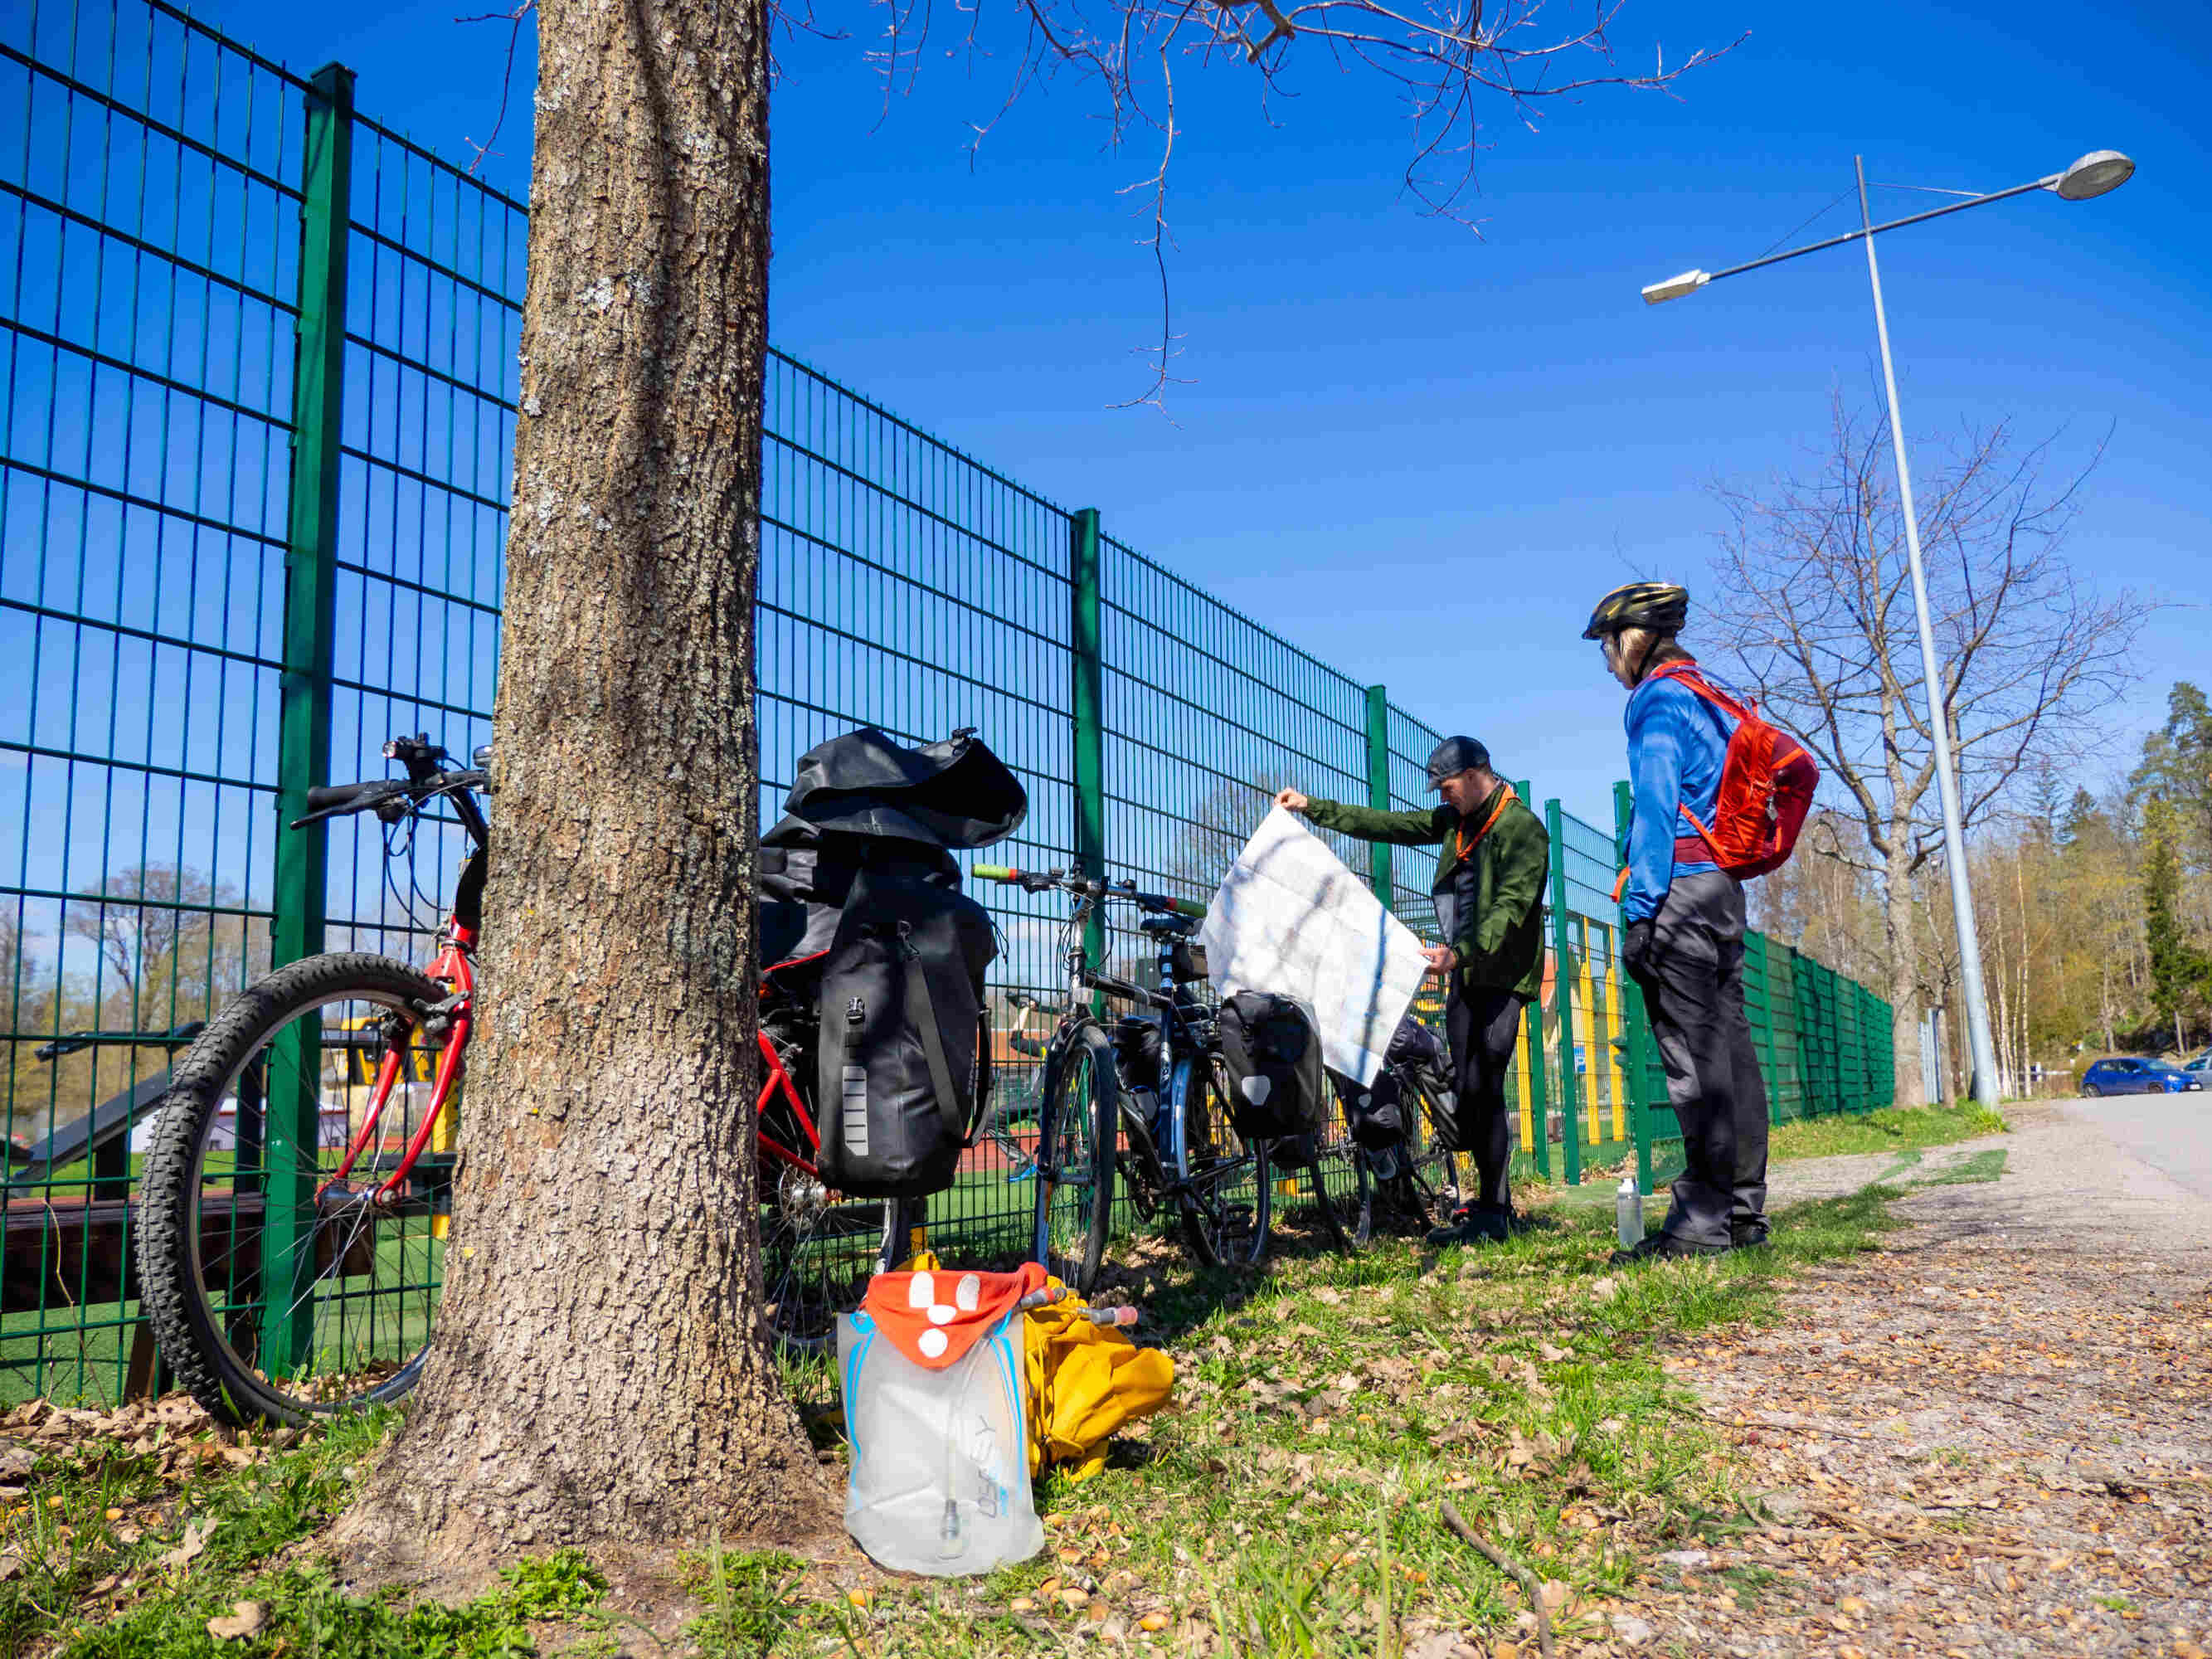
\includegraphics[width=0.94\linewidth]{assets/pyörävaellus3}
		\noindent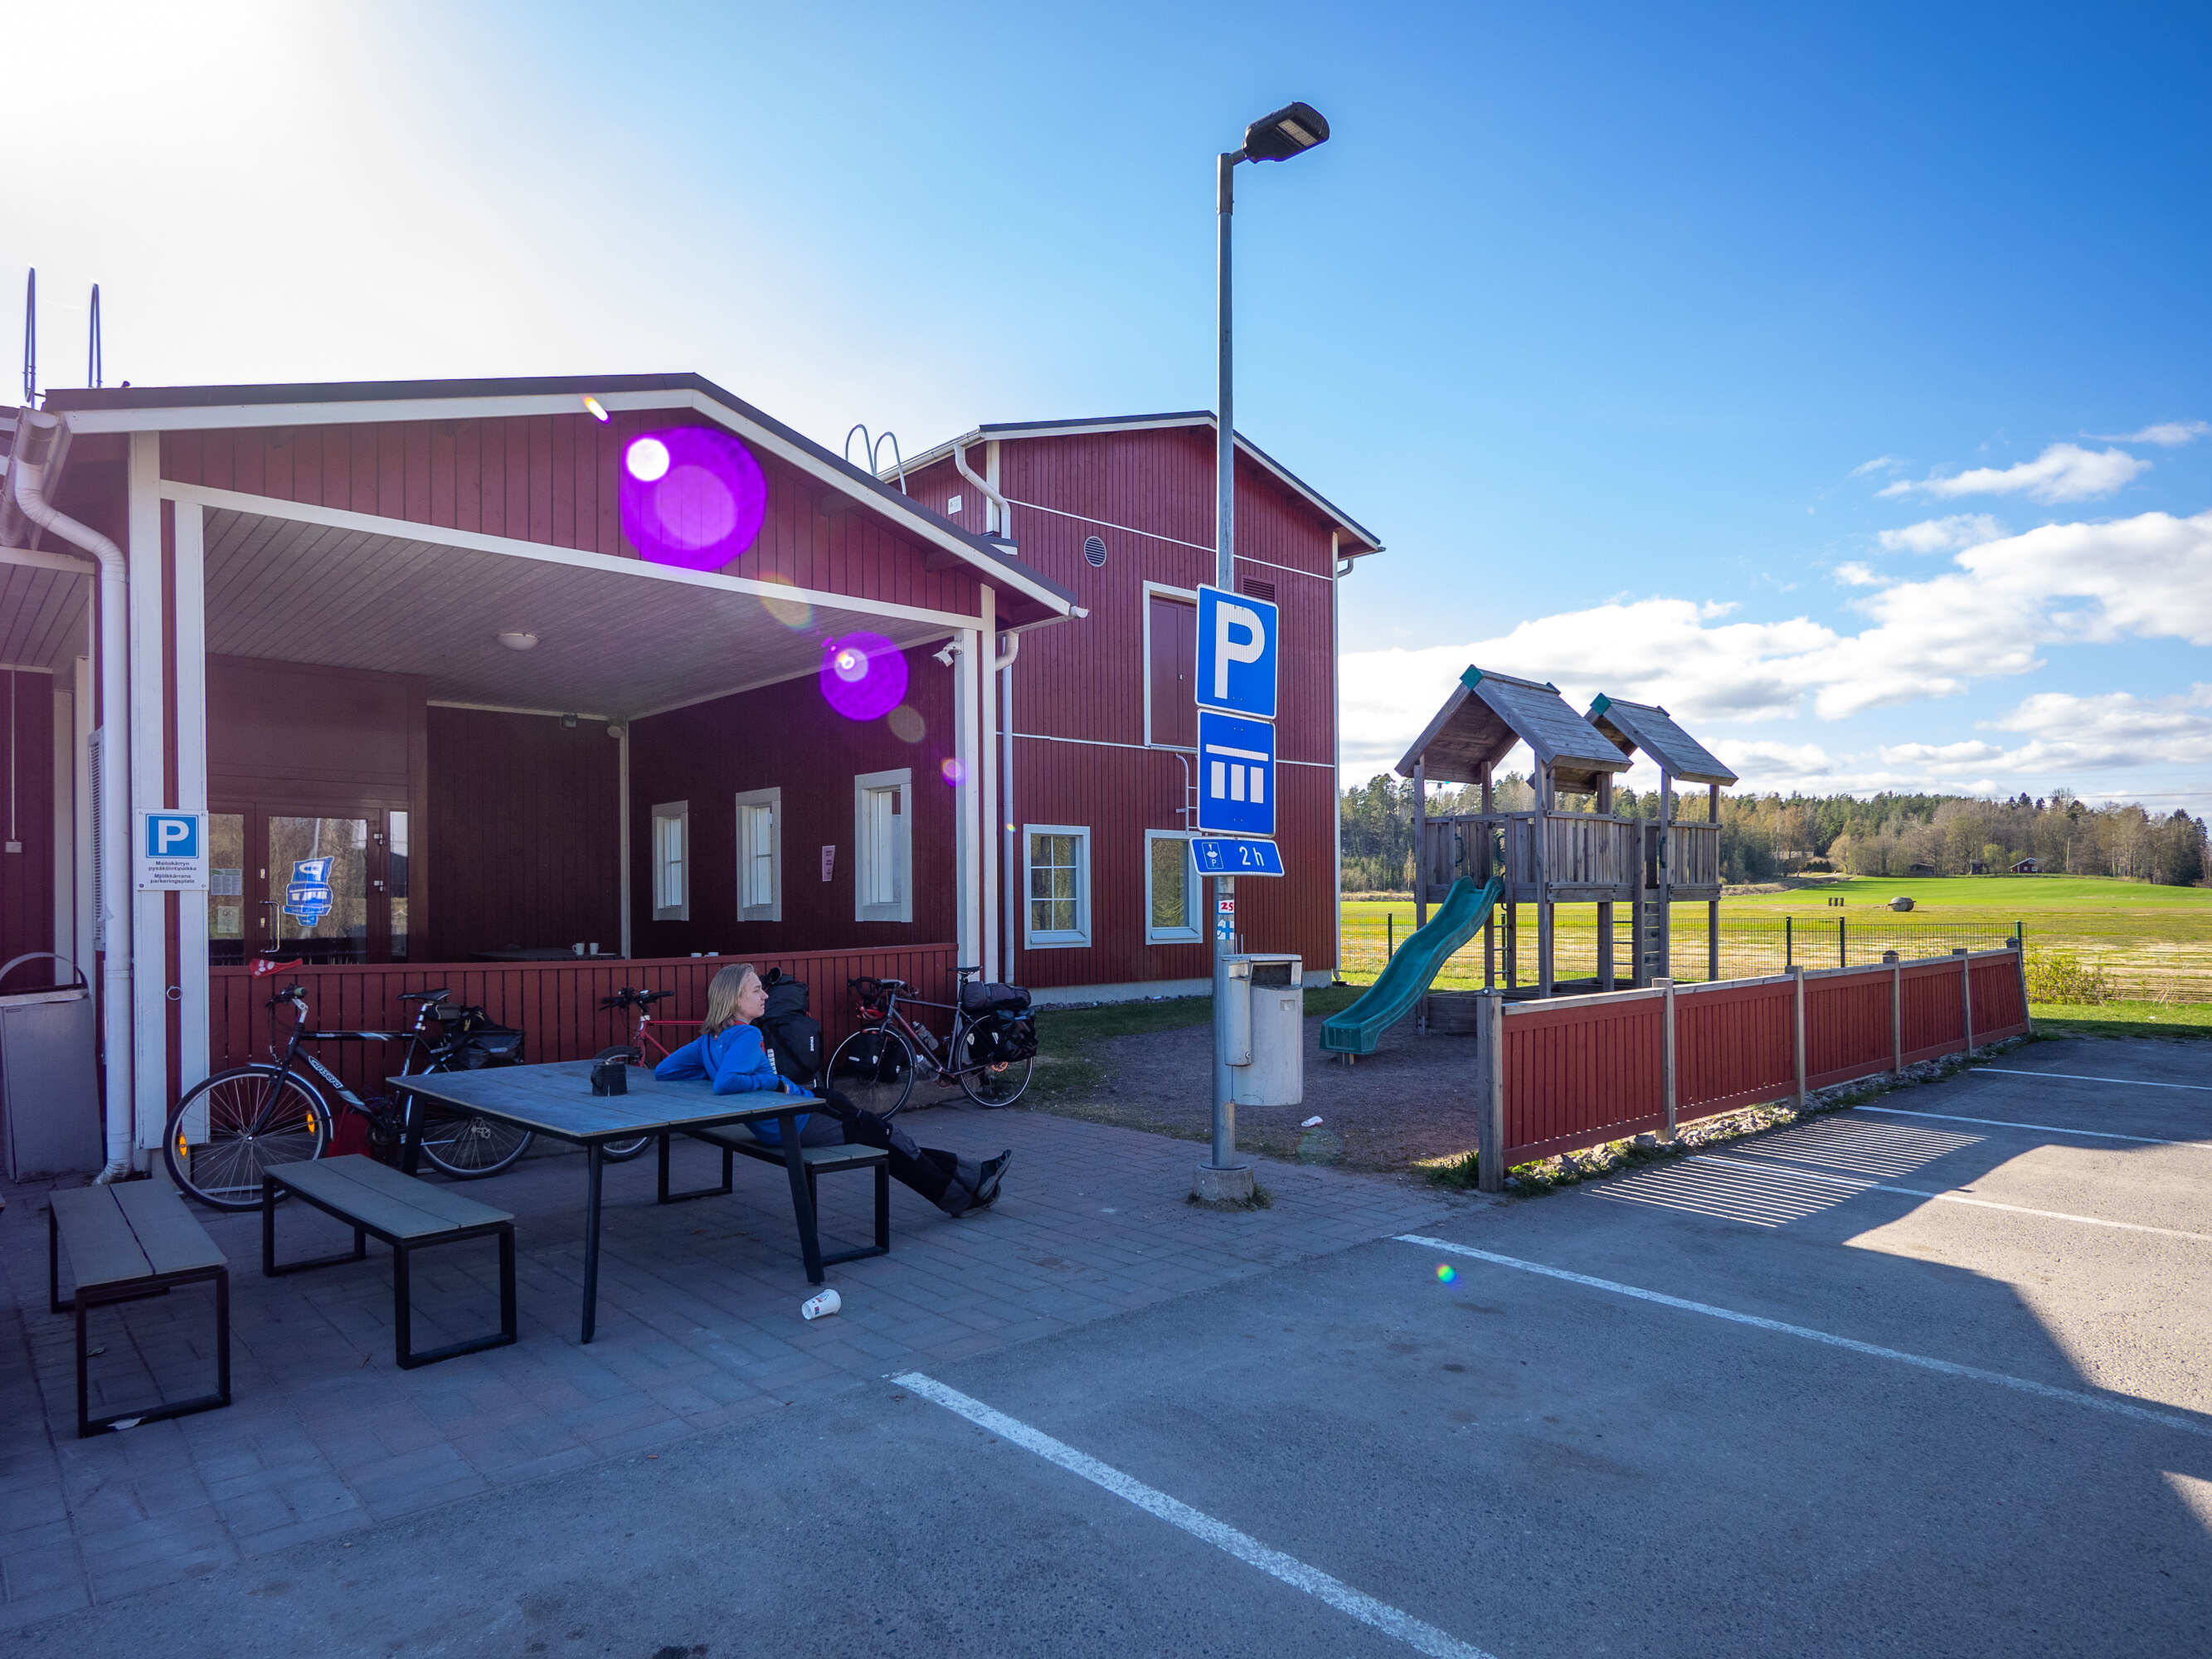
\includegraphics[width=0.94\linewidth]{assets/pyörävaellus4}
		\noindent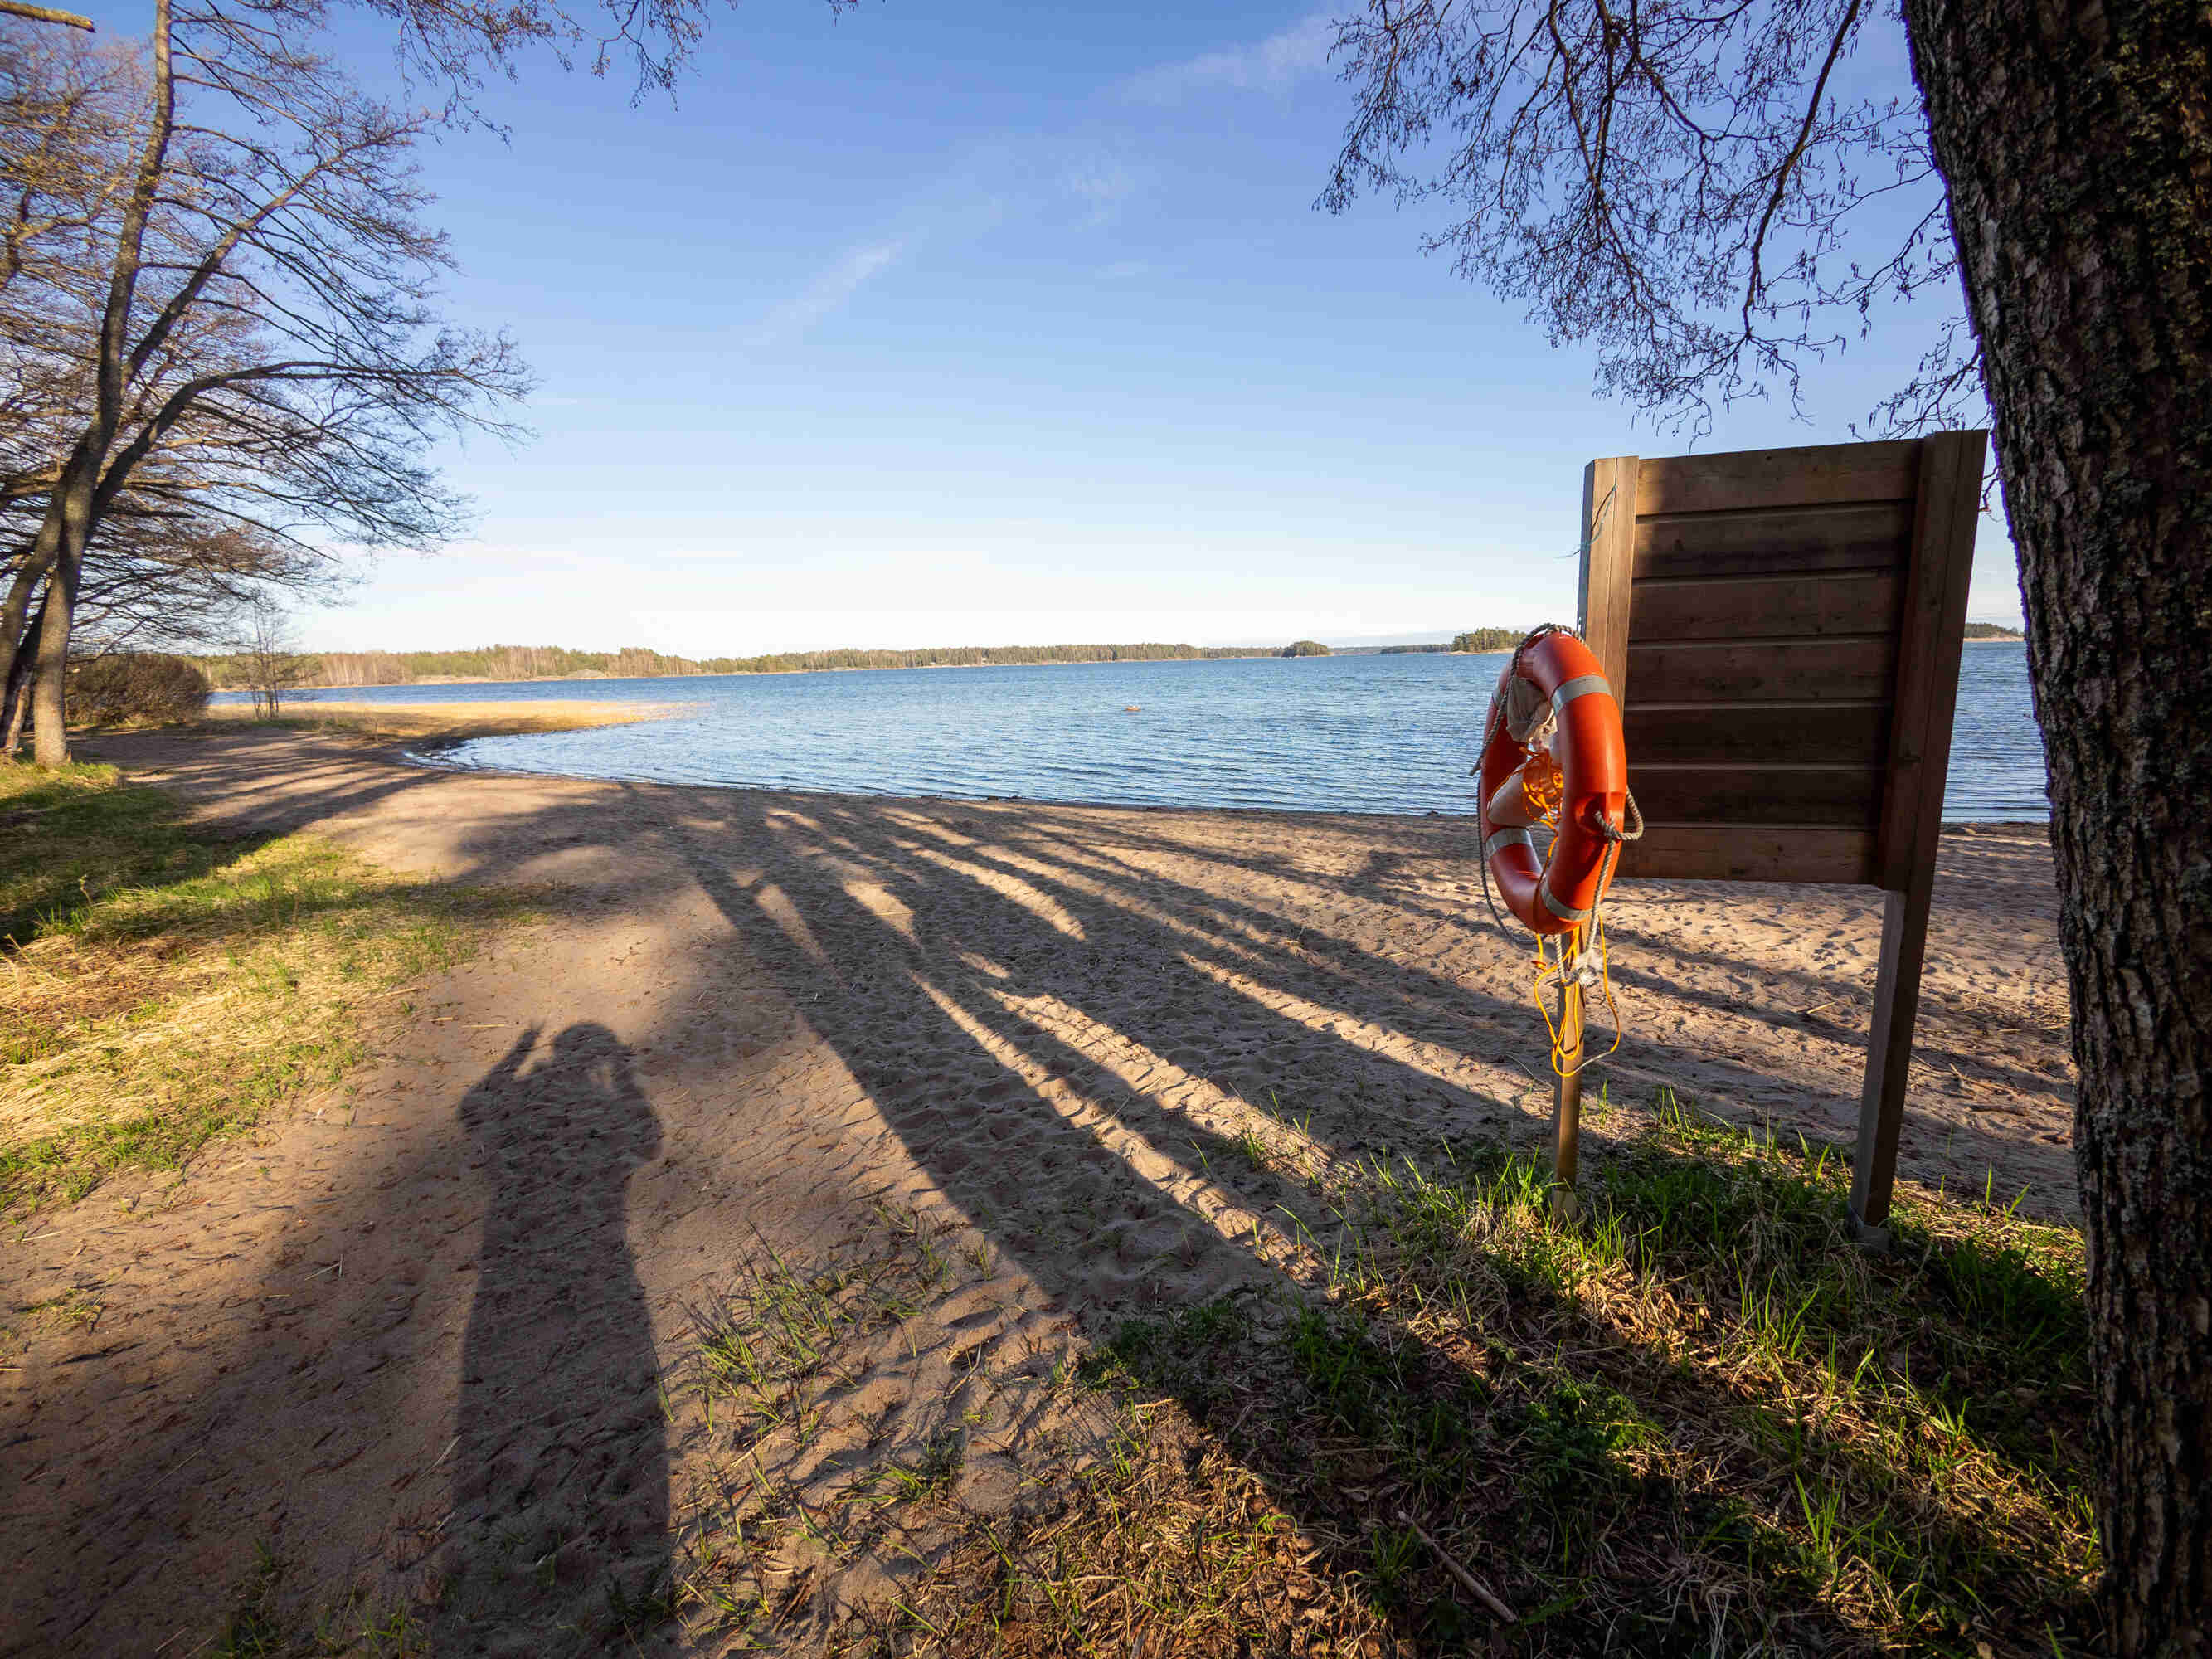
\includegraphics[width=0.94\linewidth]{assets/pyörävaellus5}
	\end{center}

	\columnbreak

	% \small
	Kolme rusakkoa lähtivät pyöräilemään KuRu:n varastolta torstaina
	9.5. aamuna, lännen kohti. Matka alkoi pilvisessä ja viileässä säässä,
	mutta kuten rusakot toivoivat sade jäi pois, ja aurinko saapui pian.

	Ensimmäinen tekninen vika ilmestyi jo 600 metrin jälkeen, ja nopeasti
	korjaantui. Rusakot pyöräilivat Kehä 1:n kautta Espooseen, ja
	ensimmäisen evästauon pidettiin Leppävaarassa. Matka jatkui Turuntien
	kautta, Kauniaisen ohi, Bemböleen. Vielä oli liian aikaisin syömään
	lounas, eli matka jatkui Klauklahteen, jossa valittiin urheilukenttä
	lounaspaikaksi.

	Lounaan jälkeen jatkui matka \mbox{Kirkkonummen} kautta, ja päätimme yöpyä
	meren äärellä, vaikka matka pitenisikin sen vuoksi.
	Ensimmäisen jäätelön syötiin Pickalan huoltoasemalla.

	Jäätelon jälkeen, pieni mutta stressaava Inkoon Rannikkotien pätkä
	odotti meitä, jota seurasi rennompi mutta kuoppainen hiekkatie, ja
	vihdoin löytyi meidän yöpymispaikka: Kopparnäs, Inkoo

	74km jälkeen jotkut rusakoista alkoivat tuntea \textbf{vähän} kipua ja
	\textbf{vähän} väsymystä. Äänekkäät kalatiirat rannalla uhkasivat olla
	antamatta meidän nukkua, mutta onneksi lähtivät illallisen jälkeen.

	\columnbreak

	Sade saapui yöllä, ja kiltisti lähti ennen rusakoiden herätys.

	\columnbreak

	\begin{center}
		\noindent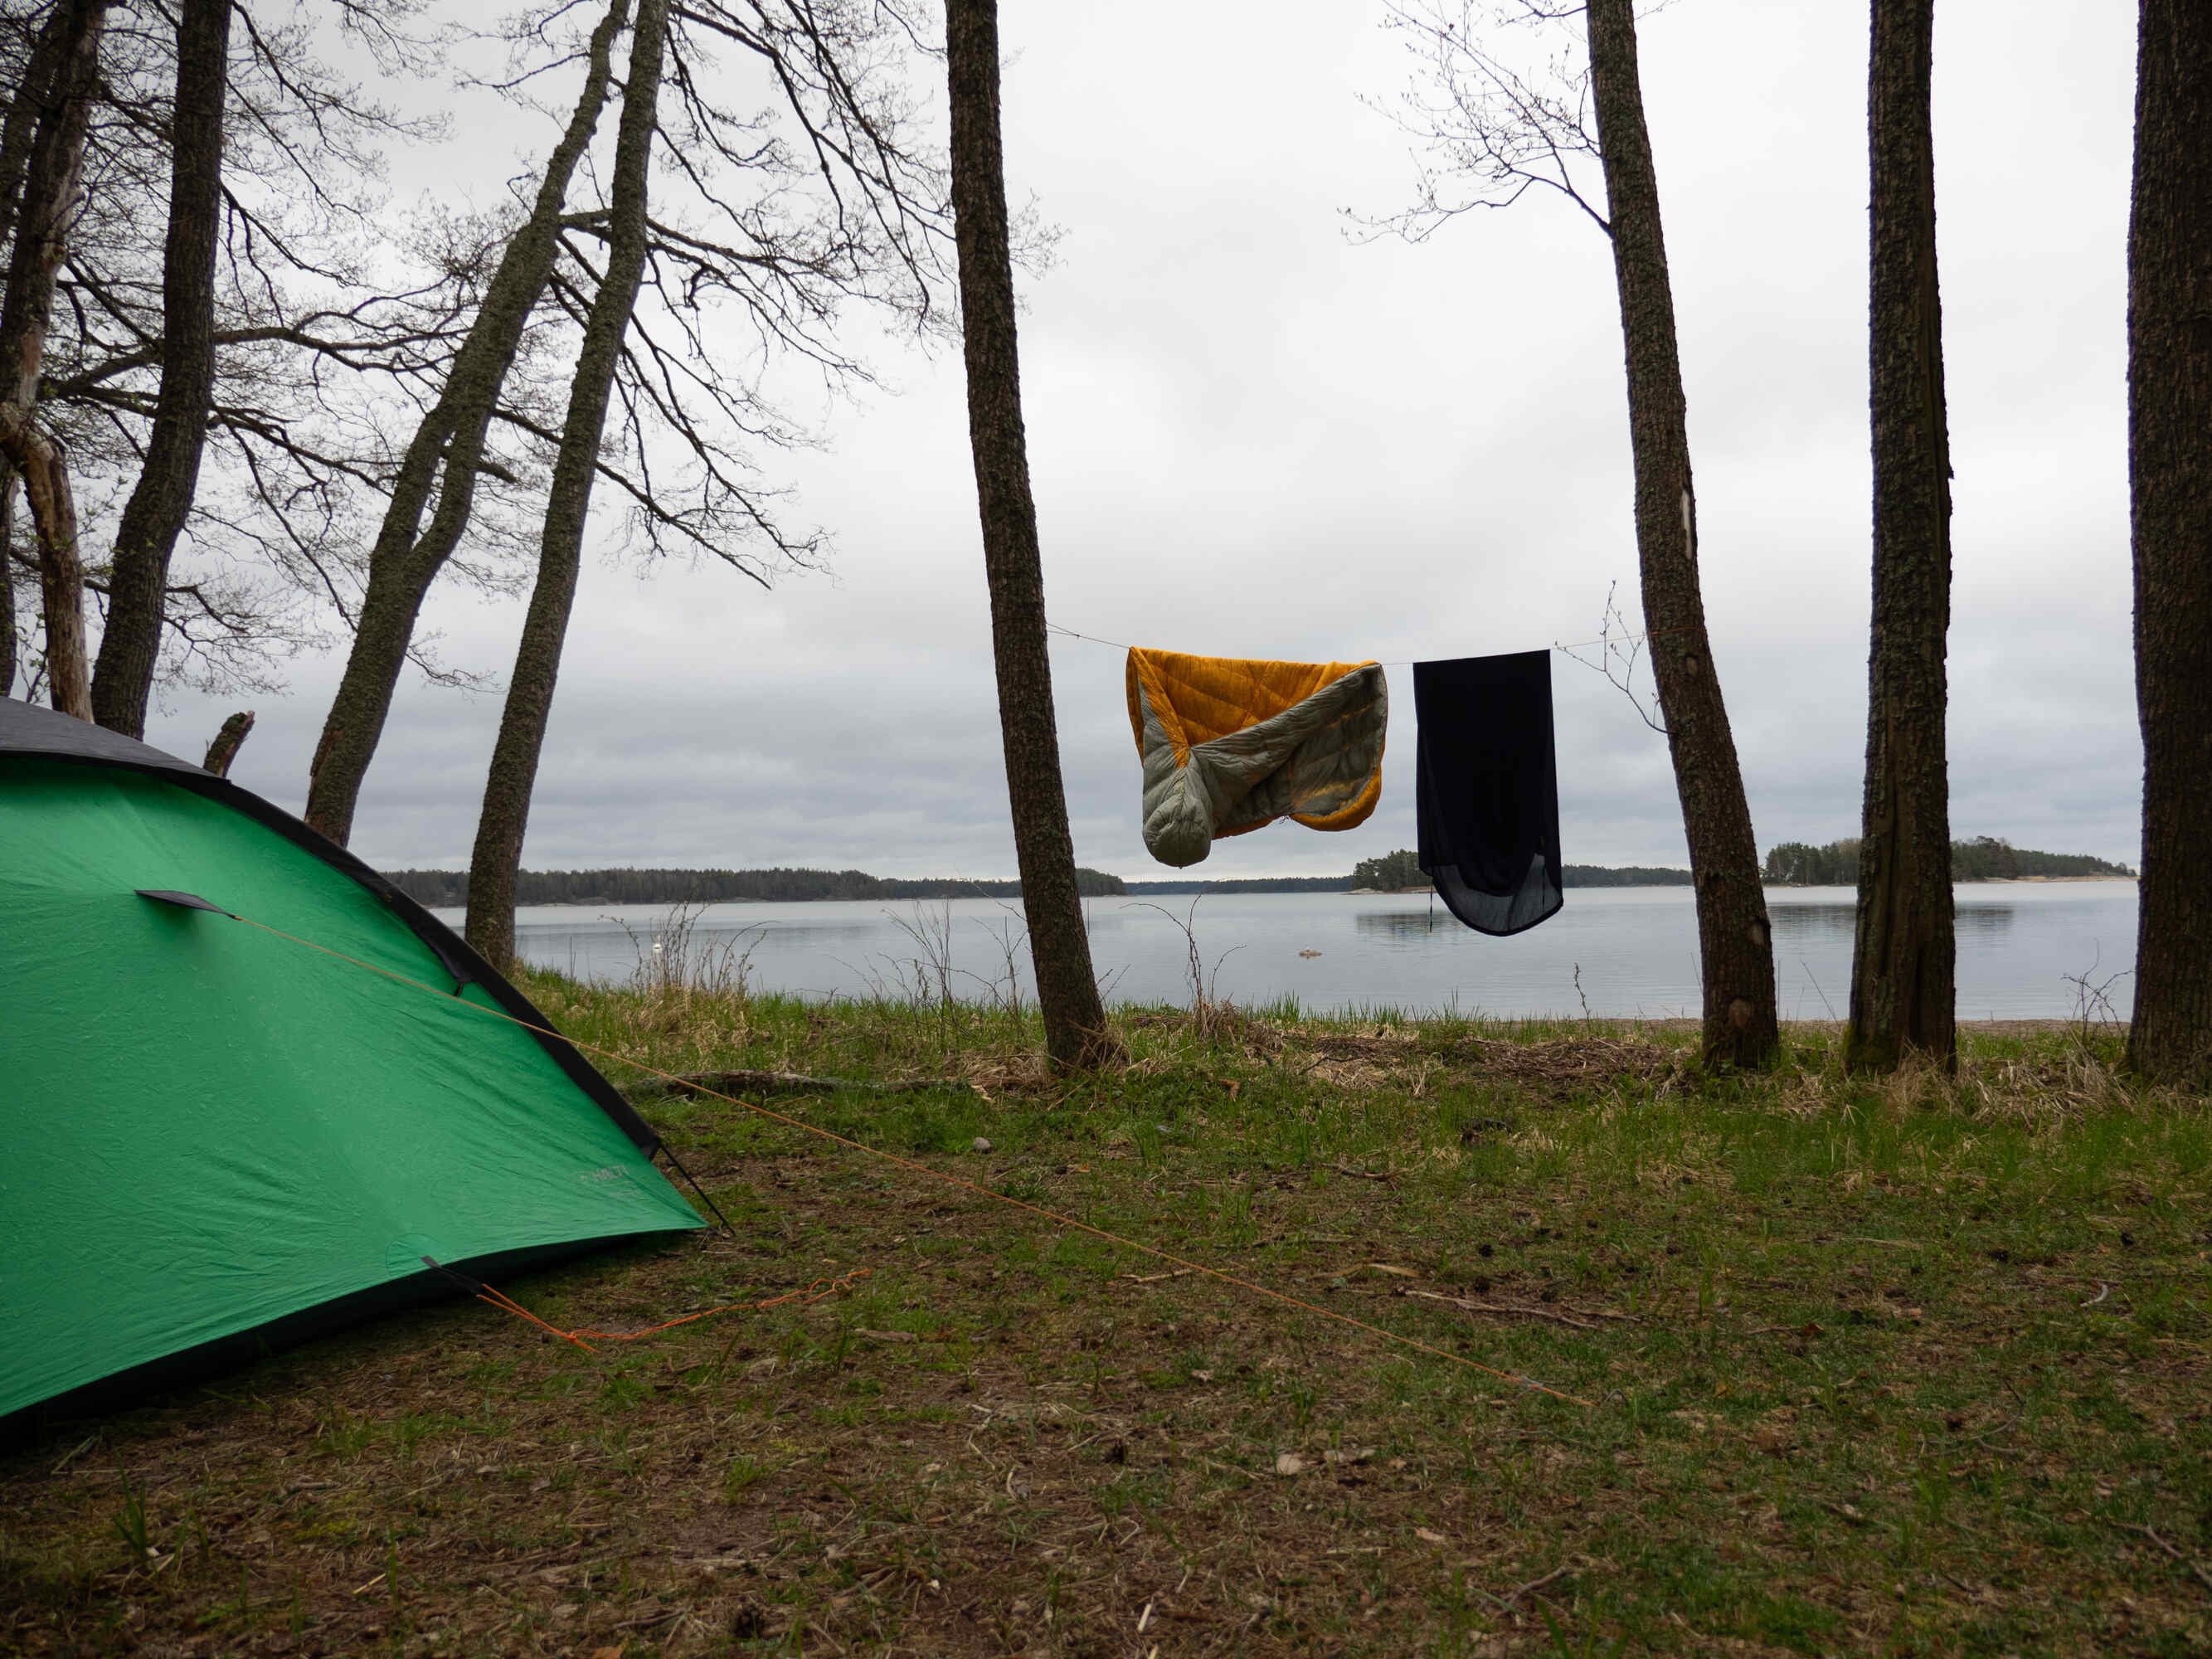
\includegraphics[width=0.94\linewidth]{assets/pyörävaellus6}
		\noindent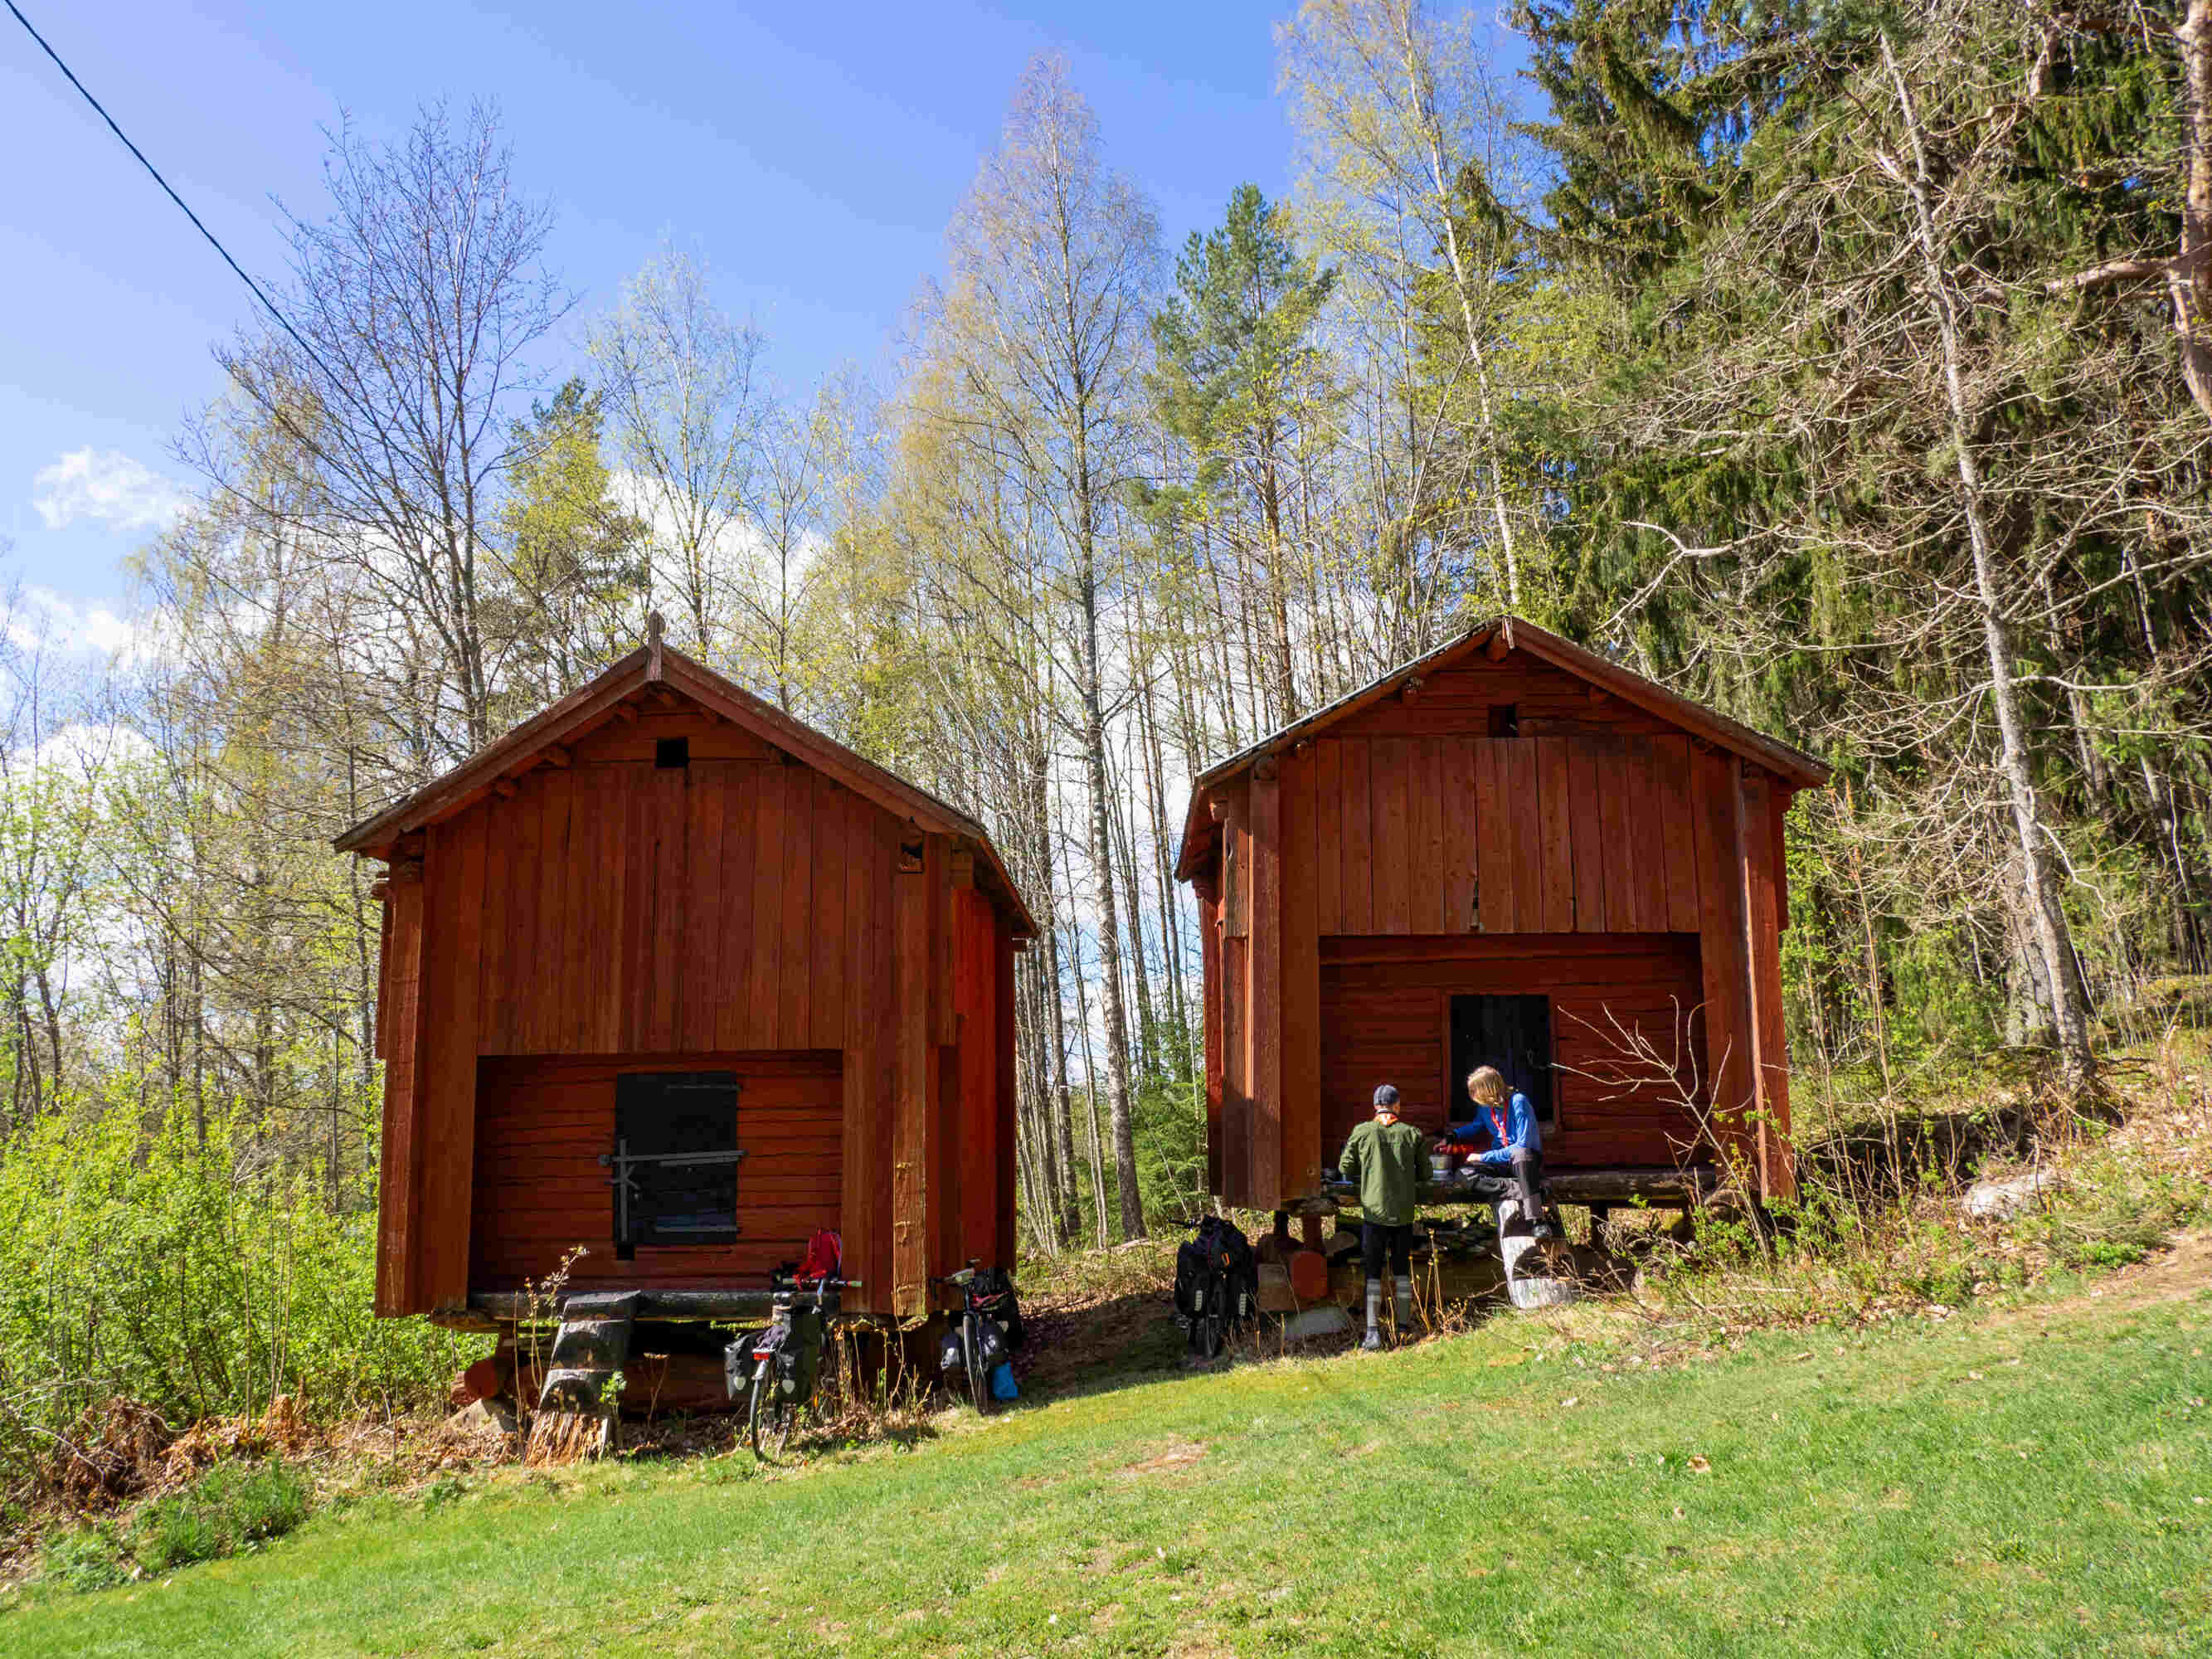
\includegraphics[width=0.94\linewidth]{assets/pyörävaellus7}
		\noindent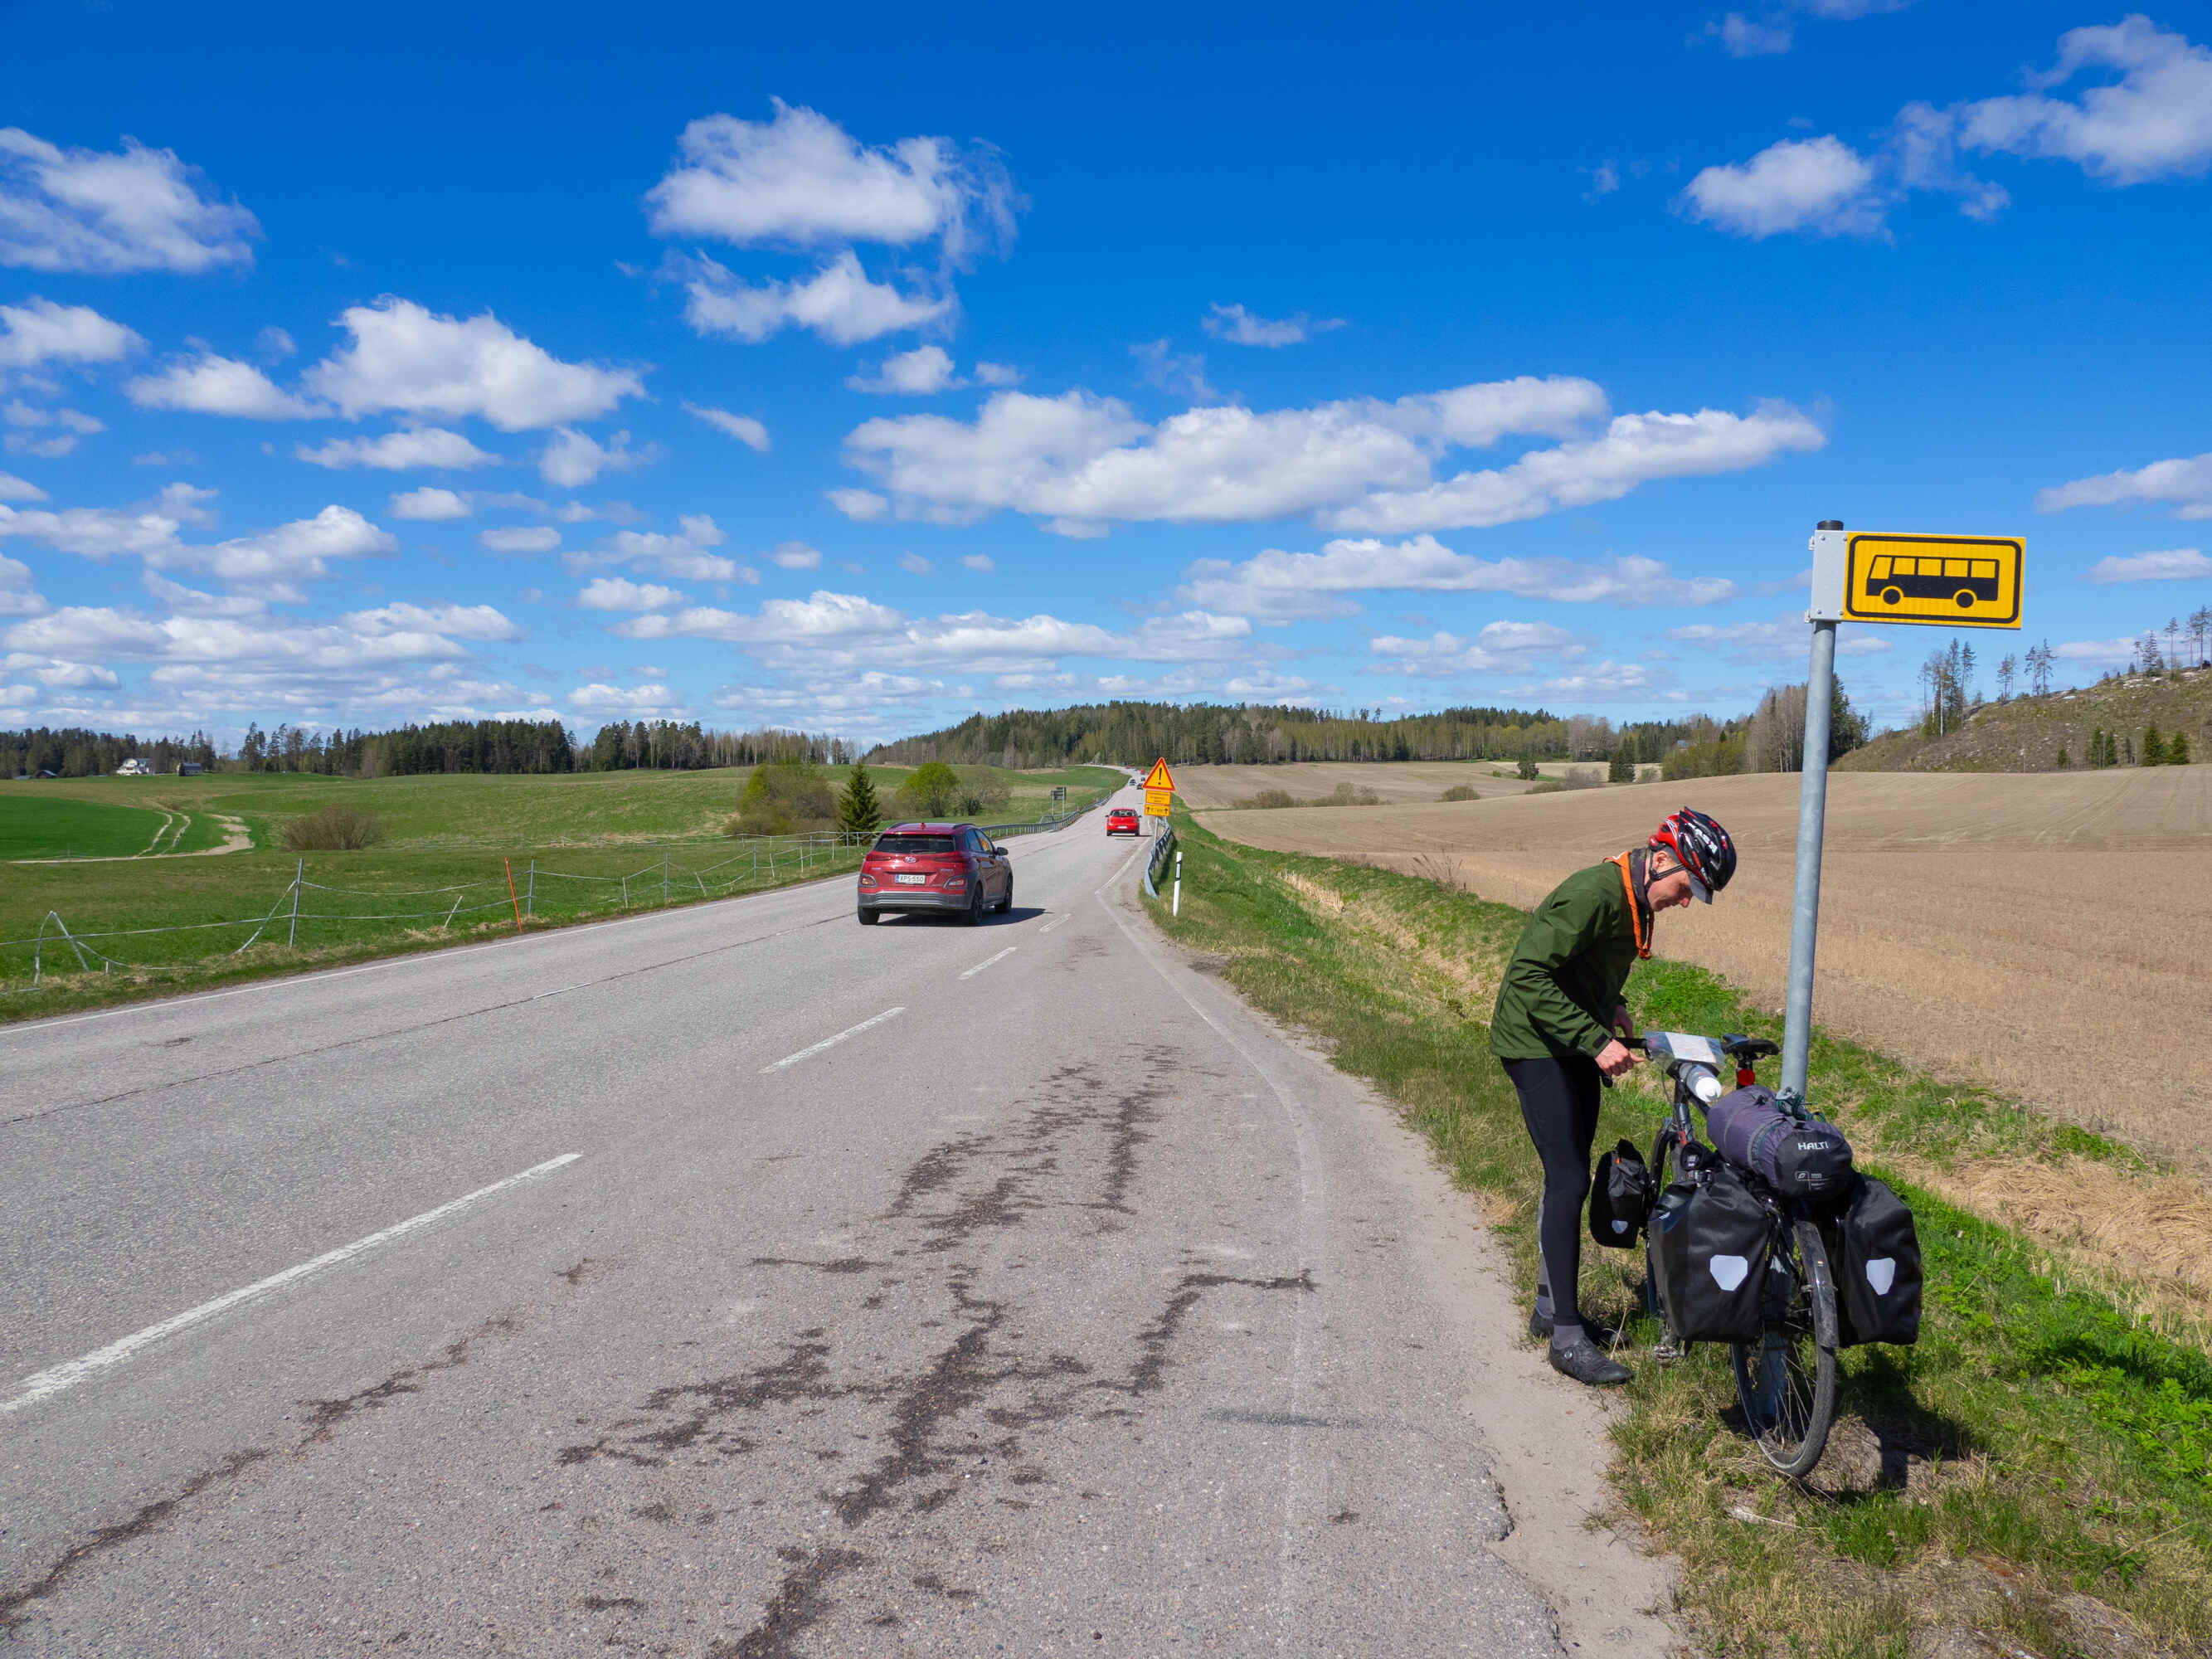
\includegraphics[width=0.94\linewidth]{assets/pyörävaellus8}
		\noindent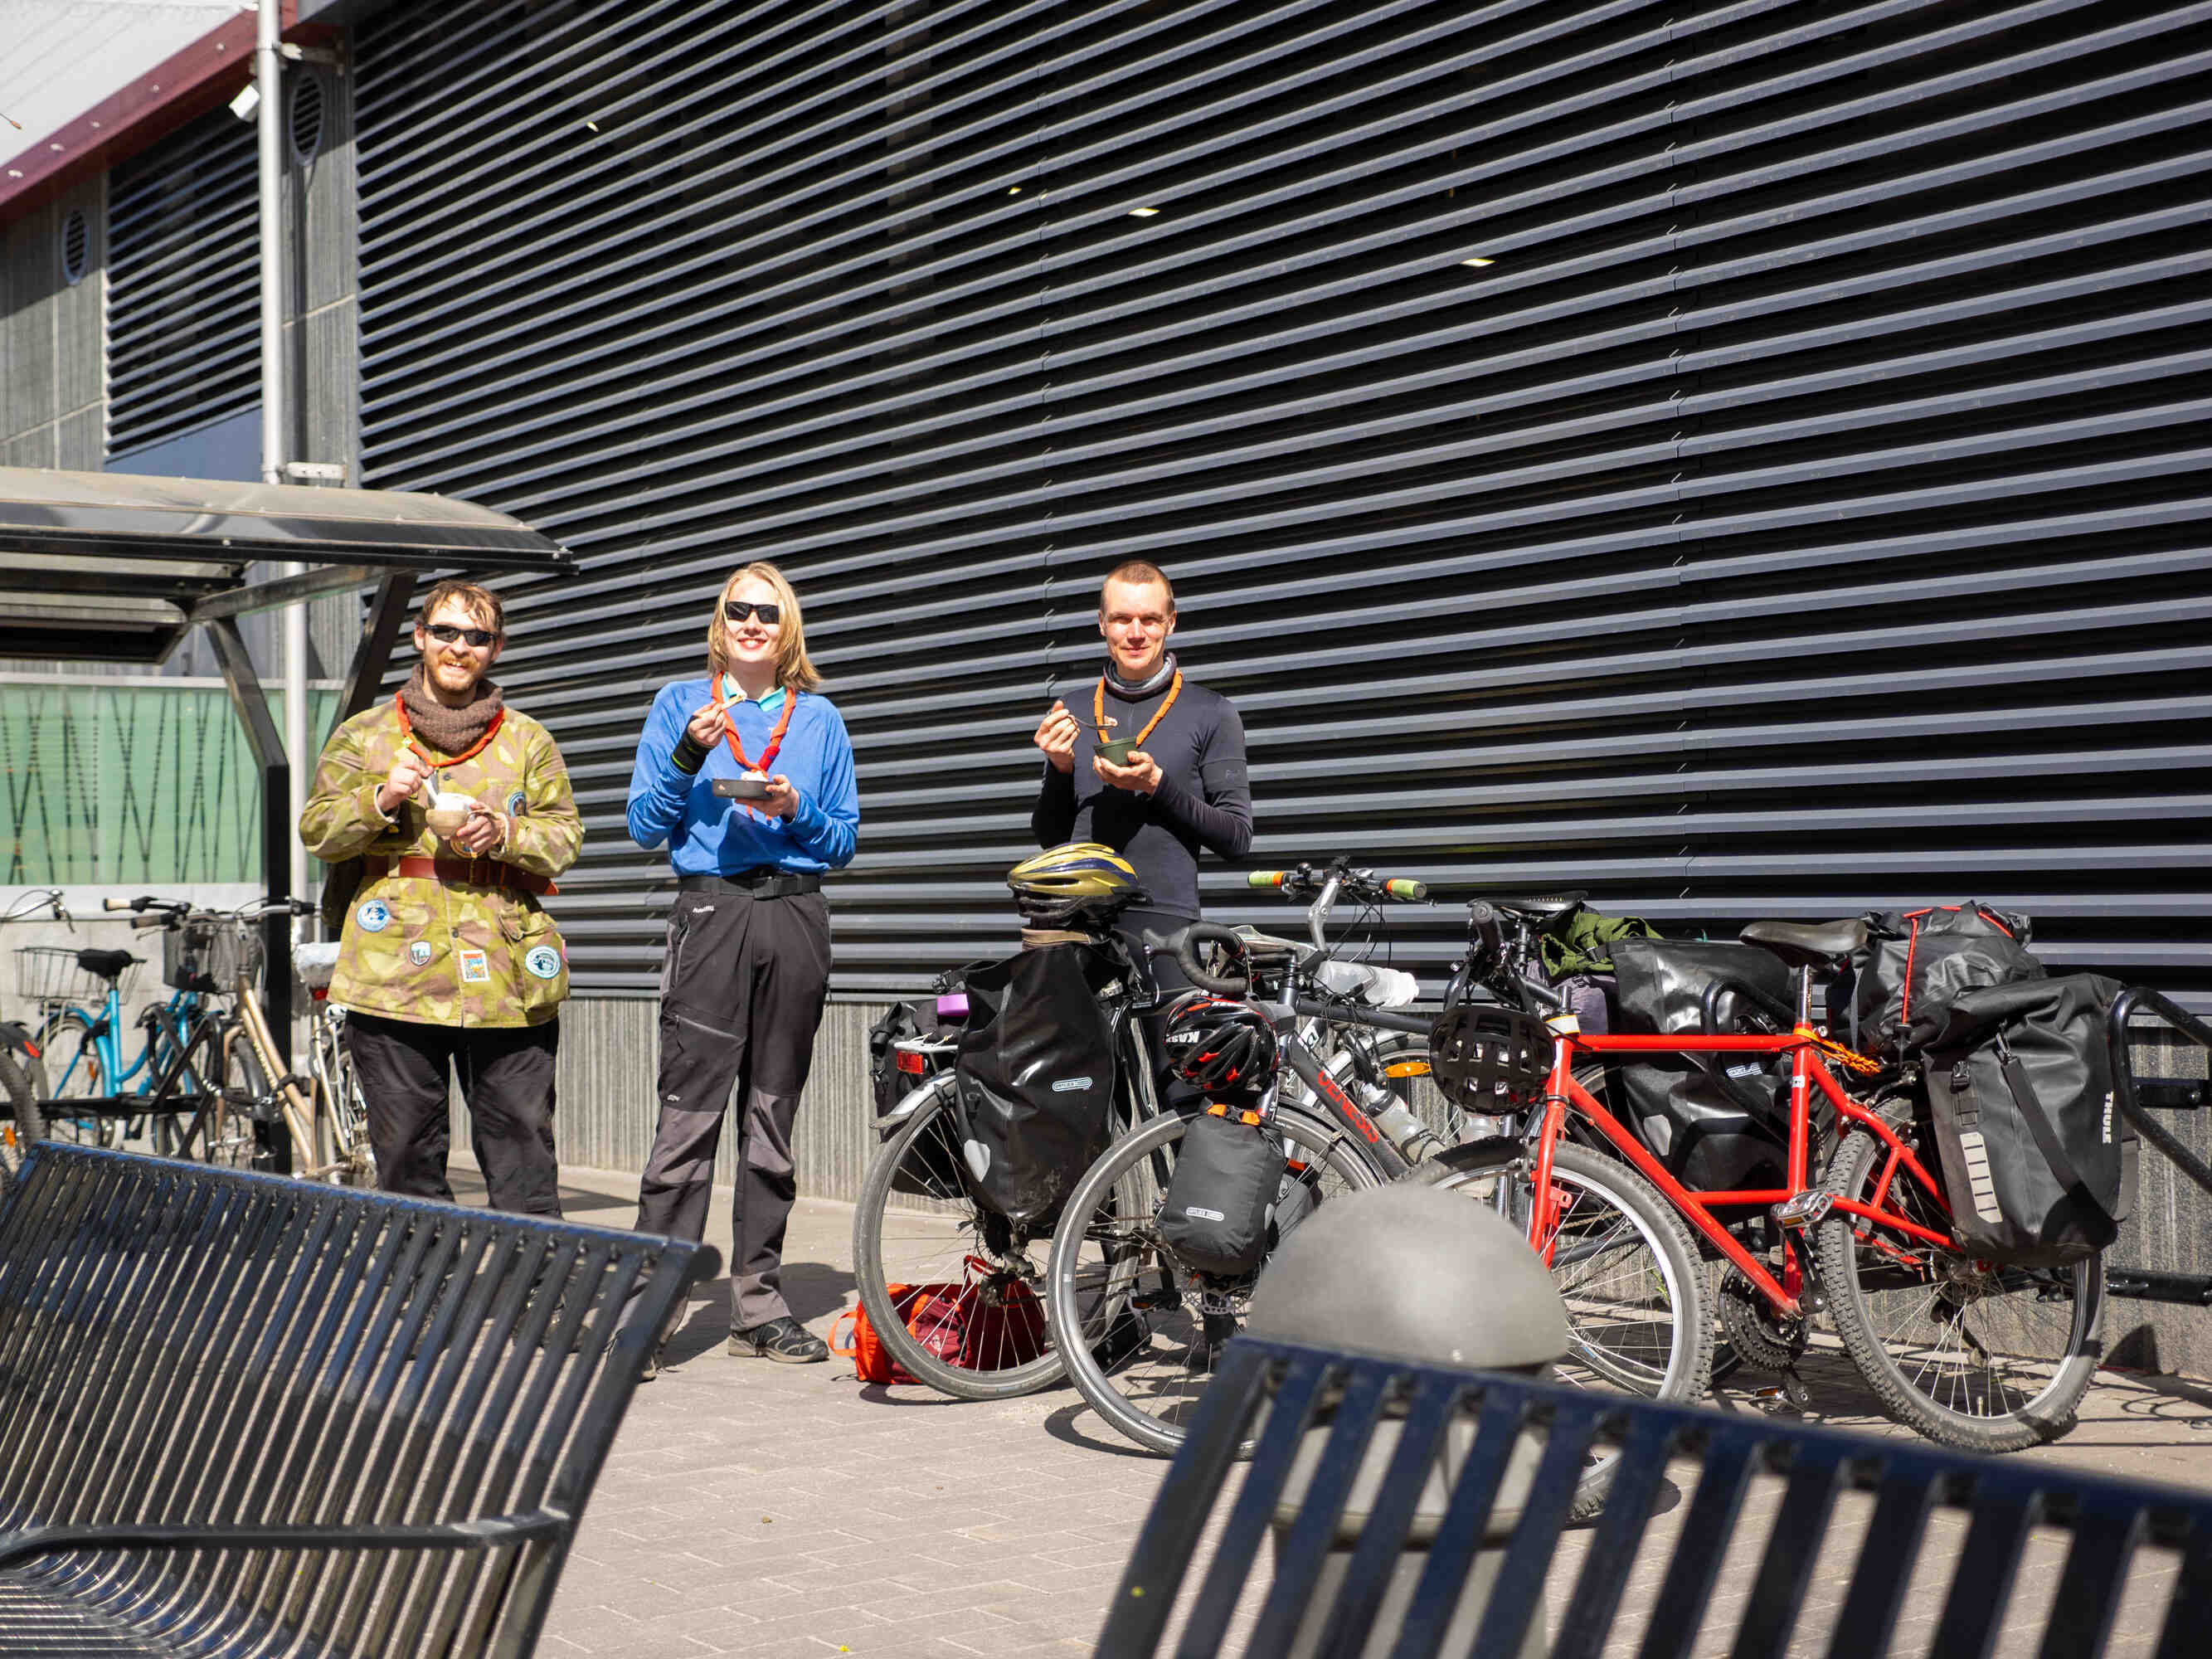
\includegraphics[width=0.94\linewidth]{assets/pyörävaellus9}
	\end{center}

	\columnbreak

	\begin{center}
		\noindent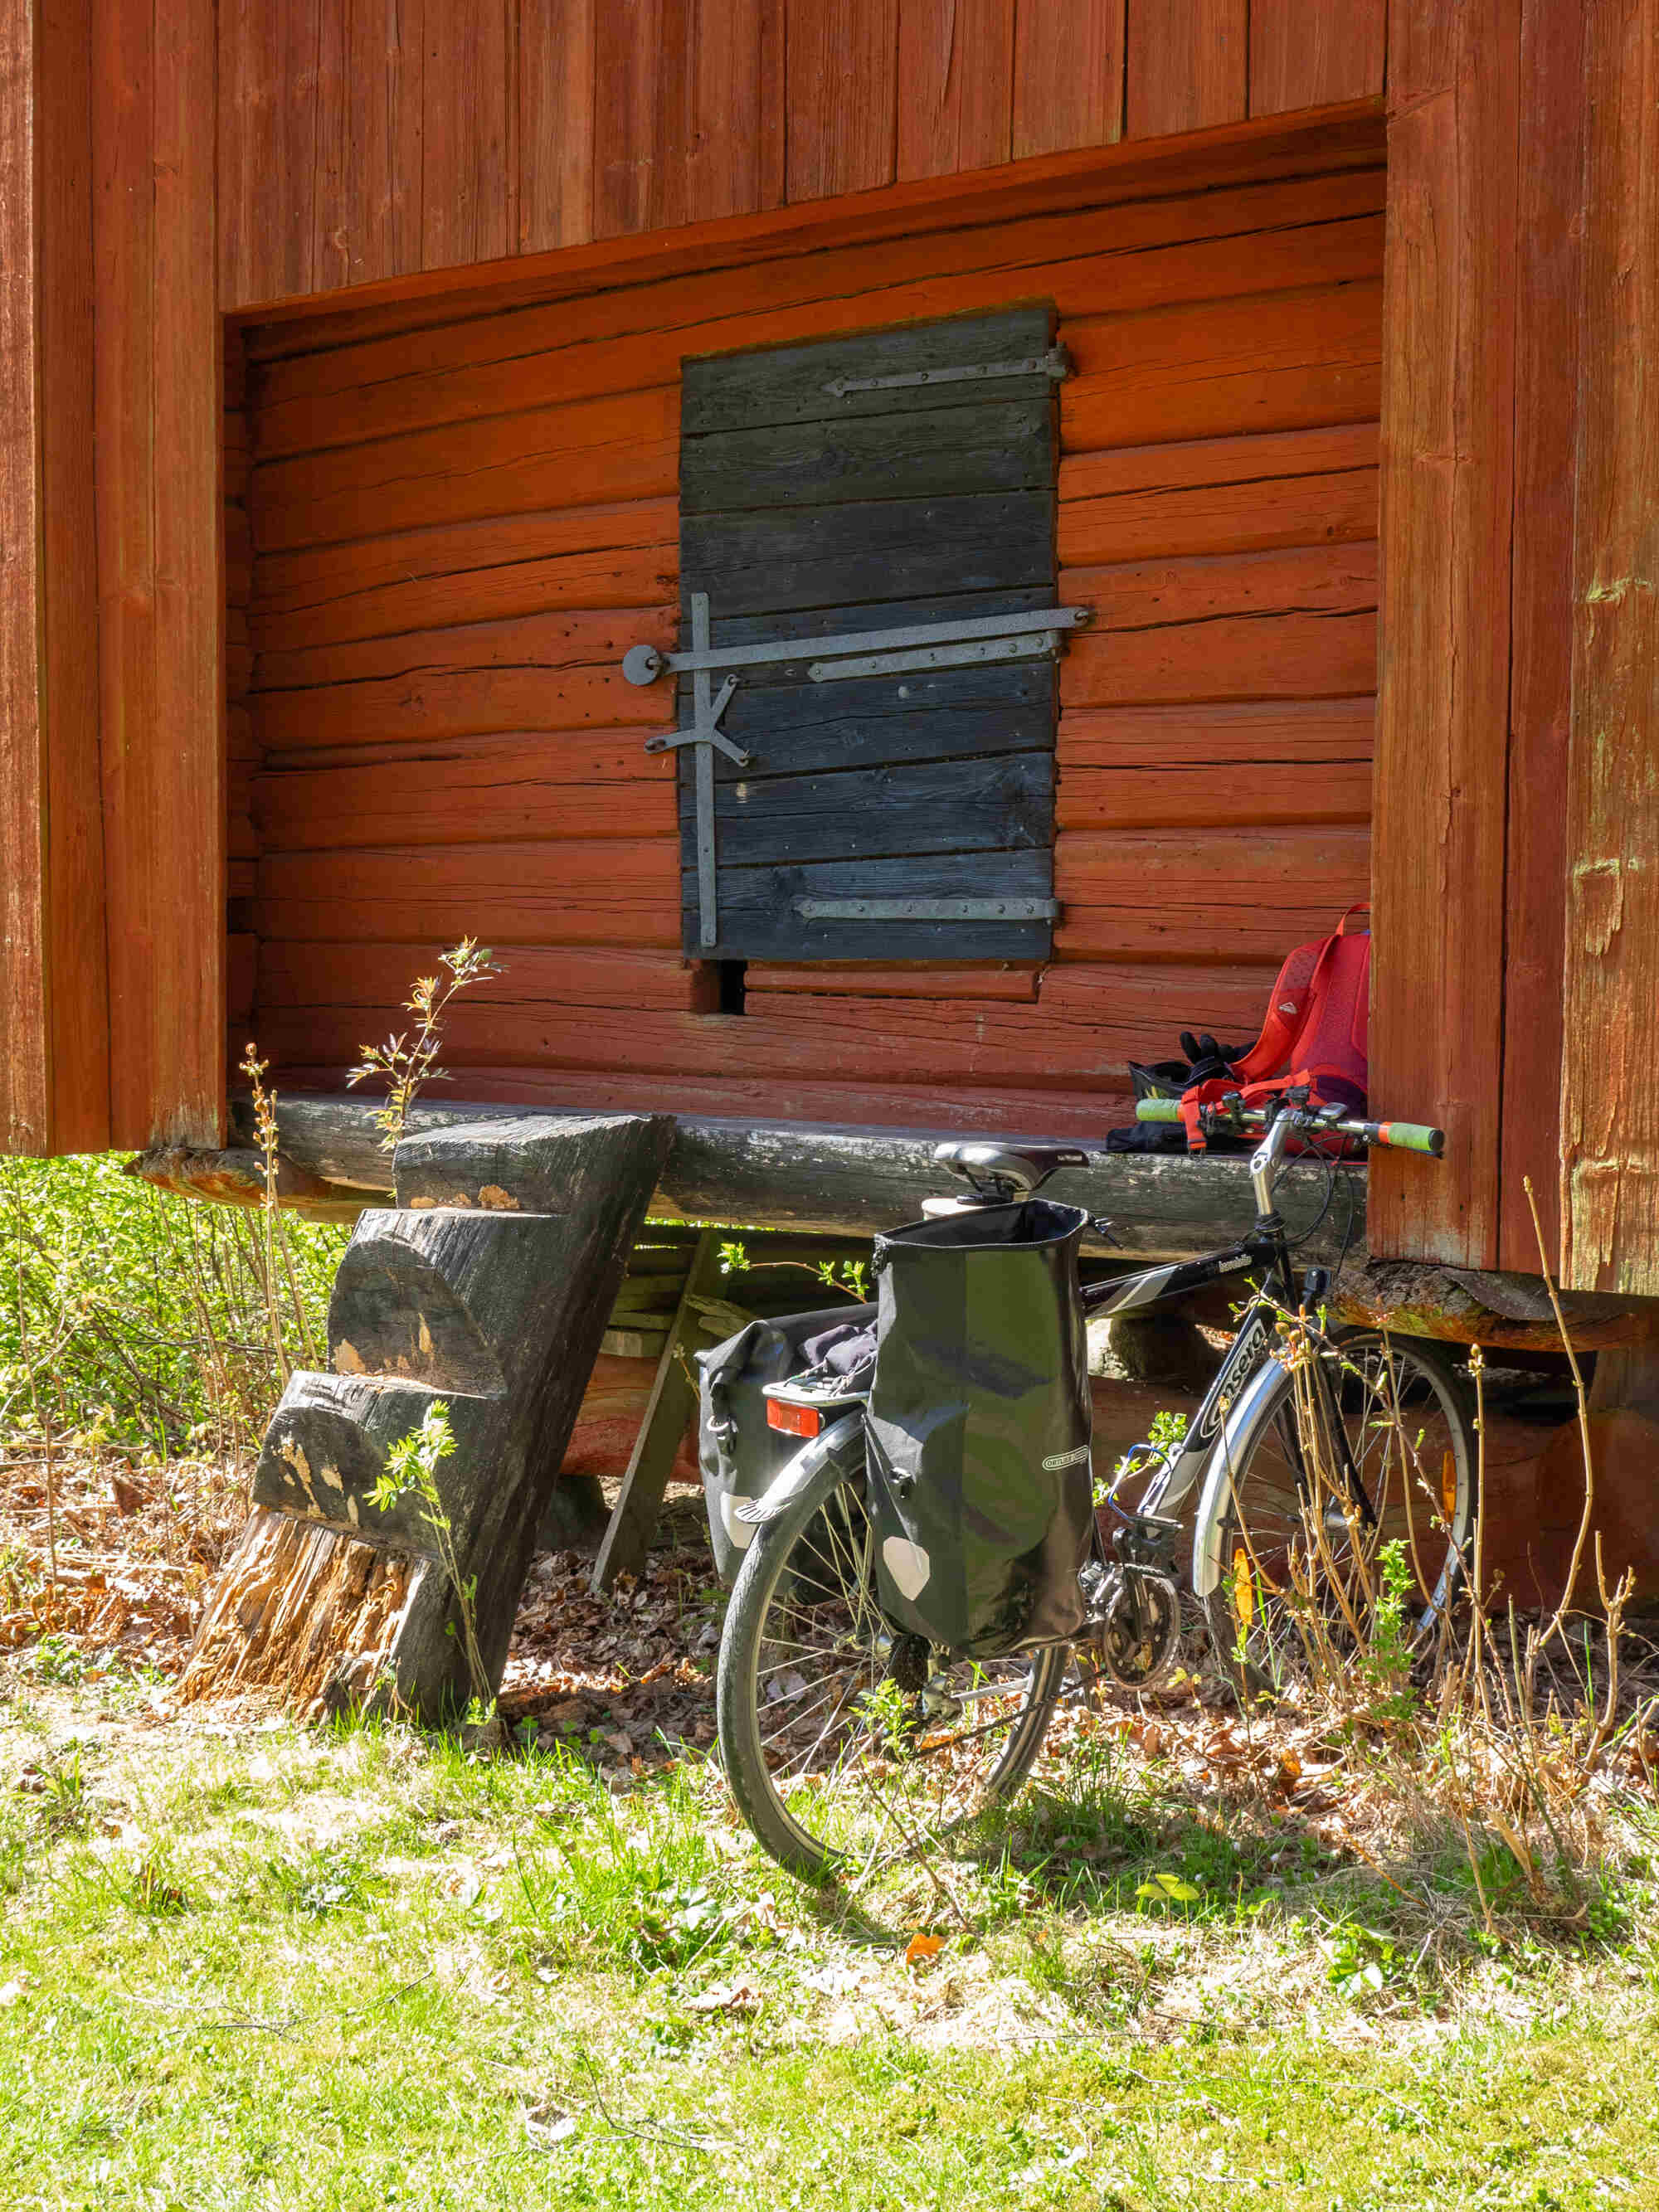
\includegraphics[width=1.05\linewidth]{assets/pyörävaellus10}
		\noindent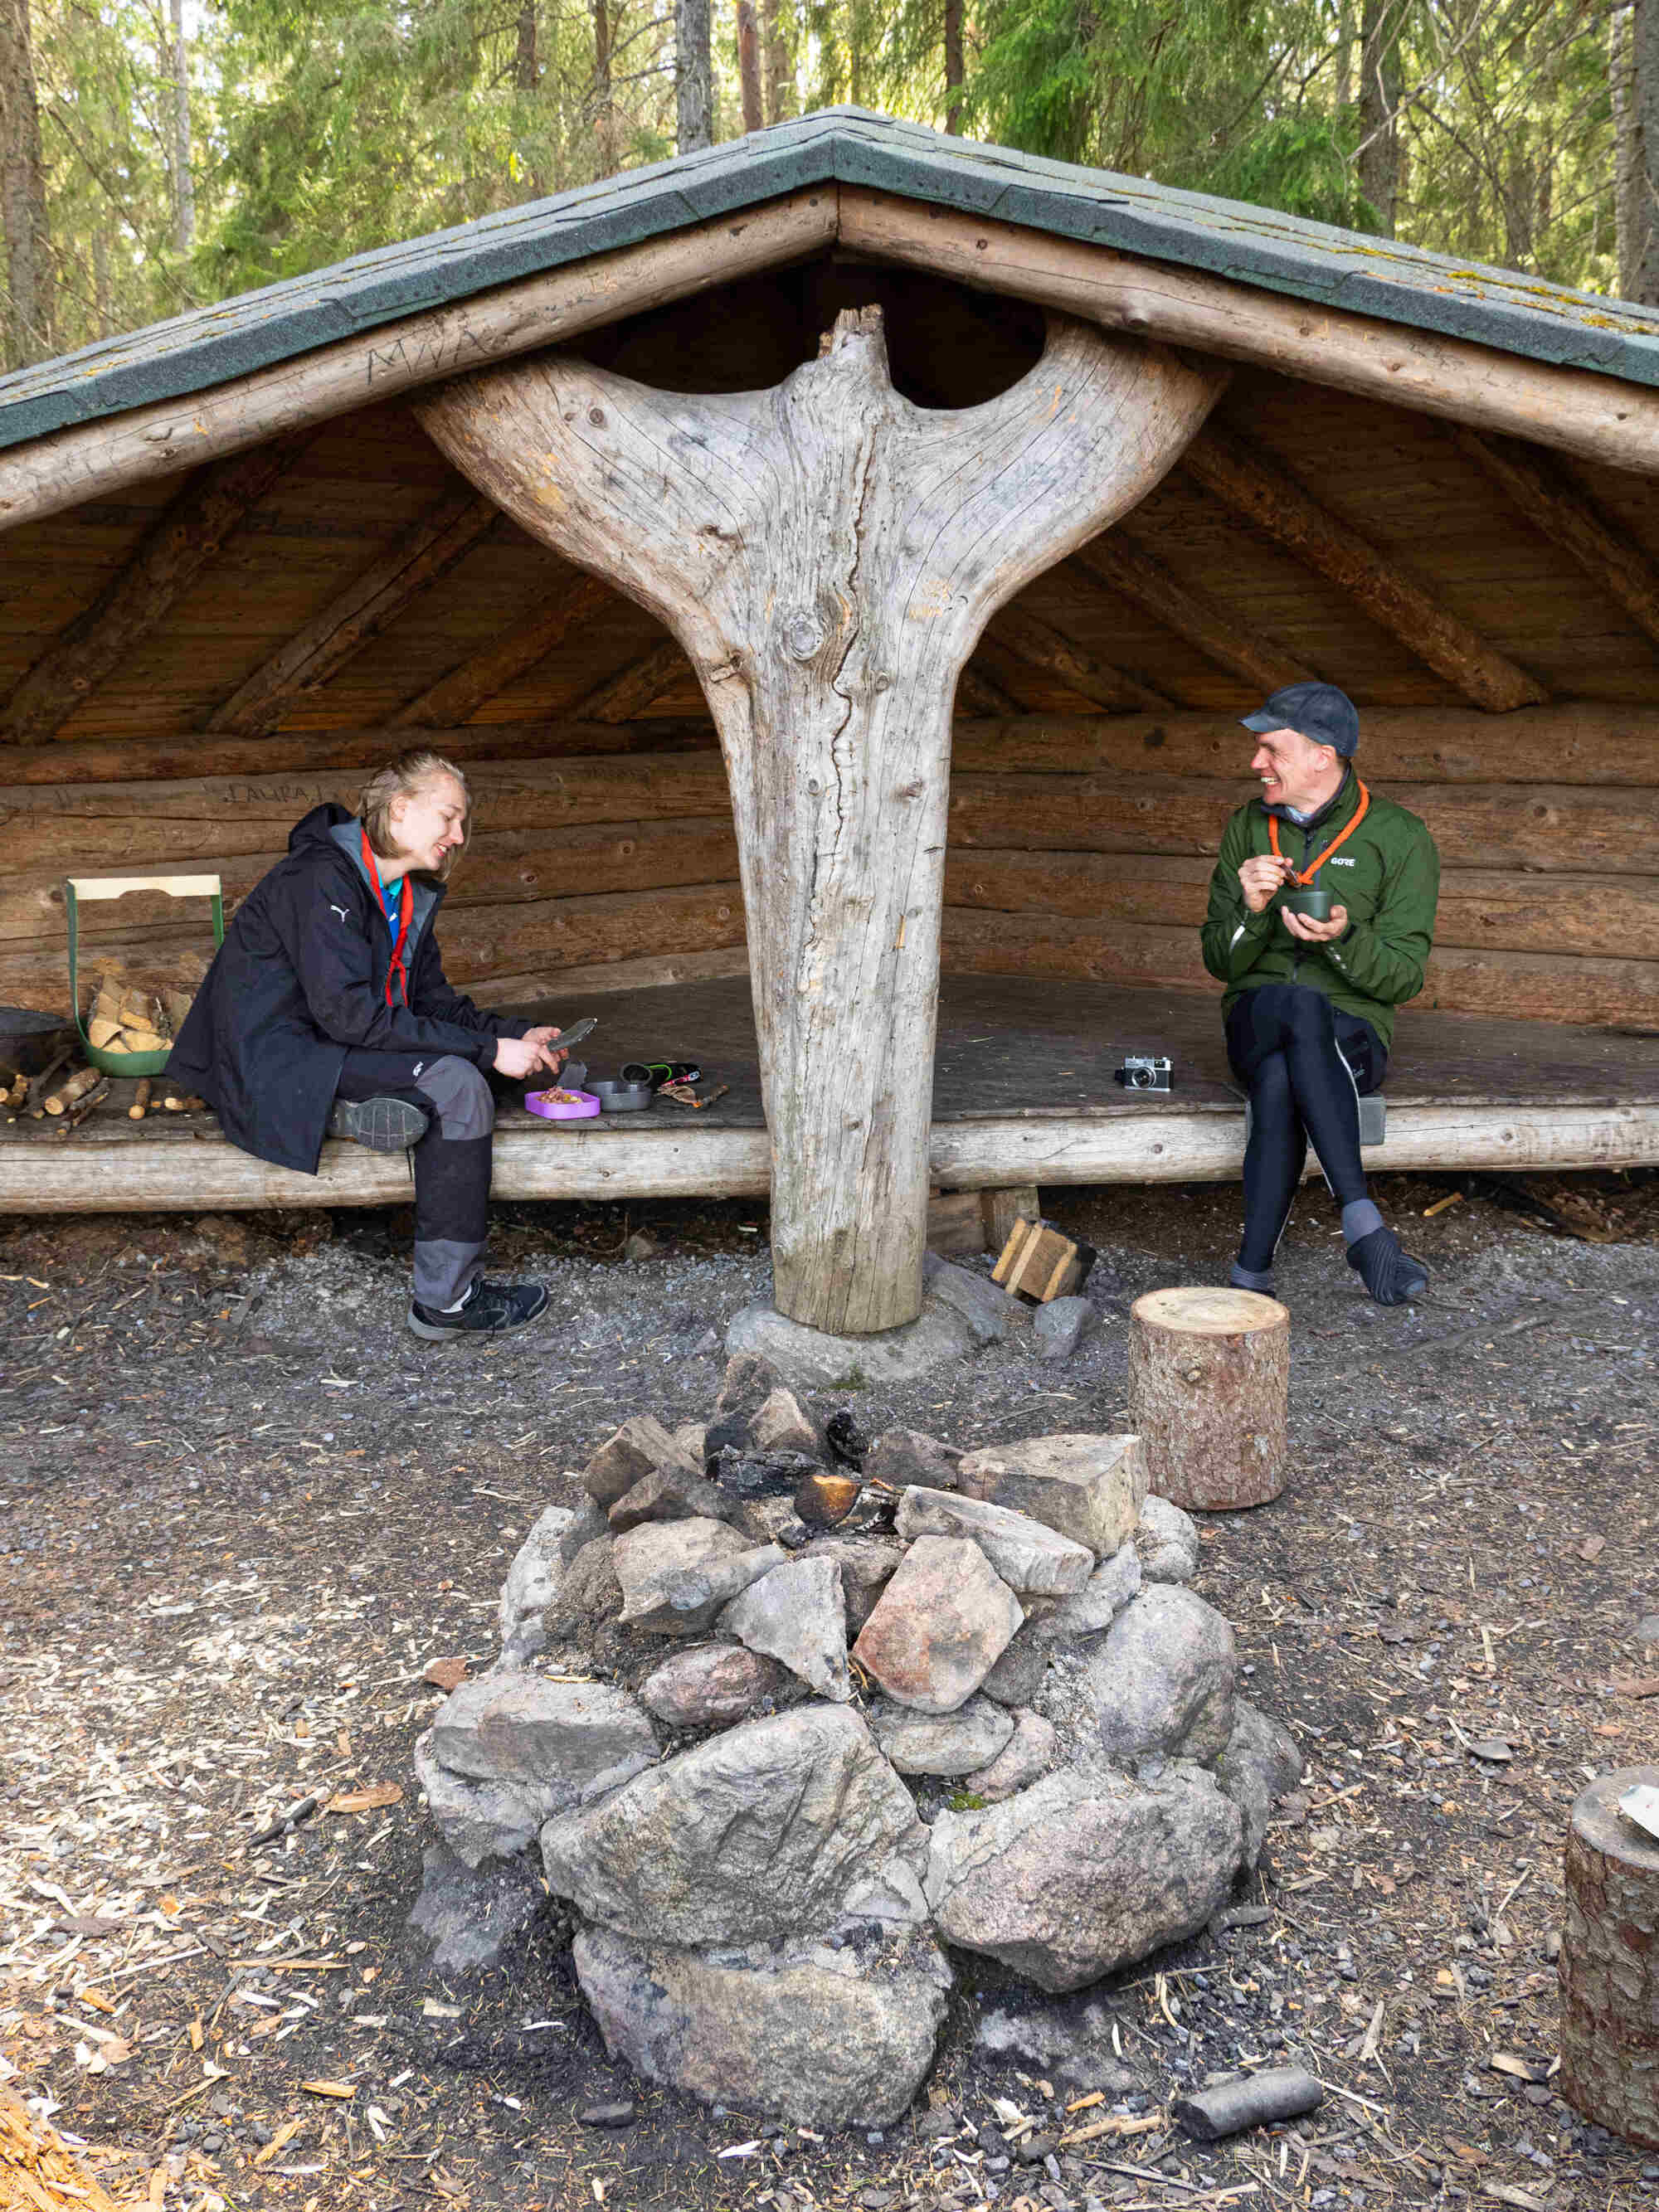
\includegraphics[width=1.05\linewidth]{assets/pyörävaellus13}
	\end{center}
	\columnbreak
	\begin{center}
		\noindent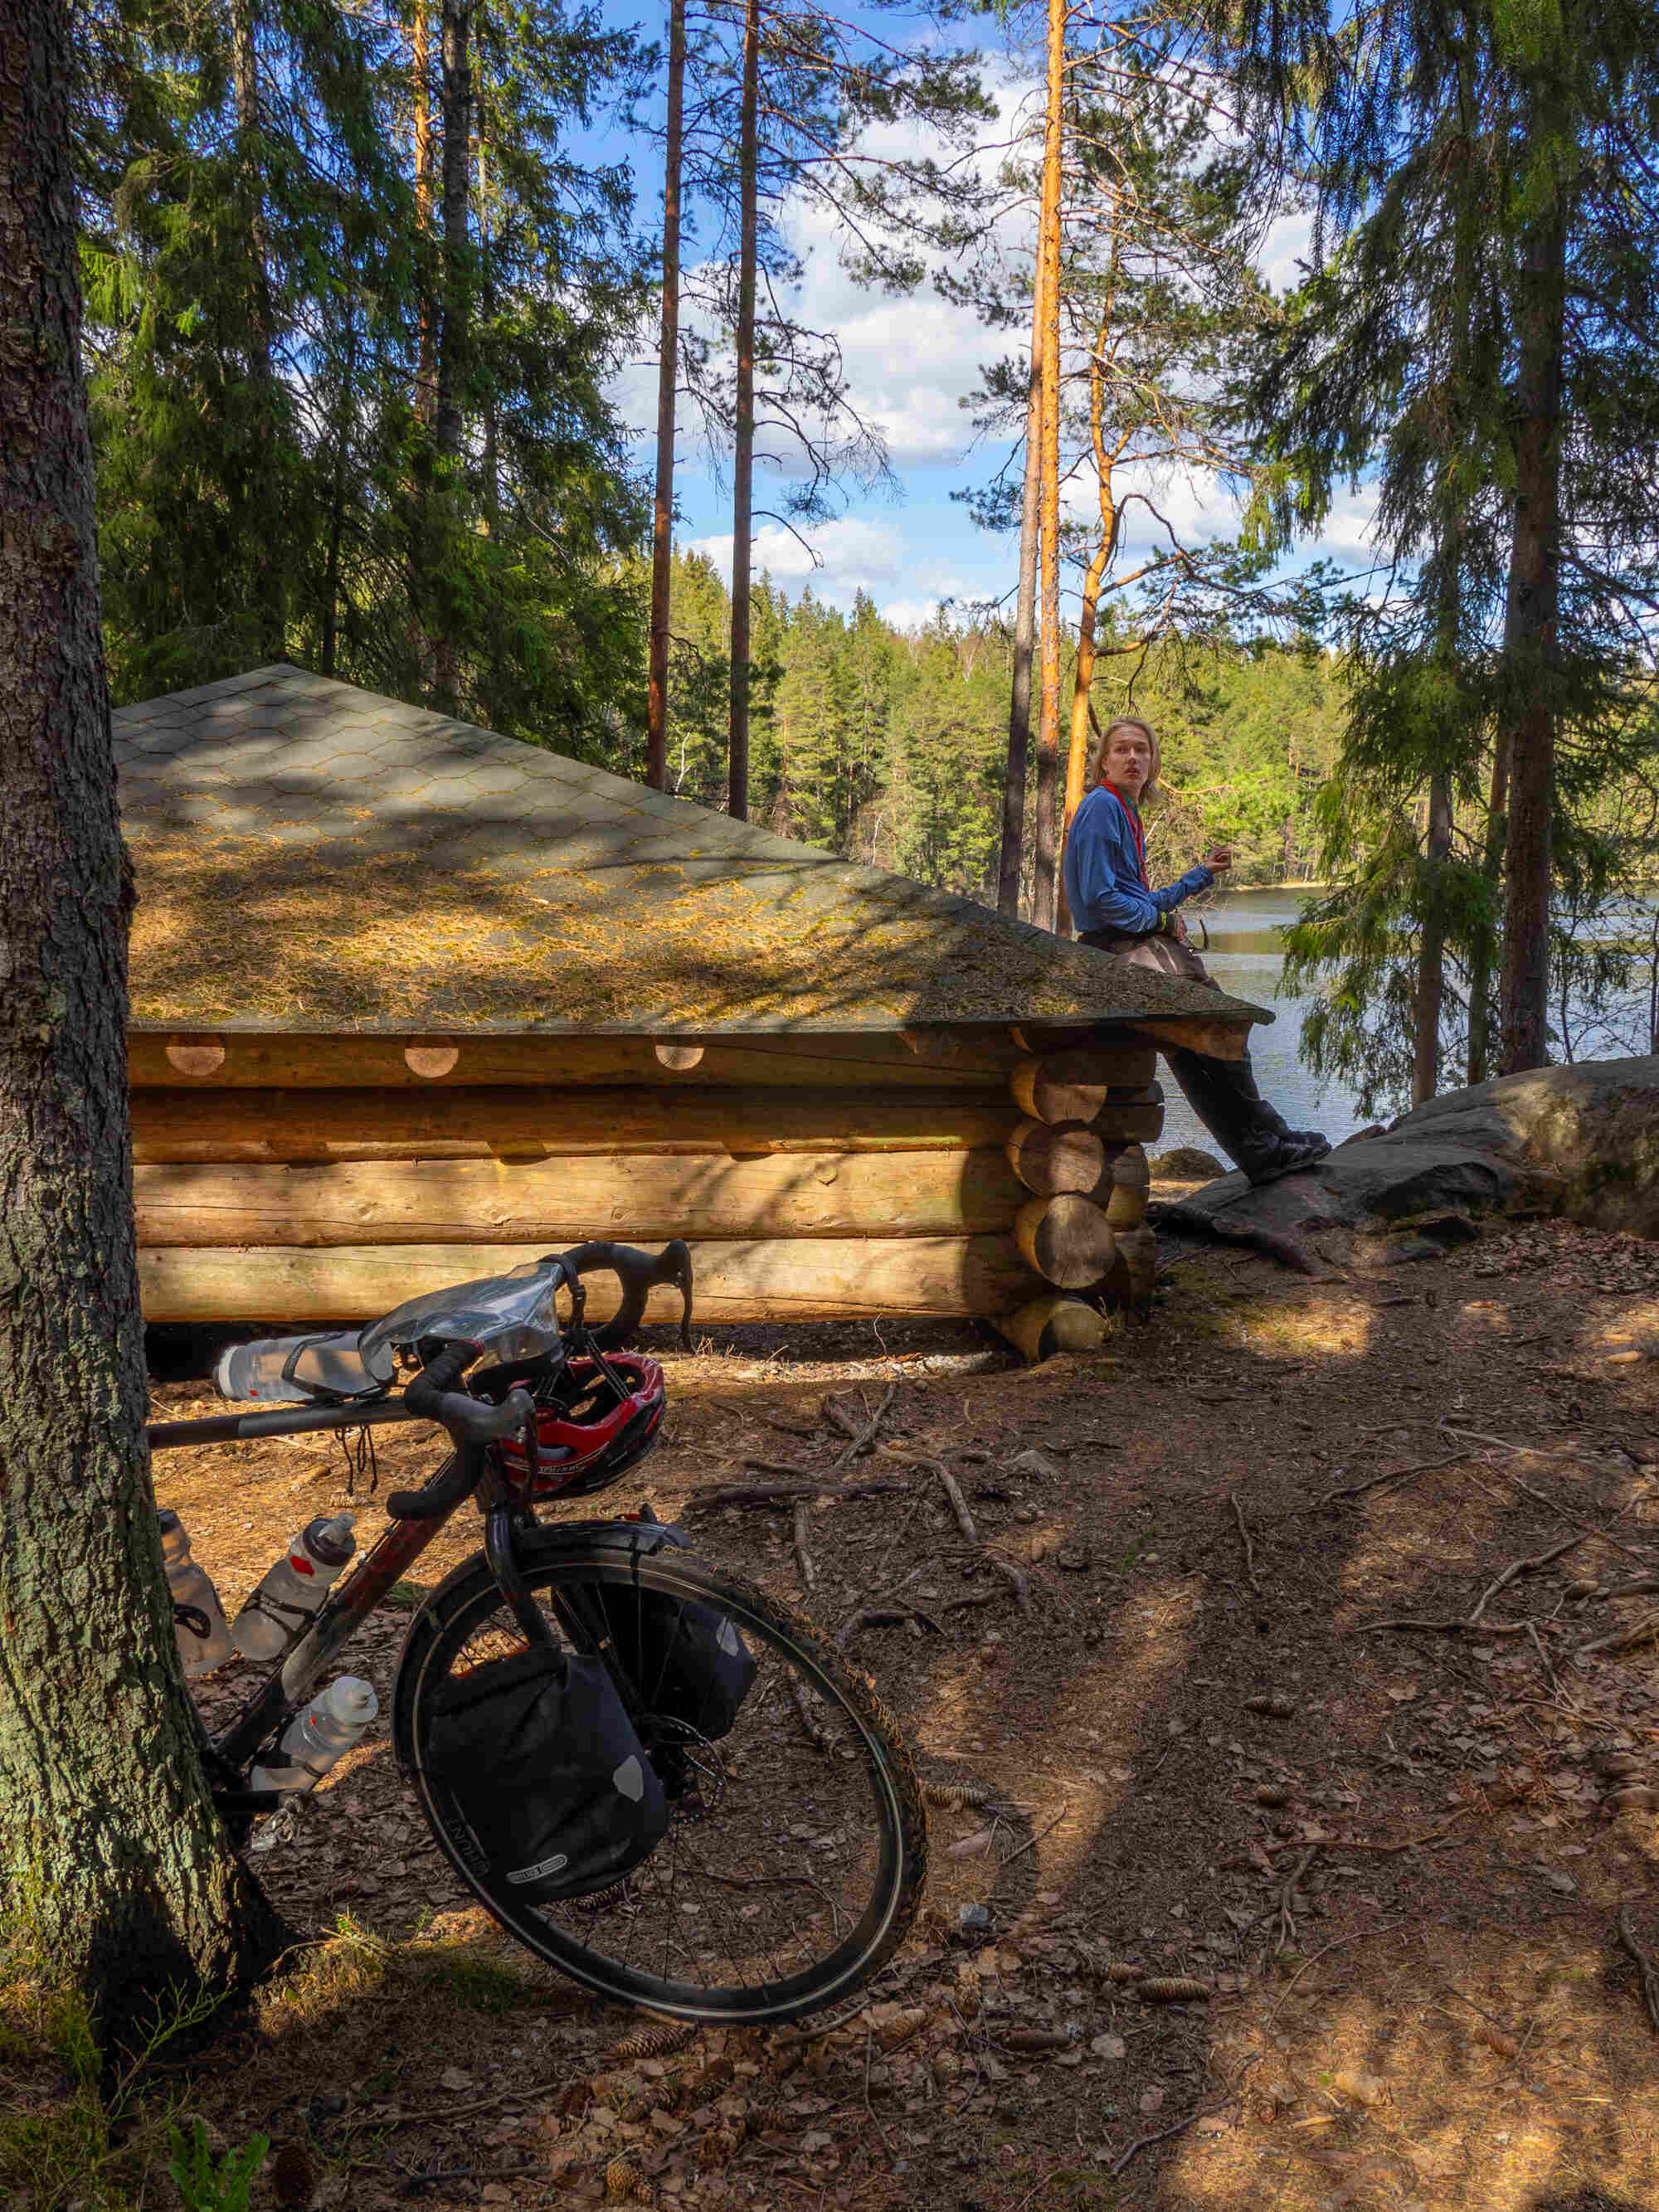
\includegraphics[width=1.05\linewidth]{assets/pyörävaellus11}
		\noindent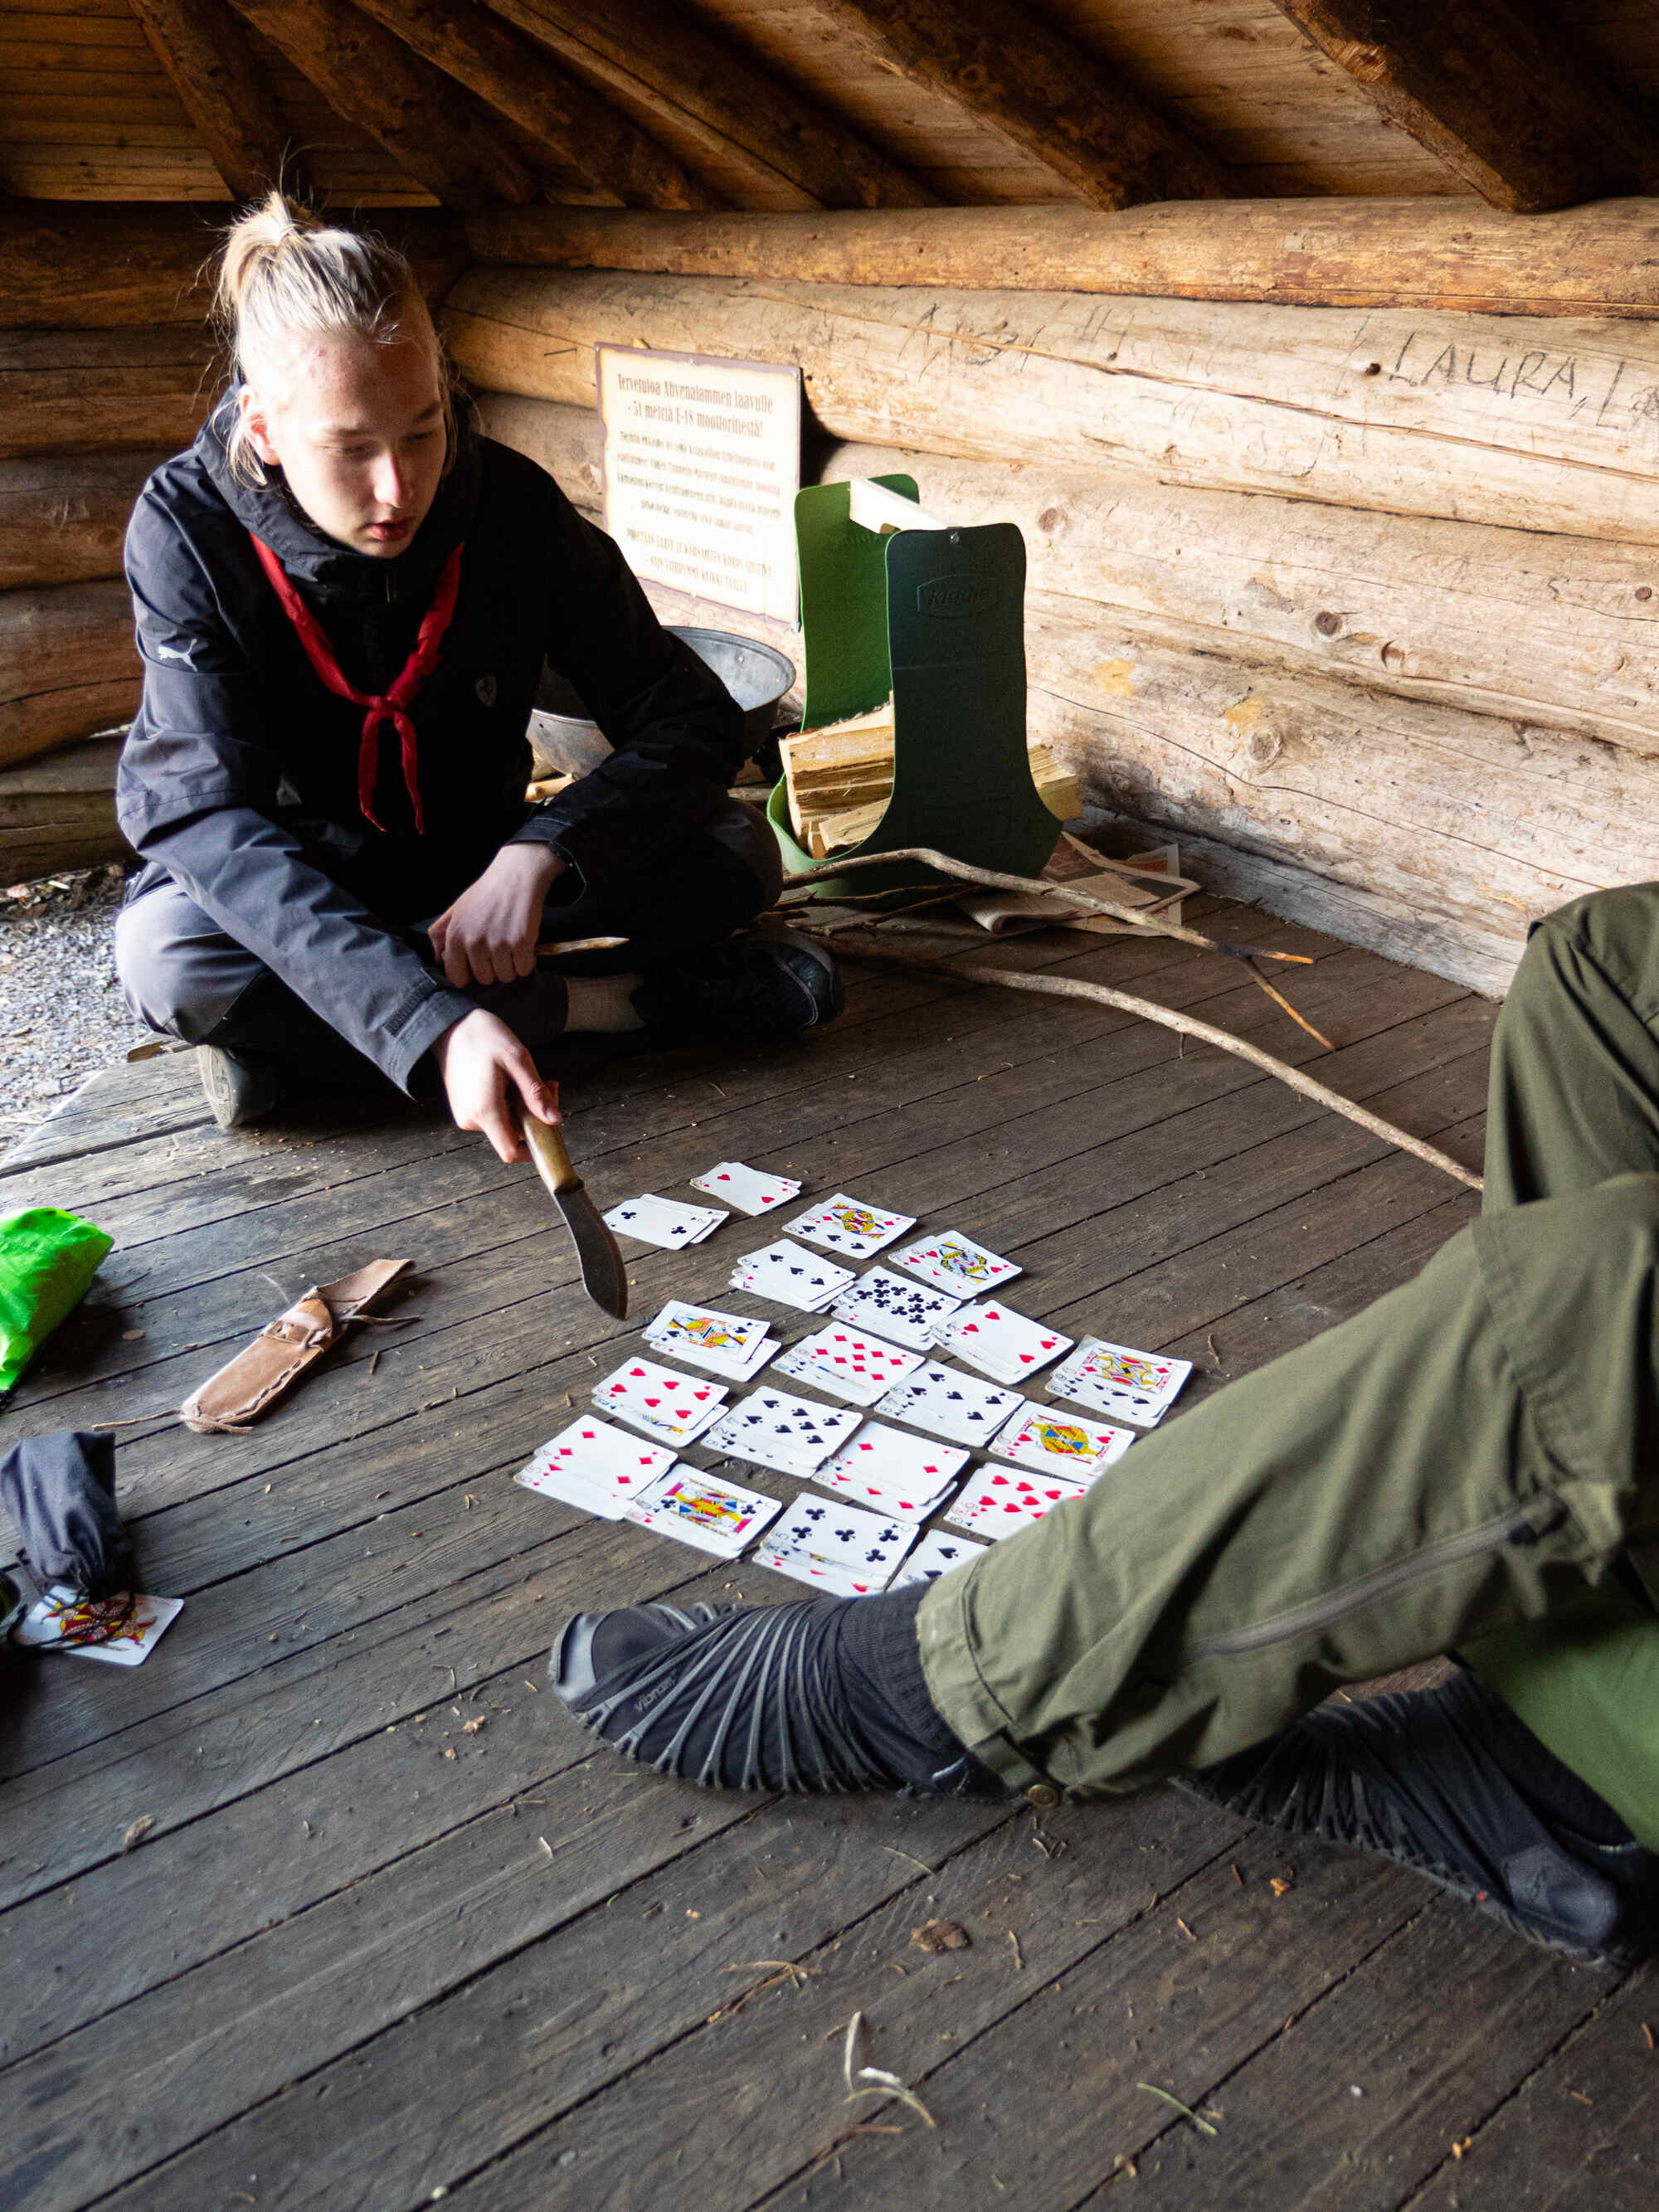
\includegraphics[width=1.05\linewidth]{assets/pyörävaellus15}
	\end{center}

	\columnbreak

	\medskip
	\noindent\null\hfill Tanguy Gérôme

\end{multicols}

\clearpage
\subsection{Kevätretki \& kevätjuhla 24.-26.5.}

\clearpage\section{Kuvakilpailu}

Tassun toimittajat toivovat julkaisevansa toisen painoksen vuoden lopussa, ja
järjestävät näiden painosten välissä kuvakilpailun!

\clearpage\section{Tulossa pian}
\subsection{Uikun uinti -vaellus 26.–30.6.}
\subsection{Kimara 26.7.-3.8.}



\clearpage

\thispagestyle{empty}\ThisCenterWallPaper{1.07}{assets/no_auto_compression/takakansikuva.jpg}~

\vfill


{
	\noindent
	\begin{center}
		\contour{white}{\Large\bfseries \color{black}1/2024 Kurkisuon Rusakot ry}
	\end{center}
	% \psset{cornersize=absolute,linearc=2.5\baselineskip}
	% \begin{center}
	% 	\psframebox[framesep=3mm,fillcolor=white,fillstyle=solid,linestyle=none]{
	% 		\color{kuru}\Large\bfseries Kurkisuon Rusakot ry\par
	% 	}
	% \end{center}
}
\end{document}
